\documentclass[a4paper]{book}

\usepackage{amsmath, amsthm, amsfonts, amssymb, mathtools, yhmath, mathrsfs}
\usepackage{tikz}
\usepackage{enumerate}
\usepackage{tcolorbox}
\usepackage[a4paper,hmargin={1cm,1cm},vmargin={2.5cm,2.5cm}]{geometry}
\usepackage{hyperref}
\usepackage{fontenc}
\usepackage{CJKutf8}

\hypersetup{unicode,backref,colorlinks=true}
%%%%%%%%%%%%%%%%%%%%%%%%%%%%%%%%%%%%%%%%%%%%%%%%%%%%%%%%%%%%%%%%%%%%%%%%%%%%%%%%%%%
%%%%%%%%%%%%%%%%%%%%%%%%%%%%%%%%%%%%%%%%%%%%%%%%%%%%%%%%%%%%%%%%%%%%%%%%%%%%%%%%%%%
%%%%%%%%%%%%%%%%%%%%%%%%%%%%%%%%%%%%%%%%%%%%%%%%%%%%%%%%%%%%%%%%%%%%%%%%%%%%%%%%%%%

% from tcolorbox.pdf
\tcbuselibrary{theorems, breakable, skins, raster, listings, minted, xparse, listingsutf8, documentation}
\newtcbtheorem[number within=section]{question}{问题}%
  {colback=green!5,colframe=green!35!black,fonttitle=\bfseries}{q}
\newtcbtheorem[number within=section]{definition}{定义}%
  {colback=blue!5,colframe=gray!50!black,fonttitle=\bfseries}{def}
\newtcbtheorem[number within=section]{lemma}{引理}%
  {colback=purple!5,colframe=purple!75!black,fonttitle=\bfseries}{lm}
\newtcbtheorem[number within=section]{theorem}{定理}%
  {colback=purple!5,colframe=purple!75!black,fonttitle=\bfseries}{th}
\newtcbtheorem[number within=section]{corrolary}{推论}%
  {colback=yellow!5,colframe=yellow!75!black,fonttitle=\bfseries}{co}
\newtcbtheorem[number within=section]{undone}{未知}%
  {colback=red!5,colframe=red!75!black,fonttitle=\bfseries}{un}
\newtcbtheorem[number within=section]{comments}{评论}%
  {colback=gray!5,colframe=gray!75!black,fonttitle=\bfseries}{cm}
\newtcbtheorem[number within=section]{answer}{解答}%
  {colback=gray!5,colframe=gray!75!black,fonttitle=\bfseries}{ans}
% from amsthdoc.pdf
\makeatletter
\renewenvironment{proof}[1][\proofname]{\par
    \pushQED{\qed}%
    \normalfont \topsep6\p@\@plus6\p@\relax
    \trivlist
    \item\relax
    {\itshape
    #1\@addpunct{.}}\hspace\labelsep\ignorespaces
  }{%
    \popQED\endtrivlist\@endpefalse
  }
\makeatother

%%%%%%%%%%%%%%%%%%%%%%%%%%%%%%%%%%%%%%%%%%%%%%%%%%%%%%%%%%%%%%%%%%%%%%%%%%%%%%%%%%%
%%%%%%%%%%%%%%%%%%%%%%%%%%%%%%%%%%%%%%%%%%%%%%%%%%%%%%%%%%%%%%%%%%%%%%%%%%%%%%%%%%%
%%%%%%%%%%%%%%%%%%%%%%%%%%%%%%%%%%%%%%%%%%%%%%%%%%%%%%%%%%%%%%%%%%%%%%%%%%%%%%%%%%%

\def\degree{^\circ}
\def\bq{\begin{question}}
\def\eq{\end{question}}
\def\bqq{\begin{question*}}
\def\eqq{\end{question*}}
\def\bt{\begin{theorem}}
\def\et{\end{theorem}}
\def\bl{\begin{lemma}}
\def\el{\end{lemma}}
\def\bd{\begin{definition}}
\def\ed{\end{definition}}
\def\bc{\begin{corrolary}}
\def\ec{\end{corrolary}}
\def\bm{\begin{comments*}{}{}}
\def\em{\end{comments*}}
\def\bu{\begin{undone}}
\def\eu{\end{undone}}
\def\ba{\begin{proof}[解]}
\def\ea{\end{proof}}
\def\bs{\begin{answer*}{}{}}
\def\es{\end{answer*}}
\def\ue{\mathrm{e}}
\def\ud{\,\mathrm{d}}
\def\ui{\mathrm{i}}
\def\Re{\mathrm{Re}}
\def\Im{\mathrm{Im}}
\def\Res{\mathrm{Res}}
\def\diag{\,\mathrm{diag}\,}
\def\be{\begin{equation}}
\def\ee{\end{equation}}
\def\bee{\begin{equation*}}
\def\eee{\end{equation*}}
\def\sumcyc{\sum\limits_{cyc}}
\def\prodcyc{\prod\limits_{cyc}}
\def\i{\infty}
\def\a{\alpha}
\def\b{\beta}
\def\g{\gamma}
\def\d{\delta}
\def\l{\lambda}
\def\m{\mu}
\def\t{\theta}

%%%%%%%%%%%%%%%%%%%%%%%%%%%%%%%%%%%%%%%%%%%%%%%%%%%%%%%%%%%%%%%%%%%%%%%%%%%%%%%%%%%
%%%%%%%%%%%%%%%%%%%%%%%%%%%%%%%%%%%%%%%%%%%%%%%%%%%%%%%%%%%%%%%%%%%%%%%%%%%%%%%%%%%
%%%%%%%%%%%%%%%%%%%%%%%%%%%%%%%%%%%%%%%%%%%%%%%%%%%%%%%%%%%%%%%%%%%%%%%%%%%%%%%%%%%

\providecommand{\abs}[1]{\left\lvert#1\right\rvert}
\providecommand{\norm}[1]{\lVert#1\rVert}
\providecommand{\paren}[1]{\left(#1\right)}

%%%%%%%%%%%%%%%%%%%%%%%%%%%%%%%%%%%%%%%%%%%%%%%%%%%%%%%%%%%%%%%%%%%%%%%%%%%%%%%%%%%
%%%%%%%%%%%%%%%%%%%%%%%%%%%%%%%%%%%%%%%%%%%%%%%%%%%%%%%%%%%%%%%%%%%%%%%%%%%%%%%%%%%
%%%%%%%%%%%%%%%%%%%%%%%%%%%%%%%%%%%%%%%%%%%%%%%%%%%%%%%%%%%%%%%%%%%%%%%%%%%%%%%%%%%

\newcommand{\Integers}{\mathbb{Z}}
\newcommand{\Naturals}{\mathbb{N}}
\newcommand{\Rationals}{\mathbb{Q}}
\newcommand{\Reals}{\mathbb{R}}
\newcommand{\pNaturals}{\mathbb{N}_{+}}
\DeclareTotalTCBox{\cmd}{ s v }
{verbatim,colupper=white,colback=black!75!white,colframe=black}
{\IfBooleanTF{#1}{\textcolor{green}{\ttfamily\bfseries \$ }}{}%
\lstinline[language=sh,keywordstyle=\color{blue!35!white}\bfseries]^#2^}
   
%%%%%%%%%%%%%%%%%%%%%%%%%%%%%%%%%%%%%%%%%%%
% all the minted language can be found in http://pygments.org/languages/
\newtcbinputlisting{\inputcode}[2][]{%
  listing engine=minted,minted language=#1,minted style=igor,%manni, igor, lovelace, xcode, vim, autumn, vs, rrt, 
  %native,perldoc,borland, tango, monokai, paraiso-dark, murphy, bw, pastie, algol_nu, paraiso-light, trac, default, algol, 
  %fruity, emacs, colorful, friendly
  minted options={fontsize=\small, linenos, autogobble, breaklines, numbersep=3mm, escapeinside=||},
  listing file={#2}, title={\hspace{-8mm} #2}, 
  colback=gray!10, colframe=gray!75!black,
  listing only,breakable,
  left=9mm, enhanced,
  overlay={\begin{tcbclipinterior}\fill[darkgray!20!white] (frame.south west)
    rectangle ([xshift=8mm]frame.north west);\end{tcbclipinterior}}}

% \newtcblisting{C}{listing engine=minted,minted style=fruity,
%   minted language=C,minted options={fontsize=\small, linenos, autogobble, breaklines, numbersep=3mm, escapeinside=||},
%   colback=black!70,colframe=gray!75!black,listing only,breakable,
%   left=9mm,enhanced,
%   overlay={\begin{tcbclipinterior}\fill[darkgray!20!white] (frame.south west)
%     rectangle ([xshift=8mm]frame.north west);\end{tcbclipinterior}}}

\newtcblisting{java}{listing engine=minted,minted style=fruity,
  minted language=java,minted options={fontsize=\small, linenos, autogobble, breaklines, numbersep=3mm, escapeinside=||},
  colback=black!70,colframe=gray!75!black,listing only,breakable,
  left=9mm,enhanced,
  overlay={\begin{tcbclipinterior}\fill[darkgray!20!white] (frame.south west)
    rectangle ([xshift=8mm]frame.north west);\end{tcbclipinterior}}}

\newtcblisting{javascript}{listing engine=minted,minted style=fruity,
  minted language=java,minted options={fontsize=\small, linenos, autogobble, breaklines, numbersep=3mm, escapeinside=||},
  colback=black!70,colframe=gray!75!black,listing only,breakable,
  left=9mm,enhanced,
  overlay={\begin{tcbclipinterior}\fill[darkgray!20!white] (frame.south west)
    rectangle ([xshift=8mm]frame.north west);\end{tcbclipinterior}}}

\newtcblisting{shell}{listing engine=minted,minted style=emacs,
  minted language=sh,minted options={fontsize=\small, autogobble, breaklines, escapeinside=||},
  colback=red!60!green!50,colframe=gray!75!black,listing only,breakable,
  left=5mm,enhanced}
    
\newtcblisting{cpp}{listing engine=minted,minted style=fruity,
  minted language=c++,minted options={fontsize=\small, linenos, autogobble, breaklines, numbersep=3mm, escapeinside=||},
  colback=black!70,colframe=gray!75!black,listing only,breakable,
  left=9mm,enhanced,
  overlay={\begin{tcbclipinterior}\fill[darkgray!20!white] (frame.south west)
    rectangle ([xshift=8mm]frame.north west);\end{tcbclipinterior}}}
    
\newtcblisting{python}{listing engine=minted,minted style=fruity,
  minted language=python,minted options={fontsize=\small, linenos, autogobble, breaklines, numbersep=3mm, escapeinside=||},
  colback=black!70,colframe=gray!75!black,listing only,breakable,
  left=9mm,enhanced,
  overlay={\begin{tcbclipinterior}\fill[darkgray!20!white] (frame.south west)
    rectangle ([xshift=8mm]frame.north west);\end{tcbclipinterior}}}


\begin{document}
\begin{CJK}{UTF8}{gbsn}
\tableofcontents
%%%%%%%%%%%%%%%%%%%%%%%%%%%%%%%%%%%%%%%%%%%%%%%%%%%%%%%%%%%%%%%%%%%%%%%%%%%%%%
%%%%%%%%%%%%%%%%%%%%%%%%%%%%%%%%%%%%%%%%%%%%%%%%%%%%%%%%%%%%%%%%%%%%%%%%%%%%%%
%%%%%%%%%%%%%%%%%%%%%%%%%%%%%%%%%%%%%%%%%%%%%%%%%%%%%%%%%%%%%%%%%%%%%%%%%%%%%%

% \chapter{高中笔记8}
\section{读书笔记}
康托尔: 德, 数学家, 集合论的创造人, 他证明了一条直线上的点和一个平面上的点一一对应, 也能和空间中的点一一对应.
因此1cm长的线段内的点与太平洋面上的点以及整个地球内部的点都``一样多". 他对这类``无穷集合"问题发表了一系列文章,
通过严格证明得出了许多惊人的结论.

罗素悖论: 又称理发师悖论: 某村只有一人会理发, 且该村的人都需要理发, 理发师约定, 给且只给村中自己不给自己理发的人理发, 
试问: 理发师给不给自己理发.

阿贝尔: 椭圆函数论的创始人之一, 发现了椭圆函数的加法定理, 双周期性. 在交换群, 二项级数的严格理论, 级数求和等有巨大贡献,
还有阿贝尔积分, 阿贝尔积分方程, 阿贝尔函数, 阿贝尔级数, 阿贝尔部分和公式, 阿贝尔收敛判别法, 阿贝尔可和性.

分形: 龙的曲线是由一个等腰直角三角形开始的, 以该等腰直角三角形的直角边为斜边作另外的等腰直角三角形, 如此往后, 
并将其斜边删除掉即可.

群论: 伽罗瓦是第一个使用群并系统地研究群的数学家. 他19岁时, 用群的思想解决了五次方程的问题. 逐渐开创了一个新的数学分支--抽象代数学.
它包括群论, 环论, 域论, 布尔代数等.

说谎者悖论: 公元前4世纪, 希腊哲学家也提出:``我现在正在说的这句话是谎话". 另外公元前6世纪,
古希腊克里特鸟的哲学家伊壁门尼德斯断言:``所有克里特人所说的每一句话都是谎话."

干下去还有50\%成功的希望, 不干便是100\%的失败.

$A=x+y+z$($A$:成功, $x$: 艰苦的劳动, $y$: 正确的方法, $z$: 少说空话)--爱因斯坦的公式.

埃托色尼的筛法提的求小于给定数$N$的所有素数的方法: 先从3写出所有小于$N$的奇数, 
再从中划去$3, 5, 7, 11\cdots$的倍数.

球体填充问题: 把一大堆乒乓球倒进一个箱内, 倒至最后还剩几个, 使箱内乒乓球数目最多. 称为球体填充问题, 亦称开普勒猜想.

查: 吴文俊的``吴示性类", ``吴示嵌类".

药剂师的砝码: 将300g药粉分成100g和200g各一份, 可是天平只有30g和35g两个砝码, 只需分两次即可, 分两步:
一, 将30g砝码放一盘上, 把300g药粉倒在两个盘上, 使之平衡, 于是, 一盘药粉为165g, 另一盘135g; 第二步将35g砝码, 
从135g药粉中称出35g$\cdots$.

罗氏几何的公理系统与欧氏几何公理不同之处是: 平行公理: ``用直线外一点, 至少可做两条直线与已知直线平行"来代替,
这引出了一连串和欧氏几何内容不同的新的几何命题.

\section{球面几何}
\bd{大圆}{}
一个过球心的平面在球面上的截线叫做球面上的一个大圆.
\ed

\bd{球面二面角}{}
球面上任两个大圆都相交于对顶的两点, 一对对顶点与连接它们的两条大圆弧(半个大圆弧)围成的图形称为球面二面角(梭形).
\ed

\bd{球面角}{}
球面上一点及过该点的任意两条大圆弧所构成的图形称为球面角, 这两条大圆弧的切线间的夹角即为该球面角的大小.
\ed

\bd{球面三角形}{}
在半径为$R$的球面上相距小于$\pi R$的给定三点$A, B, C$唯一地确定了三条小于半圆的大圆圆弧$\wideparen{AB}, \wideparen{BC}, \wideparen{CA}$.
\ed

\bd{伴垂心}{}
如下左图是$\triangle ABC$的垂心的定义, 如下右图与$\triangle ABC$全等, 若$B'D'=CD$, $C'E'=AE$, $AF=B'F'$, 则$\triangle A'B'C'$中的三线共点$H'$为$\triangle A'B'C'$的伴垂心.

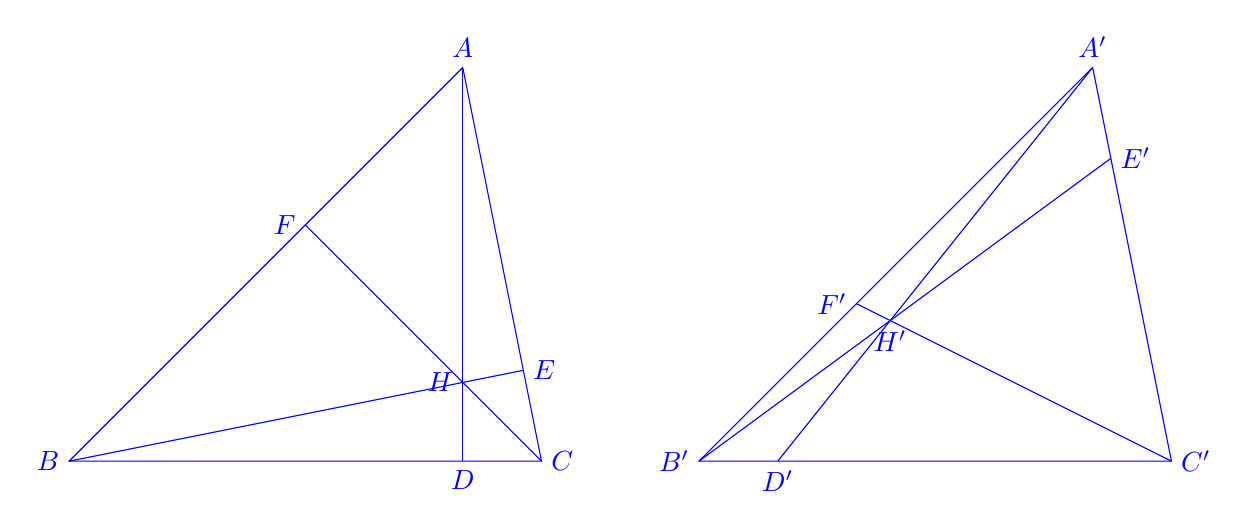
\begin{tikzpicture}
 \coordinate [label=above:\textcolor{blue}{$A$}] (A) at (5,5);
 \coordinate [label=left:\textcolor{blue}{$B$}] (B) at (0,0);
 \coordinate [label=right:\textcolor{blue}{$C$}] (C) at (6,0);
 \coordinate [label=below:\textcolor{blue}{$D$}] (D) at (5,0);
 \coordinate [label=left:\textcolor{blue}{$F$}](F) at (3,3);
 \coordinate [label=right:\textcolor{blue}{$E$}](E) at (150/26, 30/26);
 \coordinate [label=left:\textcolor{blue}{$H$}](H) at (5,1);
 
 \draw[blue] (A) -- (B) -- (C) -- (A);
 \draw[blue] (B) -- (E);
 \draw[blue] (C) -- (F);
 \draw[blue] (A) -- (D);
 
 \coordinate [label=above:\textcolor{blue}{$A'$}] (A') at (13,5);
 \coordinate [label=left:\textcolor{blue}{$B'$}] (B') at (8,0);
 \coordinate [label=right:\textcolor{blue}{$C'$}] (C') at (14,0);
 \coordinate [label=below:\textcolor{blue}{$D'$}] (D') at (9,0);
 \coordinate [label=left:\textcolor{blue}{$F'$}] (F') at (10,2);
 \coordinate [label=right:\textcolor{blue}{$E'$}] (E') at (172/13, 50/13);
 \coordinate [label=below:\textcolor{blue}{$H'$}] (H') at (73/7, 25/14);
 
  \draw[blue] (A') -- (B') -- (C') -- (A');
 \draw[blue] (B') -- (E');
 \draw[blue] (C') -- (F');
 \draw[blue] (A') -- (D');
\end{tikzpicture}
\ed

\bt{球面三角形余弦定理}{}
对于任给半径为$R$的球面三角形$\triangle ABC$, 其三边$a,b,c$和三角$\angle A, \angle B, \angle C$之间恒满足:
\begin{align*}
 \cos\frac{a}{R^2} & =\cos\frac{c}{R^2}\cos\frac{b}{R^2}+\sin\frac{b}{R^2}\sin\frac{c}{R^2}\cos\angle A,\\
 \cos\frac{b}{R^2} & =\cos\frac{a}{R^2}\cos\frac{c}{R^2}+\sin\frac{c}{R^2}\sin\frac{a}{R^2}\cos\angle B,\\
 \cos\frac{c}{R^2} & =\cos\frac{b}{R^2}\cos\frac{a}{R^2}+\sin\frac{a}{R^2}\sin\frac{b}{R^2}\cos\angle C.
\end{align*}
\et

\bt{球面三角形正弦定理}{}
条件同上, 有$\frac{\sin\angle A}{\sin\frac{a}{R^2}}=\frac{\sin\angle B}{\sin\frac{b}{R^2}}=\frac{\sin\angle C}{\sin\frac{c}{R^2}}$.
\et

\section{不等式集}
\bq{}{}
已知$0\le a_k\le 1$($k=1,2,\cdots, 2002$), 记$a_{2003}=a_1$, $a_{2004}=a_2$, 求$\sum_{k=1}^{2002}(a_k-a_{k+1}\cdot a_{k+2})$的最大值.
\eq
\ba
\bee
\sum_{k=1}^{2002}(a_k-a_{k+1}\cdot a_{k+2})=\sum_{k=1}^{2002}(a_k-a_{k}a_{k+1})=\sum_{k=1}^{2002}a_{k}(1-a_{k+1}).
\eee
Cauchy不等式, 上式右端不超过
\bee
\sqrt{\left(\sum_{k=1}^{2002}a_k^2\right)\left(\sum_{k=1}^{2002}(1-a_{k+1})^2\right)}
\le \frac{\sum a_k^2 + \sum (1-a_{k+1})^2}{2}
=\frac{\sum a_k^2+\sum(1-a_k)^2}{2}
=\frac{\sum(2a_k^2-2a_k+1)}{2}.
\eee
因为$2a_k^2-2a_k+1\le1$, 所以原式不超过$\frac12\sum1=1001$, 当$a_k=0$或$1$时取等号, 即当$a_1=a_3=a_5=\cdots=a_{2001}=1$且$a_2=a_4=\cdots=a_{2002}=0$时取等号.
\ea
\ba
由$0\le a_k\le 1$, 得$(1-a_k)(1-a_{k+1})=1-(a_{k}+a_{k+1})+a_{k}a_{k+1}\ge0$($k=1,2,\cdots, 2002$), 所以$1\ge a_{k}+a_{k+1}-a_{k}a_{k+1}\ge a_{k}+a_{k+1}-2a_{k}a_{k+1}$,
从而$2002\ge\sum_{k=1}^{2002}(a_k+a_{k+1}-2a_{k}a_{k+1})=2\sum(a_k-a_{k+1}a_{k+2})$, 即$\sum(a_k-a_{k+1}a_{k+2})\le1001$.
\ea

\bq{}{}
求函数$y=x+\sqrt{x(2-x)}$的最值及此时$x$的值.
\eq
\ba
显然$x\in[0,2]$, 所以可设$x=2\sin^2\theta$($\theta\in\mathbb{R}$), 运用$|a\sin\theta+b\cos\theta|\le\sqrt{a^2+b^2}$即可.
\ea

\bq{}{}
设$n$是给定的正整数, $n\ge13$, 对$n$个给定的实数$a_1, a_2, \cdots, a_n$, 记$|a_i-a_j|$($1\le i < j\le n$)有最小值$m$, 求在$\sum_{i=1}^{n}a_i^2=1$的条件下, 
$m$的最大值.
\eq
\ba
不妨设$a_1\le a_2\le \cdots\le a_n$, 于是$a_2-a_1\ge m, a_3-a_2\ge m, \cdots, a_n-a_{n-1}\ge m$, $a_j-a_i\ge(j-i)m$($1\le i< j \le n$).
\bee
\sum_{1\le i<j\le n}(a_i-a_j)^2\ge m^2\times\sum_{1\le i<j\le n}(j-i)^2
=m^2\sum_{k=1}^{n-1}k(2k+1)(k+1)=\frac{m^2}{12}\cdot n^2(n^2-1).
\eee
另一方面, $\sum_{i=1}^{n}a_i^2=1$可得
\bee
\sum_{1\le i<j\le n}(a_i-a_j)^2=n-\left(\sum_{i=1}^{n}a_i\right)^2\le n.
\eee
故$n\ge\frac{m^2}{12}n^2(n^2-1)$, 所以$m\le\sqrt{\frac{12}{n^2(n^2-1)}}$, 当且仅当$\sum_{i=1}^{n}a_i=0$,
且$a_1, a_2, \cdots, a_n$成等差数列时取等号.
\ea

\bq{}{}
若$x,y,z>0$且$x^2+y^2+z^2=1$, 则$S=\frac{(z+1)^2}{2xyz}$取最小值时, $x$的值是多少?
\eq
\ba
$\sqrt{\sqrt{2}-1}$.
\ea

\bl{}{}
设$T\ge0$, $x, y, z\ge0$, 则$T\ge\sum x$的充要条件为:
\begin{align}
 & (T^2-\sum x^2)^2-8\prod x\cdot T-4\sum y^2z^2\ge0\label{20170327001}\\
 & T^2\ge\sum x^2.\label{20170327002}
\end{align}
\el
\ba
若$T\ge\sum x$, 则\ref{20170327002}式明显成立, 且
\bee
(T+\sum x)(T^2-\sum x^2+2\sum yz)-8\prod x
\ge2\sum x\cdot 4\sum yz-8\prod x
\ge0.
\eee
根据
\be
(T^2-\sum x^2)^2-8\prod x\cdot T-4\sum y^2z^2
=(T-\sum x)\left[(T+\sum x)(T^2-\sum x^2+2\sum yz)-8\prod x\right]\label{20170327003}
\ee
知\ref{20170327001}式成立. 若\ref{20170327001}, \ref{20170327002}式成立, 则
\bee
(T+\sum x)(T^2-\sum x^2+2\sum yz)-8\prod x
\ge (\sqrt{\sum x^2}+\sum x)\cdot 2\sum yz-8\prod x
\ge (\sqrt{3}+3)(\prod x)^{\frac13}\cdot6(\prod x)^{\frac23}-8\prod x\ge0.
\eee
根据\ref{20170327003}式知$T\ge\sum x$.
\ea
由引理即得
\bt{}{20170328001}
设$T\ge0$, $x,y,z\ge0$, 记$f=(T^2-\sum x^2)^2-8\prod x\cdot T-4\sum y^2z^2$, 则
\begin{enumerate}[(i)]
 \item 若$f\ge0$, $\sum x^2\le T^2$, 则$\sum x\le T$;
 \item 若$f\le 0$, 则$\sum x\ge T$.
\end{enumerate}
\et

\bq{}{}
\bee
\sum\cos\frac{A}{2}\le2+\frac{s}{4R}+\frac{9\sqrt{3}-16}{4R}r.
\eee
\eq
\ba
设$m=\frac{s}{4R}$, $n=\frac{r}{2R}$. 则$\sum\cos^2\frac{A}{2}=2+n$, $\prod\cos\frac{A}{2}=\frac{m}{2}$. 进而
\bee
\sum\cos^2\frac{A}{2}\cos^2\frac{B}{2}=\frac14(4+4n+m^2+n^2).
\eee
令$T=2+\frac{m}{2}+\frac{9\sqrt{3}-16}{2}n$, $x=\cos\frac{A}{2}$, $y=\cos\frac{B}{2}$, $z=\cos\frac{C}{2}$,
用定理\ref{th:20170328001}中结论(i).
\ea

\bq{}{}
设实数$a,b,c,d$, 满足$a^2+b^2+c^2+d^2=5$, 求$(a-b)^2+(a-c)^2+(a-d)^2+(b-c)^2+(b-d)^2+(c-d)^2$的最大值.
\eq
\ba
设$f=(a-b)^2+(a-c)^2+(a-d)^2+(b-c)^2+(b-d)^2+(c-d)^2=15-2(ab+ac+ad+bc+bd+cd)+\lambda(a^2+b^2+c^2+d^2-5)$,
所以$f_a=-2(b+c+d)+2a\lambda$, $f_b=-2(a+c+d)+2b\lambda$, $f_c=-2(a+b+d)+2c\lambda$, $f_d=-2(a+c+d)+2b\lambda$,
$f_{\lambda}=a^2+b^2+c^2+d^2-5$, 令$f_a=f_b=f_c=f_d=f_{\lambda}=0$, 解得$\lambda=-1$或$a=b=c=d$.
当$\lambda=-1$时, $a+b+c+d=0$得$f=20$.
当$a=b=c=d$时, $f=0$, 所以$f_{\max}=20$.
\ea

\bq{}{}
如果$x>0$, $y>0$, $z>0$且$x^2+y^2+z^2=1$, 求$\frac{yz}{x}+\frac{xz}{y}+\frac{xy}{z}$的最小值.
\eq
\ba
设$\frac{yz}{x}=a$, $\frac{xz}{y}-b$, $\frac{xy}{z}=c$, 则
$ab+bc+ca=1$, 所以$a^2+b^2+c^2\ge ab+bc+ca=1$, 所以$(a+b+c)^2=a^2+b^2+c^2+2(ab+bc+ca)\ge3$,
另外令$f=a+b+c+\lambda(ab+bc+ca-1)$, 令
$f_a=1+(b+c)\lambda=0$, $f_b=1+(a+c)\lambda=0$, $f_c=1+(a+b)\lambda=0$, 所以
$a=b=c$时最小.
\ea

\bq{}{}
设$a_0, a_1, a_2, \cdots, a_n$满足$a_0=\frac12$, $a_{k+1}=a_k+\frac{1}{n}a_k^2$, $k=0,1,2,\cdots, n-1$,
其中$n$是一个给定的正整数, 试证: $1-\frac{1}{n}<a_n<1$.
\eq
\ba
$a_n>a_{n-1}>a_{n-2}>\cdots>a_2>a_1>a_0=\frac{1}{2}$,
\begin{align*}
 \frac{1}{a_k}-\frac{1}{a_{k+1}}=\frac{1}{n+a_k}<\frac{1}{n} \Longrightarrow\frac{1}{a_0}-\frac{1}{a_n}<1,\\
 \frac{1}{a_k}-\frac{1}{a_{k+1}}=\frac{1}{n+a_k}>\frac{1}{n+1} \Longrightarrow\frac{1}{a_0}-\frac{1}{a_n}>\frac{n}{n+1}.
\end{align*}
\ea

\bq{}{}
当$a>1$时, 若不等式$\frac{1}{n+1}+\frac{1}{n+2}+\cdots+\frac{1}{2n}>\frac{7}{12}\left[\log_{a+1}x-\log_{a}x+1\right]$对于不小于2的正整数$n$恒成立,
求$x$的取值范围.
\eq
\ba
$a_{n}=\frac{1}{n+1}+\frac{1}{n+2}+\cdots+\frac{1}{2n}$递增, $x$的取值范围为$(1, +\infty)$.
\ea

\bq{}{}
实数集$\{a_0, a_1, a_2, \cdots, a_n\}$, 满足以下条件: 
\begin{enumerate}[(1)]
 \item $a_1=a_n=0$.
 \item 对$1\le k\le n-1$, 有$a_k=c+\sum_{i=k}^{n-1}a_{i-k}(a_i+a_{i+1})$.
\end{enumerate}
证明: $c\le\frac{1}{4n}$.
\eq
\ba
定义$S_k=\sum_{i=0}^ka_i$($k=0,1,2,\cdots, n$), 则
\begin{align*}
 S_n
 & =\sum_{k=0}^{n}a_k
 =\sum_{k=0}^{n-1}a_{k-1}
 =nc+\sum_{k=0}^{n-1}\sum_{i=k}^{n-1}a_{i-k}(a_i+a_{i+1})\\
 & =nc+\sum_{i=0}^{n-1}(a_i+a_{i+1})\cdot\sum_{k=0}^{i}a_{i-k}\\
 & =nc+\sum_{i=0}^{n-1}(a_i+a_{i+1})\sum_{t=0}^{i}a_t, (t=i-k)\\
 & =nc+\sum_{i=0}^{n-1}(a_i+a_{i+1})\cdot S_i\\
 & =nc+\left[S_1S_0+(S_2-S_0)S_1+(S_3-S_1)S_2+\cdots+(S_n-S_{n-2})S_{n-1}\right]
\end{align*}
即$S_n^2-S_n+nc=0$, $\Delta\ge0\Longrightarrow c\le\frac{1}{4n}$.
\ea

\bq{}{}
若关于$x$的不等式$\log_{\frac{1}{a}}(\sqrt{x^2+ax+5}+1)\cdot\log_{5}(x^2+ax+6)+\frac{1}{\log_{3}a}\ge0$,
求$a$的取值范围.
\eq
\ba
令$u=x^2+ax+5$, $\frac{\log_3(\sqrt{u}+1)}{-\log_3a}\cdot\log_5(u+1)+\frac{1}{\log_3a}\ge0$.
因为$f(4)=1$, 所以$a=2$.
\ea

\bq{}{}
设$a_1, a_2, \cdots, a_{2002}>0$且$\sum\frac{1}{2+a_i}=\frac12$, 求$\prod a_i$的最小值.
\eq
\ba
令$x_i=\frac{2}{2+a_i}$, 则$\sum x_i=1$, 则$a_i=2\cdot\frac{1-x_i}{x_i}$, 
因为
\begin{align*}
 \prod a_i
 & =2^{2002}\prod\frac{1-x_i}{x_i}\\
 & =2^{2002}\cdot\frac{1}{x_1x_2\cdots x_{2002}}\prod(x_1+x_2+\cdots+x_{i-1}+x_{i+1}+\cdots+x_{2002})\\
 & \ge2^{2002}\cdot\frac{1}{x_ix_2\cdots x_{2002}}\cdot2001^{2002}\cdot\prod\sqrt[2001]{x_1x_2\cdots x_{i-1}x_{i+1}\cdots x_{2002}}\\
 &=4002^{2002}.
\end{align*}
\ea

\bq{}{}
求最小的正数$\lambda$, 使得对任意正整数$n$, $a_i$和$b_i$, $b_i\in[1,2]$($i=1,2,\cdots, n$), 且$\sum_{i=1}^{n}a_{i}^2=\sum b_i^2$, 
都有$\sum\frac{a_i^3}{b_i}\le\lambda\cdot\sum a_i^2$.
\eq
\ba
对任意$c_i, b_i\in[1,2]$, 有$\frac{1}{2}\le\frac{c_i}{b_i}\le 2$, 即$\frac{1}{2}b_i\le c_i\le2b_i$,
从而$\left(\frac{1}{2}b_i-c_i\right)(2b_i-c_i)\le0$, 即$c_i^2+b_i^2\le\frac{5}{2}c_ib_i$,
两边对$i$从1到$n$求和, 得$\sum c_i^2+\sum b_i^2\le\frac{5}{2}\sum c_ib_i$,
设$a_i, b_i\in\left[1, \frac{2}{3}\right]$, 因$a_i^2=\frac{a_i^{\frac{3}{2}}}{b_i^{\frac{1}{2}}}\cdot a_i^{\frac{1}{2}}\cdot b_i^{\frac{1}{2}}$.
又
\bee
\frac{1}{2}\le\frac{\frac{a_i^{\frac{3}{2}}}{b_{i}^{\frac{1}{2}}}}{a_i^{\frac{1}{2}}\cdot b_i^{\frac{1}{2}}}\le 2.
\eee
故有$\frac{5}{2}\sum a_i^2\ge\sum\frac{a_i^3}{b_i}+\sum a_ib_i\ge\sum\frac{a_i^3}{b_i}+\frac{2}{5}(\sum a_i^2+\sum b_i^2)=\sum\frac{a_i^3}{b_i}+\frac{4}{5}\sum a_i^2$,
即$\sum\frac{a_i^3}{b_i}\le\frac{17}{10}\sum a_i^2$, 当$n=2$, $a_1=1$, $a_2=2$, $b_1=2$, $b_2=1$时取等号.
\ea

\bq{}{}
已知: $x,y,z\in\mathbb{R}^*$, 有$xyz=1$且满足$x(1+z)>1$, $y(1+x)>1$, $z(1+y)>1$, 
求证: $2(x+y+z)\ge\frac{1}{x}+\frac{1}{y}+\frac{1}{z}+3$.
\eq
\ba
令$x=\frac{a}{b}$, $y=\frac{b}{c}$, $z=\frac{c}{a}$, 则$a+c>b$, $a+b>c$, $b+c>a$, 要证$2(x+y+z)\ge\frac1x+\frac1y+\frac1z+3$, 只需证
\bee
2\left(\frac{a}{b}+\frac{b}{c}+\frac{c}{a}\right)\ge\frac{b}{a}+\frac{c}{b}+\frac{a}{c}+3\Longleftrightarrow
  2(a^2c+b^2a+c^2b)\ge b^2c+c^2a+a^2b+3abc.
\eee
因为
\bee
(a+b-c)(b-c)^2\ge0, \quad (b+c-a)(c-a)^2\ge0, \quad (c+a-b)(a-b)^2\ge0
\eee
展开相加, 即得.
\ea

\bq{}{}
已知正整数$n\ge 2$, 若对同时满足条件:
\begin{enumerate}[(1)]
 \item $a_1a_2\cdots a_n=b_1 b_2\cdots b_n$;
 \item $\sum_{1\le i<j\le n}|a_i-a_j|\le \sum_{1\le i<j\le n}|b_i-b_j|$的任意正数$a_1,\cdots, a_n$与$b_1,\cdots, b_n$,
 总有$\sum_{i=1}^{n}a_i\le\lambda\sum_{i=1}^{n}b_i$. 试求正数$\lambda$的最小值.
\end{enumerate}
\eq
\ba
一方面, 取$(a_1,\cdots, a_n)=(1,1,\cdots,(1+x)x^{n-1})$, $(b_1,\cdots,b_n)=(1+x,x,x,\cdots, x)$, 满足(1)与(2), 
此时$\lambda\ge\frac{\sum a_i}{\sum b_i}=\frac{n-1+x^{n-1}+x^n}{1+nx}$, 令$x\to0$, 则$\lambda\ge n-1$.

以下证明$\lambda=n-1$时, 不等式成立.

不妨设$a_1\ge a_2\ge\cdots\ge a_n$, $b_1\ge b_2\ge \cdots\ge b_n$, $n=2$时, 显然成立.

设$n\ge3$,

(1) 若$a_1\le\frac{n-1}{n}b_1$, 则$\sum a_i\le na_1\le(n-1)b_1\le(n-1)\sum b_i$.

(2) 若$a_1>\frac{n-1}{n}b_1$, 则
\begin{align*}
 2(b_2+\cdots+b_n) & \ge 2(n-1)\cdot(b_2\cdots b_n)^{\frac{1}{n-1}}=2(n-1)\left(\frac{a_1}{b_1}a_2\cdots a_n\right)^{\frac{1}{n-1}}\\
  & \ge 2(n-1)\left(\frac{a_1}{b_1}\right)^{\frac{1}{n-1}}\cdot a_n>2(n-1)\cdot\left(\frac{n-1}{n}\right)^{\frac{1}{n-1}}\cdot a_n\\
  & \ge na_n.
\end{align*}
所以
\begin{align*}
 (n-1)\sum b_i &= (n-1)b_1+(n-3)\sum_{i=2}^{n}b_i+2\sum_{i=2}^{n}b_i\\
  &\ge(n-1)b_1+(n-3)\sum_{i=2}^{n}b_i+na_n\ge[(n-1)b_1+(n-3)b_2+\cdots-(n-1)b_n]+na_n\\
  &=\sum_{1\le i<j\le n}|b_i-b_j|+na_n\ge\sum_{1\le i<j\le n}|a_i-a_j|+na_n\\
  &=[(n-1)a_1+(n-3)a_2+\cdots-(n-1)a_n]+na_n\\
  &\ge(n-1)a_1+a_n\ge a_1+a_2+\cdots+a_{n-1}+a_n.
\end{align*}
\ea

\bq{1998年上海市高中数学竞赛}{}
设非零多项式$f(x)=a_nx^n+a_{n-1}x^{n-1}+\cdots+a_0$, $g(x)=c_{n+1}x^{n+1}+c_nx^n+\cdots+c_0$, 满足$g(x)=(x+r)f(x)$, 其中$r$为一实数,
设$a=\max(|a_{n}|, |a_{n-1}|,\cdots,|a_0|)$, $c=\max(|c_{n+1}|,|c_{n}|,\cdots,|c_0|)$, 求证: $\frac{a}{c}\le n+1$.
\eq
\ba
设$|r|\le1$, 由$\sum_{i=0}^{n+1}c_ix^i=(x+r)\sum_{i=0}^{n}a_ix^i=a_nx^{n+1}+\sum_{i=1}^{n}(ra_i+a_{i-1})x^i+ra_0$. 
故
\bee
\begin{dcases}
 c_{n+1}=a_n\\
 c_{n}=ra_n+a_{n-1}\\
 \cdots\\
 c_{1}=ra_1+a_0\\
 c_0=ra_0
\end{dcases}
\Longrightarrow
\begin{dcases}
 a_{n}=c_{n+1}\\
 a_{n-1}=-rc_{n+1}+c_n\\
 a_{n-2}=(-r)^2c_{n+1}+(-r)c_n+c_{n-1}\\
 \cdots\\
 a_0=(-r)^nc_{n+1}+(-r)^{n-1}c_n+\cdots+c_1,
\end{dcases}
\eee
故$|a|=|a_i|=|(-r)^{n-i}c_{n+1}+\cdots+c_{i+1}|\le|c_{n+1}|+\cdots+|c_{i+1}|\le(n-i+1)c\le(n+1)c$.

如果$|r|>1$, 令$x=\frac{1}{x}$, 代入$g(x)=(x+r)f(x)$, 则转化为上述情形, 仍有$a\le(n+1)c$.

另外
\bee
  |a|=|a_i|\le|r|^{n-i}|c_{n+1}|+\cdots+|c_{i+1}|\le(|r^n|+|r^{n-1}|+\cdots+1)c\le\frac{|r|^{n+1}-1}{|r|-1}c
\eee
而
\bee
\frac{|r|^{n+1}-1}{|r|-1}\le n+1
\Longleftrightarrow |r|^{n+1}\ge n|r|-n+|r|
\Longleftrightarrow |r|^n+\frac{n}{|r|}\ge n+1
\Longleftrightarrow |r|^n+\frac{1}{|r|}+\cdots+\frac{1}{|r|}\ge n+1
\eee

($|r|=0$时, 命题显然成立).
\ea

\bq{}{}
若$a,b,c\in\mathbb{R}$, 且$5a^4+4b^4+6c^4=90$, 求$5a^3+2b^3+3c^3$的最大值.
\eq
\ba
只需考虑$a,b,c\in\mathbb{R}^*$. 因$a^3=\frac12(a\cdot a\cdot a\cdot2)\le\frac{1}{8}(a^4+a^4+a^4+2^4)=\frac38a^4+2$,
同理$b^3\le\frac34b^4+\frac14$, $c^3\le\frac34c^4+\frac14$, 所以所求最大值为$45$.
\ea

\bq{}{}
若$x,y,z$为实数, $0<x<y<z<\frac{\pi}{2}$, 证明: $\frac{\pi}{2}+2\sin x\cos y+2\sin y\cos z>\sin 2x+\sin 2y+\sin 2z$.
\eq
\ba
原不等式等价于证明$\frac{\pi}{4}>\sin x(\cos x-\cos y)+\sin y(\cos y-\cos z)+\sin z\cos z$. 如图所示
\begin{center}
 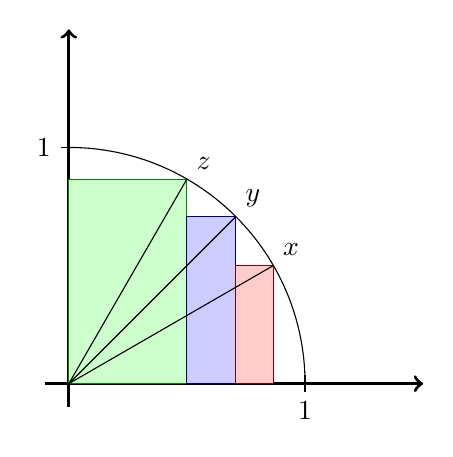
\begin{tikzpicture}[scale=3]
  \draw[->,very thick] (-.1,0) -- (1.5,0) coordinate (x axis);
  \draw[->,very thick] (0,-0.1) -- (0,1.5) coordinate (y axis);
  \draw (1,0) arc [start angle=0,end angle=90,x radius=1cm,y radius=1cm];
  let x=30;
  let y=45;
  let z=60;
  \filldraw[fill=green!20, draw=green!50!black] (0,0) -- (0.5,0) -- (0.5,0.866) -- (0,0.866) -- cycle;
  \filldraw[fill=blue!20, draw=blue!50!black] (0.5,0) -- (0.707,0) -- (0.707,0.707) -- (0.5,0.707) -- cycle;
  \filldraw[fill=red!20, draw=red!50!black] (0.707,0) -- (0.866,0) -- (0.866,0.5) -- (0.707,0.5) -- cycle;
  \draw (0,0) -- (0.866,0.5) node [anchor=south west] {$x$};
  \draw (0,0) -- (0.707,0.707) node [anchor=south west] {$y$};
  \draw (0,0) -- (0.5,0.866) node [anchor=south west] {$z$};
  \draw (1,1pt) -- (1,-1pt) node [anchor=north] {$1$};
  \draw (1pt,1) -- (-1pt,1) node [anchor=east] {$1$};
  \end{tikzpicture}
\end{center}
\ea

\bq{1987年第21届全苏MO}{}
正数$a,b,c,A,B,C$满足条件$a+A=b+B=c+C=k$, 求证: $aB+bC+cA<k^2$.
\eq
\ba
主试委员会给出的解答是$k^3=(a+A)(b+B)(c+C)$, 利用放缩的技巧给出证明, 北京四中的袁峰同学给出了如下构造性证明.

如图: $S_{\triangle LRM}+S_{\triangle PNM}+S_{\triangle QLN}<S_{\triangle PQR}$, 化简即得.
\begin{center}
 \begin{tikzpicture}[scale=3]
  \coordinate [label=left:$Q$] (Q) at (0,0);
  \coordinate [label=above:$P$] (P) at (0.5,0.866);
  \coordinate [label=right:$R$] (R) at (1,0);
  \draw (P) -- (Q) -- (R) -- cycle;
  \coordinate [label=below:$L$] (L) at ($ (R) !0.7! (Q) $);
  \coordinate [label=right:$M$] (M) at ($ (P) !0.4! (R)$);
  \coordinate [label=left:$N$] (N) at ($ (P) !0.5! (Q)$);
  \draw (L) -- (M) -- (N) -- cycle;
  \node (A) [label=below:$A$] at ($ (Q) !0.5! (L) $) {};
  \node (a) [label=below:$a$] at ($ (R) !0.5! (L) $) {};
  \node (B) [label=right:$B$] at ($ (M) !0.5! (R) $) {};
  \node (b) [label=right:$b$] at ($ (P) !0.5! (M) $) {};
  \node (C) [label=left:$C$] at ($ (P) !0.5! (N) $) {};
  \node (c) [label=left:$c$] at ($ (N) !0.5! (Q) $) {};
  
  \foreach \point in {P,Q,R,L,M,N}
    \fill [blue,opacity=.75] (\point) circle (1pt);
 \end{tikzpicture}

\end{center}

\ea
\ba
如图:
\begin{center}
 \begin{tikzpicture}[scale=3]
  \coordinate[label=225:$P$] (P) at (0,0);
  \coordinate[label=315:$Q$] (Q) at (1,0);
  \coordinate[label=45:$R$] (R) at (1,1);
  \coordinate[label=135:$S$] (S) at (0,1);
  
  \draw (P) -- (Q) -- (R) -- (S) -- cycle;
  \filldraw[fill=yellow!80!black,opacity=0.5] (P) rectangle (0.6,0.4);
  \filldraw[fill=red!80!black,opacity=0.5] (0.6,0) rectangle (1,0.7);
  \filldraw[fill=blue!80!black,opacity=0.5] (1,0.7) rectangle (0.3,1);
  
  \node [label=below:$B$] at ( $ (P) !0.5! (0.6,0) $) {};
  \node [label=below:$b$] at ( $ (Q) !0.5! (0.6,0) $) {};
  \node [label=right:$C$] at ( $ (Q) !0.5! (1,0.7) $) {};
  \node [label=right:$c$] at ( $ (R) !0.5! (1,0.7) $) {};
  \node [label=above:$A$] at ( $ (R) !0.5! (0.3,1) $) {};
  \node [label=left:$a$] at ( $ (P) !0.5! (0,0.4) $) {};
  
  \foreach \point in {P,Q,R,S}
    \fill [blue,opacity=.75] (\point) circle (1pt);
 \end{tikzpicture}

\end{center}

\ea

\bq{第31届IMO预选题}{}
设集合$\{a_1,a_2,\cdots,a_n\}=\{1,2,\cdots,n\}$, 求证:
\bee
\frac12+\frac23+\cdots+\frac{n-1}{n}\le\frac{a_1}{a_2}+\frac{a_2}{a_3}+\cdots+\frac{a_{n-1}}{a_n}.
\eee
\eq
\ba
设$b_1,b_2,\cdots,b_{n-1}$是$a_1,a_2,\cdots,a_{n-1}$的一个排列, 且$b_1<b_2<\cdots<b_{n-1}$, 
$c_1,c_2,\cdots,c_{n-1}$是$a_2,a_3,\cdots,a_{n}$的一个排列, 且$c_1<c_2<\cdots<c_{n-1}$, 则
\bee
\frac1{c_1}>\frac1{c_2}>\cdots>\frac1{c_{n-1}}.
\eee
且$b_1\ge1$, $b_2\ge2$, $\cdots,b_{n-1}\ge n-1$, $c_1\le 2,c_2\le3,\cdots,c_{n-1}\le n$,
由排序不等式得:
\bee
\frac{a_1}{a_2}+\frac{a_2}{a_3}+\cdots+\frac{a_{n-1}}{a_n}
  \ge \frac{b_1}{c_1}+\frac{b_2}{c_2}+\cdots+\frac{b_{n-1}}{c_{n-1}}
  \ge \frac12+\frac23+\cdots+\frac{n-1}{n}.
\eee
这是南斯拉夫提给第31届IMO的一道试题, 原证法是利用加强命题的手法, 用数学归纳法给出证明.
一则加强命题很难想到, 二则归纳法证明要对足标进行讨论, 比较麻烦. 在当年国家集训队里姚建钢同学(第35届IMO金牌得主)的证法,
更是干脆, 漂亮, 出人意料.
\ea
\ba
易证
\bee
\prod_{k=1}^{n-1}(a_k+1)\ge\prod_{k=1}^na_k,
\eee
故
\begin{align*}
 \sum_{k=1}^{n-1}\frac{a_k}{a_{k+1}}+\paren{\sum_{k=1}^n\frac1k}
  &=\frac{1}{a_1}+\sum_{k=1}^{n-1}\frac{a_k+1}{a_{k+1}}\\
  &\ge n \sqrt[n]{\frac{\prod_{k=1}^{n-1}(a_k+1)}{\prod_{k=1}^na_k}}\ge n\\
  &=\sum_{k=1}^{n}\frac{1}{k}+\sum_{k=1}^{n-1}\frac{k}{k+1}
\end{align*}

\ea

\bq{第24届IMO}{}
设$a,b,c$分别为一个三角形的三边之长, 求证:
\bee
a^2b(a-b)+b^2c(b-c)+c^2a(c-a)\ge0.
\eee
并指出等号成立的条件.
\eq
\ba
原联邦德国选手伯恩哈德$\cdot$里普只用了一个等式:
\bee
a^2b(a-b)+b^2c(b-c)+c^2a(c-a)
  = a(b-c)^2(b+c-a)+b(a-b)(a-c)(a+b-c)
\eee
由轮换对称性, 不妨设$a\ge b, c$, 即得欲证不等式成立, 而且显然等号成立的充要条件是$a=b=c$.

里普的证法新颖, 巧妙, 简洁, 与主试委员会提供的参考答案不同, 他因此获得了该届的特别奖.
\ea

\bq{1980年芬兰, 英国, 匈牙利, 瑞典四国联赛}{}
设数列$a_0,a_1,\cdots,a_n$满足$a_0=\frac12$及$a_{k+1}=a_k+\frac1na_k^2$($k=0,1,2,\cdots,n-1$),
其中$n$是一个给定的正整数, 试证:
\bee
1-\frac1n<a_n<1.
\eee
\eq
\ba
该题是该次竞赛得分率最低的一道试题, 主试委员会所给出的解法也相当繁琐, 前后共用了四次归纳法, 译成中文后有4000多字,
中国科技大学白志东先生对此题采用了大胆的处理方法, 加强命题, 出奇制胜给出一个简洁的证明.

由于$a_1=a_0+\frac1na_0^2=\frac12+\frac1{4n}=\frac{2n+1}{4n}$, 所以
\bee
\frac{n+1}{2n+1}<a_1<\frac{n}{2n-1}.
\eee
我们来用归纳法证: 对于一切$1\le k\le n$, 都有
\be\label{20180704001}
\frac{n+1}{2n-k+2}<a_k<\frac{n}{2n-k}.
\ee
假设(\ref{20180704001})对于$k<n$成立, 则
\bee
a_{k+1}=a_k\paren{1+\frac1na_k}
  <\frac{n}{2n-k}\paren{1+\frac1{2n-k}}
  =\frac{n(2n-k+1)}{(2n-k)^2}
  <\frac{n}{2n-(k+1)}.
\eee
所以
\begin{align*}
 a_{k+1} & = a_k+\frac1na_k^2>\frac{n+1}{2n-k+2}+\frac{(n+1)^2}{n(2n-k+2)^2}\\
  &>\frac{n+1}{2n-(k+1)+2}
\end{align*}
于是(\ref{20180704001})式对于一切$1\le k\le n$均成立, 特别在$k=n$时,
\bee
1-\frac1n<\frac{n+1}{n+2}<a_n<\frac{n}{n}=1.
\eee

{\bf{说明}} 这里所证的不等式(\ref{20180704001})式比题目所要证明的不等式强, 却收到了事半功倍之效,
下面给出一种直接了当的证明.
\ea
\ba
由已知, 
\bee
\frac1{a_{k-1}}-\frac1{a_k}=\frac1{n+a_{k-1}},
\eee
从而$a_n>a_{n-1}>\cdots>a_1>a_0=\frac12$. 所以
\bee
\frac1{a_{k-1}}-\frac1{a_k}<\frac1n,\quad k=1,2,\cdots,n.
\eee
累加得$\frac1{a_0}-\frac1{a_n}>\frac{n}{n+1}$, 所以$\frac{1}{a_n}<2-\frac{n}{n+1}=\frac{n+2}{n+1}$.
\ea

\bq{}{}
已知函数$f(x)$的定义域为$\Reals$, 对于任意实数$m,n$均有$f(m+n)=f(m)+f(n)-1$, 且$f\paren{\frac12}=2$, 
当$x>-\frac12$时, 恒有$f(x)>0$, 求证: $f(x)$单调递增.
\eq
\ba
证明: 令$x_1>x_2$, 所以
\bee
f(x_1)-f(x_2)=f(x_1-x_2)-1
  =f\paren{\paren{x_1-x_2-\frac12}+\frac12}-1
  =f\paren{x_1-x_2-\frac12}+f\paren{\frac12}-1-1
  =f\paren{x_1-x_2-\frac12}
\eee
因为$x_1-x_2-\frac12>-\frac12$, 所以$f\paren{x_1-x_2-\frac12}>0$, 
所以$f(x_1)>f(x_2)$, 得证.
\ea

\bq{}{}
已知: 正数$x,y,z$均小于$1$且$x+y+z=2$, $w=xy+yz+zx$, 求$w$的取值范围.
\eq
\ba
易得$w\le\frac43$, 令$x(1-x)=a^2$, $y(1-y)=b^2$, $z(1-z)=c^2$, 因为
\bee
w=xy+z(2-z)=xz+y(2-y)=yz+x(2-x)
\eee
所以
\bee
3w=w+2\times2-x^2-y^2-z^2=w+4+a^2+b^2+c^2-2
\eee
所以$2w=2+a^2+b^2+c^2\ge2$, 即$w\ge1$.
仅当$a,b,c=0$时取$w=1$, 但$a,b,c\ne0$, 所以$w>1$.
\ea

\bq{}{}
已知$\frac{a^2+b^2}{4}+c^2=1$, 求$a+b+c$的最大值.
\eq
\ba
\begin{align*}
 (a+b+c)^2 = & a^2+b^2+c^2+2bc+2ab+2ac\\
  \le & a^2+b^2+c^2+(a^2+b^2)+\paren{\frac{b^2}{4}+4c^2}+\paren{\frac{a^2}{4}+4c^2}\\
  = & 9\paren{\frac{a^2+b^2}{4}}=9.
\end{align*}
\ea

\bq{}{}
已知$a,b>0$, $a+b=1$, 证明: $\frac32<\frac1{a^2+1}+\frac1{b^2+1}\le\frac85$.
\eq
\ba
原式等价于证明:
\begin{align*}
 15(a^2+1)(b^2+1)<10(a^2+b^2+2)\le16(a^2+1)(b^2+1)
  & \Longleftrightarrow 15a^2b^2+5a^2+5b^2-5<0\le16a^2b^2+6a^2+6b^2-4\\
  & \Longleftrightarrow 3a^2b^2+a^2+b^2-1<0\le8a^2b^2+3a^2+3b^2-2.
\end{align*}
因$a+b=1$, 所以$a^2+b^2-1=-2ab$. 所以上式等价于
\bee
3a^2b^2-2ab<0\le8a^2b^2-6ab+1.
\eee
又由$a^2+b^2+2ab=1\ge4ab$, 所以$0<ab\le\frac14$, 所以上式成立.
\ea
\ba
令$a=\sin^2\theta, b=\cos^2\theta$, $\paren{0<\theta<\frac{\pi}{2}}$, 所以
\begin{align*}
\frac1{a^2+1}+\frac1{b^2+1}
  &=\frac1{1+\sin^4\theta}+\frac1{1+\cos^4\theta}\\
  &=\frac4{5-2\cos2\theta+\cos^22\theta}+\frac4{5+2\cos2\theta+\cos^22\theta}\\
  &=\frac{16(11+\cos4\theta)}{(11+\cos4\theta)^2-8(11+\cos4\theta)+80}\\
  &=\frac{16y}{y^2-8y+80}=\frac{16}{y+\frac{80}{y}-8}
\end{align*}
因$0<\theta<\frac{\pi}{2}$, 所以$0<4\theta<2\pi$. 所以$10<y\le12$, 并有$\frac32<\frac{16}{y+\frac{80}{y}-8}\le\frac85$.
\ea

\bq{}{}
已知数列$\{a_n\}$, $\{b_n\}$, $\{c_n\}$满足: $b_n=a_n-a_{n+2}$, $c_n=a_n+2a_{n+1}+3a_{n+2}$, ($n=1,2,3,\cdots$),
若$\{c_n\}$为等差数列且$b_n\le b_{n+1}$, 证明: $b_n=b_{n+1}$.
\eq
\ba
由于$a_n-a_{n+2}=b_{n}\le b_{n+1}\le b_{n+2}=a_{n+2}-a_{n+4}$, 所以$2a_{n+2}\ge a_n+a_{n+4}$.
因为$2c_{n+1}=c_n+c_{n+2}$, 所以$4a_{n+3}=a_{n}+3a_{n+4}\le 2a_{n+2}+2a_{n+4}$, 
所以$2a_{n+3}\le a_{n+2}+a_{n+4}$. 所以$a_{n+3}-a_{n+2}\le a_{n+4}-a_{n+3}\le a_{n+5}-a_{n+4}$, 
所以$a_{n+3}-a_{n+5}\le a_{n+2}-a_{n+4}$, 所以$b_{n+3}\le b_{n+2}\le b_{n+3}$,
所以$b_{n+3}=b_{n+2}$, ($n\ge1$). 所以$b_3=b_4=b_5=\cdots=-2d=a_3-a_5=a_4-a_6=a_5-a_7$, 
所以
\begin{align*}
 4a_5-3a_6=a_2\le a_3-a_5+a_4
 &\Longrightarrow 5a_5\le a_3+a_4+3a_6\\
 &\Longrightarrow 5(a_3+2d)\le a_3+a_4+3(a_4+2d)\\
 &\Longrightarrow 2a_3\le2a_4-2d=2a_4+a_3-a_5\\
 &\Longrightarrow a_3+a_5\le 2a_4.
\end{align*}
因$a_3+a_5\ge2a_4$, 所以$a_2=a_3-a_5+a_4$, 同理$a_1=a_2-a_4+a_3$,
即$b_1=b_2=b_3=\cdots$.

两个正数$a,b$的和一定时, 它们的积
\be
ab=\frac14\paren{(a+b)^2-(a-b)^2}
\ee
随着差$\abs{a-b}$的增大而减小;
其平方和
\be
a^2+b^2=\frac12\paren{(a+b)^2+(a-b)^2}
\ee
随着差$\abs{a-b}$的增大而增大.
\ea

\bq{}{}
已知$\triangle ABC$的三边, $a, b,c$成等比数列, 则$\sin B+\cos B$的取值范围为\underline{$\qquad$}.
\eq
\ba
命题等价于$a+b>c$, $a+c>b$, $b+c>a$, $b^2=ac$,
\bee
b^2=ac=a^2+c^2-2ac\cos B\ge2ac-2ac\cos B,
\eee
所以$\cos B\ge\frac12$, $0<B\le60^{\circ}$, 由$\frac12\le\cos B<1$及$0<\sin B\le\frac{\sqrt{3}}{2}$,
所以
\be\label{20180705001}
\frac12<\cos B+\sin B<\frac{\sqrt{3}}{2}+1,
\ee
另一方面, $\sin B+\cos B=\sqrt{2}\sin(B+45^{\circ})$, 而$45^{\circ}<B+45^{\circ}<105^{\circ}$,
故
\be\label{20180705002}
1<\sin B+\cos B\le \sqrt{2}.
\ee
综合(\ref{20180705001}), (\ref{20180705002})有$1<\sin B+\cos B\le\sqrt{2}$.
\ea

\bq{}{}
设$a,b,c$是直角$\triangle ABC$的三边长, $c$为斜边, 求使不等式
\bee
a^2(b+c)+b^2(c+a)+c^2(a+b)\ge kabc
\eee
恒成立的$k$的最大值.
\eq
\ba
$a>0, b>0, c>0$, $c^2=a^2+b^2$, 所以
\begin{align*}
 LHS&=(a^2+b^2)c+a\paren{b^2+\frac{c^2}{2}}+b\paren{\frac{c^2}{2}+a^2}+\frac{c}{2}\cdot c(a+b)\\
  &\ge 2abc+\sqrt{2}abc+\sqrt{2}abc+\frac{c}{2}\sqrt{a^2+b^2}\cdot2\sqrt{ab}\\
  &\ge (2+2\sqrt{2})abc+c\cdot\sqrt{2ab}\cdot\sqrt{ab}=(2+3\sqrt{2})abc,
\end{align*}
仅当$a=b$时上式取等号.
\bee
(a+b+c)\paren{\frac1a+\frac1b+\frac1c}\ge5+3\sqrt{2}.
\eee
\ea

\bq{}{}
设$x_1$是方程$\sqrt{3}\sin x-3\cos x=2a-1$的最大负根, $x_2$是方程$2\cos^2 x-2\sin^2x=a$的最小正根,
求使不等式$\abs{x_1}\le x_2$成立的实数$a$的取值范围.
\eq
\ba
方程$\sqrt{3}\sin x-3\cos x=2a-1$等价于$\sin\paren{x-\frac{\pi}{3}}=\frac{2a-1}{2\sqrt{3}}$, 
从而得到$-1\le \frac{2a-1}{2\sqrt{3}}\le 1$. 解得$\frac12-\sqrt{3}\le a\le \frac12+\sqrt{3}$, 而且
\bee
x_1=\left\{
\begin{array}{ll}
 \frac{\pi}{3}+\arcsin\frac{2a-1}{2\sqrt{3}}, & \paren{\frac12-\sqrt{3}\le a<-1}\\
 -\frac{2\pi}{3}-\arcsin\frac{2a-1}{2\sqrt{3}}, & \paren{-1\le a\le\frac12+\sqrt{3}}
\end{array}
\right.
\eee
其图像如图, 位于$a$轴下方, 方程$2\cos^2x-2\sin^2x=a$等价于$\cos 2x=\frac{a}{2}$,
其中$-1\le\frac{a}{2}\le 1$, 所以$-2\le a\le 2$, 解得
\bee
x_2=\left\{
\begin{array}{ll}
 \frac12\arccos\frac{a}{2}, & (-2<a\le 2)\\
 \pi, & (a=2).
\end{array}
\right.
\eee
其图像如图, 它位于$a$轴上方, 比较两个函数的图像, 不难看出$|x_1|\le x_2$的充要条件是$\frac12-\sqrt{3}\le a\le -1$或$a=2$.
\begin{center}
 \begin{tikzpicture}
  \begin{axis}[
    axis equal,
    axis lines=middle,
    axis line style={->},
    xlabel={$a$},
    ylabel={$x$},
    ]
   \addplot[blue,thick] gnuplot [domain=-1.232:-1,samples=120] {pi/3+asin((2*x-1)/(2*sqrt(3)))};
   \addplot[blue,thick] gnuplot [domain=-1:2.232,samples=120] {-2*pi/3-asin((2*x-1)/(2*sqrt(3)))};
   \addplot[blue,thick] gnuplot [domain=-2:2,unbounded coords=jump,samples=120] {0.5*acos(x/2)};
   \addplot[
    scatter,
    only marks,
    nodes near coords,
    point meta=explicit symbolic,
    scatter/classes={
      o={mark=*,fill=white},
      c={mark=*,blue}},
   ] table[meta=label] {
      x		y	label
      2	3.14	c
      2	0	o
      -2	1.57	c
      -1	0	o
      -1.232	-0.52	c
      -1	-1.04	c
      2.232	-3.66	c
    };
    \addplot [name path=border,color=blue, ultra thick, dashed] coordinates {(2,0) (2,3.14) (0,3.14)};
    \addplot [name path=border,color=blue, ultra thick, dashed] coordinates {(-2,0) (-2,1.57) (0,1.57)};
    \addplot [name path=border,color=blue, ultra thick, dashed] coordinates {(-1.232,0) (-1.232,-0.52) (0,-0.52)};
    \addplot [name path=border,color=blue, ultra thick, dashed] coordinates {(-1,0) (-1,-1.04) (0,-1.04)};
    \addplot [name path=border,color=blue, ultra thick, dashed] coordinates {(2.232,0) (2.232,-3.66) (0,-3.66)};
    \addplot+[only marks,nodes near coords,blue,point meta=explicit symbolic] coordinates {
      (-2,1.57) [$(-2,\frac{\pi}{2})$]
      (2,3.14) [$(2,\pi)$]
    };
  \end{axis}
 \end{tikzpicture}
\end{center}
\ea

\bq{}{}
函数$y=\sqrt{8x-x^2}-\sqrt{14x-x^2-48}$的最大值为\underline{$2\sqrt{3}$}, 最小值为\underline{0}.
\eq
\ba
$x$的定义域为$6\le x \le 8$, 而
\bee
f(x)=\frac{6\sqrt{8-x}}{\sqrt{x}+\sqrt{x-6}}
\eee
在$[6,8]$上递减.
\ea

\bq{}{}
已知$a,b,c,d\in\Reals$, 满足$a+b+c+d=3$, $a^2+2b^2+3c^2+6d^2=5$, 
则$a$的最小值与最大值的和是\underline{3}.
\eq
\ba
\bee
5-a^2=2b^2+3c^2+6d^2=\frac16(3+2+1)(2b^2+3c^2+6d^2)\ge(b+c+d)^2=(3-a)^2.
\eee
\ea

\bq{}{}
用$\delta(S)$表示非零整数集$S$中所有元素的和, 设$A=\{a_1,a_2,\cdots,a_{11}\}$是正整数集,
且$a_1<a_2<\cdots<a_{11}$, 若对每个正整数$n\le1500$, 存在$A$的子集$S$, 使得$\delta(S)=n$,
求满足上述要求的$a_{10}$的最小值.
\eq
\ba
令$S_k=a_1+a_2+\cdots+a_k$, ($1\le k\le 11$), 若$a_k>S_{k-1}+1$,
则不存在$S\subset A$, 使$\delta(S)=S_{k-1}+1$, 所以$S_k=S_{k-1}+a_k\le2S_{k-1}+1$.
又由题设得$S_1=a_1=1$, 于是由归纳法易得$S_k\le2^k-1$, ($1\le k\le m$).
若$S_{10}<750$, 则$a_{11}\le750$, (否则$750$无法用$\delta(S)$表出),
$S_{11}=S_{10}+a_{11}<1500$, 所以$S_{10}\ge750$.
又$S_{8}\le2^8-1=255$, 所以$2a_{10}\ge a_{9}+a_{10}=S_{10}-S_8\ge495$,
$a_{10}\ge248$, 另一方面, 令$A=\{1,2,4,8,16,32,64,128,247,248,750\}$合题意.
\ea

\bq{}{}
$a,b,c>0$, $l^2=a^2+b^2+c^2$, 证明: $(l^4-a^4)(l^4-b^4)(l^4-c^4)\ge512a^4b^4c^4$.
\eq
\ba
\begin{align*}
 LHS & = (l^2+a^2)(l^2+b^2)(l^2+c^2)(l^2-a^2)(l^2-b^2)(l^2-c^2)\\
  &=(2a^2+b^2+c^2)(a^2+2b^2+c^2)(a^2+b^2+2c^2)(b^2+c^2)(c^2+a^2)(a^2+b^2)\\
  &\ge 4\sqrt[4]{a^4b^2c^2}\cdot4\sqrt[4]{a^2b^4c^2}\cdot4\sqrt[4]{a^2b^2c^4}\cdot2\sqrt{b^2c^2}\cdot2\sqrt{c^2a^2}\cdot2\sqrt{a^2b^2}\\
  &=RHS.
\end{align*}
\ea
\ba
问题等价于证明
\bee
\paren{\frac{l^4}{a^4}-1}\paren{\frac{l^4}{b^4}-1}\paren{\frac{l^4}{c^4}-1}\ge512
\eee
设$x=\frac{a^2}{l^2}$, $y=\frac{b^2}{l^2}$, $z=\frac{c^2}{l^2}$, 则$x+y+z=1$, 所以上式等价于证明
\bee
\paren{\frac1{x^2}-1}\paren{\frac1{y^2}-1}\paren{\frac1{z^2}-1}\ge512.
\eee
因
\bee
\frac{1}{x^2}-1=\frac{(1-x)(1+x)}{x^2}=\frac{(y+z)(x+y+z+x)}{x^2}
  \ge\frac{2\sqrt{yz}(2x+2\sqrt{yz})}{x^2}
  \ge\frac{2\sqrt{yz}\cdot4\sqrt{x\sqrt{yz}}}{x^2}
  =\frac{8\sqrt[4]{x^2y^3z^3}}{x^2}.
\eee
等号当且仅当$x=y=z$时取得, 同理$\frac1{y^2}-1\ge8\frac{\sqrt[4]{x^3y^2z^3}}{y^2}$, 
$\frac{1}{z^2}-1\ge8\frac{\sqrt[4]{x^3y^3z^2}}{z^2}$, 以上三式相乘即得.
\ea

\bq{}{}
在锐角$\triangle ABC$中, $a<b<c$, 记$P=\frac{a+b+c}{2}$, $Q=a\cos C+b\cos B+c\cos A$, 则$P,Q$的关系是?
\eq
\ba
\begin{align*}
 P-Q &= \frac{a+b+c}{2}-b-b\cos B\\
  &=\frac{a+b+c}{2}-b\paren{1+\frac{a^2+c^2-b^2}{2ac}}\\
  &=\frac{a+b+c}{2}-b\cdot\frac{(a+c-b)(a+c-b)}{2ac}\\
  &=\frac12(a+b+c)\paren{1-\frac{b(a+c-b)}{2ac}}\\
  &=\frac12(a+b+c)\paren{\frac{b^2-ab-bc+ac}{ac}}\\
  &=\frac{1}{2ac}(a+b+c)(b-c)(b-a)<0
\end{align*}
另外$a<b<c$有$\cos C<\cos B<\cos A$, 根据排序不等式, 
\begin{align*}
a\cos C+b\cos B+c\cos A&>a\cos B+b\cos C+c\cos A\\
a\cos C+b\cos B+c\cos A&>a\cos C+b\cos A+c\cos B.
\end{align*}
相加得$2(a\cos C+b\cos B+c\cos A)>a+b+c$.
\ea

\bq{}{}
设$x,y\in\Reals^+$, $x+y=3952$, 则(\qquad).

\begin{enumerate}[A.]
 \item $x^{1949}\cdot y^{2003}\ge1949^{1949}\cdot2003^{2003}$.
 \item $x^{1949}\cdoty^{2003}\le1949^{1949}\cdot2003^{2003}$.
 \item $y^{1949}\cdotx^{2003}\ge1949^{1949}\cdot2003^{2003}$.
 \item 以上都不对.
\end{enumerate}
\eq
\ba
由于$x+y=3952$, 所以
\bee
1949+2003=\sum_{i=1}^{1949}\frac{x}{1949}+\sum_{i=1}^{2003}\frac{y}{2003}
  \ge(1949+2003)\sqrt[3952]{\paren{\frac{x}{1949}}^{1949}\cdot\paren{\frac{y}{2003}}^{2003}}
\eee
所以$\sqrt[3952]{\paren{\frac{x}{1949}}^{1949}\cdot\paren{\frac{y}{2003}}^{2003}}\le1$.
\ea

\bq{}{}
设$x,y$是不相等的正数, $n,m$是正整数, 且$n>m$, 令$a=\sqrt[m]{x^m+y^m}$, $b=\sqrt[n]{x^n+y^n}$, 
则$a$与$b$的大小关系为\underline{$a>b$}.
\eq
\ba
\begin{align*}
 a>b&\Longleftrightarrow (x^m+y^m)^{m+1}>(x^{m+1}+y^{m+1})^m\\
  &\Longleftrightarrow (x^m+y^m)^m>\frac{(x^{m+1}+y^{m+1})^{m}}{x^m+y^m}=\paren{\frac{x^{m+1}}{\sqrt[m]{x^m+y^m}}+\frac{y^{m+1}}{\sqrt[m]{x^m+y^m}}}^m\\
  &\Longleftrightarrow x^m+y^m>\frac{x^{m+1}}{\sqrt[m]{x^m+y^m}}+\frac{y^{m+1}}{\sqrt[m]{x^m+y^m}}
\end{align*}
因$x^m=\frac{x^{m+1}}{\sqrt[m]{x^m}}>\frac{x^{m+1}}{\sqrt[m]{x^m+y^m}}$, 
同理$y^m=\frac{y^{m+1}}{\sqrt[m]{y^m}}>\frac{y^{m+1}}{\sqrt[m]{x^m+y^m}}$,
所以不等式成立, 由幂平均不等式可知$2b>a$.
\ea

\bq{}{}
已知$0<\alpha<\frac{\pi}{2}$, $0<\beta<\frac{\pi}{2}$, 且$\sin\frac{\alpha}{2}=a\cos \beta$, 
当$0<\alpha+\beta<\frac{\pi}{2}$时, 求$a$的取值范围.
\eq
\ba
显然$a=\frac{\sin\frac{\alpha}{2}}{\cos\b}>0$, 因为$-\frac{\b}{2}<\frac12\alpha<\frac{\pi}{4}-\frac{\b}{2}$,
所以$\sin\frac{\a}{2}<\sin\paren{\frac{\pi}{4}-\frac{\b}{2}}=\frac{\sqrt{2}}{2}\paren{\cos\frac{\b}{2}-\sin\frac{\b}{2}}$.
所以
\bee
a<\frac{\frac{\sqrt{2}}{2}\paren{\cos\frac{\b}{2}-\sin\frac{\b}{2}}}{\paren{\cos\frac{\b}{2}+\sin\frac{\b}{2}}\paren{\cos\frac{\b}{2}-\sin\frac{\b}{2}}}
  =\frac{\sqrt{2}}{2\paren{\cos\frac{\b}{2}+\sin\frac{\b}{2}}}
  \ge\frac12,
\eee
其中等号取不到, 所以$a\le\frac12$.
\ea

\bq{}{}
设$b_1,b_2,\cdots,b_n$是正数$a_1,a_2,\cdots,a_n$的一个排列, 证明$\sum_{k=1}^{n}\frac{a_k}{b_k}\ge n$.
\eq
\ba
不妨设$a_1\ge a_2\ge\cdots\ge a_n$, 因$a_k\in\Reals^+$, 所以$\frac1{a_1}\le\frac1{a_2}\le\cdots\le\frac1{a_n}$,
又$\frac1{b_1},\frac1{b_2},\cdots,\frac1{b_n}$是$\frac1{a_1},\frac1{a_2},\cdots,\frac1{a_n}$的一个排列,
于是$n= \sum_{k=1}^{n}a_k\cdot\frac1{a_k}\le\sum_{k=1}^{n}a_k\cdot\frac1{b_k}$, 另外
\bee
\sum_{k=1}^n\frac{a_k}{b_k}\ge n\sqrt[n]{\frac{a_1a_2\cdots a_n}{b_1b_2\cdots b_n}}=n.
\eee
\ea

\bq{}{}
若$x,y,z,w>0$, 且$x+y+z+w=70$, 
求函数$\mu=\sqrt[4]{2(x+1)}+\sqrt[4]{16(y+2)}+\sqrt[4]{54(z+3)}+\sqrt[4]{128(w+4)}$的最大值.
\eq
\ba
\bee
 \mu\le\frac14\paren{\paren{\frac{x+1}{4}+2+2+2}+\paren{\frac{y+2}{4}+4+4+4}+\paren{\frac{z+3}{4}+6+6+6}+\paren{\frac{w+4}{4}+8+8+8}}=20
\eee
所以
\bee
\paren{\frac{\mu}{\sqrt[4]{2}}}^2=\paren{\sum\sqrt[4]{i^3(x_i+i)}}^2
  \le\paren{\sum\sqrt{i^2}}\paren{\sum\sqrt{i(x_i+i)}}
  =10\sum\sqrt{i(x_i+i)}
  \le10\sqrt{\sum i\sum(x_i+i)}
  =400\cdot\frac1{\sqrt{2}}
\eee
所以$\mu\le 20$.
\ea

\bq{}{}
若$A=a\sin^2x+b\cos^2x$, $B=a\cos^2x+b\sin^2x$, ($a,b\in\Reals$), 
证明$m=AB, n=ab$, $P=A^2+B^2$, $Q=a^2+b^2$满足$m+Q\ge P+n$.
\eq
\ba
$AB=ab+\sin^2x\cos^2x(a-b)^2$, 所以$AB-ab=(a-b)^2\sin^2x\cos^2x\ge0$, 
而$(A+B)^2=(a+b)^2$, 所以$A^2+B^2\le a^2+b^2$, 又因为$m\ge n$, $P\le Q$, 
所以$P+n\le m+Q$.
\ea

\bq{}{}
已知$x,y,z\in\Reals^+$, 且满足$xyz(x+y+z)=1$, 求$t=(x+y)(x+z)$的最小值.
\eq
\ba
$x^2+xy+xz=\frac{1}{yz}$, 所以$t=yz+\frac1{yz}\ge2$, 当$y=z=1$, $x=\sqrt{2}-1$时取等号.
\ea

\bq{}{}
如果$a_{n}=\sum_{k=1}^n\frac1k$, ($n\in\Naturals$), 证明: 对于任意的$n\ge2$, 
都有$a_n^2>2\paren{\frac{a_2}{2}+\frac{a_3}{3}+\cdots+\frac{a_n}{n}}$.
\eq
\ba
用数学归纳法, 简证
\bee
a_{n+1}^2=\paren{a_n+\frac1{n+1}}^2
  =a_n^2+\frac{2a_n}{n+1}+\frac1{(n+1)^2}
  >a_n^2+\frac{2a_{n+1}}{n+1}-\frac1{(n+1)^2}
  >2\sum_{k=2}^{n+1}\frac{a_k}{k}-\frac1{(n+1)^2}.
\eee
由此应给结论加强为$a_n^2>2\paren{\frac{a_2}{2}+\frac{a_3}{3}+\cdots+\frac{a_n}{n}}+\frac1n$. 所以
\bee
a_{n+1}^2=a_{n}^2+\frac{2a_{n+1}}{n+1}-\frac1{(n+1)^2}
  > 2\sum_{k=2}^{n+1}\frac{a_k}{k}+\frac1n-\frac1{(n+1)^2}
  =2\sum_{k=2}^{n+1}\frac{a_k}{k}+\frac{n^2+n+1}{n(n+1)^2}
  >2\sum\frac{a_k}{k}+\frac{n^2+n}{n(n+1)^2}=RHS
\eee
成立.
\ea
\ba
裂项, 放缩法
\bee
a_n^2=\sum_{k=2}^{n}(a_k^2-a_{k-1}^2)+a_1^2
  = \sum_{k=2}^n\frac{2a_k-\frac1k}{k}+1
  =2\sum\frac{a_k}{k}+1-\sum_{k=2}^{n}\frac1{k^2}
  >2\sum\frac{a_k}{k}+1-\sum_{k=2}^n\paren{\frac{1}{k-1}-\frac1k}
  =2\sum\frac{a_k}{k}+\frac1n.
\eee
\ea
% \chapter{高中数学}

%%%%%%%%%%%%%%%%%%%%%%%%%%%%%%%%%%%%%%%%%%%%%%%%%%%%%%%%%%%%%%%%%%%%%%%%%%%%%%
%%%%%%%%%%%%%%%%%%%%%%%%%%%%%%%%%%%%%%%%%%%%%%%%%%%%%%%%%%%%%%%%%%%%%%%%%%%%%%
%%%%%%%%%%%%%%%%%%%%%%%%%%%%%%%%%%%%%%%%%%%%%%%%%%%%%%%%%%%%%%%%%%%%%%%%%%%%%%

\section{旧版笔记}

\bq{}{}
设集合$A=\{2,0,1,3\}$, 集合$B=\{x\mid -x\in A, 2-x^2\notin A\}$. 则集合$B$中所有元素的和为 $\underline{-5}$.
\eq

\bq{}{}
在平面直角坐标系$xOy$中, 点$A,B$在抛物线$y^2=4x$上, 满足$\overrightarrow{OA}\cdot\overrightarrow{OB}=-4$, $F$是抛物线的焦点. 则$S_{\triangle OFA}\cdot S_{\triangle OFB}=2$.
\eq

\bq{}{}
在$\triangle ABC$中, 已知$\sin A=10\sin B\sin C$, $\cos A=10\cos B\cos C$, 则$\tan A$的值为$\underline{11}$.
\eq
\ba
由于$\sin A-\cos A=10(\sin B\sin C-\cos B\cos C)=-10\cos A$, 所以$\tan A=11$.
\ea

\bq{}{}
已知正三棱锥$P-ABC$底面边长为$1$, 高为$\sqrt{2}$, 则其内切球半径为$\underline{\frac{\sqrt{2}}{6}}$.
\eq

\bq{}{}
设$a,b$为实数, 函数$f(x)=ax+b$满足: 对任意$x\in[0,1]$, 有$|f(x)|\le 1$, 则$ab$的最大值为$\underline{\frac14}$.
\eq
\ba
易知$a=f(1)-f(0)$, $b=f(0)$, 则
\bee
ab=f(0)\cdot(f(1)-f(0))=-\left(f(0)-\frac12f(1)\right)^{2}+\frac14(f(1))^2\le\frac14(f(1))^2\le\frac14.
\eee
当$2f(0)=f(1)=\pm1$, 即$a=b=\pm\frac12$时, $ab=\frac14$. 故$ab$的最大值为$\frac14$.
\ea

\bq{}{}
从$1,2,\cdots,20$中任取$5$个不同的数, 其中至少有两个是相邻数的概率为$\underline{\frac{232}{323}}$.
\eq
\ba
设$a_1<a_2<a_3<a_4<a_5$取自$1,2,\cdots,20$, 若$a_1,a_2,a_3,a_4,a_5$互不相邻, 则$1\le a_1 <a_2-1<a_3-2<a_4-3<a_5-4\le 16$, 
由此知从$1,2,\cdots,20$中取$5$个互不相邻的数的选法与从$1,2,\cdots,16$中取$5$个不同的数的选法相同, 即$\binom{16}{5}$种. 
所以, 从$1,2,\cdots,20$中任取$5$个不同的数, 
其中至少有两个是相邻的概率为$\frac{\binom{20}{5}-\binom{16}{5}}{\binom{20}{5}}$.
\ea

\bq{}{}
若实数$x,y$满足$x-4\sqrt{y}=2\sqrt{x-y}$, 则$x$的取值范围是$\underline{\left\{ 0\right\} \cup\left[4,20\right]}$.
\eq
\ba
令$\sqrt{y}=a$, $\sqrt{x-y}=b$, ($a,b\ge0$), 此时$x=y+(x-y)=a^{2}+b^{2}$,
且条件中等式化为$a^{2}+b^{2}-4a=2b$, 从而$a,b$满足方程$(a-2)^{2}+(b-1)^{2}=5$,
($a,b\ge0$). 如图所示, 在$aOb$平面内, 点$(a,b)$的轨迹是以$(1,2)$为圆心, $\sqrt{5}$为半径的圆在$a,b\ge0$的部分,
即点$O$与弧$\widearc{ACB}$的并集. 因此$\sqrt{a^{2}+b^{2}}\in\left\{ 0\right\} \cup\left[2,2\sqrt{5}\right]$,
从而$x=a^{2}+b^{2}\in\left\{ 0\right\} \cup\left[4,20\right]$.

\begin{center}
\begin{tikzpicture}
	\tkzInit[xmin=-2,xmax=4,ymin=-1,ymax=5]
	
	\tkzDefPoints{0/0/O,0/4/B,2/0/A,2/4/C,1/2/D}
	
	\tkzDrawX[label=$a$,noticks,>=latex]
	\tkzDrawY[label=$b$,noticks,>=latex]
%	\tkzDrawXY[noticks,>=latex]
	
	\tkzDrawPoints[red,size=6](O,A,B)
	\tkzDrawPoints[size=6](C)
	\tkzLabelPoints(O,A,B)
	\tkzLabelPoints[above right](C)
	\tkzShowPointCoord[xlabel=$1$,ylabel=$2$](D)
	\tkzDrawArc[line width=1pt,color=red,double](D,A)(B)
	\tkzDrawSegments[dashed](O,C)
	\tkzDrawArc[style=dashed](D,B)(A)
\end{tikzpicture}
\end{center}
\ea

\bq{}{}
已知数列$\{a_n\}$共有$9$项, 其中$a_1=a_9=1$, 且对每个$i\in\{1,2,\cdots,8\}$, 均有$\frac{a_{i+1}}{a_i}\in\left\{2,1,-\frac12\right\}$, 
则这样的数列的个数为$\underline{491}$.
\eq

\bq{}{}
给定正数数列${x_n}$满足$S_n\ge2S_{n-1}$, $n=2,3,\cdots$, 这里$S_n=x_1+\cdots+x_n$. 证明: 存在常数$C>0$, 使得$x_n\ge C\cdot 2^n$, $n=1,2,\cdots$.
\eq
\ba
用数学归纳法证明: $x_n\ge\frac14x_1\cdot 2^n$, $n=1,2,\cdots$.
\ea

\bq{}{}
在平面直角坐标系$xOy$中, 椭圆的方程为$\frac{x^2}{a^2}+\frac{y^2}{b^2}=1$, ($a>b>0$), $A_1,A_2$分别为椭圆的左右顶点, 
$F_1,F_2$分别为椭圆的左右焦点, $P$为椭圆上不同于$A_1$和$A_2$的任意一点. 若平面中两个点$Q,R$满足$QA_1\perp PA_1$, 
$QA_2\perp PA_2$, $RF_1\perp PF_1$, $RF_2\perp PF_2$, 试确定线段$QR$的长度与$b$的大小关系, 并给出证明.
\eq
\ba
$|QR|\ge b$, 等号成立当且仅当$P(0,\pm b)$.
\ea

\bq{}{}
求所有的正实数对$(a,b)$, 使得函数$f(x)=ax^2+b$满足: 对任意实数$x,y$, 有$f(xy)+f(x+y)\ge f(x)f(y)$.
\eq
\ba
\be\label{2022120401}
(ax^2y^2+b)+(a(x+y)^2+b)\ge(ax^2+b)(ay^2+b).
\ee
当$y=0$时, 有$(1-b)ax^2+b(2-b)\ge0$. 此时$1-b\ge 0$.

在(\ref{2022120401})中令$y=-x$, 得$g(x)\coloneqq (a-a^2)x^4-2abx^2+(2b-b^2)\ge 0$, 则$a-a^2\ne 0$. 
于是
\bee
g(x)=(a-a^2)\left(x^{2}-\frac{b}{1-a}\right)^{2}+\frac{b}{1-a}(2-2a-b)\ge 0
\eee
对一切实数$x$成立, 从而必有$a-a^2>0$. 因为$\frac{b}{1-a}>0$, 根据$g\left(\sqrt{\frac{b}{1-a}}\right)=\frac{b}{1-a}(2-2a-b)\ge0$.
所以$a,b$满足$0<b\le 1$, $0<a<1$, $2a+n\le 2$.

下面要证充分性. 利用$x^2 +y^2\ge -2xy$, 而不是$x^2+y^2\ge 2xy$.
\ea

\bq{}{}
如图, $AB$是圆$\omega$的一条弦, $P$为弧$AB$内一点, $E,F$为线段$AB$上两点, 满足$AE=EF=FB$. 连接$PE,PF$并延长, 与圆$\omega$分别相交于点$C,D$.
求证: $EF\cdot CD=AC\cdot BD$.
\eq

\bq{}{}
给定正整数 $u, v$, 数列 $\left\{a_n\right\}$ 定义如下: $a_1=u+v$. 对整数 $m \geq 1$,
$$
\begin{cases}
	a_{2 n}=a_n+u, &\\
	a_{2 n+1}=a_n+v. &
\end{cases}
$$
记 $S_n=a_1+a_2+\cdots+a_n$, ($m=1,2, \cdots$). 
证明: 数列 $\left\{S_n\right\}$ 中有无穷多项是完全平方数.
\eq
\ba
对于正整数 $n$, 有
\begin{align*}
	S_{2^{n+1}-1} & =a_1+\left(a_2+a_3\right)+\left(a_4+a_5\right)+\cdots+\left(a_{2^{n+1}-2}+a_{2^{n+1}-1}\right) \\
	& =u+v+\left(a_1+u+a_1+v\right)+\left(a_2+u+a_2+v\right)+\cdots+\left(a_{2^n-1}+u+a_{2^n-1}+v\right) \\
	& =2^n(u+v)+2 S_{2^n-1},
\end{align*}
所以
$$
S_{2^n-1}=(u+v) n \cdot 2^{n-1} .
$$
设 $u+v=2^k \cdot q$, 其中 $k$ 是非负整数, $q$ 是奇数. 取 $n=q \cdot l^2$, 其中 $l$ 为满足 $l \equiv k-1(\bmod 2)$ 的任意正整数, 
此时 $S_{2^n-1}=q^2 l^2 \cdot 2^{k-1+q \cdot l^2}$, 注意到 $q$ 是奇数, 故
$$
k-1+q \cdot l^2 \equiv k-1+l^2 \equiv k-1+(k-1)^2=k(k-1) \equiv 0 \quad(\bmod 2) .
$$
所以, $S_{2^n-1}$ 是完全平方数. 由于 $l$ 有无穷多个, 故数列 $\left\{S_n\right\}$ 中有无穷多项是完全平方数.
\ea

\bq{}{}
一次考试共有 $m$ 道试题, $n$ 个学生参加, 其中 $m, n \geq 2$ 为给定的整数. 每道题的得分规则是: 若该题恰有 $x$ 个学生没有答对, 
则每个答对该题的学生得 $x$ 分, 未答对的学生得零分. 每个学生的总分为其 $m$ 道题的得分总和. 将所有学生总分从高到低排列为 $p_1 \geq p_2 \geq \cdots \geq p_n$, 
求 $p_1+p_n$ 的最大可能值.
\eq
\ba
设第 $m$ 道题的第 $n$ 个学生的得分为 $a_{m n}$, 第 $m$ 道题有 $s_m$ 人做对. 则
\be\label{2022120402}
p_n=\sum_{i=1}^m a_{\text {in }}
\ee
和
\be\label{2022120403}
\sum_{i=1}^n a_{m i}=s_m\left(n-s_m\right)
\ee
因为 $p_1 \geq p_2 \geq \cdots \geq p_n$, 所以 $p_1 \leq \sum_{i=1}^m\left(n-s_i\right)=m n-\sum_{i=1}^m s_i$. 
(\ref{2022120402}) 和 (\ref{2022120403}) 可得 $\sum_{j=1}^n p_j=\sum_{i=1}^m \sum_{j=1}^n a_{i j}=\sum_{i=1}^m s_i\left(n-s_i\right)$
\begin{align*}
	p_1+p_n & \leq \frac{1}{n-1}\left(p_1+p_2+\cdots+p_n+(n-2) p_1\right) \\
	& \leq \frac{1}{n-1} \sum_{i=1}^m s_i\left(n-s_i\right)+\frac{n-2}{n-1}\left(m n-\sum_{i=1}^m s_i\right) \\
	& =\frac{1}{n-1}\left(2 \sum_{i=1}^m s_i-\sum_{i=1}^m s_i^2\right)+\frac{m n(n-2)}{n-1} \\
	& \leq \frac{1}{n-1}\left(2 \sum_{i=1}^m s_i-\frac{1}{m}\left(\sum_i^m s_i\right)^2\right)+\frac{m n(n-2)}{n-1} \\
	& =\frac{-1}{m(n-1)}\left(\sum_{i=1}^m s_i-m\right)^{2}+m(n-1) \\
	& \leq m(n-1)
\end{align*}
在只有一个学生答对了全部问题, 其它 $(n-1)$ 个学生全部答错时, $p_1+p_n$ 可取到最大值 $m(n-1)$.
\ea

\bq{}{}
设$n,k$为大于$l$的整数, $n<2^k$, 证明: 存在$2k$个不被$n$整除的整数, 若将它们任意分成两组, 则总有一组有若干个数的和被$n$整除.
\eq

\bq{}{}
正系数一元二次方程 $a x^2+b x+c=0$ 有实根, 证:

(1) $\max \{a, b, c\} \geq \frac{4}{9}(a+b+c)$,

(2) $\min \{a, b, c\} \leq \frac{1}{4}(a+b+c)$.
\eq
\ba
令 $a+b+c=t>0$. 

(1) 若 $b \geq \frac{4}{9} t$, 结论显然成立.

若 $b<\frac{4}{9} t$, 则
\be\label{2022120404}
\because \Delta \geq 0 \Longrightarrow a c \leq \frac{1}{4} b^2<\frac{4}{81} t^2
\ee
又 $a+c=t-b>t-\frac{4}{9} t=\frac{5}{9} t$, 即 $c>\frac{5}{9} t-a$, 由 (\ref{2022120404}) $\Longrightarrow \frac{4}{81} t^2>a c>a\left(\frac{5}{9} t-a\right)$, 即 $a^2-\frac{5}{9} t a+\frac{4}{81} t^2>0 \Longrightarrow a<\frac{1}{9} t$ 或 $a>\frac{4}{9} t$. 

若 $a>\frac{4}{9} t, \cdots$, 若 $a<\frac{1}{9} t$ 则 $c>\frac{5}{9} t-a>\frac{4}{9} t \cdots$.

(2) 若 $a \leq \frac{1}{4} t \cdots$, 若 $a>\frac{1}{4} t, \because \Delta \geq 0 \Longrightarrow b^2 \geq 4 a c>c t$, 即
\be\label{2022120405}
b>\sqrt{c t}
\ee
又 $b+c=t-a<\frac{3}{4} t$, 即
\be\label{2022120406}
b<\frac{3}{4} t-c
\ee
由 (\ref{2022120405}), (\ref{2022120406}), 得 $\frac{3}{4} t-c>\sqrt{c t}$, 
即 $\left(\sqrt{c}+\frac{3}{2} \sqrt{t}\right)\left(\sqrt{c}-\frac{1}{2} \sqrt{t}\right)<0$. 
$\because \sqrt{c}+\frac{3}{2} \sqrt{t}>0$, 
$\therefore \sqrt{c}-\frac{1}{2} \sqrt{t}<0$. 
$\therefore c<\frac{1}{4} t \cdots$.
\ea

\bq{}{}
在一张 $(n \times n$ 的)方格纸上画出一个每边有 11 个格子的方框, 掷硬币来决定谁先开始, 开始者用铅笔沿着方框内一个小方格的格子的一条边画一条线, 第二人接着线的一端在添上一条线, 照此进行. 两人轮流画线条, 直至其中一人把对方困死而获胜为止; 这也就是线条发生重合, 或者无法再添加新的线条.
\begin{center}
	\begin{tikzpicture}
		\draw[step=.5cm] (-1.1,-1.1) grid (1.1,1.1);
		\draw[->,line width=.5mm,red,-{Stealth[length=2mm]}] (-.5,.5) -- (-.5,0) -- (0,0) -- (0,.5) -- (.5,.5) -- (.5,0) -- (.5,-.5) -- (0,-.5);
	\end{tikzpicture}
\end{center}
\eq

\bq{}{}
设$a_{1},a_{2},a_{3},b_{1},b_{2},b_{3}$为互不相同的正整数, 满足
\bee
\left[(n+1)a_{1}^{n}+na_{2}^{n}+(n-1)a_{3}^{n}\right]\mid\left[(n+1)b_{1}^{n}+nb_{2}^{n}+(n-1)b_{3}^{n}\right]
\eee
对任何正整数$n$成立, 求证: 存在正整数$k$, 使得$b_{i}=ka_{i}$, ($i=1,2,3$).
\eq

\section{2016年中科大入学数学考试}
\bq{}{}
在四面体$ABCD$中, $AD=BD=CD$, $AB=BC=CA=1$. 若二面角$A-BC-D$等于$75\degree$, 求二面角$A-BD-C$的余弦值.
\eq
\ba
用空间余弦定理. 答案是: $\frac{3\sqrt{3}-2}{8}$.
\ea

\bq{}{}
设$m,n$非负整数, 证明$\frac{(2m)!(2n)!}{m!n!(m+n)!}$是整数.
\eq
\ba
记所讨论的数为$f(m,n)$, 对$m$归纳证明$f(m+1,n)=4f(m,n)-f(m,n+1)$.
\ea

\bq{}{}
设正数$a, b, c$满足$ab+bc+ca=1$. 求$\frac{a}{\sqrt{1+a^2}}+\frac{b}{\sqrt{1+b^2}}+\frac{c}{\sqrt{1+c^2}}$的取值范围.
\eq
\ba
联想到$\triangle ABC$中, $\tan A+\tan B+\tan C=\tan A\tan B\tan C$,
所以可取$a=\cot A$, $\sum\frac{a}{\sqrt{1+a^2}}=\sum\cos A$, 用琴生不等式证明
$\sum\cos A\le\frac32$. 另一方面, $\sum\cos A=1+4\sin\frac{A}{2}\sin\frac{B}{2}\sin\frac{C}{2}>1$.
故所求取值范围为$\left(1,\frac32\right]$.
\ea

\bq{}{}
正项数列$\{a_n\}$满足$a_1=1$, $f(a_n)=a_{n+1}(n>1)$, 其中$f(x)=\ue^x-\cos x$, 求证: 存在正整数$K$使得
$\sum\limits_{k=1}^{K}a_{k}>2016$.
\eq
\ba
函数$f(x)$的一次导数为正, 数列$\{a_{n}\}$是递增数列.
\ea

%%%%%%%%%%%%%%%%%%%%%%%%%%%%%%%%%%%%%%%%%%%%%%%%%%%%%%%%%%%%%%%%%%%%%%%%%%%%%%
%%%%%%%%%%%%%%%%%%%%%%%%%%%%%%%%%%%%%%%%%%%%%%%%%%%%%%%%%%%%%%%%%%%%%%%%%%%%%%
%%%%%%%%%%%%%%%%%%%%%%%%%%%%%%%%%%%%%%%%%%%%%%%%%%%%%%%%%%%%%%%%%%%%%%%%%%%%%%

\section{初中代数题}
\bq{}{}
设$a$是实数, 试确定多项式$x^4-2ax^2-x+a^2-a$的实根的个数.
\eq
\ba
把多项式看作$a$的多项式, 因式分解得$(x^2-x-a)(x^2+x-a+1)$.
\ea

\bq{}{20170518005}
设 $f(x)=a_nx^n+\cdots+a_1x+a_0\in\CC[x]$, $a_n\ne0$, $\alpha$ 是 $f(x)$ 任一根, 则
\bee
|\alpha|<1+\max_{0\le k\le n-1}\left|\frac{a_k}{a_n}\right|.
\eee
\eq
\ba
反证法, 由
\bee
 \left|\alpha^n+\frac{a_{n-1}}{a_{n}}\alpha^{n-1}+\cdots+\frac{a_1}{a_n}\alpha+\frac{a_0}{a_n}\right|
 \ge |\alpha|^n-\left|\frac{a_{n-1}}{a_n}\right|\cdot|\alpha|^{n-1}-\cdots-\left|\frac{a_1}{a_n}\right|\cdot|\alpha|+\left|\frac{a_0}{a_n}\right|
 \ge 1.
\eee
\ea
\ba
只证$|\alpha|>1$时的情况, 记$M=\max_{0\le k\le n-1}\left|\frac{a_k}{a_n}\right|$. 由$a_0+\cdots+a_{n-1}\alpha^{n-1}=-a_{n}\alpha^n$得
\bee
|\alpha|^n=\left|\frac{a_0}{a_n}+\cdots+\frac{a_{n-1}}{a_{n}}\alpha^{n-1}\right|
\le M(1+|\alpha|+\cdots+|\alpha|^{n-1})<M\frac{|\alpha|^n}{|\alpha|-1}.
\eee
\ea

\bq{}{20170518003}
设$f(x)=a_0x^n+a_1x^{n-1}+\cdots+a_{n-1}x+a_n$中, $0<a_0<a_1<\cdots<a_{n-1}<a_{n}$. 则$f(x)$的根的模均大于1.
\eq
\ba
反证法, 设$|\alpha|\le1$是$xf(x)-f(x)=a_0x^{n+1}+(a_1-a_0)x^n+\cdots+(a_{n}-a_{n-1})x-a_{n}$的零点. 所以
\bee
|a_{n}|=|a_{0}\alpha^{n+1}+(a_1-a_0)\alpha^n+\cdots+(a_{n}-a_{n-1})\alpha|\le a_0|\alpha|^{n+1}+(a_1-a_0)|\alpha|^n+\cdots\le a_n.
\eee
等号当且仅当$\alpha=1$时取到. 这不可能.
\ea

\bq{}{20170518004}
设多项式$f(x)=a_0x^n+a_1x^{n-1}+\cdots+a_{n-1}x+a_n\in\ZZ[x]$, 且满足
\begin{enumerate}[(i)]
 \item $0<a_0<a_1<\cdots<a_{n-1}<a_{n}$;
 \item $a_n=p^m$, 这里$p$是一个素数($m$是正整数), 且$p\nmid a_{n-1}$.
\end{enumerate}
证明: $f(x)$在$\ZZ$上不可约.
\eq
\ba
反证法, $f=gh$. $g=b_0x^r+\cdots+b_r$, $h=c_0x^s+\cdots+c_s$. 则由条件不妨设$p\nmid b_r$, $\abs{c_s}=p^m$, $\abs{b_r}=1$. 
由\ref{q:20170518003}可知, $f$的根的模均大于1, 所以$g$的根$\alpha_{1},\cdots,\alpha_{r}$的模均大于1.
$\abs{g(0)}=\abs{b_r}=\abs{b_0}\abs{\alpha_1}\cdots\abs{\alpha_r}>\abs{b_0}\ge1$, 与$\abs{b_r}=1$矛盾.
\ea

\bq{}{20170518006}
设$f(x)=a_nx^n+\cdots+a_1x+p\in\ZZ[x]$, $a_n\ne 0$, $p$是素数, 且
\bee
\abs{a_1}+\cdots+\abs{a_n}<p,
\eee
证明: $f(x)$在$\ZZ$上不可约.
\eq
\ba
反证, $f=gh$, $f$的根的模均大于1, 若$|g(0)|=1$, 则其实线性分解的模大于1. 矛盾.
\ea

\bq{}{}
设$f(x)=a_nx^n+\cdots+a_1x+a_0$是一个整系数多项式, $a_n\ne0$. 记
\bee
M=\max_{0\le i\le n-1}\abs{\frac{a_i}{a_n}}.
\eee
若有一个整数$m\ge M+2$, 使$|f(m)|$为素数, 则$f(x)$在$\ZZ$上不可约.
\eq
\ba
反证, $f=gh$, 由\ref{q:20170518005}知, 当$\abs{g(m)}=1$时, $\abs{g(m)}$的实线性分解的每项都大于1而导致矛盾.
\ea

\bq{}{}
判别$x^5+4x^4+2x^3+3x^2-x+5$在$\QQ$上是否可约.
\eq
\ba
让$x+6$代替$x$化简得$x^5+34x^4+458x^3+3063x^2+10187x+13499$, 由于$13499$是素数, 由\ref{q:20170518004}即得.
\ea
\ba
待定系数法分解为二次多项式与三次多项式的乘积.
\ea
\ba
用\ref{q:20170518006}.
\ea

\bq{}{20170518001}
设$f(x)=a_nx^n+\cdots+a_1x+a_0\in\ZZ[x]$, 其中$0\le a_i\le 9$($i=0,1,\cdots,n$), 且$a_n\ne0$. 如$\alpha$是$f(x)$的一个复根, 则
$\Re(\alpha)\le0$或$|\alpha|<4$.
\eq
\ba
若$\Re(\alpha)\le0$或$|\alpha|\le1$, 则无需证明. 对于$\Re(\alpha)>0$且$|\alpha|>1$, 有$\Re\left(\frac{1}{\alpha}\right)>0$, 故从
\bee
0=\abs{\frac{f(\alpha)}{\alpha^n}}\ge\abs{a_0+\frac{a_1}{\alpha}}-\frac{a_2}{|\alpha|^2}-\cdots-\frac{a_n}{|\alpha|^n}
  \ge \Re\left(a_0+\frac{a_1}{\alpha}\right)-\frac{9}{|\alpha|^2}-\cdots-\frac{9}{|\alpha|^n}>1-\frac{9}{|\alpha|^2-|\alpha|}.
\eee
可得.
\ea

\bq{}{20170518002}
设$f(x)$是$n$次整系数多项式($n\ge1$), $\alpha_1,\cdots,\alpha_n$是其全部复根. 若存在整数$k$, $k>1+\Re(\alpha_j)$, ($j=1,\cdots,n$), 
使$|f(k)|$是素数, 则$f(x)$在$\ZZ$上不可约.
\eq
\ba
反证, $f=gh$, 对$g$进行$\RR[x]$上的标准分解, 则有$\abs{g(k)}>1$, 同理$\abs{h(k)}>1$. 与$f(k)$素矛盾.
\ea

\bq{http://tieba.baidu.com/p/4811340691}{}
求证: $148<\sum\limits_{n=1}^{1000}\frac{1}{\sqrt[3]{n}}<150$.
\eq
\ba
由R-S积分, 
\bee
\sum_{n=1}^{1000}\frac{1}{\sqrt[3]{n}}=\int_{1^{-}}^{1000^{+}}\frac{1}{\sqrt[3]{x}}\ud[x]
  = \int_{1^{-}}^{1000^{+}}\frac{1}{\sqrt[3]{x}}\ud x-\int_{1^{-}}^{1000^{+}}\frac{1}{\sqrt[3]{x}}\ud\{x\}
  = 148.5-\frac13\int_{1^{-}}^{1000^{+}}\frac{\{x\}}{x^{4/3}}\ud x-\frac{\{x\}}{\sqrt[3]{x}}\Bigg|_{1^{-}}^{1000^{+}}.
\eee
求极限后得到
\bee
\sum_{n=1}^{1000}\frac{1}{\sqrt[3]{n}}=149.5-\frac13\int_{1}^{1000}\frac{\{x\}}{x^{4/3}}\ud x.
\eee
上式小于$150$是显然的, 然后利用$\{x\}<1$, 得到$\sum\limits_{n=1}^{1000}\frac{1}{\sqrt[3]{n}}>148.6$. 

贴吧答案: 先证放缩公式:
\bee
\frac{3}{2}\left(\sqrt[3]{(n+1)^2}-\sqrt[3]{n^2}\right)<\frac{1}{\sqrt[3]{n}}<\frac32\left(\sqrt[3]{n^2}-\sqrt[3]{(n-1)^2}\right)
\eee
由中值定理可证上式.
\ea

\bq{http://tieba.baidu.com/p/4932376161}{}
求
\bee
\sum_{k=1}^{2014}\left[\frac{-3+\sqrt{8k+1}}{4}\right]
\eee
\eq
\ba
令$t=\frac{-3+\sqrt{8k+1}}{4}$, 则$k=2t^2+3t+1$.
所以$\frac{-3+\sqrt{8k+1}}{4}=n$当且仅当$2n^2+3n+1\le k<2(n+1)^2+3(n+1)+1$, $n\in\mathbb{N}$.
另一方面$2\times30^2+3\times30+1=1891$, $2\times31^2+3\times31+1=2016$.
所以
\begin{align*}
\sum_{k=1}^{2014}\left[\frac{-3+\sqrt{8k+1}}{4}\right]
  & = \sum_{n=1}^{31}n[2(n+1)^2+3(n+1)+1-(2n^2+3n+1)]-30\\
  & = \sum_{n=1}^{31}(4n^2+50n)-30\\
  & = 4(1^2+2^2+\cdots+30^2)+5(1+2+3+\cdots+30)-30=40115.
\end{align*}

\ea

%%%%%%%%%%%%%%%%%%%%%%%%%%%%%%%%%%%%%%%%%%%%%%%%%%%%%%%%%%%%%%%%%%%%%%%%%%%%%%
%%%%%%%%%%%%%%%%%%%%%%%%%%%%%%%%%%%%%%%%%%%%%%%%%%%%%%%%%%%%%%%%%%%%%%%%%%%%%%
%%%%%%%%%%%%%%%%%%%%%%%%%%%%%%%%%%%%%%%%%%%%%%%%%%%%%%%%%%%%%%%%%%%%%%%%%%%%%%

\section{全国高中数学联赛}
\bq{陕西省第七次大学生高等数学竞赛复赛}{}
求函数$f(x,y)=\max\{|x-y|, |x+y|,|x-2|\}$的最小值.
\eq

\bq{}{}
设$n,a,b$是整数, $n>0$且$a\ne b$, 若$n\mid(a^n-b^n)$, 则$n\mid\frac{a^n-b^n}{a-b}$.
\eq
\ba
设$p^{\alpha}\| n$, 只需证$p^{\alpha}\mid\frac{a^n-b^n}{a-b}$. 记$t=a-b$, 如果$p\nmid t$,
则$(p^{\alpha}, t)=1$, 于是$p^{\alpha}\mid \frac{a^n-b^n}{a-b}$.
若$p\mid t$, 由二项式定理有
\bee
\frac{a^n-b^n}{t}=\sum_{i=1}^{n}\binom{n}{i}b^{n-i}t^{i-1}.
\eee
设$p^{\beta}\| i$, 则易知$\beta\le i-1$. 因此$\binom{n}{i}t^{i-1}=\frac{n}{i}\binom{n-1}{i-1}t^{i-1}$中所含的$p$的幂次至少是$\alpha$, 
即上式右边每一项均被$p^{\alpha}$整除.
\ea

\bq{2016年全国高中数学联赛四川预赛}{}
已知$a, b, c$为正实数, 求证:
\bee
abc\ge \frac{a+b+c}{\frac1{a^2}+\frac1{b^2}+\frac1{c^2}}\ge(a+b-c)(b+c-a)(c+a-b).
\eee
\eq
\ba
先证左边, 左边等价于$(ab)^2+(bc)^2+(ca)^2\ge abc(a+b+c)$, 而这等价于$x^2+y^2+z^2\ge xy+yz+zx$.

再证右边, 右边等价于$a+b+c\ge(a+b-c)(b+c-a)(c+a-b)\left(\frac1{a^2}+\frac1{b^2}+\frac1{c^2}\right)$. 不妨设$a=\max\{a,b,c\}$, 则只需考虑$b+c-a>0$的情况, 令$a=y+z$, 上式等价于$2(x+y+z)\ge8xyz\left(\frac1{(y+z)^2}+\frac1{(z+x)^2}+\frac1{(x+y)^2}\right)$. 即
\bee
\frac1{yz}+\frac1{zx}+\frac1{xy}\ge\frac4{(y+z)^2}+\frac4{(z+x)^2}+\frac4{(x+y)^2}.
\eee
最后用均值不等式.
\ea

\bq{2009年全国高中数学联赛加试}{}
证明:
\bee
-1<\sum_{k=1}^{n}\frac{k}{k^2+1}-\ln n\le\frac12, \quad n=1,2,\cdots.
\eee
\eq
\ba
利用不等式$\frac{x}{1+x}<\ln (1+x) < x$, $x_n=\sum_{k=1}^{n}\frac{k}{k^2+1}-\ln n$, 则$x_{n+1}<x_n<\cdots <x_1=\frac12$.
在由$\ln n=\sum_{k=1}^{n-1}\ln\left(1+\frac1k\right)$, $x_n>-\sum_{k=1}^{n-1}\frac{1}{k(k+1)}>-1$.
\ea

\bq{}{}
设集合$S_{k}=\{A_k\mid k\in\mathbb{N}_+\}$, 其中$A_{k}=\frac{2^{2^{k+1}}+1}{7^{7^k}+1}$, 求: $S_1, \cdots, S_{2015}$中任取两个数都是素数的概率.
\eq
\ba
用恒等式$\frac{x^7+1}{x+1}=(x+1)^6-7x(x^2+x+1)^2$, 当$x=7^{2m-1}$时, $(x+1)^6-7x(x^2+x+1)^2$有平方差公式.
\ea

\bq{IMO预选题}{20170117001}
证明: 对于任意正有理数$r$, 都存在正整数$a,b,c,d$满足$r=\frac{a^3+b^3}{c^3+d^3}$.
\eq
\ba
用恒等式$\frac{(x+y)^2+(2x-y)^2}{(x+y)^2+(2y-x)^2}=\frac{x}{y}$, $\frac{x}{y}\in\left(\frac12, 2\right)$. 推广见\ref{un:20170117002}.
\ea

\bq{Titu problem from book}{}
设$x_n$表示如下含有素数$2$的幂指数
\bee
\frac{2}{1}+\frac{2^2}{2}+\cdots+\frac{2^n}{n}. 
\eee
求证: $x_{2^n}\ge 2^n-n+1$.
\eq
\ba
用恒等式$\frac{2}{1}+\frac{2^2}{2}+\cdots+\frac{2^n}{n}=\frac{2^n}{n}\sum_{k=0}^{n-1}\frac1{\binom{n-1}{k}}$. 
由Lucas定理$\binom{2^n-1}{k}\equiv 1\pmod{2}$, $0\le k\le 2^n-1$. 故$\sum_{k=0}^{n-1}\frac1{\binom{n-1}{k}}\pmod{2}$意义下是$2^n$个奇数相加, 
所以一定是偶数. 那么$\frac{2^n}{n}\sum_{k=0}^{n-1}\frac1{\binom{n-1}{k}}$的和含有的$2$的指数至少为$2^n-n+1$, 故有$x_{2^n}\ge2^n-n+1$.
\ea

\bq{匈牙利征解}{}
设$P(x)$为次数不超过$2n$的多项式, 求证:
\bee
|P(n)|\le(2\sqrt{n}-1)\max(|P(0)|,|P(1)|, \cdots, |P(n-1)|, |P(n+1)|, \cdots, |P(2n)|).
\eee
\eq
\ba
用差分公式, 当$m\ge2n$时有, $\Delta^mP(0)=(E-I)^mP(0)=0$, $E$为移位算子$EP(x)=P(x+1)$, $I$为恒等算子, 得到
\bee
\sum_{k=0}^{m}(-1)^k\binom{m}{k}P(k)=0.
\eee
令$m=2n$. 并用绝对值的三角不等式可证命题. 其中需要用归纳法证明
\bee
\binom{2n}{n}\ge\frac{2^{2n-1}}{\sqrt{n}}.
\eee
\ea

%%%%%%%%%%%%%%%%%%%%%%%%%%%%%%%%%%%%%%%%%%%%%%%%%%%%%%%%%%%%%%%%%%%%%%%%%%%%%%
%%%%%%%%%%%%%%%%%%%%%%%%%%%%%%%%%%%%%%%%%%%%%%%%%%%%%%%%%%%%%%%%%%%%%%%%%%%%%%
%%%%%%%%%%%%%%%%%%%%%%%%%%%%%%%%%%%%%%%%%%%%%%%%%%%%%%%%%%%%%%%%%%%%%%%%%%%%%%

\section{数学竞赛}
\bq{Law of Tangents}{}
\bee
\frac{a-b}{a+b}=\frac{\tan\frac{A-B}{2}}{\tan\frac{A+B}{2}}.
\eee
\eq

\bq{}{}
求
\bee
(x+1)^x+(x+2)^x=(x+3)^x
\eee
的实解.
\eq
\ba
只能$x>-1$, 令$f(x)=\paren{1-\frac2{x+3}}^x+\paren{1-\frac1{x+3}}^x-1$,
\bee
f'(x)=\cdots(\textrm{用}\ln(1-x)<-x)<-\frac2{(x+1)(x+3)}\paren{1-\frac2{x+3}}^x-\frac2{(x+2)(x+3)}\paren{1-\frac1{x+3}}^x<0,
\eee
在$x>-1$时, $f(x)$单调递减, 而$f(2)=0$, 所以$x$只有实解$x=2$.
\ea

\bq{}{}
求满足如下恒等式的所有实函数$f(x):\RR\to\RR$,
\be\label{20170703}
f(f(x))f(y)-xy=f(x)+f(f(y))-1.
\ee
\eq
\ba
让$x,y$互换, 则有$f(f(y))f(x)-xy=f(y)+f(f(x))-1$. 将(\ref{20170703})式两边同时乘以$f(x)$与前式相加化简得
\bee
(f(x)f(f(x))-1)f(y)=xy(f(x)+1)+f^2(x)-f(x)+f(f(x))-1.
\eee
若存在$x$使$f(x)f(f(x))-1\ne0$, 则$f(y)=ay+b$, 代入\ref{20170703}知$a,b$无解;
若对于任意的$x$都有$f(x)f(f(x))=1$, 则
\bee
0=xy(f(x)+1)+f^2(x)-f(x)+f(f(x))-1.
\eee
于是对于$y$的系数, 在$x\ne0$时$f(x)=-1$, 这与上式矛盾.
\ea


\bq{2005年中国西部数学奥林匹克}{}
已知$\alpha^{2005}+\beta^{2005}$可以表示成以$\alpha+\beta$, $\alpha\beta$为变元的二元多项式, 求这个多项式的系数之和.
\eq
\ba
让$(\sigma_1, \sigma_2)=(\alpha+\beta, \alpha\beta)$, 用牛顿等幂公式, 并令$\sigma_1=\sigma_2=1$得结果为1.
\ea

\bq{2005年中国西部数学奥林匹克}{}
设正实数$a,b,c$满足$a+b+c=1$. 证明:
\bee
10(a^3+b^3+c^3)-9(a^5+b^5+c^5)\ge1.
\eee
\eq
\ba
令$S_k=a^k+b^k+c^k$($k\in\pNN$), $(\sigma_1,\sigma_2,\sigma_3)=(a+b+c,ab+bc+ca,abc)$. 用牛顿等幂公式,
$S_3=1-3\sigma_2+3\sigma_3$, $S_5=1-5\sigma_2+5\sigma_3+5\sigma_2^2-5\sigma_2\sigma_3$, 原式等价于
$(\sigma_2-\sigma_3)(1-3\sigma_2)\ge0$. 其中$1-3\sigma_2=\sigma_1^2-3\sigma_2\ge0$.
\ea

\bq{2006年全国高中数学联赛}{}
解方程组
\bee
\left\{
\begin{array}{l}
 x-y+z-w=2,\\
 x^2-y^2+z^2-w^2=6,\\
 x^3-y^3+z^3-w^3=20,\\
 x^4-y^4+z^4-w^4=66.
\end{array}
\right.
\eee
\eq
\ba
令$a_n=x^n+z^n$, $b_n=y^n+w^n$($n\in\pNN$). 由牛顿等幂公式, 
$a_3=\frac12a_1(3a_2-a_1^2)$, $a_4=\frac12(2a_1^2a_2-a_1^4+a_2^2)$,
$b_3=\frac12b_1(3b_2-b_1^2)$, $b_4=\frac12(2b_1^2b_2-b_1^4+b_2^2)$. 
解得$a_1=4$, $a_2=10$, $b_1=2$, $b_2=4$. 故原方程有4个解, $(x,y,z,w)=(1,2,3,0)$, $(1,0,3,2)$,
$(3,2,1,0)$, $(3,0,1,2)$.
\ea

\bq{25届IMO}{}
求一对正整数$a,b$满足:
\begin{enumerate}
 \item $7\nmid ab(a+b)$;
 \item $7^7\mid((a+b)^7-a^7-b^7)$.
\end{enumerate}
\eq
\ba
令$(x,y,z)=(a+b,-a,-b)$, $S_n=x^n+y^n+z^n$, $(\sigma_1,\sigma_2,\sigma_3)=(0,xy+yz+zx,xyz)=(0,-a^2-ab-b^2,ab(a+b))$.
由牛顿等幂公式, $S_7=7\sigma_2^2\sigma_3=7ab(a+b)(a^2+ab+b^2)^2$. 由(1), (2)知$7^3\mid a^2+ab+b^2$.
取$a^2+ab+b^2=7^3\ge3ab$, 则有$ab\le114$. 解出一个$(a,b)=(18,1), (1,18)$.
\ea

\bq{}{}
求$\cos^5\frac{\pi}{9}+\cos^5\frac{5\pi}{9}+\cos^5\frac{7\pi}{9}$的值.
\eq
\ba
令$(x_1, x_2, x_3)=(\cos\pi/9,\cos5\pi/9,\cos7\pi/9)$, 
则$(\sigma_1, \sigma_2, \sigma_3)=(\sum x_i,\sum x_ix_j, x_1x_2x_3)=(0,-3/4,1/8)$,
最后用牛顿等幂公式得$\frac{15}{32}$.
\ea

\bq{}{}
解方程组
\bee
\left\{
\begin{array}{l}
 x_1+x_2+\cdots+x_n=n,\\
 x_1^2+x_2^2+\cdots+x_n^2=n,\\
 \cdots,\\
 x_1^n+x_2^n+\cdots+x_n^n=n.
\end{array}
\right.
\eee
\eq
\ba
由牛顿等幂公式, $S_n=\sum x_i^n$, $S_1=S_2=\cdots=S_n=n$, 得
$\sigma_1-\sigma_2+\cdots+(-1)^{n-2}\sigma_{n-1}+(-1)^{n-1}\sigma_n=1$.
从而$x_1, \cdots, x_n$中必有一个是1. 不妨让$x_n=1$. 于是对剩下的$(n-1)$个方程重复以上过程得$x_{n-1}=1$,
如此下去知, $x_1=x_2=\cdots=x_n=1$.
\ea

\bq{}{}
已知实数$x,y,z,w$满足$x+y+z+w=x^7+y^7+z^7+w^7=0$. 求
\bee
f=w(w+x)(w+y)(w+z).
\eee
\eq
\ba
$S_n=w^n+x^n+y^n+z^n$, ($n\in\pNN$), 
由牛顿等幂公式有$S_7=7(\sigma_2^2-\sigma_4)\sigma_3$,
所以$\sigma_4=\sigma_2^2$或$\sigma_3=0$.

若$\sigma_4=\sigma_2^2$, 则$S_4=-2\sigma_2^2\le0$, 得$x=y=z=w=f=0$.

若$\sigma_3=0$, 则$x,y,z,w$是$t^4+\sigma_2t^2+\sigma_4=0$的四个实根,
$w$比为$x,y,z$之一的相反数, 故$f=0$.
\ea

\bq{}{}
求方程组
\bee
\left\{
\begin{array}{l}
 x+y+z=0,\\
 x^3+y^3+z^3=-18.
\end{array}
\right.
\eee
的整数解$(x,y,z)$.
\eq
\ba
由牛顿等幂公式得$xyz=-6$. 
故$(x,y,z)=(1,2,-3)$, $(2,1,-3)$,
$(1,-3,2)$, $(2,-3,1)$, $(-3,1,2)$,
$(-3,2,1)$.
\ea

\bq{第9届美国数学奥林匹克}{}
定义
\bee
f_n=x^n\sin nA+y^n\sin nB+z^n\sin nC\quad (n\in\pNN),
\eee
其中$\angle A, \angle B, \angle C\in \RR$, 且$\angle A+\angle B+\angle C=k\pi$,
($k\in\ZZ$), 如果$f_1=f_2=0$, 求证$f_n=0$对于一切$n\in\pNN$成立.
\eq
\ba
令$(\alpha, \beta, \gamma)=(x\ue^{\ui A}, y\ue^{\ui B}, z\ue^{\ui C})$,
$S_n=\alpha^n+\beta^n+\gamma^n$, ($n\in \NN$),
则$\Im(S_n)=f_n$. 补充定义$S_0=3$, 
由于$(\sigma_1, \sigma_2,\sigma_3)=(\alpha+\beta+\gamma,\alpha\beta+\beta\gamma+\gamma\alpha,\alpha\beta\gamma)\in\RR^3$,
所以$S_1,S_2\in\RR$. 由牛顿等幂公式得$S_n\in\RR$, 即得.
\ea

\bq{https://artofproblemsolving.com/community/c6h6319p534870}{}
For three sequences $(x_n),(y_n),(z_n)$ with positive starting elements $x_1,y_1,z_1$ we have the following formula:
\bee
x_{n+1}=y_n+\frac1{z_n},\quad y_{n+1}=z_n+\frac1{x_n},\quad z_{n+1}=x_n+\frac1{y_n},\quad (n=1,2,3,\cdots)
\eee
a). Prove that none of the three sequences is bounded from above.

b). At least one of the numbers $x_{200},y_{200},z_{200}$ is greater than $20$.
\eq
\ba
a). 反证法, 并用单调收敛定理, 由于$x_{n+1}+y_{n+1}+z_{n+1}=x_{n}+y_{n}+z_{n}+\frac{1}{x_{n}}+\frac{1}{y_{n}}+\frac{1}{z_{n}}$,
由H-A不等式,
\be\label{eq:2022120301}
x_{n+1}+y_{n+1}+z_{n+1}\ge x_{n}+y_{n}+z_{n}+\frac{9}{x_{n}+y_{n}+z_{n}}\ge x_{n}+y_{n}+z_{n},
\ee

所以数列$(x_{n}+y_{n}+z_{n})$不减, 若命题不成立, 则$\lim_{n\to\infty}x_{n}+y_{n}+z_{n}$存在,
对(\ref{eq:2022120301})取极限得$\lim_{n\to\infty}\frac{1}{x_{n}+y_{n}+z_{n}}=0$, 这与数列$\left(x_{n}+y_{n}+z_{n}\right)$非负不减矛盾.

b). 证明可以借助微分方程的解作为思路引导, 若令(\ref{eq:2022120301})中$T_{n}\coloneqq x_{n}+y_{n}+z_{n}$,
则有$T_{n+1}\ge T_{n}+\frac{9}{T_{n}}$. 若将此不等式看成等式, 则为$T_{n+1}=T_{n}+\frac{9}{T_{n}}$,
考虑到递推公式和微分方程的关系:
\bee
T_{n}\leftrightarrow f(n)\Longleftrightarrow n\leftrightarrow x,\ T\leftrightarrow f;
\eee
\bee
\frac{T_{n+1}-T_{n}}{1}=\frac{9}{T_{n}}\leftrightarrow\frac{\ud y}{\ud x}=\frac{9}{y}.
\eee
而上式右边有解$\ud y^{2}=\ud(9x)\leftrightarrow y=3\sqrt{x}$, 和微分方程解法相似,
并注意到$y^{2}\leftrightarrow T_{n}^{2}$, $\ud y^{2}\leftrightarrow T_{n+1}^{2}-T_{n}^{2}$,
所以有如下尝试:
\bee
T_{n+1}^{2}-T_{n}^{2}=(T_{n+1}+T_{n})(T_{n+1}-T_{n})\ge2T_{n}\frac{9}{T_{n}}=18.
\eee
又利用A-G不等式, 易得$T_{2}\ge6$, 所以$T_{n}^{2}\ge18n$, 所以$T_{200}^{2}\ge60^{2}$.
最后用抽屉原理(或叫鸽洞原理)即可.
\ea

\bq{}{}
$a_1=1$, $a_2=2$, $a_3=3$. for $i\ge 3$, $a_{i+1}=a_i-a_{i-1}+\frac{a_i^2}{a_{i-2}}$.
prove that, $a_i$ is a positive integer and is not divisible by $4$.
\eq
\ba
用归纳法证明: $a_{n-2}\mid a_n$, 并归纳证明: $a_{4n+1}\equiv 1\pmod{4}$, $a_{4n+2}\equiv 2\pmod{4}$, $a_{4n+3}\equiv 3\pmod{4}$和$a_{4n}\equiv 2\pmod{8}$.
\ea

\bq{2002年CMO}{}
平面上的全体有理点可分成$3$个两两不相交的集合, 满足下述两个条件:

(1) 在以每个有理点为圆心的任一圆内一定包含$3$个点分别属于这$3$个集合.

(2) 在任何一条直线上都不可能有三个点分别属于这$3$个集合.
\eq
\ba
任一有理点均可唯一地写成 $\left(\frac{u}{w}, \frac{v}{w}\right)$ 的形式, 这里 $u, v, w$ 都是整数, 且 $(u, v, w)=1$, 记 $A=\left\{\left(\frac{u}{w}, \frac{v}{w}\right): 2 \nmid u\right\}$, $B=\left\{\left(\frac{u}{w}, \frac{v}{w}\right): 2 \mid u, 2 \nmid v\right\}, C=\left\{\left(\frac{u}{w}, \frac{v}{w}\right): 2|u, 2| v\right\}$, 下面证明这 3 个集合满足本题条件(1)和(2).

该平面上的直线方程为 $a x+b y+c=0$, 如果其上有两个不同有理点 $\left(x_1, y_1\right)$ 和 $\left(x_2, y_2\right)$, 则有 $\left\{\begin{array}{l}a x_1+b y_1+c=0 \\ a x_2+b y_2+c=0\end{array}\right.$, 如果 $c=0$, 则可取 $a, b$ 为有理数. 如果 $c \neq 0$, 则可取 $c=1$, 则可从上面的联立方程组中求出 $a$ 和 $b$ 的值, 当然都是有理数, 再通分可使 $a, b, c$ 都是整数, 且满足 $(a, b, c)=1$, 令有理点 $\left(\frac{u}{w}, \frac{v}{w}\right)$ 在直线 $l: a x+b y+c=0$ 上, 则有 $a u+b v+c w=0$.

(1) 先证集合 $A, B, C$ 满足条件(2), 分以下 3 种情形讨论:

情形1: $2 \nmid c$, 若 $2|u, 2| v$, 则由(1)知 $2 \mid c w$, 从而 $2 \mid w$, 这与 $(u, v, w)=1$ 矛盾, 所以集合中 $C$ 的点都不能在直线 $l$ 上. 

情形2: $2|c, 2| b$, 由(1)得 $2 \mid a u$, 又因 $(a, b, c)=1$, 故 $2 \nmid a$, 所以 $2 \mid u$, 这表明集合 $A$ 中的点不在直线 $l$ 上.

情形3: $2 \mid c, 2 \nmid b$, 若 $2 \nmid v$, 则 $2 \nmid a u$, 从而 $2 \nmid u$, 从而集合 $B$ 中的点都不能在直线 $l$ 上. 

综上所述, $A, B, C$ 这 3 个集合满 足条件(2).

(2) 再证集合 $A, B, C$ 满足条件 (1), 设 $D$ 是以有理点 $\left(\frac{u_0}{w_0}, \frac{v_0}{w_0}\right)$ 为圆心, 以 $r$ 为半径的圆取正整数 $k$, 使得 $2^k>$ $\max \left\{w_0, \frac{1}{r}\left(\left|u_0\right|+\left|v_0\right|+1\right)\right\}$, 我们具体构造三个点分别属于集合 $A, B, C$, 它们是
$$
\left(\frac{u_0 \cdot 2^k+1}{w_0 \cdot 2^k}, \frac{v_0 \cdot 2^k}{w_0 \cdot 2^k}\right) \in A,\left(\frac{u_0 \cdot 2^k}{w_0 \cdot 2^k}, \frac{v_0 \cdot 2^k+1}{w_0 \cdot 2^k}\right) \in B,\left(\frac{u_0 \cdot 2^k}{u_0\left(2^k+1\right)}, \frac{v_0 \cdot 2^k}{w_0\left(2^k+1\right)}\right) \in C,
$$
它们都在 $\odot O$ 内部, 值的注意的是: 在上述 3 点中, $u, v, w$ 不一定互质, 但由于 $2^k>w_0$, 故约分不改变分子的奇偶性, 这表明条件(1)成立.
\ea
% \chapter{AOPS}
\section{IMO}
\subsection{2018}
\bq{}{}
Let $\Gamma$ be the circumcircle of acute triangle $ABC$. Points $D$ and $E$ are on segments $AB$ and $AC$ respectively such that $AD = AE$. 
The perpendicular bisectors of $BD$ and $CE$ intersect minor arcs $AB$ and $AC$ of $\Gamma$ at points $F$ and $G$ respectively. 
Prove that lines $DE$ and $FG$ are either parallel or they are the same line.

\begin{center}
\begin{tikzpicture}
\tkzDefPoint(2,2){A}
\tkzDefPoint(5,-2){B}
\tkzDefPoint(1,-2){C}
\tkzDefPointWith[linear,K=0.6](A,C) \tkzGetPoint{E}
\tkzDefCircle[radius](A,E) \tkzGetLength{rADpt}
\tkzDrawCircle[style=dashed](A,E)
\tkzInterLC(A,B)(A,E) \tkzGetSecondPoint{D}
\tkzDefCircle[circum](A,B,C)
\tkzGetPoint{O} \tkzGetLength{rOA}
\tkzDefLine[mediator](D,B) \tkzGetPoints{K}{L}
\tkzDrawLines[style=dashed](K,L)
\tkzInterLC(K,L)(O,B) \tkzGetPoints{F}{F'}
\tkzDefLine[mediator](C,E) \tkzGetPoints{M}{N}
\tkzDrawLines[style=dashed](M,N)
\tkzInterLC(M,N)(O,A) \tkzGetSecondPoint{G}
\tkzDrawLines[color=red](F,G E,D)

\tkzDrawCircle[R,color=blue,style=thick](O,\rOA pt)
\tkzDrawPolygon(A,B,C)
\tkzDrawPoints(A,B,C,O,D,E,F,G)
\tkzLabelPoints[below](B,C,O,D,E,F,G)
\tkzLabelPoints[above](A)
\end{tikzpicture}
\end{center}
\eq

\bq{}{}
Find all integers $n \geq 3$ for which there exist real numbers $a_1, a_2, \dots a_{n + 2}$ satisfying $a_{n + 1} = a_1$, $a_{n + 2} = a_2$ and
$$a_ia_{i + 1} + 1 = a_{i + 2},$$for $i = 1, 2, \dots, n$.
\eq

\bq{}{}
An anti-Pascal triangle is an equilateral triangular array of numbers such that, except for the numbers in the 
bottom row, each number is the absolute value of the difference of the two numbers immediately below it. 
For example, the following is an anti-Pascal triangle with four rows which contains every integer from $1$ to $10$.
\[
\begin{array}{ c@{\hspace{4pt}}c@{\hspace{4pt}} c@{\hspace{4pt}}c@{\hspace{2pt}}c@{\hspace{2pt}}c@{\hspace{4pt}}c } 
  \vspace{4pt} & & & 4 & & & \\
  \vspace{4pt} & & 2 & & 6 & & \\
  \vspace{4pt} & 5 & & 7 & & 1 & \\
  \vspace{4pt} 8 & & 3 & & 10 & & 9 \\
  \vspace{4pt} 
\end{array}
\]
Does there exist an anti-Pascal triangle with $2018$ rows which contains every integer from $1$ to $1 + 2 + 3 + \dots + 2018$?
\eq

\bq{}{}
A site is any point $(x, y)$ in the plane such that $x$ and $y$ are both positive integers less than or equal to 20.

Initially, each of the 400 sites is unoccupied. Amy and Ben take turns placing stones with Amy going first. On her turn, Amy places 
a new red stone on an unoccupied site such that the distance between any two sites occupied by red stones is not equal to $\sqrt{5}$. 
On his turn, Ben places a new blue stone on any unoccupied site. (A site occupied by a blue stone is allowed to be at any distance 
from any other occupied site.) They stop as soon as a player cannot place a stone.

Find the greatest $K$ such that Amy can ensure that she places at least $K$ red stones, no matter how Ben places his blue stones.
\eq

\bq{}{}
Let $a_1$, $a_2$, $\ldots$ be an infinite sequence of positive integers. Suppose that there is an integer $N > 1$ such that, for each $n \geq N$, 
the number
$$\frac{a_1}{a_2} + \frac{a_2}{a_3} + \cdots + \frac{a_{n-1}}{a_n} + \frac{a_n}{a_1}$$
is an integer. Prove that there is a positive integer $M$ such that $a_m = a_{m+1}$ for all $m \geq M$.
\eq

\bq{}{}
A convex quadrilateral $ABCD$ satisfies $AB\cdot CD = BC\cdot DA$. Point $X$ lies inside $ABCD$ so that 
\[
  \angle{XAB} = \angle{XCD}\quad\,\,\text{and}\quad\,\,\angle{XBC} = \angle{XDA}.
\]
Prove that $\angle{BXA} + \angle{DXC} = 180^\circ$.
\eq

\section{2003}
\subsection{02}

\bq{USAMO 1996, Problem 5}{}
Let $ABC$ be a triangle, and $M$ an interior point such that $\angle MAB=10^\circ$, $\angle MBA=20^\circ$, $\angle MAC=40^\circ$ and $\angle MCA=30^\circ$. Prove that the triangle is isosceles.
\eq
\ba
设$\angle MCB=x$, 用Ceva角元公式.

根据AOPS中的\protect\href{https://artofproblemsolving.com/community/q1h2p2}{问题},
进行推广研究有下面的结论, 现在研究, 当角度$\alpha,\beta,\gamma,\xi$均给定时, 三角形$\triangle ABC$是等腰三角形的条件.
\begin{center}
\begin{tikzpicture}
\tkzDefPoint(2,3){A}
\tkzDefShiftPoint[A](0:4){B}
\tkzDefShiftPoint[A](55:4){C}
\tkzDefShiftPoint[A](35:2.5){M}
\tkzDrawSegments(A,B B,C C,A A,M B,M C,M)
\tkzDrawPoints(A,B,C)
\tkzLabelPoints[left](A)
\tkzLabelPoints[right](B,C,M)
\tkzLabelAngle[pos=0.5](B,A,M){$\alpha$}
\tkzLabelAngle[pos=1](M,A,C){$\beta$}
\tkzLabelAngle[pos=0.75](A,C,M){$\gamma$}
\tkzLabelAngle[pos=0.75](M,B,A){$\xi$}
\end{tikzpicture}
\end{center}

当$AC=AB$时, 由正弦定理有$\sin\gamma\sin(\alpha+\xi)=\sin(\beta+\gamma)\sin\xi$.

当$AC=BC$时, 同样有$\sin(\beta+\gamma)\sin(\alpha+\beta-\xi)=\sin\beta\sin(\alpha+\beta+\gamma+\xi)$;
当$AB=BC$时, 有$\sin(\alpha+\xi)\sin(\alpha+\beta-\gamma)=\sin(\alpha+\beta+\gamma+\xi)\sin\alpha$.

$\triangle ABC$是等腰三角形的充要条件是$(AB-AC)(AB-BC)(AC-BC)=0$成立. 所以有
\[
\begin{array}{c}
\left(\sin\gamma\sin(\alpha+\xi)-\sin(\beta+\gamma)\sin\xi\right)\left(\sin(\beta+\gamma)\sin(\alpha+\beta-\xi)-\sin\beta\sin(\alpha+\beta+\gamma+\xi)\right)\\
\cdot\left(\sin(\alpha+\xi)\sin(\alpha+\beta-\gamma)-\sin(\alpha+\beta+\gamma+\xi)\sin\alpha\right)=0.
\end{array}
\]
\ea

\bq{Russian olympiad}{}
Let $A$ and $B$ be two sets such that $A \cup B = \{1,2,..,2n\}$ and $|A|=|B|=n$. Let $A = \{a_1,a_2,\ldots,a_n\}$ and $B=\{b_1,b_2,\ldots,b_n\}$ 
with $a_1<a_2<\cdots <a_n$ and $b_1>b_2>\cdots>b_n$. Prove that $|a_1-b_1| + |a_2-b_2| + \cdots + |a_n-b_n|=n^2$.
\eq
\ba
\protect\href{https://artofproblemsolving.com/community/q1h14p22}{问题和答案在此}

问题可以推广, 当$A,B$是不交的元素个数相同的数积, $S=A\cup B$, 且仍记$|S|=2n$, $a_i,b_i$的增减性条件保持, 
则上面的要证的等式等于$S$中较大的$n$项和与较小的$n$项和之差.
\ea

\newpage
\subsection{03}
\bq{Indian olympiad 2003}{}
consider triangle acute angled $ABC$ . let $BE$ and $CF$ be cevians with $E$ and $F$ on
$AC$ and $AB$ resp intersecting in $P$. join $EF$ and $AP$. denote the intersection of $AP$ and $EF$ by $D$. draw perpendicular on $CB$ from $D$ and denote the intersction of the perpendicular by $K$. Prove that $KD$ bisects $\angle EKF$.
\eq

\bq{IMO Shortlist 1997, Q7}{}
The lengths of the sides of a convex hexagon $ ABCDEF$ satisfy $ AB = BC$, $ CD = DE$, $ EF = FA$. Prove that:
\[ \frac {BC}{BE} + \frac {DE}{DA} + \frac {FA}{FC} \geq \frac {3}{2}. \]
\eq

\bq{Iran 1999}{}
Let $ABC$ be a triangle, and let $w$ be a circle passing through $A$ and $C$. Sides $AB$ and $BC$ meet $w$ again at $D$ and $E$, respectively. Let $q$ be the incircle of the circular triangle $EBD$, i. e. the circle which touches the segments $BD$ and $BE$ and internally touches the circle $w$. Suppose the circle $q$ touches the arc $DE$ at $M$. Prove that the line $MI$ is the angle bisector of the angle $AMC$, where $I$ is the incenter of triangle $ABC$.
\eq

\newpage
\subsection{05}

\newpage
\subsection{06}
\bq{NZ IMO 2003 Team}{}
Show that given a directed graph with $n$ nodes, where $n$ is even, such that:
vertex 1 is joined to vertex 2, vertex 2 is joined to vertex 3 and vertex 4, vertex 3 is joined to vertex 5 and vertex 6, ..., vertex $(n/2)$ joined to vertex $n-1$ and vertex $n$, vertex $(n/2) +1$ joined again to vertex $1$ and vertex $2$, ..., vertex $n$ joined to vertex $n-1$
[for each $k$ with $1 \leq k \leq n$, the vertex $k$ is joined to the vertices $2k$ and $2k-1 \bmod n$]
we can always find an Euler tour of the graph going along the edges in the right direction.
\eq

\newpage
\subsection{07}
\bq{}{}
We are given $n$ vertices (unjoined). How many trees can we form by joining them? A tree is a graph without cycles.
\eq

\bq{}{}
Let $ABC$ be a triangle. Prove that:
$R \sqrt{2pabc} \leq abc$.
\eq

\bq{IMO ShortList 2003, combinatorics problem 1}{}
Let $A$ be a $101$-element subset of the set $S=\{1,2,\ldots,1000000\}$. Prove that there exist numbers $t_1$, $t_2, \ldots, t_{100}$ in $S$ such that the sets \[ A_j=\{x+t_j\mid x\in A\},\qquad j=1,2,\ldots,100 \] are pairwise disjoint.
\eq

\bq{IMO ShortList 2003, number theory problem 3}{}
Determine all pairs of positive integers $(a,b)$ such that \[ \dfrac{a^2}{2ab^2-b^3+1} \] is a positive integer.
\eq

\bq{IMO ShortList 2003, geometry problem 6}{}
Each pair of opposite sides of a convex hexagon has the following property: the distance between their midpoints is equal to $\dfrac{\sqrt{3}}{2}$ times the sum of their lengths. Prove that all the angles of the hexagon are equal.
\eq

\bq{IMO ShortList 2003, geometry problem 1}{}
Let $ABCD$ be a cyclic quadrilateral. Let $P$, $Q$, $R$ be the feet of the perpendiculars from $D$ to the lines $BC$, $CA$, $AB$, respectively. Show that $PQ=QR$ if and only if the bisectors of $\angle ABC$ and $\angle ADC$ are concurrent with $AC$.
\eq

\bq{IMO ShortList 2003, algebra problem 4}{}
Let $n$ be a positive integer and let $x_1\le x_2\le\cdots\le x_n$ be real numbers.
Prove that

\[ \left(\sum_{i,j=1}^{n}|x_i-x_j|\right)^2\le\frac{2(n^2-1)}{3}\sum_{i,j=1}^{n}(x_i-x_j)^2. \]
Show that the equality holds if and only if $x_1, \ldots, x_n$ is an arithmetic sequence.
\eq

\bq{IMO ShortList 2003, number theory problem 6}{}
Let $p$ be a prime number. Prove that there exists a prime number $q$ such that for every integer $n$, the number $n^p-p$ is not divisible by $q$.
\eq

\bq{}{}
Prove that in every triangle $ABC$ with sides $a,b,c$ we have
\[a^2+b^2+c^2 \ge 4S\sqrt3\max\left\{\frac{m_a}{h_a}, \frac{m_b}{h_b}, \frac{m_c}{h_c} \right\}\]
where $S$ is the area of $\triangle ABC$ and $m_a, m_b, m_c$ and $h_a, h_b, h_c$ are the medians and altitudes of the triangle corresponding to the sides $a,b,c$ respectively.
\eq

\bq{}{}
Please mail names of greatest mathematical geniuses whose performance are sensational at IMOs.
\eq

\bq{Japan MO 1997, problem \#2}{}
Prove that

$ \frac{\left(b+c-a\right)^{2}}{\left(b+c\right)^{2}+a^{2}}+\frac{\left(c+a-b\right)^{2}}{\left(c+a\right)^{2}+b^{2}}+\frac{\left(a+b-c\right)^{2}}{\left(a+b\right)^{2}+c^{2}}\geq\frac35$

for any positive real numbers $ a$, $ b$, $ c$.
\eq

\bq{}{}
Let $N$ be a point on the longest side $AC$ of a triangle $ABC$. The perpendicular bisectors of $AN$ and $NC$ intersect $AB$ and $BC$ respectively in $K$ and $M$. Prove that the circumcenter $O$ of $\triangle ABC$ lies on the circumcircle of triangle $KBM$.
\eq

\bq{IMO Shortlist 1997, Q4}{}
An $ n \times n$ matrix whose entries come from the set $ S = \{1, 2, \ldots , 2n - 1\}$ is called a silver matrix if, for each $ i = 1, 2, \ldots , n$, the $ i$-th row and the $ i$-th column together contain all elements of $ S$. Show that:

(a) there is no silver matrix for $ n = 1997$;

(b) silver matrices exist for infinitely many values of $ n$.
\eq

\newpage
\subsection{08}
\bq{IMO Shortlist 2001, C1}{}
What is the largest number of subsequences of the form $n, n+1, n+2$ that a sequence of 2001 positive integers can have? For example, the sequence {1, 2, 2, 3, 3} of 5 terms has 4 such subsequences.
\eq

\bq{}{}
$a$ and $b$ are positive coprime integers. A subset $S$ of the non-negative integers is called admissible if $0$ belongs to $S$ and whenever $k$ belongs to $S$, so do $k + a$ and $k + b$. Find $f(a, b)$, the number of admissible sets.
\eq

\bq{IMO Shortlist 1999, C3}{}
A chameleon repeatedly rests and then catches a fly. The first rest is for a period of 1 minute. The rest before catching the fly $2n$ is the same as the rest before catching fly $n$. The rest before catching fly $2n+1$ is 1 minute more than the rest before catching fly $2n$.

How many flies does the chameleon catch before his first rest of 9 minutes?
How many minutes (in total) does the chameleon rest before catching fly 98?
How many flies has the chameleon caught after 1999 total minutes of rest?
\eq

\bq{IMO Shortlist 1999, C6}{}
Every integer is colored red, blue, green or yellow. $m$ and $n$ are distinct odd integers such that $m + n$ is not zero. Show that we can find two integers $a$ and $b$ with the same color such that $a - b = m$, $n$, $m + n$, or $m - n$.
\eq

\bq{IMO Shortlist 1994, C6}{}
Two players play alternatively on an infinite square grid. The first player puts a X in an empty cell and the second player puts a O in an empty cell. The first player wins if he gets 11 adjacent Xs in a line, horizontally, vertically or diagonally. Show that the second player can always prevent the first player from winning.
\eq

\bq{}{}
Lagrangia posted this problem a day or two ago and asked for some ideas :

A (2k+1) x (2k+1) chessboard in coloured in white and black in the usual way such that the four corners are black. For which k is it possible to cover some squares on the table with trominoes (L-shaped figures made up from 3 squares) such that all the black squares are covered ? For these values of k , what is the minimal number of trominoes ?

I have a solution but I will post it tonight because I don't have time now.Anybody else solved it?
\eq

\bq{CMO (Canada MO) 1999, problem 5}{}
Let $ x$, $ y$, and $ z$ be non-negative real numbers satisfying $ x + y + z = 1$. Show that
\[ x^2 y + y^2 z + z^2 x \leq \frac {4}{27} \]
and find when equality occurs.
\eq

\bq{}{}
Prove that in any choice of $n+1$ numbers from $\{1,2,..,2n\}$, there exist 2, $a$ and $b$, so that $a \mid b$.
\eq

\bq{}{}
Let E be a finite set of point(in the plane), no 3
of them colinear, no 4 of them concyclic. An unordered
pair of points {A,B} is called a good pair iff there exists
a disk which contains only A and B but no other point.
Let f(E) be the number of good pair in E.
->Prove that if E has 1003 points, then
2003<= f(E) <=3003
\eq

\bq{Romanian selection test 2002}{}
Let $n\geq 4$ be an integer, and let $a_1,a_2,\ldots,a_n$ be positive real numbers such that \[ a_1^2+a_2^2+\cdots +a_n^2=1 . \] Prove that the following inequality takes place \[ \frac{a_1}{a_2^2+1}+\cdots +\frac{a_n}{a_1^2+1} \geq \frac{4}{5}\left( a_1 \sqrt{a_1}+\cdots +a_n \sqrt{a_n} \right)^2 . \]
\eq

\bq{IMO Shortlist 2000, Problem G1}{}
In the plane we are given two circles intersecting at $ X$ and $ Y$. Prove that there exist four points with the following property:

(P) For every circle touching the two given circles at $ A$ and $ B$, and meeting the line $ XY$ at $ C$ and $ D$, each of the lines $ AC$, $ AD$, $ BC$, $ BD$ passes through one of these points.
\eq

\bq{}{}
Let $A = \{1, 2, 3, \ldots, 6003\}$. Let $B$ be a subset of $A$ such that $|B| = 4002$. Prove that $B$ has a subset $C$ which satisfies:
(i) $|C| = 2001$;
(ii) If you arrange the 2001 elements of $C$ in increasing order, then you get 2001 numbers which are even and odd in turn, i.e., even, odd, even, odd, ... or odd, even, odd, even, ...
\eq

\bq{}{}
Consider a circle with a radius of 16 cm. 650 points inside this circle are given.
A ring is the part of the plane that's included between two concentric circles of radius 2 cm and 3 cm respectively.
Show that a ring can be placed such that at least 10 of the 650 given points are covered by this ring.
\eq

\bq{}{}
Does there exist a function $f:\mathbb N\to\mathbb N$ such that
\[f(f(n-1)) = f(n+1) -f(n) \] for all $n \geq 2$?
\eq

\bq{IMO 1994, Problem 5, IMO Shortlist 1994, A3}{}
Let $ S$ be the set of all real numbers strictly greater than −1. Find all functions $ f: S \to S$ satisfying the two conditions:

(a) $ f(x + f(y) + xf(y)) = y + f(x) + yf(x)$ for all $ x, y$ in $ S$;

(b) $ \frac {f(x)}{x}$ is strictly increasing on each of the two intervals $ - 1 < x < 0$ and $ 0 < x$.
\eq

\bq{}{}
Each vertex of a regular $1997$-gon is labeled with an integer, such that the sum of the integers is $1$. Starting at some vertex, we write down the labels of the vertices reading counterclockwise around the polygon.
Can we always choose the starting vertex so that the sum of the first $k$ integers written down is positive for $k =1,...,1997$ ?
\eq

\newpage
\subsection{09}
\bq{}{}
An infinite arithmetic progression whose terms are positive integers contains the square of an integer and the cube of an integer. Show that it contains the sixth power of an integer.
\eq

\bq{}{}
Let S = {1, 2, 3, ..., 1982}.
Determine the maximum number of elements of a set A such that :
(1) A is a subset of S ;
(2) There do not exist numbers x, y, z in A such that xy = z.
\eq

\bq{IMO Shortlist 1997, Q22}{}
Does there exist functions $ f,g: \mathbb{R}\to\mathbb{R}$ such that $ f(g(x)) = x^2$ and $ g(f(x)) = x^k$ for all real numbers $ x$

a) if $ k = 3$?

b) if $ k = 4$?
\eq

\bq{}{}
On a blackboard we have the numbers $1, 2, 3, \ldots, 2001$. An operation is this: we erase $a$ and $b$ and we replace them with one number, $\frac{ab}{a+b+1}$. After 2000 operations, we are left with one number $k$. What is $k$?
\eq

\bq{}{}
(by positive i mean zero or more)

consider the equation a*x+b*y=c with a,b,c positive and a and b coprime

it can easily be proven that if c>a*b-a-b , positive solutions x and y can be found for the equation

but for some reason i can't seem to prove this fact :

exactly half of the integers :1,2,3,4,......a*b-a-b has positive solutions

some experiment suggest that k has positive solutions iff (a*b-a-b)-k has none

but how to prove that problem? anyone?
plz help me?
\eq

\bq{}{}
A recurrence relation is defined like that:
\begin{enumerate}[(1)]
 \item $a_1=1$;
 \item $a_n+1 = 1/16 \times (1 + 4a_n + \sqrt{1 + 24a_n})$, 
and $n \in N$
\end{enumerate}

Determine the explicit formula and prove that it is correct !
\eq

\bq{}{}
Let $n \in N$ and $M_n = {1, 2, 3, \ldots, n}$. $A$ subset $T$ of $M_n$ is called 'cool' if no element of $T$ is smaller than the number of elements of $T$. The number of cool subsets of $M_n$ is denoted by $f(n)$.

Determine a formula for $f(n)$. In particular calculate $f(32)$ !
\eq

\bq{}{}
The two mathematicians Lagrangia and Galois :D play the following game:
They select and take from the set {0,1,2,3,...,1024} 512, 256, 128, 64, 32, 16, 8, 4, 2, 1 numbers away alternately. Lagrangia starts and takes 512 numbers away, then Galois 256 numbers etc. Finally there are two remaining numbers a,b (a<b). Galois pays Lagrangia the following amount of money: abs(b-a).
Lagrangia wants to obtain as much money as possible. And vice versa Galois wants to loose at least money as possible.

Exlain how much money Lagrangia can earn at most ! Assume that they all try their best.
\eq

\bq{}{}
Feuerbach's theorem:
Prove that in any triangle, the inscribed circle and the 3 exinscribed circles are tangent to Euler's circle.
\eq

\bq{Bundeswettbewerb Mathematik 1988, stage 2, problem 4}{}
Provided the equation $xyz = p^n(x + y + z)$ where $p \geq 3$ is a prime and $n \in \mathbb{N}$. Prove that the equation has at least $3n + 3$ different solutions $(x,y,z)$ with natural numbers $x,y,z$ and $x < y < z$. Prove the same for $p > 3$ being an odd integer.
\eq

\bq{}{}
Prove that: \[ \left(\sum_{k=0}^{n} 2^k \binom{2n}{2k}\right)^2 - 2 \left(\sum_{k=0}^{n-1} 2^k \binom{2n}{2k+1}\right)^2=1 \]

$\binom{a}{b}$ denotes the binomial coefficient, $\frac{a!}{b!(a-b)!}$
\eq

\bq{IMO Shortlist 2000, Problem N2}{}
For a positive integer $n$, let $d(n)$ be the number of all positive divisors of $n$. Find all positive integers $n$ such that $d(n)^3=4n$.
\eq

\bq{}{}
Let $a, b, c$ be positive real numbers with $abc = 1$. Prove that
\[\sum_{cyc} (a+ bc) \leq 3 + \frac{a}c+\frac{b}a+\frac{c}b\]
\eq

\bq{}{}
Suppose that each of the n guests at a party acquaited with exactly 8 other guests. Furthermore, suppose that each pair of guests who are acquainted with each other have four acquaintances in common at the party, and each pair of guests who are not acquainted have only two acquaintances in common. What are the possible values of n ?
\eq

\bq{USAMO 1997/5; also: ineq E2.37 in Book: Inegalitati; Authors: L. Panaitopol, V. Bandila, M. Lascu}{}
Prove that, for all positive real numbers $ a$, $ b$, $ c$, the inequality
\[ \frac {1}{a^3 + b^3 + abc} + \frac {1}{b^3 + c^3 + abc} + \frac {1}{c^3 + a^3 + abc} \leq \frac {1}{abc} \]
holds.
\eq

\bq{IMO 1996 Shortlist}{}
Suppose that $a, b, c > 0$ such that $abc = 1$. Prove that \[ \frac{ab}{ab + a^5 + b^5} + \frac{bc}{bc + b^5 + c^5} + \frac{ca}{ca + c^5 + a^5} \leq 1. \]
\eq

\bq{}{}
A nice one :
Let n be a positive integer. Ann writes down n different positive integers. Then Ivo deletes some numbers (possibly none, but not all). He puts + or - signs in front of each of the remaining numbers and sums them up. If the result is divisible by 2003, Ivo wins. Otherwise Ann wins. For which values of n Ivo has a winning strategy ? For which values of n Ann has a winning strategy ?
\eq

\bq{}{}
The sequence $\{u_n\}$ with $n$ being a positive integer is given by the recurrence

(1) $u_{0} = 0$
(2) $U_{2n} = u_{n}$
(3) $u_{2n+1} = 1 - u_{n}$

a.) Determine $u_{2002}$ and
b.) and $u_{m}$ with $m = (2^p-1)^2$ and $p$ a natural number !
\eq

\bq{JBMO 2002, Problem 4}{}

\eq

\bq{}{}
Show that
\[\frac{1+a^2}{1+b+c^2}+\frac{1+b^2}{1+c+a^2} +\frac{1+c^2}{1+a+b^2} \geq 2\]
for reals $a,b,c \geq -1$.
\eq

\bq{}{}
There are n girls and n boys at the party. Participants who belong to the same sex do not know each other. Moreover, there cannot be found two girls who know the same two boys. At most how many acquaintances can be among the participants of the party ?

a.) n = 5
b.) n = 7
\eq
% \chapter{抽象代数}
\bt{}{}
同类置换有相同的循环结构.
\et
\ba
$P,Q,T\in S_n$且$Q=TPT^{-1}$, $Q,P$属同类, 则$Q,P$有相同的循环结构.

$P(v)=(1^{v_1}2^{v_2}\cdots m^{v_m})$, $P=C_1C_2\cdots C_r$, $r=\sum_iv_i$, $n=\sum_iiv_i$.
$Q=TPT^{-1}=\prod_iTC_iT^{-1}=\prod_iC_i'$. 

$T$是一一映射, $(C_i')_i$两两不交, 因$(C_i)_i$两两不交,
$C_i'$与$C_i$同阶, 所以$Q(v)=P(v)$.
\ea
% \chapter{矩阵论}
\section{矩阵迭代法}
研究对象: $Ax=b$, 求$x$. 设$A=B-C$, 其中$B$非奇异, 则$Ax=b\Longleftrightarrow Bx=b+Cx$. 其迭代形式为
\bee
Bx^{(k+1)}=Cx^{(k)}+b,\quad k=0,1,2,\cdots
\eee
若$Ax=b$有解, 则其解也满足$Bx=Cx+b$, 从而
\bee
B(x^{(k+1)}-x)=C(x^{(k)}-x)
\eee
即$x^{(k+1)}-x=L(x^{(k)}-x)$, $L=B^{-1}C$, 从而$(x^{(k)}-x)=L^k(x^{(0)}-x)$, 所以要使迭代式收敛, 则需要
\bee
\lim_{k\to\infty}x^{(k)}-x=0,
\eee
即$\lim_{k\to\infty}L^k=0$.

设$L$的特征根为$l_1, l_2, \cdots, l_n$且有可逆阵$T$使$L=T \cdot \diag(l_1, l_2, \cdots, l_n) \cdot T^{-1}$. 所以
\bee
L^{(k)}\to 0, k\to\infty \Longleftrightarrow |l_i|<1, i=1,2,\cdots, n \Longleftrightarrow \|L\|<1, \|L\|=\max_i\{|l_i|\}
\eee

设
\begin{align*}
A & =
\begin{pmatrix}
  a_{11} & a_{12} & \cdots & a_{1n} \\
  a_{21} & a_{22} & \cdots & a_{2n} \\
  \vdots  & \vdots  & \ddots & \vdots  \\
  a_{n1} & a_{n2} & \cdots & a_{nn} 
\end{pmatrix},
D =
\begin{pmatrix}
 a_{11} & & & \\
  & a_{22} & & \\
  & & \ddots & \\
  & & & a_{nn}
\end{pmatrix},\\
E & =
\begin{pmatrix}
  0 & 0 & \cdots & 0\\
  -a_{21} & 0 & \cdots & 0\\
  \vdots & \vdots & \ddots & \vdots \\
  -a_{n1} & -a_{n2} & \cdots & 0
\end{pmatrix},
F=
\begin{pmatrix}
 0 & -a_{12} & \cdots & -a_{1n}\\
 0 & 0 & \cdots & -a_{2n}\\
 \vdots & \vdots & \ddots & \vdots \\
 0 & 0 & \cdots & 0
\end{pmatrix}
\end{align*}
则$A=D-E-F$.

\bt{Gauss-Seidel迭代}{}
\bee
\begin{dcases}
 B=D-E\\
 C=F
\end{dcases}
\Longrightarrow (D-E)x^{(k+1)}=Fx^{(k)}+b 
\Longrightarrow x^{(k+1)}=D^{-1}\left[Ex^{(k+1)}+Fx^{(k)}+b\right].
\eee
\et

\bt{Jacobi迭代}{}
\bee
\begin{dcases}
 B=D\\
 C=E+F
\end{dcases}
\Longrightarrow x^{(k+1)}=B^{-1}(Cx^{(k)}+b)=D^{-1}\left[(E+F)x^{(k)}+b\right].
\eee
\et

\bt{Newton-Ralphson迭代}{}
函数$f(z)=0$的根可以根据迭代$z_{k+1}=z_{k}-\frac{f(z_k)}{f'(z_k)}$, $k=0, 1, 2, \cdots$.
\et
设$f(z)=a-z^{-1}$有根$a^{-1}$, $f'=z^{-2}$, 则$z_{k+1}=z_k(2-az_k)$且可以期望$\lim_{k\to\infty}z_k=a^{-1}$.
对于线性方程$Ax=b$, 可以考虑用此方法解得``$A^{-1}$", 尽管$A$可能不是方阵.
给定初始矩阵$x_0$, 则有迭代$x_{k+1}=x_k(2I-Ax_k)$, $k=0, 1, 2, \cdots$, 并期望$\lim_{k\to\infty}x_k=A^{-1}$.
定义``误差"矩阵$E_k=I-A x_k$, 则
\bee
E_{k+1}=I-Ax_{k+1}=I-Ax_k(2I-Ax_k)=I-(I-E_k)(2I-(I-E_k))=E_k^2
\eee
若$E_0$的所有特征根的模均小于$1$, 则必有$\lim_{k\to\infty}E_0^k=0$.
最后$x_kb$逼近方程$Ax=b$的解.

% \chapter{数学分析}
\section{极限\index{极限}}
\bq{}{}
设函数$\varphi(x)$可导, 且满足$\varphi(0)=0$, 又设$\varphi'(x)$单调减少. 
\begin{enumerate}
\item 证明: 对$x\in(0,1)$, 有$\varphi(1)x<\varphi(x)<\varphi'(0)x$.
\item 若$\varphi(1)\ge0$, $\varphi'(0)\le1$, 任取$x_{0}\in(0,1)$, 令$x_{n}=\varphi(x_{n-1})$,
($n=1,2,\cdots$). 证明: $\lim_{n\to\infty}x_{n}$ 存在, 并求该极限值.
\end{enumerate}
\eq
\ba
对于任意的$x\in[0,1],$在$[0,x]$上用拉格朗日定理,
\bee
\varphi(x)-\varphi(0)=\varphi'(\xi_{1})x<\varphi'(0)x
\eee
在$[x,1]$上用拉格朗日定理
\bee
\varphi(1)-\varphi(x)=\varphi'(\xi_{2})(1-x)<\varphi'(\xi_{1})(1-x)=\varphi'(\xi_{1})-\varphi(x)
\eee
所以$\varphi(1)x<\varphi'(\xi_{1})x=\varphi(x)$.
\ea

\bq{https://www.zhihu.com/question/636352059}{}
已知实数列$\left\{ x_{n}\right\} $使得$3x_{n}-x_{n-1}$收敛, 证明$x_{n}$收敛.
\eq
\ba
由问题\ref{q:2018053110}, 设
\[
\limsup x_{n}=\overline{X},\quad\liminf x_{n}=\underline{X}.
\]
则$+\infty\ge\overline{X}\ge\underline{X}\ge-\infty$. 如果设$\lim(3x_{n}-x_{n-1})=L$.
取上面的数列$\left(x_{n},y_{n}\right)$对为原问题中的$\left(3x_{n},-x_{n-1}\right)$代入上面的不等式,
得到
\[
3\underline{X}-\overline{X}\le L\le3\underline{X}-\underline{X}\le L\le3\overline{X}-\underline{X},
\]
这说明$\underline{X}=\frac{L}{2}$. 当取上面的数列$\left(x_{n},y_{n}\right)$对为原问题中的$\left(-x_{n-1},3x_{n}\right)$时,
则得到
\[
-\overline{X}+3\underline{X}\le L\le-\overline{X}+3\overline{X}\le L\le-\underline{X}+3\overline{X},
\]
这说明$\overline{X}=\frac{L}{2}$. 所以问题中的数列$x_{n}$的上下极限相等且有限. 
\ea

\section{导数}

\bq{}{}
函数$f(x)\in C[0,1]$, 在$(0,1)$上可微, 对于任意的$x\in(0,1)$, $\abs{xf'(x)-f(x)+f(x)}<Mx^2$, 问$f'(0)$的存在性.
\eq
\ba
不妨设$f(0)=0$, 定义$h(x)=\frac{f(x)}{x}$($0<x<1$), 即证$\lim_{x\to0}h(x)$存在, 则$\abs{x^2h'(x)}<Mx^2$,
所以$\abs{h'(x)}<M$, 所以若$\{x_n\}\to0$, 则有
\bee
\abs{h(x_m)-h(x_n)}=\abs{h'{\xi}(x_m-x_n)}<M\abs{x_m-x_n}<\varepsilon.
\eee
所以$\{h(x_n)\}$是Cauchy列, 从而$\lim_{x\to0}h(x)$存在.
\ea

\bq{}{}
构造有界单调函数$f(x)$使得对于任意的$x\in\RR$, $f'(x)$存在, 且$\lim_{x\to\pm\i}f'(x)\ne0$.
\eq
\ba
取$a_n=1-2^{-n}$, ($n\in\NN$), $f(n)=a_n$, $f\paren{n+\frac12}=\frac12\paren{a_n+a_{n+1}}$, 
且$f'(n)=0$, $f'\paren{n+\frac12}=1$, 将其它点处可微连接$f(n)$这些离散点, 知$\lim_{x\to\pm\i}f'(x)$不存在, 从而不为0.
\ea

\section{积分}

\bq{}{}
\bee
\int_{-1}^1 \frac{\sqrt{\frac{x+1}{1-x}} \log \left(\frac{2 x^2+2 x+1}{2 x^2-2
		x+1}\right)}{x} \, dx
\eee
\eq
\ba
$4\pi \mathrm{arccot}(\sqrt{\phi}).$
\ea

\bq{}{}
设函数$f(x)$在$[a,b]$上有连续的导数, 且$f(a)=0$, 证明
\bee
\int_{a}^{b}f^{2}(x)\mathrm{d}x\le\frac{(b-a)^{2}}{2}\int_{a}^{b}[f'(x)]^{2}\mathrm{d}x.
\eee
\eq
\ba
令$F(b)=RHS-LHS,$证$F'(b)\ge0$即可.
\ea

\bq{}{}
设函数$f(x)$在$[0,1]$上有二阶连续的导数, 证明:
\begin{enumerate}
\item 对任意$\xi\in\paren{0,\frac{1}{4}}$和$\eta\in\paren{\frac{3}{4},1}$有
$$
\abs{f'(x)}<2\abs{f(\xi)-f(\eta)}+\int_{0}^{1}\abs{f''(x)}\mathrm{d}x\quad x\in[0,1]
$$
\item 当$f(0)=f(1)=0$及$f(x)\ne0$, ($x\in(0,1)$)时有
$$
\int_{0}^{1}\abs{\frac{f''(x)}{f(x)}}\mathrm{d}x\ge4.
$$
\end{enumerate}
\eq
\ba
用中值定理, 
\begin{align*}
\abs{f'(x)}-2\abs{f(\xi)-f(\eta)} & =\abs{f'(x)}-2\abs{f'(\theta)}(-\xi+\eta)\\
 & \le\abs{f'(x)}-\abs{f'(\theta)}\\
 & \le\abs{f'(x)-f'(\theta)}=\abs{\int_{\theta}^{x}f''(t)\mathrm{d}t}\\
 & \le\int_{0}^{1}\abs{f''(t)}\mathrm{d}t
\end{align*}
最后取$f(x_{0})=\max_{x\in[0,1]}f(x)$, 则
\bee
f(x_0)=f'(\xi_1)x_0=f'(\xi_2)(x_0-1),
\eee
所以
\begin{align*}
\int_0^1\abs{\frac{f''}{f}}\ud x & \ge\frac1{\abs{f(x_0)}}\ud x\\
 & \ge \frac1{\abs{f(x_0)}}\abs{\int_{\xi_1}^{\xi_2}f''\ud x}\\
 & = \frac{1}{\abs{f(x_0)}}\abs{f'(\xi_2)-f'(\xi_1)}\\
 & = \frac1{x_0}+\frac1{1-x_0}\ge4.
\end{align*}
\ea

\bq{}{}
设函数$f(x)$在$\left[-\frac1a,a\right]$上连续(其中$a>0$), 且$f(x)\ge0$, $\int_{-\frac1a}^{a}xf(x)\ud x=0$, 求证: $\int_{-\frac1a}^ax^2f(x)\ud x\le\int_{-\frac1a}^af(x)\ud x$.
\eq
\ba
因$(a-x)\paren{x+\frac1a}\ge0$, 对$(a-x)\paren{x+\frac1a}f(x)\ge0$两边同时积分.
\ea

\bq{}{}
设函数$f(x)$在$[0,1]$上连续, $\int_0^1f(x)\ud x=0$, $\int_0^1xf(x)\ud x=1$. 求证: 
\begin{enumerate}[1.]
 \item 存在$\xi\in[0,1]$, 使得$|f(\xi)|\ge4$;
 \item 存在$\eta\in[0,1]$, 使得$\abs{f(\eta)}=4$.
\end{enumerate}
\eq
\ba
用反证法, 
\bee
1=\abs{\int_0^1\paren{x-\frac12}f(x)\ud x}
  \le \int_0^1\abs{x-\frac12}\cdot\abs{f}\ud x
  \le 1.
\eee
等号取不到, 否则, 
\bee
\int_0^1\paren{4-\abs{f}}\abs{x-\frac12}\ud x=0.
\eee
\ea

\bq{}{}
求$\int_0^{2\pi}\frac{\ud \t}{3-\sin 2\t}$.
\eq
\ba
$\int_0^{2\pi}\frac{\ud \t}{3-\sin 2\t}
=\int_0^{2\pi}\frac{\ud \t}{2+2\sin^2\left(\t-\frac{\pi}{4}\right)}
=\frac12\int_0^{2\pi}\frac{\ud \t}{1+\sin^2\t}
=2\int_{0}^{2\pi}\frac{\ud \t}{1+\sin^2\t}
=2\int_0^{+\i}\frac{\ud t}{1+2t^2}=\frac{\sqrt{2}}{2}\pi$.
\ea
\ba
\begin{align*}
 \int_0^{2\pi}\frac{\ud \t}{3-\sin 2\t}
 &= \frac12\int_0^{4\pi}\frac{\ud t}{3-\sin t}\\
 &= \int_0^{2\pi}\frac{\ud t}{3-\sin t}\\
 &= \int_0^{\pi}\frac{\ud t}{3-\sin t}+\int_{0}^{\pi}\frac{\ud t}{3+\sin t}\\
 &= 2\int_{0}^{\pi/2}\frac{\ud x}{3-\sin x}+2\int_{0}^{\pi/2}\frac{\ud x}{3+\sin x}\\
 &= 12\int_{0}^{\pi/2}\frac{\ud x}{9-\sin^2x}\\
 &= 12\int_0^{\pi/2}\frac{\ud\tan x}{8\tan^2x+9}\\
 &= \frac{12}{6\sqrt{2}}\arctan\left(\frac{2\sqrt{2}}{3}\tan x\right)\big\vert_0^{\pi/2}
 =\frac{\sqrt{2}}{2}\pi.
\end{align*}
\ea
\ba
\begin{align*}
 \int_0^{2\pi}\frac{\ud \t}{3-\sin2\t}
 &=\frac12\int_0^{4\pi}\frac{\ud \t}{3\sin\t}\\
 &=\int_0^{2\pi}\frac{\ud \t}{3-\sin\t}\\
 &=\oint_{\abs{z}=1}\frac{\ud z}{\ui z\left(3-\frac{z-z^{-1}}{2i}\right)}\\
 &=2\oint_{\abs{z}=1}\frac{\ud z}{z^2+6\ui z-1}\\
 &=2\oint_{\abs{z}=1}\frac{\ud z}{(z-(-3+2\sqrt{2})\ui)(z-(-3-2\sqrt{2})\ui)}\\
 &=2\cdot2\pi\ui\Res(f(z))\big\vert_{z=(-3+2\sqrt{2})\ui}
 =\frac{\sqrt{2}}{2}\pi.
\end{align*}
\ea
\ba
\begin{align*}
 \int_0^{2\pi}\frac{\ud \t}{3-\sin 2\t}
 &=\int_0^{2\pi}\frac{\ud \tan\t}{3\tan^2\t-2\tan\t+3}\\
 &=\int_0^{\pi/2}+\int_{\pi/2}^{\pi}+\int_{\pi}^{3\pi/2}+\int_{3\pi/2}^{2\pi}=\cdots
\end{align*}
于是
\bee
\int_0^{\pi/2}
=\int_{0}^{\i}\frac{\ud\t}{3t^2-2t+3}
=\frac13\int_0^{+\i}\frac{\ud\left(t-\frac13\right)}{\left(t-\frac13\right)^2+\frac89}
=\frac13\cdot\frac3{\sqrt{8}}\arctan\left(\frac{3\left(t-\frac13\right)}{\sqrt{8}}\right)\big\vert_{0}^{+\i}
=\frac{\sqrt{2}}{4}\left(\frac{\pi}{2}+\arctan\frac{\sqrt{2}}{4}\right).
\eee
其它三个同理. 所以$\sum=\frac{\sqrt{2}}{4}\left(\frac{\pi}{2}\cdot4\right)=\frac{\sqrt{2}}{2}\pi$.
\ea

\bq{}{}
求
\bee
\int_0^{\pi/4}\frac{(\cot x-1)^{p-1}}{\sin^2x}\ln\tan x\ud x=-\frac{\pi}{p}\csc p\pi, \ (-1<p<0).
\eee
\eq
\ba
令$u=\cot x-1$, 原式等价于
\bee
\int_{0}^{+\i}u^{p-1}\ln(u+1)\ud u=\frac{\pi}{p}\csc p\pi,
\eee
而
\bee
\int_{0}^{\i}u^{p-1}\ln(u+1)\ud u
=\int_{0}^{\i}u^{p-1}\int_{1}^{1+u}\frac1y\ud y\ud u
\eee
交换积分次序, 用 Beta 函数.
\ea

\bq{}{}
求反常积分
\[
I=\int_{0}^{\infty}\frac{\ue^{-2x}\tanh\frac{x}{2}}{x\cosh x}\ud x.
\]
\eq
\ba
令 $x=2t$, 则 
\[
I=\int_{0}^{\infty}\frac{2\ue^{-2t}\left(\ue^{2t}-1\right)^{2}}{t\left(\ue^{8t}-1\right)}\ud t.
\]
引入含参积分
\[
F(a)=\int_{0}^{\infty}\frac{2\ue^{at}\left(\ue^{2t}-1\right)^{2}}{t\left(\ue^{8t}-1\right)}\ud t,
\]
则有
\begin{align*}
	F'(a) & =\int_{0}^{\infty}\frac{2\ue^{(a-4)t}\left(1-\ue^{-2t}\right)^{2}}{1-\ue^{-8t}}\ud t\\
	& =\int_{0}^{\infty}2\ue^{(a-4)t}\left(1-\ue^{-2t}\right)^{2}\cdot\sum_{n=0}^{\infty}\ue^{-8nt}\ud t\\
	& =\frac{1}{4}\sum_{n=0}^{\infty}\left(\frac{1}{n+\frac{-a+4}{8}}-\frac{2}{n+\frac{-a+6}{8}}+\frac{1}{n+\frac{-a+8}{8}}\right)\\
	& =\frac{1}{4}\left(2\psi\left(\frac{-a+6}{8}\right)-\psi\left(\frac{-a+4}{8}\right)-\psi\left(\frac{-a+8}{8}\right)\right),
\end{align*}
其中, $\psi(z)=\frac{\ud}{\ud z}\ln\Gamma(z)$ 为 digamma 函数. 因此
\begin{align*}
	I & =F(-2)=F(-2)-F(-\infty)\\
	& =\int_{-\infty}^{-2}F'(a)\ud a=\left.2\ln\left(\frac{\Gamma\left(\frac{-a+4}{8}\right)\Gamma\left(\frac{-a+8}{8}\right)}{\Gamma^{2}\left(\frac{-a+6}{8}\right)}\right)\right|_{-\infty}^{-2}\\
	& =2\ln\left(\Gamma\left(\frac{3}{4}\right)\Gamma\left(\frac{5}{4}\right)\right)=2\ln\frac{\pi}{2\sqrt{2}}.
\end{align*}
\ea

\section{级数}



\bq{}{}
证明
\bee
1+x+\frac{x^2}{2!}+\cdots+\frac{x^{2n}}{(2n)!}=0
\eee
无实根.
\eq
\ba
设$-y<0$, 则$y>0$, 所以$1-y+\frac{y^2}{2!}-\frac{y^3}{3!}+\cdots+\frac{y^{2n}}{(2n)!}>\ue^{-y}>0$.
\ea

\bq{F.F.Abi=Khuzam and A.B.Boghossian, Some recent geometric inequalities, AMM Vol 96(1989), No. 7:576-589}{}
函数$f(x)=\cot x-\frac1x$, 则$f^{(k)}(x)<0$, $0<x<\pi$, $k\in\NN$.
\eq
\ba
\bee
\cot x=\frac1x+\sum_{k=1}^{\i}\paren{\frac1{k\pi+x}-\frac1{k\pi-x}}, \quad x\in(0,\pi).
\eee
将真分式展开有
\bee
f(x)=-2x\sum_{k=0}^{\i}c_kx^{2k}, \  x\in(0,\pi), \quad c_k=\sum_{n=1}^{\i}\frac1{(n\pi)^{2k+2}},\ (k\in\NN).
\eee
\ea

\bq{}{}
对$n\in\pNN$, 确定$(0,1)$的子集, 使在此子集上$\paren{\frac{\ud}{\ud x}}^n\paren{\ln x\ln(1-x)}<0$.
\eq
\ba
\bee
f'(x)=(\ln x\ln(1-x))'=\sum_{m=1}^{\i}\frac{(1-x)^{m-1}-x^{m-1}}{m},
\eee
当$n$是偶数时, 所有项都是负的, 当$n$是奇数时, 仅当$1-x<x$即$x>\frac12$时, $f^{(n)}(x)$时负的.
\ea

\bq{}{}
已知$S_n=\frac{n+1}{2^{n+1}}\sum_{i=1}^{n}\frac{2^i}{i}$, 证明$\lim_{n\to\i}S_n$存在并求其值.
\eq
\ba
因$S_{n+1}=\frac{n+2}{2(n+1)}(S_n+1)$, 所以
\bee
S_{n+2}-S_{n+1}=\frac{(n+2)^2(S_{n+1}-S_{n})-S_{n+1}-1}{2(n+1)(n+2)},
\eee
$S_4-S_3=0$, 当$n\ge3$时, $S_n$不增, 所以$S=\lim_{n\to\i}S_{n}$存在, 所以$S=\lim_{n\to\i}\frac{n+2}{2(n+1)}(S+1)$, 
得$S=1$.
\ea

\section{其他}

\bq{}{}
证明:
\bee
\lim_{n\to\infty}\left(\frac12\cdot\frac34\cdots\frac{2n-1}{2n}\right)=0.
\eee
\eq
\ba
用$\frac12\cdot\frac34\cdots\frac{2n-1}{2n}<\frac1{\sqrt{2n+1}}$.
\ea

\bq{}{}
证明:
\bee
0<\ue-\left(1+\frac1n\right)^n<\frac{3}{n}.
\eee
\eq
\ba
先证: $x_n=\left(1+\frac1n\right)^n$单调上升且有界. ($1\cdot x_n\le\left(\frac{1+n(1+1/n)}{n+1}\right)^{n+1}=x_{n+1}$), 则
\begin{align*}
 x_n & = \sum_{k=0}^{n}\binom{n}{k}\frac1{n^k}=1+1+\binom{n}{2}\frac1{n^2}+\cdots\\
 &= 2+\frac1{2!}\left(1-\frac1n\right)+\frac1{3!}\left(1-\frac1n\right)\left(1-\frac2n\right)+\cdots+\frac1{n!}\left(1-\frac1n\right)\cdots\left(1-\frac{n-1}{n}\right)\\
 &< 2+\frac1{2\cdot 1}+\frac1{3\cdot 2}+\cdots+\frac1{n(n-1)}=3.
\end{align*}
再证$y_n=\left(1+\frac1n\right)^{n+1}$单调下降且有界. (用$(1+x)^n>1+nx$, $x>-1$证单调性).

由$\ue=\lim_{n\to\infty}x_n=\lim_{n\to\infty}y_n$, $x_n<\ue<y_n$, (这可以证得{\color{red}{$\frac1{n+1}<\ln\left(1+\frac1n\right)<\frac1n$}}).

故$\ue-x_n<y_n-x_n=\frac{x_n}{n}<\frac3n$.
\ea

\bq{}{}
证明不等式
\bee
\left(\frac{n}{\ue}\right)^n<n!<\ue\left(\frac{n}{2}\right)^n.
\eee
\eq
\ba
用$2<\left(1+\frac1n\right)^n<\ue$及归纳法.
\ea

\bq{}{}
设$a^{[n]}=a(a-h)\cdots[a-(n-1)h]$及$a^{[0]}=1$, 证明:
\bee
(a+b)^{[n]}=\sum_{m=0}^{n}\binom{n}{m}a^{[n-m]}b^{[m]}.
\eee
并由此推出牛顿二项式公式.
\eq

\bq{}{}
证明不等式
\bee
n!<\left(\frac{n+1}{2}\right)^n\quad (n>1).
\eee
\eq
\ba
用均值不等式.
\ea
\ba
用伯努利不等式证$\left(\frac{n+2}{n+1}\right)^{n+1}=\left(1+\frac1{n+1}\right)^{n+1}>2$, ($n\in\pNN$).
\ea

\bq{}{}
设$p_n$($n\in\pNN$)为趋于正无穷的任意数列, 而$q_n$($n\in\pNN$)为趋于负无穷的任意数列($p_n, q_n\not\in[-1,0]$), 求证:
\bee
\lim_{n\to\infty}\left(1+\frac1{p_n}\right)^{p_n}=\lim_{n\to\infty}\left(1+\frac1{q_n}\right)^{q_{n}}=\ue.
\eee
\eq
\ba
注意$[x]\le x<[x]+1$.
\ea

\bq{}{201805317}
已知$\lim_{n\to\infty}\left(1+\frac1n\right)^n=\ue$, 求证:
\bee
\lim_{n\to\infty}\left(1+1+\frac{1}{2!}+\frac{1}{3!}+\cdots+\frac{1}{n!}\right)=\ue.
\eee
并推出
\bee
\ue=1+1+\frac{1}{2!}+\frac{1}{3!}+\cdots+\frac{1}{n!}+\frac{\t_n}{n!n},
\eee
其中$0<\t_n<1$.
\eq

\bq{}{}
证明: $\ue$是无理数.
\eq
\ba
用反证法及\ref{q:201805317}有, 对于任意的$n$, $n!n\cdot\ue$不是整数.
\ea

\bq{}{}
证明不等式:
\begin{enumerate}[(a)]
 \item $\frac{1}{n+1}<\ln\left(1+\frac1n\right)<\frac1n$, ($n\in\pNN$);
 \item $1+\a<\ue^{\a}$, ($\a\ne0, \a\in\RR$).
\end{enumerate}
\eq
\ba
\begin{enumerate}[(a)]
 \item 原式等价于$\left(1+\frac1n\right)^n<\ue<\left(1+\frac1n\right)^{n+1}$;
 \item $\a>-1$时, 用伯努利不等式, $\ue^{\a}>\left(1+\frac1n\right)^{\a n}>1+\a$.
\end{enumerate}
\ea

\bq{}{2018053110}
证明: (在以下各极限均存在的情况下)
\begin{enumerate}[(a)]
 \item $\liminf_{n\to\infty}x_n+\liminf_{n\to\infty}y_n\le\liminf_{n\to\infty}(x_n+y_n)\le\liminf_{n\to\infty}x_n+\limsup_{n\to\infty}y_n$;
 \item $\liminf_{n\to\infty}x_n+\limsup_{n\to\infty}y_n\le\limsup_{n\to\infty}(x_n+y_n)\le\limsup_{n\to\infty}x_n+\limsup_{n\to\infty}y_n$.
\end{enumerate}
\eq
\ba
用$\liminf_{n\to\infty}x_n=-\limsup_{n\to\infty}(-x_n)$.
\ea

\bq{}{}
证明: 若$\lim_{n\to\infty}x_n$存在, 则对于任何数列$y_n$($n\in\pNN$), $\limsup_{n\to\infty}y_n$有限且有:
\begin{enumerate}[(a)]
 \item $\limsup_{n\to\infty}(x_n+y_n)=\lim_{n\to\infty}x_n+\limsup_{n\to\infty}y_n$;
 \item $\limsup_{n\to\infty}x_ny_n=\lim_{n\to\infty}x_n\cdot\limsup_{n\to\infty}y_n$, ($x_n\ge0$).
\end{enumerate}
\eq
\ba
用\ref{q:2018053110}.
\ea

\bq{}{}
证明: 若对于某数列$x_n$($n\in\pNN$), 无论数列$y_n$($n\in\pNN$)如何选取, 以下两个等式中都至少有一个成立:
\begin{enumerate}[(a)]
 \item $\limsup_{n\to\infty}(x_n+y_n)=\limsup_{n\to\infty}x_n+\limsup_{n\to\infty}y_n$.
 \item $\limsup_{n\to\infty}(x_ny_n)=\limsup_{n\to\infty}x_n\cdot\limsup_{n\to\infty}y_n$, ($x_n\ge0$).
\end{enumerate}
则数列$x_n$收敛或发散于正无穷.
\eq

\bq{}{}
证明: 若$x_n>0$($n\in\pNN$)及
\bee
\limsup_{n\to\infty}x_n\cdot\limsup_{n\to\infty}\frac1{x_n}=1.
\eee
则数列$x_n$是收敛的.
\eq

\bq{}{}
证明: 若数列$x_n$($n\in\pNN$)有界, 且
\bee
\lim_{n\to\infty}(x_{n+1}-x_n)=0.
\eee
则此数列的子列极限充满于下极限和上极限
\bee
l=\liminf_{n\to\infty}x_n\  \textrm{和}\ L=\limsup_{n\to\infty}x_n
\eee
之间.
\eq

\bq{}{2018053117}
证明: 若$x_n>0$($n\in\pNN$)且$\lim_{n\to\infty}\frac{x_{n+1}}{x_n}$存在, 则
\bee
\lim_{n\to\infty}\sqrt[n]{x_n}=\lim_{n\to\infty}\frac{x_{n+1}}{x_n}.
\eee
\eq
\ba
用结论: 若$\{x_n\}\to x$, $x_n>0$, 则$\lim_{n\to\infty}\sqrt[n]{x_1x_2\cdots x_n}=\lim_{n\to\infty}x_n=x$.
\ea

\bq{}{}
证明: $\lim_{n\to\infty}\frac{n}{\sqrt[n]{n!}}=\ue$.
\eq
\ba
用\ref{q:2018053117}.
\ea

\bq{数$a$和$b$的算术几何平均值}{}
证明: 由下列各式
\bee
x_1=a,\quad y_1=b,\quad x_{n+1}=\sqrt{x_ny_n},\quad y_{n+1}=\frac{x_n+y_n}{2},
\eee
确定的数列$x_n$和$y_n$($n\in\pNN$)有共同的极限.
\bee
\m(a,b)=\lim_{n\to\infty}x_n=\lim_{n\to\infty}y_n.
\eee
\eq
\ba
用幂平均不等式, $\sqrt{x_{n+1}+y_{n+1}}=\frac{\sqrt{x_n}+\sqrt{y_{n}}}{\sqrt{2}}\le\sqrt{x_n+y_n}$.
即$\{y_n\}$单调有界, 从而有极限, 从而$x_n=2y_{n+1}-y_n$有相同的极限.
\ea

\bq{}{}
设
\bee
f\left(x+\frac1x\right)=x^2+\frac1{x^2}\quad(\abs{x}\ge2),
\eee
求$f(x)$.
\eq
\ba
$x^2-2$, ($\abs{x}\ge\frac52$).
\ea

\bq{}{}
证明: 若
\begin{enumerate}[(1)]
 \item 函数$f(x)$定义于区域$x>a$;
 \item $f(x)$在每一个有限区间$a<x<b$内是有界的;
 \item 对于某一个整数$n$, 存在有限的或无穷的极限
 \bee
 \lim_{x\to+\infty}\frac{f(x+1)-f(x)}{x^n}=l,
 \eee
\end{enumerate}
则
\bee
\lim_{x\to+\infty}\frac{f(x)}{x^{n+1}}=\frac{l}{n+1}.
\eee
\eq
{\color{red}{\bf{能否用Cauchy定理\ref{th:cauchy-theorem}证明它.}}}

\bq{}{}
利用定理
\bt{}{}
设
\bee
\lim_{x\to 0}\frac{\phi(x)}{\psi(x)}=1,
\eee
其中$\psi(x)>0$, 再设当$n\to\infty$时$\a_{mn}\rightrightarrows0$($m=1,2,\cdots,n$), 
换言之, 对于任意$\varepsilon>0$, 存在正整数$N(\varepsilon)$, 当$m=1,2,\cdots,n$且$n>N(\varepsilon)$时, 
$0<\abs{\a_{mn}}<\varepsilon$. 证明:
\bee
\lim_{n\to\infty}[\phi(\a_{1n})+\phi(\a_{2n})+\cdots+\phi(\a_{mn})]
=\lim_{n\to\infty}[\psi(\a_{1n})+\psi(\a_{2n})+\cdots+\psi(\a_{mn})],
\eee
此处同时还要假设上式右端的极限存在.
\et
求:
\begin{enumerate}[(1)]
 \item $\lim_{n\to\infty}\sum_{k=1}^{n}\left(\sqrt[n]{1+\frac{k}{n^2}}-1\right)$;
 \item $\lim_{n\to\infty}\sum_{k=1}^{n}\left(\sin\frac{ka}{n^2}\right)$;
 \item $\lim_{n\to\infty}\sum_{k=1}^{n}\left(a^{\frac{k}{n^2}}-1\right)$, ($a>0$);
 \item $\lim_{n\to\infty}\prod_{k=1}^{n}\left(1+\frac{k}{n^2}\right)$;
 \item $\lim_{n\to\infty}\prod_{k=1}^{n}\cos\frac{ka}{n\sqrt{n}}$.
\end{enumerate}
\eq

\bq{}{}
设函数$f(x)$在区间$(x_0,+\infty)$上连续并有界. 证明: 对于任何数$T$, 可求得数列$x_n\to+\i$, 
使
\bee
\lim_{n\to\infty}[f(x_n+T)-f(x_n)]=0.
\eee
\eq

\bq{}{}
证明: 在有限区间$(a,b)$上有定义且连续的函数$f(x)$, 可用连续的方法延拓到闭区间$[a,b]$上, 
其充分必要条件是函数$f(x)$在区间$(a,b)$上一致连续.
\eq

\bq{}{}
$x_n$满足$x_n^n+x_n-1=0$, $0<x_n<1$, 求$\lim_{n\to\infty}x_n$.
\eq
\ba
$y=x^n+x-1$则有$y'>0$, $y\vert_{x=0}=-1<0$, $y\vert_{x=1}=1>0$.

$x_n$是$x^n+x-1$的唯一零点. 由于
\bee
x_{n}^{n+1}+x_n-1=(x_n-1)(1-x_n)<0
\eee
及$y$的单调性, 知$x_{n+1}$在$x_n$与$1$之间, 故$\{x_n\}$单调有界.
反证$\{x_n\}$的极限$A=1$, 否则$0\le A<1$矛盾.
\ea
\ba
$y^x+y-1=0$是隐函数, 确定$y=f(x)$, $x_n=f(n)$, 求导
\bee
y'=-y^x\cdot\frac{\ln y}{\left(1+\frac{x}{y}\cdot y^x\right)}
\eee
当$x\ge1$时, $y'>0$, $y$单调增加, 以下同上.
\ea

\bq{}{}
若级数$\sum_{n=1}^{\infty}a_n^2$, $\sum_{n=1}^{\infty}b_n^2$都收敛, 则以下不成立的是?

A. $\sum_{n=1}^{\infty}(a_n+b_n)^2$收敛;\qquad\qquad B.$\sum_{n=1}^{\infty}\frac{|a_n|}{n}$收敛;\\
C. $\sum_{n=1}^{\infty}a_nb_n$收敛;\qquad\qquad\qquad D. $\sum_{n=1}^{\infty}a_nb_n$发散.
\eq

\bq{}{}
设$f(x,y)$与$\varphi(x,y)$均为可微函数, 且$\varphi'_y(x,y)\ne0$. 已知$(x_0,y_0)$是$f(x,y)$在约束条件$\varphi(x,y)=0$下的一个极值点,
下列选项正确的是(D)

(A) 若$f'_x(x_0,y_0)=0$, 则$f'_y(x_0,y_0)=0$;\quad (B) 若$f'_{x}(x_0,y_0)=0$, 则$f'_{y}(x_0,y_0)\ne0$;\\
(C) 若$f'_{x}(x_0,y_0)\ne0$, 则$f'_{y}(x_0,y_0)=0$;\quad (D) 若$f'_{x}(x_0,y_0)\ne0$, 则$f'_{y}(x_0,y_0)\ne0$.
\eq

\bq{}{}
\bee
\frac{\int_0^1\frac{1}{\sqrt{1-t^4}}\ud t}{\int_0^1\frac{1}{\sqrt{1+t^4}}\ud t}=\sqrt{2}
\eee
\eq
\ba
用Beta函数.
\ea

\bq{陕西省第七次大学生高等数学竞赛复赛}{}
计算$I=\int_{\pi/8}^{3\pi/8}\frac{\sin^2x}{x(\pi-2x)}\ud x$.
\eq

\bq{陕西省第七次大学生高等数学竞赛复赛}{}
设$\varphi(x)$在$(-\infty, 0]$可导, 且函数
\bee
f(x)=\begin{cases}
      \int_{x}^{0}\frac{\varphi(t)}{t}\ud t, & x<0,\\
      \lim_{n\to\infty}\sqrt[n]{(2x)^n+x^{2n}}, & x\ge0.
     \end{cases}
\eee
在点$x=0$可导, 求$\varphi(0)$, $\varphi'(0^-)$, 并讨论$f'(x)$的存在性.
\eq

\bq{陕西省第七次大学生高等数学竞赛复赛}{}
已知函数$f(x)$与$g(x)$满足$f'(x)=g(x)$, $g'(x)=2\ue^x-f(x)$, 且$f(0)=0$, 求
\bee
\int_0^{\pi}\left(\frac{g(x)}{1+x}-\frac{f(x)}{(1+x)^2}\right)\ud x.
\eee
\eq

\bq{陕西省第七次大学生高等数学竞赛复赛}{}
设$y_1$和$y_2$是方程$y''+p(x)y'+2\ue^xy=0$的两个线性无关解, 而且$y_2=(y_1)^2$. 若有$p(0)>0$,
求$p(x)$及此方程的通解.
\eq

\bq{陕西省第七次大学生高等数学竞赛复赛}{}
设$f(x)$在$\left[-\frac1a,a\right]$($a>0$)上非负可积, 且$\int_{-1/a}^{a}xf(x)\ud x=0$. 求证:
\bee
\int_{-1/a}^{a}x^2f(x)\ud x\le\int_{-1/a}^{a}f(x)\ud x.
\eee
\eq
\ba
分$0<a\le1$和$a>1$两种情况讨论.
\ea

\bq{陕西省第七次大学生高等数学竞赛复赛}{}
设在点$x=0$的某邻域$U$内, $f(x)$可展成泰勒级数, 且对任意正整数$n$, 皆有
\bee
f\left(\frac1n\right)=\frac1{n^2}.
\eee
证明: 在$U$内, 恒有$f(x)=x^2$.
\eq

\bq{陕西省第七次大学生高等数学竞赛复赛}{}
设$\frac{\ud y}{\ud x}=\frac1{1+x^2+y^2}$, 证明: $\lim_{x\to+\infty}y(x)$和$\lim_{x\to-\infty}y(x)$都存在.
\eq
\ba
用单调有界定理.
\ea

\bq{陕西省第七次大学生高等数学竞赛复赛}{}
求幂级数$\sum_{n=1}^{\infty}\left(1+\frac12+\frac13+\cdots+\frac1n\right)x^n$的收敛域与和函数.
\eq

\bq{陕西省第七次大学生高等数学竞赛复赛}{}
求极限
\bee
\lim_{n\to\infty}\sum_{i=1}^n\left(\frac1{(n+i+1)^2}+\frac1{(n+i+2)^2}+\cdots+\frac1{(n+i+i)^2}\right).
\eee
\eq
\ba
用重积分得$\ln\frac{2}{\sqrt{3}}$.
\ea

\bq{}{20170404012}
设$\{f_n(x)\}_{n=1}^{\infty}\subset C_{[a,b]}$, 且$f_n(x)$在$[a,b]$上一致收敛于$f(x)$, 则$\lim_{n\to\infty}\int_{a}^{b}f_n(x)\ud x=\int_a^bf(x)\ud x$.
\eq
\ba
因$f_n(x)\rightrightarrows f(x)$, $x\in[a,b]$, 所以$f\in C_{[a,b]}$且$\forall \varepsilon>0$, $\exists N$, 当$n>N$时, $\forall x\in[a,b]$均有$|f_n(x)-f(x)|<\varepsilon$.
$f(x), f_n(x)$连续必可积, 有
\bee
\left|\int_a^b f_{n}(x)\ud x-\int_a^bf(x)\ud x\right| < (b-a)\varepsilon.
\eee
其实当$a\le x\le b$时, 有$\left|\int_a^xf_n(t)\ud t-\int_a^xf(t)\ud t\right|<(b-a)\varepsilon$对$x$一致成立, 
所以$\int_a^xf_n(x)\ud t\rightrightarrows\int_a^xf(t)\ud t$.
\ea

\bq{}{}
$f_n(x)$在$[a,b]$上都有连续导数, 且$f_n(x)\to f(x)$, $f'_n(x)\rightrightarrows g(x)$, 则$f'(x)=g(x)$, 
即$\frac{\ud}{\ud x}\left(\lim_{n\to\infty}f_n(x)\right)=\lim_{n\to\infty}\frac{\ud}{\ud x}f_n(x)$.
\eq
\ba
因$f'_n\rightrightarrows g$, 所以$g$连续, 可积, 由\ref{q:20170404012}, $\int_a^xg(t)\ud t=\lim_{n\to\infty}\int_a^xf'_n(t)\ud t=f(x)-f(a)$,
所以$f'(x)=g(x)$. 其实$f_n(x)=f_n(a)+\int_a^xf'_n(t)\ud t$在$[a,b]$上也一致收敛.

若\ref{q:20170404012}和$\sum_{k=1}^{\infty}u_k(x)$的前$n$项部分和, 就有函数项级数的相应命题.
\begin{enumerate}[(1). ]
 \item 若$[a,b]$上$\sum_{k=1}^{\infty}u_k(x)$中每项$u_k$均连续, 且$\sum_{k=1}^{\infty} u_k(x)\rightrightarrows f(x)$, 则$f(x)\in C_{[a,b]}$且
 \bee
 \sum_{k=1}^{\infty}\int_a^bu_k(x)\ud x=\int_a^bf(x)\ud x.
 \eee
 \item 若$[a,b]$上, $\sum_{k=1}^{\infty}u_k(x)$的每项都有连续导数$u'_k(x)$且$\sum_{k=1}^{\infty}u'_k(x)\rightrightarrows g(x)$, 
 而$\sum_{k=1}^{\infty}u_k(x)\to f(x)$. 则
 \bee
 \frac{\ud}{\ud x}\left(\sum_{k=1}^{\infty}u_k(x)\right)=\sum_{k=1}^{\infty}u'_k(x).
 \eee
\end{enumerate}
\ea

\bq{}{}
举反例:
\begin{enumerate}[(1)]
 \item 积分的极限不等于极限的积分的函数列.
 \item 导数的极限不等于极限的导数的函数列.
\end{enumerate}
\eq
\ba
(1). 在$[0,1]$上极限函数为0, 但$f_n$在$\left[0,\frac1n\right]$上面积为1的脉冲函数.

(2). $f_n(x)=\frac{x}{1+n^2x^2}$, $x\in[-1,1]$.
\ea

\bq{http://math.stackexchange.com/questions/2143014}{}
证明: 对于任意的$\alpha\in\mathbb{Q}\setminus\mathbb{Z}$, $\sum_{n=1}^{\infty}\ln\left|\frac{\alpha-n}{\alpha+n}\right|$发散.
\eq

\bq{http://math.stackexchange.com/questions/472007}{}
判断$\sum_{n=10}^{\infty}\frac{\sin n}{n+10\sin n}$的敛散性.
\eq
\ba
其实, 若$f(n)$是有界函数, 且级数$\sum_{n=1}^{n}\frac{f(n)}{n}$收敛, $a$是使任意的$n$都有$n+af(n)\ne 0$, 则$\sum_{n=1}^{\infty}\frac{f(n)}{n+af(n)}$.

这是因为
\bee
\sum_{n=1}^{m}\frac{f(n)}{n+af(n)}
  = \sum_{n=1}^{m}\frac{f(n)}{n}+\sum_{n=1}^{m}\frac{-af^2(n)}{n(n+af(n))}
\eee
后一个和式用比较判别法.
\ea

\bq{http://math.stackexchange.com/questions/273559}{}
判断$\sum_{n=1}^{\infty}\frac{\sin^2(n)}{n}$的敛散性.
\eq
\ba
比较判别法, $[k\pi+\frac{\pi}{6}, (k+1)\pi-\frac{\pi}{6}]$中总有至少一个整数.

或用$\sum\frac{\sin^2(n)}{n}=\sum\frac{1}{2n}-\sum\frac{\cos(2n)}{2n}$, 前者发散, 后者用Dirichlet判别法.
\ea

\bq{http://math.stackexchange.com/questions/991652}{}
证明$\int_0^1\left|\frac{1}{x}\sin\frac{1}{x}\right|\ud x$发散.
\eq
\ba
变量替换, 积分化为$\int_1^{\infty}\frac{|\sin x|}{x}\ud x$, 然后在子区间$(k\pi, (k+1)\pi)$上求下界. 
\ea

\bq{http://math.stackexchange.com/questions/620449}{}
证明: 求$p\in\mathbb{R}$, 使积分$\int_0^{\infty}\frac{x^p}{1+x^p}\ud x$发散.
\eq
\ba
$p\ge-1$.
\ea

\bq{http://math.stackexchange.com/questions/596511}{}
计算
\bee
\int_0^{\infty}\frac{\ue^{-x}-\ue^{-2x}}{x}\ud x
\eee
\eq
\ba
用Frullani积分. 结果为$\log 2$. 或用重积分: $\ue^{-x}-\ue^{-2x}=x\int_1^2\ue^{-xt}\ud t$. 这里给出Frullani积分证明过程的做法.
\begin{align*}
 \int_a^b\frac{\ue^{-x}-\ue^{-2x}}{x}\ud x
  & =\int_a^b\frac{\ue^{-x}}{x}\ud x - \int_{2a}^{2b}\frac{\ue^{-x}}{x}\ud x\\
  & =\left(\int_a^b-\int_{2a}^{2b}\right)\frac{\ue^{-x}}{x}\ud x\\
  & = \left(\int_a^{2a}-\int_{b}^{2b}\right)\frac{\ue^{-x}}{x}\ud x\to\log(2)-0, \quad a\to0, b\to\infty
\end{align*}
上式最后一步用$\ue^{-2c}\log(2)\le\int_c^{2c}\frac{\ue^{-x}}{x}\ud x\le\ue^{-c}\log(2)$.
\ea

\bq{http://math.stackexchange.com/questions/590774}{}
已知$a>b>0$, 求$\lim_{t\to0^+}(a^{-t}-b^{-t})\Gamma(t)$.
\eq
\ba
注意到$\Gamma(t)=a^t\int_0^{\infty}\frac{\ue^{-as}}{s^{1-t}}\ud s$, 所以
\bee
\lim_{t\to0^+}(a^{-t}-b^{-t})\Gamma(t)
  = \int_0^{\infty}\frac{\ue^{-ax}-\ue^{-bx}}{x}\ud x
\eee
然后用Frullani积分算得$\log\frac{a}{b}$.
\ea

\bq{http://math.stackexchange.com/questions/590774}{20170626001}
已知$a>b>0$, 求$\int_0^{\infty}\frac{\ue^{-ax}-\ue^{-bx}}{x}\ud x$.
\eq
\ba
可以用Frullani积分. 这里用含参积分求导的方法, 定义$I(t)=\int_0^{\infty}\frac{\ue^{-x}-\ue^{-tx}}{x}\ud x$, 被积函数记为$f(x,t)$, 
由$f(x,t)$和$f_t(x,t)$在定义域均连续, $I(t)$关于$t$收敛且$\int_0^{\infty}f_t(x,t)\ud x$关于$t$一致收敛, 则满足积分号下求导条件, 
所以$\frac{\ud I}{\ud t}=-\frac{1}{a}$, $I=-\log t$.
\ea
\ba
\begin{align*}
\int_{0}^{\infty}\frac{\exp(-ax) - \exp(-bx)}{x}dx &= \lim_{\epsilon\to 0}\int_{\epsilon}^{\infty}\frac{\exp(-ax) - \exp(-bx)}{x}dx\\
&=\lim_{\epsilon\to 0}\left[\int_{\epsilon}^{\infty}\frac{\exp(-ax)}{x}dx - \int_{\epsilon}^{\infty}\frac{\exp(-bx)}{x}dx\right]\\
&=\lim_{\epsilon\to 0}\left[\int_{a\epsilon}^{\infty}\frac{\exp(-t)}{t}dt - \int_{b\epsilon}^{\infty}\frac{\exp(-t)}{t}dt\right]\\
&=\lim_{\epsilon\to 0}\int_{a\epsilon}^{b\epsilon}\frac{\exp(-t)}{t}dt=\lim_{\epsilon\to 0}\int_{a}^{b}\frac{\exp(-\epsilon u)}{u}du
\end{align*}
最后的被积函数一致收敛到$\frac{1}{u}$.
\ea
\ba
用Laplace变换, $F(s)=\int_0^{\infty}f(x)\ue^{-sx}\ud x$, 则
\bee
F(s) = \int_{0}^{\infty} \frac{e^{-bx}-e^{-ax}}{x} e^{-sx} dx \implies  F'(s) = -\int_{0}^{\infty} ({e^{-bx}-e^{-ax}}) e^{-sx} dx.
\eee
计算最后一个积分, 然后求积分并令$s\to0$, 其中积分出来的积分常数用极限$\lim_{s\to\infty}F(s)=0$计算.
\ea

\bq{http://math.stackexchange.com/questions/164400}{}
求$\int_{0}^{\infty}\frac{\ue^{-x}-\ue^{-xt}}{x}\ud x=\log t$, 其中$t>0$.
\eq
\ba
让$u=\ue^{-x}$, 得
\bee
\int_{0}^{1}\frac{u^{t-1}-1}{\log u}\ud u = \int_{0}^{1}\int_{1}^{t}u^{s-1}\ud s\ud u
  =\int_{1}^{t}\int_{0}^{1}u^{s-1}\ud u\ud s=\log t.
\eee
\ea
\ba
同\ref{q:20170626001}的解法一.
\ea
\ba
用重积分求解, $I(t)=\int_{0}^{\infty}\frac{\ue^{-x}-\ue^{-xt}}{x}\ud x=\int_{0}^{\infty}\int_{1}^{t}\ue^{-xs}\ud s\ud x$.
这里验证积分次序可交换, 则
\bee
LHS=\int_{1}^{t}\int_{0}^{\infty}\ue^{-xs}\ud x\ud s=\ln t.
\eee
\ea
\ba
用Laplace变换, $g(s)=L[f(x)]=L\left[\frac{\ue^{-ax}-\ue^{-bx}}{x}\right]$, 则$-g'(s)=L[xf(x)]=\frac{1}{s+a}-\frac{1}{s+b}$.
所以$g(s)=\log\frac{s+b}{s+a}+c$, 由于$g(\infty)=0$, 所以$c=0$. 从而
\bee
\int_{0}^{\infty}\frac{\ue^{-ax}-\ue^{-bx}}{x}\ue^{-sx}\ud x=\log\frac{s+b}{s+a}.
\eee
令$s=0$即可.
\ea
\ba
用Laplace变换, $L[1]=\int_{0}^{\infty}\ue^{-st}\ud t=\frac1s$, 则
\bee
LHS = \int_{0}^{\infty}\int_{0}^{\infty}(\ue^{-x}-\ue^{-xt})\ue^{-xs}\ud s\ud x
  = \int_{0}^{\infty}\left(\frac{1}{s+1}-\frac{1}{s+t}\right)
  = \ln\frac{s+1}{s+t}\Big\vert_{0}^{\infty}
  = \ln t
\eee
\ea

\bq{}{}
求积分
\bee
I(a)=\int_{0}^{\frac{\pi}{2}}\ln\abs{\sin^2x-a}\ud x.
\eee
\eq
\ba
当$a\le0$时, 设$a=-t$,
\begin{align*}
	I(a) & =\int_{0}^{\pi/2}\ln\left(t+\sin^{2}x\right)\ud x\\
	& =\int_{0}^{\pi/2}\left[\ln\left(\sin^{2}x\right)+\int_{0}^{t}\frac{1}{s+\sin^{2}x}\ud s\right]\ud x\\
	& =-\pi\ln2+\int_{0}^{t}\int_{0}^{\pi/2}\frac{1}{s+\sin^{2}x}\ud x\ud s\\
	& =-\pi\ln2+\frac{\pi}{2}\int_{0}^{t}\frac{1}{\sqrt{s(1+s)}}\ud s\\
	& =-\pi\ln2+\pi\arctanh\sqrt{\frac{-a}{1-a}}.
\end{align*}
当$a\ge1$时, 取$a=t+1$, 同上面的解法
\begin{align*}
	I(a) & =\int_{0}^{\pi/2}\ln\left(t+\cos^{2}x\right)\ud x\\
	& =\int_{0}^{\pi/2}\left[\ln\cos^{2}x+\int_{0}^{t}\frac{1}{s+\cos^{2}x}\ud s\right]\ud x\\
	& =-\pi\ln2+\pi\cdot\arctanh\sqrt{\frac{t}{1+t}}=-\pi\ln2+\pi\cdot\arctanh\sqrt{\frac{a-1}{a}}.
\end{align*}
当$0<a<1$时, 
\bee
I(a)=\frac{1}{4}\int_{0}^{2\pi}\ln\left|a-\sin^{2}x\right|\ud x=\frac{1}{4}\int_{0}^{2\pi}\ln\left|\frac{1-2a}{2}-\frac{\cos2x}{2}\right|\ud x.
\eee
令$\cos2\alpha=2a-1$, 则
\bee
I(a)=\frac{1}{4}\int_{0}^{2\pi}\ln\left|\frac{\cos2\alpha+\cos2x}{2}\right|\ud x=\frac{1}{4}\int_{0}^{2\pi}\ln\left|\cos(x+\alpha)\cos(x-a)\right|\ud x=\frac{1}{2}\int_{0}^{2\pi}\ln\left|\cos x\right|\ud x=-\pi\ln2.
\eee
\ea

\bq{http://tieba.baidu.com/p/2686576086}{}
设$f(x)$在实轴$\mathbb{R}$上有二阶导数, 且满足方程
\bee
2f(x)+f''(x)=-xf'(x).
\eee
求证$f(x)$和$f'(x)$都在$\mathbb{R}$上有界.
\eq
\ba
构造$L=f^2+\frac12f'^2$, 研究$L'$. 方程可改成$f''(x)+\frac{x}{2}f'(x)+f(x)=0$.
\ea

\bq{http://tieba.baidu.com/p/3846349760}{}
证明: $\sum_{n=1}^{\infty}\frac{1}{n}$发散.
\eq
\ba
由于$\lim_{n\to\infty}\left(1+\frac{1}{n}\right)^n=\ue$, 且$\left(1+\frac{1}{n}\right)^n$单调增加, 则$\left(1+\frac{1}{n}\right)^n<\ue$, 
于是$\ln\left(1+\frac{1}{n}\right)<\frac{1}{n}$, 从而$1+\frac12+\frac13+\cdots+\frac1n>\ln2+\ln\frac32+\cdots+\ln\left(1+\frac{1}{n}\right)=\ln(n+1)>\ln n$, 
即得.
\ea

\bq{http://tieba.baidu.com/p/4931607145}{}
设$f(x)$在$[a,b]$上可导, $f'(x)$在$[a,b]$上可积. 令
\bee
A_{n}=\sum_{i=1}^{n}f\left(a+i\cdot \frac{b-a}{n}\right)-\int_{a}^{b}f(x)\ud x.
\eee
试证
\bee
\lim_{n\to\infty}nA_n=\frac{b-a}{2}[f(b)-f(a)].
\eee
\eq
\ba
令$x_i=a+i\cdot\frac{b-a}{n}$, 则
\begin{align*}
nA_n & = n\left[\sum_{i=1}^{n}f(x_i)\cdot\frac{b-a}{n}-\sum_{i=1}^{n}\int_{x_{i-1}}^{x_{i}}f(x)\ud x\right]\\
  & = n\sum_{i=1}^{n}\int_{x_{i-1}}^{x_{i}}[f(x_i)-f(x)]\ud x\\
  & = n\sum_{i=1}^{n}\int_{x_{i-1}}^{x_{i}}\frac{f(x_{i})-f(x)}{x_{i}-x}(x_i-x)\ud x.
\end{align*}
在$[x_{i-1}, x_{i}]$上, $(x_i-x)$保号, 而$g(x)=\frac{f(x_i)-f(x)}{x_i-x}$连续(补充定义$g(x_i)=f'(x_i)$). 由积分第一中值定理知, 
存在$\eta_{i}\in(x_{i-1},x_i)$, 使得
\bee
\int_{x_{i-1}}^{x_{i}}\frac{f(x_{i})-f(x)}{x_i-x}(x_i-x)\ud x = g(\eta_i)\int_{x_{i-1}}^{x_i}(x_i-x)\ud x.
\eee
再由Lagrange中值定理, 以上$g(\eta_i)=\frac{f(x_{i})-f(\eta_i)}{\eta_{i}-x}=f'(\xi_{i})$, ($\xi_i\in(\eta_i, x_i)\subset(x_{i-1},x_i)$). 
于是
\begin{align*}
nA_n & = n\sum_{i=1}^{n}f'(\xi_{i})\int_{x_{i-1}}^{x_i}(x_i-x)\ud x = \frac{n}{2}\sum_{i=1}^{n}f'(\xi_i)(x_i-x_{i-1})^2\\
  & = \frac{n}{2}\cdot\frac{b-a}{n}\sum_{i=1}^{n}f'(\xi_i)(x_i-x_{i-1})=\frac{b-a}{2}\sum_{i=1}^{n}f'(\xi_i)(x_i-x_{i-1})\\
  & \to \frac{b-a}{2}\int_a^bf'(x)\ud x = \frac{b-a}{2}(f(b)-f(a)), \textrm{当}n\to\infty.
\end{align*}
\ea

\bq{}{}
$\int_0^1\frac{\sqrt[4]{x(1-x)^3}}{(1+x)^3}\ud x = \frac{3}{64}\sqrt[4]{2}\pi$.
\eq

\bq{}{}
求证:
\bee
\int_0^{\infty}\frac{\sin^3x}{x^3}\ud x=\frac{3\pi}{8}
\eee
\eq
\ba
让$f(y)=\int_{0}^{\infty}\frac{\sin^3yx}{x^3}\ud x$, 判断积分号下可求导, 有
\bee
f''(y)=\frac{3}{4}\int_{0}^{\infty}\frac{-\sin yx+3\sin 3yx}{x}\ud x=\frac{3\pi}{4}\mathrm{sign} y.
\eee
\ea
\ba
用$\sum_{k=1}^{\infty}\frac{\sin k x}{k}=\frac{\pi-x}{2}$, 由
\bee
\frac{\ud^2}{\ud x^2}\frac{\sin^3(kx)}{k^3}=\frac{9\sin(3kx)-3\sin(kx)}{4k}.
\eee
则
\bee
\sum_{k=1}^{\infty}\frac{9\sin(3kx)-3\sin(kx)}{4k}=\frac{3\pi}{4}-3x.
\eee
积分后得:
\bee
\sum_{k=1}^{\infty}\frac{\sin^3(kx)}{k^3}=\frac{3\pi}{8}x^2-\frac{1}{2}x^3.
\eee
取$x=\frac{1}{n}$后两边同乘$n^2$得
\bee
\sum_{k=1}^{\infty}\frac{\sin^3\frac{k}{n}}{(k/n)^3}\frac{1}{n}=\frac{3\pi}{8}-\frac{1}{2n}.
\eee
而广义 Riemann 和显示
\bee
\lim_{n\to\infty}\sum_{k=1}^{\infty}\frac{\sin^3\frac{k}{n}}{(k/n)^3}\frac{1}{n}=\int_{0}^{\infty}\frac{\sin^3x}{x^3}\ud x.
\eee
广义 Riemann 和成立的条件是 $\sum_{k=0}^{\infty}\sup_{x\in[k,k+1]}|f'(x)|<\infty$? 这不等式蕴含 
$\int_{0}^{\infty}|f'|\ud x<+\infty$, $f'\in L^1(0,\infty)$.
\ea
\ba
用 Parseval 定理
\bee
\int_{-\infty}^{\infty}f(x)g(x)\ud x=\frac{1}{2\pi}\int_{-\infty}^{\infty}F(s)G(s)\ud s,
\eee
其中$F(s)=\mathcal{F}[f]$, $G(s)=\mathcal{F}[g]$, $\mathcal{F}[f]=\int_{\mathbb{R}}f(x)\ue^{\ui sx}\ud x$.
若$f(x)=\frac{\sin x}{x}$, 则
\bee
F(s)=
\begin{dcases}
 \pi, \quad |s|\le 1\\
 0, \quad |s|>1,
\end{dcases}
\eee
若$g(x)=\frac{\sin^2x}{x^2}$, 则
\bee
G(s)=
\begin{dcases}
 \pi\left(1-\frac{|s|}{2}\right), |s|\le 2\\
 0, |s|>2,
\end{dcases}
\eee
所以$\int_{\mathbb{R}}\frac{\sin^3x}{x^3}\ud x=\frac{1}{2\pi}\int_{-1}^{1}\pi^2\left(1-\frac{|s|}{2}\right)\ud s=\frac{3\pi}{4}$.
即$\int_{0}^{\infty}\frac{\sin^3x}{x^3}\ud x=\frac{3\pi}{8}$.
\ea
\ba
用 Laplace 变换 $F(s)=\mathcal{L}[f]=\int_{0}^{\infty}f(x)\ue^{-sx}\ud x$, 对于$f(x)=\frac{\sin^3x}{x^3}$有
\bee
F(s)=\frac{\pi s^2}{8}+\frac{3\pi}{8}-\frac{3(s^2-1)}{8}\arctan s+\frac{s^2-9}{8}\arctan\frac{s}{3}+\frac{3s}{8}\ln\frac{s^2+1}{s^2+9}.
\eee
\ea
\ba
用 Laplace 恒等式
\bee
\int_{0}^{\infty}F(u)g(u)\ud u=\int_{0}^{\infty}f(u)G(u)\ud u, F(s)=\mathcal{L}[f(t)], G(s)=\mathcal{L}[g(t)].
\eee
让 $G(u)=\frac{1}{u^3}$ 得 $g(u)=\frac{u^2}{2}$, 让 $f(u)=\sin^3 u$ 得 $F(u)=\frac{6}{(u^2+1)(u^2+9)}$, 则
\bee
\int_{0}^{\infty}\frac{\sin^3 x}{x^3}\ud x=\frac{6}{2}\int_{0}^{\infty}\frac{u^2}{(u^2+1)(u^2+9)}\ud u = \frac{3\pi}{8}.
\eee
\ea
\ba
留数定理, 由 $\sin^3 x=\frac{3\sin x-\sin(3x)}{4}$ 得 $\int_{\mathbb{R}}\left(\frac{\sin x}{x}\right)^3\ud x=\int_{\mathbb{R}}\frac{3\sin x-\sin(3x)}{4x^3}\ud x$.
围道 $\gamma=\gamma_1\cup\gamma_2\cup\gamma_3\cup\gamma_4$, $\gamma_1=[r,R]$, $\gamma_2$ 是以 $(0,0)$ 为心 $R$ 为径的上半圆,
$\gamma_3=[-R,-r]$, $\gamma_4$ 为以 $(0,0)$ 为心 $r$ 为径的上半圆, $\gamma$ 取逆时针方向为正方向. 取 $f(z)=\frac{3\ue^{\ui z}-\ue^{3\ui z}}{z^3}$, 
则 $f$ 在 $\gamma$ 内解析, 由 Cauchy-Goursat 公式 
\be
\oint_{\gamma}f(z)=0\label{Cauchy}, 
\ee
并用 Laurent 展开或留数定理得
\bee
\int_{\gamma_4}f(z)\ud z=-\frac{3\pi\ui}{4}, 
\lim_{R\to\infty}\int_{\gamma_2}f(z)\ud z=0, 
\lim_{{r\to0}\atop{R\to\infty}}\int_{\gamma_1\cup\gamma_3}f(z)\ud z=2\ui\int_{0}^{\infty}\left(\frac{\sin x}{x}\right)^3\ud x.
\eee
代入\ref{Cauchy}即得.
\ea

\bq{}{}
设函数$f:(a,b)\to\mathbb{R}$连续可微, 又设对于任意的$x,y\in(a,b)$, 存在唯一的$z\in(a,b)$使得$\frac{f(y)-f(x)}{y-x}=f'(z)$.
证明: $f(x)$严格凸或严格凹.
\eq
\ba
反证法, 构造$\lambda$的函数
\bee
\Lambda(\lambda)=f(\lambda\alpha+(1-\lambda)\beta)-\lambda f(\alpha)-(1-\lambda)f(\beta), \quad \lambda\in(0,1)
\eee
若结论不真, 则存在$\alpha, \beta\in(a,b)$使$\Lambda(\lambda)$在$(0,1)$的某两点异号, 由于$f$连续, 所以存在$\lambda_0\in(0,1)$使$\Lambda(\lambda_0)=0$. 

设$\gamma=\lambda_0\alpha+(1-\lambda_0)\beta$, 则$\gamma\in(\alpha,\beta)\subset(a,b)$且
$\frac{f(\gamma)-f(\alpha)}{\gamma-\alpha}=\frac{f(\beta)-f(\gamma)}{\beta-\gamma}$. 再由拉格朗日中值定理得出矛盾.
\ea

\newpage
\bq{}{}
设函数$f(x)$在$\mathbb{R}$上无限可微, 且:
\begin{enumerate}[a)]
 \item 存在$L>0$, 使得对于任意的$x\in\mathbb{R}$及$n\in\mathbb{N}$有$|f^{(n)}(x)|\le L$.
 \item $f\left(\frac1n\right)=0$, 对所有$n=1,2,3\cdots$.
\end{enumerate}
求证: $f(x)\equiv 0$.
\eq
\ba
由$f$在$\mathbb{R}$上无限次可微, 且由a)知$f$有在$x=0$处的Taylor展开
\bee
f(x)=f(0)+\frac{f'(0)}{1!}x+\frac{f''(0)}{2!}x^2+\cdots.
\eee
设$N$是使$f^{(N)}(0)\ne0$的最小者, 取正整数$M>1$使$|f^{(N)}(0)|>\frac{L}{M-1}$.
则
\begin{align*}
 0=\left|f\left(\frac{1}{M}\right)\right| &= \left|f^{(N)}(0)\frac{x^N}{N!}+f^{(N+1)}(0)\frac{x^{N+1}}{(N+1)!}+\cdots\right|\\
    &\ge |f^{(N)}(0)|\frac{1}{N!M^N}-L\left(\frac{1}{(N+1)!M^{N+1}}+\frac{1}{(N+2)!M^{N+2}}+\cdots\right)\\
    &\ge |f^{(N)}(0)|\frac{1}{N!M^N}-L\left(\frac{1}{N!M^{N+1}}+\frac{1}{N!M^{N+2}}+\cdots\right)\\
    &= |f^{(N)}(0)|\frac{1}{N!M^N}-\frac{L}{N!}\frac{1}{M^{N+1}}\frac{1}{1-\frac1M}\\
    &= \left(|f^{(N)}(0)|-\frac{L}{M-1}\right)\frac{1}{N!M^N}>0.
\end{align*}
这导致矛盾, 即所有$f^{(n)}(0)=0$, $f(x)\equiv0$.
\ea

\chapter{数学分析 - 梅加强}

梅加强的大名在我上本科的时候就已经听说了, 现在去读他写的书到第二章的时候突然感受到他被奉为巨佬的原因, 不同于国内大多数数学分析教科书惯有的教学顺序,
这本书先讲掉了定积分再引进的导数, 不得不说国内这么干的, 这是我见过的第一本(虽然我也没读过几本国内大学自行出版的教材, 好在北大,
中科大的等等都大概翻过). 写这一小段文字只是突发感慨, 因为在读此之前确实也见过别的教科书这么干, 比如柯朗的《微积分和数学分析引论》也是先引入的积分再引入的导数,
这种与原来按部就班的学习形成对比, 微分和积分是实数完备性发展出来的两条支线, 最后在微积分基本定理它们融合了.

\section{NULL}
\section{数列极限}
\bd{}{}
给定序列$\left\{ a_{n}\right\} $, 实数$A\in\RR$, 如果
$$
\forall\epsilon>0,\exists N=N(\epsilon),s.t.\forall n>N,\left|a_{n}-A\right|<\epsilon,
$$
就称$a_{n}\to A$, $n\to\infty$. 反面表述序列$a_{n}\not\to A$: 
$$
\exists\epsilon>0,s.t.\forall N=N(\epsilon),\exists n>N,\left|a_{n}-A\right|\ge\epsilon.
$$
如果
$$
\forall A>0,\exists N,s.t.\forall n>N,a_{n}>A,
$$
则称$a_{n}\to+\infty$. 如果
$$
\forall A<0,\exists N,s.t.\forall n>N,a_{n}<A,
$$
则称$a_{n}\to-\infty$. 如果
$$
\forall A>0,\exists N,s.t.\forall n>N,\left|a_{n}\right|>A,
$$
则称$a_{n}\to\infty$.
\ed
%

\paragraph{性质 (极限的性质)}

1. 序列极限如果存在, 必然唯一.

2. 序列极限收敛于有限实数, 必然有界. (这个性质可以弱化, 比如允许序列前几项中有$\infty$出现, 这时本条的序列极限性质可以表述为,
从某项开始序列有界)

3. 保序性, 当$a_{n}\to A$, $b_{n}\to B$, $a_{n}\ge b_{n}$, 则$A\ge B$.
不等式$a_{n}\ge b_{n}$可以换成$a_{n}>b_{n}$.

\subsection{求极限的方法}

求极限没有通用方法, 不要有能学到通用方法的任何期待. 我们所能做的只有从最简单的方法到最复杂的方法进行逐个尝试.

\subsubsection{$\epsilon-N$法}

也就是定义法, 这个方法要求事先知道所求极限为何, 然后套用这一框架. 方法比较基本, 不再举例.

\subsubsection{夹逼原理}

这也是一个求解框架, 找到满足$a_{n}\le b_{n}\le c_{n}$, 且$a_{n}\to A$, $c_{n}\to A$的上下界来求解$b_{n}$的极限.

\subsubsection{单调有界原理}

主要用于求解抽象型极限问题.

\paragraph{例2.2.3}

设$a_{1}>0$, $a_{n+1}=\frac{1}{2}\left(a_{n}+\frac{1}{a_{n}}\right)$,
$n\ge1$, 求$a_{n}$的极限.

求解递推公式的极限问题常用不动点法先找到极限是什么. 也就是求解$x=\frac{1}{2}\left(x+\frac{1}{x}\right)$,
得到$x=\pm1$.

注意到$a_{1}>0$, 所以数列的每一项$a_{n}>0$. 并计算
$$
a_{n+1}-1=\frac{1}{2a_{n}}(a_{n}-1)^{2}\ge0\Longrightarrow a_{n+1}\ge1,\quad\forall n\ge1.
$$
这表明当$n\ge2$时, $\frac{1}{a_{n}}\le1\le a_{n}$, 所以
$$
a_{n+1}=\frac{1}{2}\left(a_{n}+\frac{1}{a_{n}}\right)\le a_{n}.
$$
序列$\left\{ a_{n}\right\} $从第二项起单调递减, 有下界$1$. 递推方程的正不动点只有$x=1$,
所以$a_{n}\to1$.

事实上, 对于递推公式型极限问题也可以尝试求解它的通项公式, 比如
$$
\frac{a_{n+1}-1}{a_{n+1}+1}=\left(\frac{a_{n}-1}{a_{n}+1}\right)^{2}.
$$


\subsubsection{重要极限}

\paragraph{$e$相关}

$$
\left(1+\frac{1}{n}\right)^{n}<\left(1+\frac{1}{n+1}\right)^{n+1}<e<\left(1+\frac{1}{n+1}\right)^{n+2}<\left(1+\frac{1}{n}\right)^{n+1},\quad\forall n\ge1.
$$

$$
\left(1+\frac{1}{n}\right)^{n}\cdot1\le\left(\frac{n\left(1+\frac{1}{n}\right)+1}{n+1}\right)^{n+1}=\left(1+\frac{1}{n+1}\right)^{n+1},
$$
$$
\left(\frac{1+\frac{1}{n-1}}{1+\frac{1}{n}}\right)^{n}=\left(\frac{n^{2}}{n^{2}-1}\right)^{n}=\left(1+\frac{1}{n^{2}-1}\right)^{n}>1+\frac{n}{n^{2}-1}>1+\frac{1}{n}\Longrightarrow\left(1+\frac{1}{n-1}\right)^{n}>\left(1+\frac{1}{n}\right)^{n+1}.
$$

Bernoulli不等式
$$
x\ge-1\Longrightarrow(1+x)^{n}\ge1+nx,
$$
等号当且仅当$x=0$取到. 推广形式
$$
\prod_{k=1}^{n}\left(1+x_{k}\right)\ge1+\sum_{k=1}^{n}x_{k},
$$
其中$x_{k}\ge0$. 注意, 这里给出的两种Bernoulli不等式的前提条件不同, 后者不能是$x_{k}\ge-1$,
因为$(1-x)(1+x)=1-x^{2}\le1$.

\paragraph{Euler常数}

$$
H_{n}=\ln n+\gamma+o(1).
$$


\paragraph{例2.2.7}

求
$$
\lim_{n\to\infty}\left(\frac{1}{n+1}+\cdots+\frac{1}{2n}\right).
$$

1. 单调上升有上界.

2. $H_{2n}-H_{n}=\ln2n-\ln n+o(1)$.

3. 
$$
\lim_{n\to\infty}\frac{1}{n}\sum_{k=1}^{n}\frac{1}{1+\frac{k}{n}}=\int_{0}^{1}\frac{1}{1+x}\ud x.
$$

4. Euler求和公式
$$
\sum_{k=1}^{n}\frac{1}{n+k}=\ln\frac{2n}{n+1}+\frac{1}{2}\left(\frac{1}{n+1}+\frac{1}{2n}\right)-\int_{1}^{n}\frac{\left\langle x\right\rangle }{(n+x)^{2}}\ud x.
$$


\paragraph{Stirling公式}

$$
n!\sim\sqrt{2\pi n}\left(\frac{n}{e}\right)^{n}e^{\frac{\theta_{n}}{12n}},\quad\theta_{n}\in\left(0,1\right).
$$


\subsubsection{上下极限}

这种方法也常用于求解抽象型序列极限问题. 

序列收敛的一个充要条件是, 序列的上下极限相等.

定义
$$
\limsup_{n\to\infty}a_{n}\coloneqq\lim_{n\to\infty}\left(\sup_{k\ge n}a_{k}\right),\quad\liminf_{n\to\infty}a_{n}\coloneqq\lim_{n\to\infty}\left(\inf_{k\ge n}a_{k}\right)
$$


\paragraph{命题2.2.4}

1. 存在$N_{0}$, 当$n>N_{0}$时, $a_{n}\ge b_{n}$, 则
$$
\liminf_{n\to\infty}a_{n}\ge\liminf_{n\to\infty}b_{n},\quad\limsup_{n\to\infty}a_{n}\le\limsup_{n\to\infty}b_{n}.
$$

2. 
$$
\limsup_{n\to\infty}\left(a_{n}+b_{n}\right)\le\limsup_{n\to\infty}a_{n}+\limsup_{n\to\infty}b_{n}.
$$


\paragraph{例2.2.12}

设序列$\left(a_{n}\right)$, $a_{n}\ge0$, 满足$a_{m+n}\le a_{m}+a_{n}$,
$\forall m,n\ge1$. 证明$\left(\frac{a_{n}}{n}\right)$收敛.

证明: 设$n>m$, 则$n=mk+l$, 其中$0\le l\le m-1$. 

对于任意固定的$m$, 有
$$
a_{n}=a_{mk+l}\le ka_{m}+a_{l}\Longrightarrow\frac{a_{n}}{n}\le\frac{ka_{m}}{km+l}+\frac{a_{l}}{n}.
$$
不等式两边同时取上极限
$$
\limsup_{n\to\infty}\frac{a_{n}}{n}\le\frac{a_{m}}{m}.
$$
所以
$$
\limsup_{n\to\infty}\frac{a_{n}}{n}\le\liminf_{m\to\infty}\frac{a_{m}}{m}.
$$


\subsubsection{Cauchy收敛准则}

\paragraph{定义}

序列$\left(a_{n}\right)$, 如果$\forall\epsilon>0$, $\exists N=N(\epsilon)$,
s.t. $\forall m,n>N$, $\left|a_{m}-a_{n}\right|<\epsilon$, 则称$\left(a_{n}\right)$为Cauchy列.

其它表述: $\forall\epsilon>0$, $\exists N=N(\epsilon)$, s.t. $\forall n>N$,
$\forall p>0$, $\left|a_{n+p}-a_{n}\right|<\epsilon$.

反面描述: $\exists\epsilon_{0}>0$, s.t. $\forall N$, $\exists m_{0},n_{0}>N$,
使得$\left|a_{m_{0}}-a_{n_{0}}\right|\ge\epsilon_{0}$.

Cauchy列均有解. (这里仍然可以允许序列的前几项可以取$\infty$, 此时Cauchy除了开始的有限项外是有界序列).

序列$\left(a_{n}\right)$收敛当且仅当$\left(a_{n}\right)$是Cauchy列.

\paragraph{习题2}

设序列$\left(a_{n}\right)$满足
$$
\lim_{n\to\infty}\left|a_{n+p}-a_{n}\right|=0,\quad\forall p\ge1.
$$
问$\left(a_{n}\right)$是否是Cauchy列?

$a_{n}=H_{n}$就是反例.

\subsubsection{Stolz公式}

\paragraph{定理2.4.2}

设序列$(x_{n})$, $(y_{n})$, 其中$y_{n}$单调上升趋向$\infty$, 若
$$
\lim_{n\to\infty}\frac{x_{n}-x_{n-1}}{y_{n}-y_{n-1}}=A,
$$
则
$$
\lim_{n\to\infty}\frac{x_{n}}{y_{n}}=A.
$$


\paragraph{注: }

和洛必达法则的情况一样, 当
$$
\lim_{n\to\infty}\frac{x_{n}-x_{n-1}}{y_{n}-y_{n-1}}
$$
不存在时, 
$$
\lim_{n\to\infty}\frac{x_{n}}{y_{n}}
$$
仍可能存在.

\paragraph{定理2.4.3}

设$\left(y_{n}\right)$单调下降趋向于0, $\left(x_{n}\right)\to0$, 若
$$
\lim_{n\to\infty}\frac{x_{n}-x_{n-1}}{y_{n}-y_{n-1}}=A,
$$
则
$$
\lim_{n\to\infty}\frac{x_{n}}{y_{n}}=A.
$$


\paragraph{注}

条件$\left(x_{n}\right)\to0$是必要的, 比如$x_{n}\equiv C$是一个矛盾.

\paragraph{例2.1.15}

设$\lim_{n\to\infty}a_{n}=A$, 证明
$$
\lim_{n\to\infty}\frac{a_{1}+\cdots+a_{n}}{n}=A.
$$

这个例子有多种证法, 使用Stolz公式只需一步.

\paragraph{例2.4.3}

设$x_{1}\in\left(0,1\right)$, $x_{n+1}=x_{n}(1-x_{n})$, $\forall n\ge1$.
证明$nx_{n}\to1$, $n\to\infty$.

\paragraph{证明:}

单调收敛证明$x_{n+1}<x_{n}$. 假设极限为$x$, 则$x=x(1-x)$, 解的$x=0$. 所以$x_{n}\to0$,
$n\to\infty$.

从递推公式得到
$$
\frac{1}{x_{n+1}}-\frac{1}{x_{n}}=\frac{1}{1-x_{n}}\to1,\quad n\to\infty.
$$
由Stolz公式
$$
\lim_{n\to\infty}nx_{n}=\lim_{n\to\infty}\frac{n}{x_{n}^{-1}}=\lim_{n\to\infty}\frac{n-(n-1)}{x_{n}^{-1}-x_{n-1}^{-1}}=\lim_{n\to\infty}\frac{1}{\frac{1}{1-x_{n-1}}}=1.
$$


\paragraph{不用Stolz公式的证法}

和上面一样, $x_{n}$单调收敛到0, 且有$x_{n+1}^{-1}-x_{n}^{-1}=\frac{1}{1-x_{n}}\to1$,
$n\to\infty$. 则
$$
\frac{1}{nx_{n}}=\frac{x_{n}^{-1}}{n}=\frac{\left(x_{n}^{-1}-x_{n-1}^{-1}\right)+\left(x_{n-1}^{-1}-x_{n-2}^{-1}\right)+\cdots+\left(x_{2}^{-1}-x_{1}^{-1}\right)+x_{1}^{-1}}{n}\to\lim_{n\to\infty}\left(x_{n}^{-1}-x_{n-1}^{-1}\right)=1.
$$
上面最后一步用到了例2.1.15.

\paragraph{习题2}

设 $\lim_{n\rightarrow\infty}n\left(a_{n}-A\right)=B,k$ 为正整数, 则 
$$
\lim_{n\rightarrow\infty}n\left(\frac{a_{1}+2^{k}a_{2}+\cdots+n^{k}a_{n}}{n^{k+1}}-\frac{A}{k+1}\right)=\frac{B}{k}+\frac{A}{2}.
$$

pf.

\begin{align*}
	\lim_{n\to\infty}\frac{(k+1)(a_{1}+\cdots+n^{k}a_{n})-n^{k+1}A}{(k+1)n^{k}} & =\lim_{n\to\infty}\frac{(k+1)\left((n+1)^{k}a_{n+1}\right)-\left((n+1)^{k+1}-n^{k+1}\right)A}{(k+1)\left((n+1)^{k}-n^{k}\right)}\\
	& =\lim_{n\to\infty}\frac{(k+1)\left[n^{k}+\binom{k}{1}n^{k-1}+o\left(n^{k-1}\right)\right]a_{n+1}-\left(\binom{k+1}{1}n^{k}+\binom{k+1}{2}n^{k-1}+o(n^{k-1})\right)A}{(k+1)\left(\binom{k}{1}n^{k-1}+o(n^{k-1})\right)}\\
	& =\lim_{n\to\infty}\frac{(k+1)\left[n+\binom{k}{1}+o(1)\right]a_{n+1}-\left(\binom{k+1}{1}n+\binom{k+1}{2}+o(1)\right)A}{(k+1)\left(\binom{k}{1}+o(1)\right)}\\
	& =\lim_{n\to\infty}\frac{\boldsymbol{(k+1)}\left({\color{teal}n}+\boldsymbol{k}+{\color{lime}o(1)}\right)\boldsymbol{{\color{teal}a_{n+1}}}-\left({\color{teal}(k+1)n}+{\color{magenta}\frac{k(k+1)}{2}}+{\color{lime}o(1)}\right){\color{teal}A}}{(k+1)\left(k+o(1)\right)}\\
	& =\lim_{n\to\infty}\left(\frac{{\color{teal}n}\left({\color{teal}a_{n+1}-A}\right)}{k+o(1)}-\frac{{\color{magenta}\frac{k(k+1)}{2}A}}{(k+1)(k+o(1))}+\frac{\boldsymbol{k(k+1)a_{n+1}}+{\color{lime}o(1)}\cdot(a_{n+1}-A)}{(k+1)(k+o(1))}\right)\\
	& =\frac{B}{k}-\frac{A}{2}+A
\end{align*}
其中
$$
\lim_{n\to\infty}n(a_{n}-A)=B\Longrightarrow\lim_{n\to\infty}a_{n}=A+\lim_{n\to\infty}(a_{n}-A)=A+\lim_{n\to\infty}\frac{n(a_{n}-A)}{n}=A+\lim_{n\to\infty}\frac{B}{n}+\lim_{n\to\infty}\frac{n(a_{n}-A)-B}{n}=A+0+0
$$


\paragraph{习题6}

设 $a_{1}=1,a_{n+1}=a_{n}+\frac{1}{2a_{n}}$, 证明 (1) $\lim_{n\rightarrow\infty}\frac{a_{n}}{\sqrt{n}}=1$,
(2) $\lim_{n\rightarrow\infty}\frac{a_{n}^{2}-n}{\ln n}=\frac{1}{4}$.

pf. (2) 由Stolz公式
\begin{align*}
	\lim_{n\to\infty}\frac{a_{n}^{2}-n}{\ln n} & =\lim_{n\to\infty}\frac{a_{n+1}^{2}-a_{n}^{2}-1}{\ln(n+1)-\ln n}\\
	& =\lim_{n\to\infty}\frac{a_{n+1}^{2}-a_{n}^{2}-1}{\ln\left(1+\frac{1}{n}\right)}
\end{align*}
这启发我们去简化$a_{n+1}^{2}-a_{n}^{2}$项, 由递推公式
$$
a_{n+1}-a_{n}=\frac{1}{2a_{n}}\Longrightarrow a_{n+1}^{2}-a_{n}^{2}=\frac{a_{n+1}+a_{n}}{2a_{n}}=\frac{a_{n}+\frac{1}{2a_{n}}+a_{n}}{2a_{n}}=1+\frac{1}{4a_{n}^{2}}\Longrightarrow a_{n+1}^{2}-a_{n}^{2}-1=\frac{1}{4a_{n}^{2}}
$$
$$
\lim_{n\to\infty}\frac{a_{n+1}^{2}-a_{n}^{2}-1}{\ln\left(1+\frac{1}{n}\right)}=\lim_{n\to\infty}\frac{\frac{1}{4a_{n}^{2}}}{\frac{1}{n}}=\frac{1}{4}\lim_{n\to\infty}\frac{n}{a_{n}^{2}}=\frac{1}{4}.
$$


\paragraph{习题8}

设 $\lim_{n\rightarrow\infty}\left(a_{n+2}-a_{n}\right)=A$, 证明 (1)
$\lim_{n\rightarrow\infty}\frac{a_{n}}{n}=\frac{A}{2}$, (2) $\lim_{n\rightarrow\infty}\frac{a_{n+1}-a_{n}}{n}=0$.

pf. (1) 用stolz公式
\begin{align*}
	\lim_{n\to\infty}\frac{a_{n}}{n} & =\lim_{n\to\infty}\frac{a_{n+2}-a_{n}}{(n+2)-n}=\lim_{n\to\infty}\frac{a_{n+2}-a_{n}}{2}=\frac{A}{2}.
\end{align*}

(2) 用stolz公式
$$
\lim_{n\to\infty}\frac{a_{n+1}-a_{n}}{n}=\lim_{n\to\infty}\frac{a_{n+3}-a_{n+1}-(a_{n+2}-a_{n})}{(n+2)-n}=\lim_{n\to\infty}\left(\frac{a_{n+3}-a_{n+1}}{2}-\frac{a_{n+2}-a_{n}}{2}\right)=\frac{A}{2}-\frac{A}{2}=0.
$$

若$y_{n}$单调上升趋于无穷, 且
$$
\lim_{n\to\infty}\frac{x_{n+k}-x_{n}}{y_{n+k}-y_{n}}=A,
$$
则
$$
\lim_{n\to\infty}\frac{x_{n}}{y_{n}}=A.
$$


\paragraph{习题9}

设$\lim_{n\to\infty}(a_{n+1}-a_{n})=A$, 则
$$
\lim_{n\to\infty}\frac{a_{n}}{n}=A.
$$

Stolz公式不是万能的, 比如

\paragraph{习题15}

设
$$
\lim_{n\to\infty}a_{n}=A,\quad\lim_{n\to\infty}b_{n}=B,
$$
则
$$
\frac{1}{n}\left(a_{1}b_{n}+a_{2}b_{n-1}+\cdots+a_{n}b_{1}\right)=AB.
$$


\paragraph{证明:}

设$a_{n}=A+\alpha_{n}$, $b_{n}=B+\beta_{n}$, 则问题不妨在$A=B=0$时证明即可.
其实
\begin{align*}
	\frac{1}{n}\sum_{k=1}^{n}a_{k}b_{n+1-k} & =\frac{1}{n}\sum_{k=1}^{n}\left(AB+A\beta_{n+1-k}+B\alpha_{k}+\alpha_{k}\beta_{n+1-k}\right)\\
	& =AB+\frac{A}{n}\sum_{k=1}^{n}\beta_{k}+\frac{B}{n}\sum_{k=1}^{n}\alpha_{k}+\frac{1}{n}\sum_{k=1}^{n}\alpha_{k}\beta_{n+1-k}\\
	& =AB+A\cdot o(1)+B\cdot o(1)+M\cdot o(1)=AB+o(1).
\end{align*}
上式最后用到收敛序列有界的结论.
\section{连续函数}
\subsection{函数的极限}

设$x_{0}\in\RR$, $\delta>0$, $\left(x_{0}-\delta,x_{0}+\delta\right)$称为$x_{0}$的开邻域.

$\left(x_{0}-\delta,x_{0}\right)\cup\left(x_{0},x_{0}+\delta\right)$称为$x_{0}$的去心开邻域.

\paragraph{定义3.1.1}

设$f(x)$定义在$x_{0}$的某个去心开邻域上, 若$\exists A\in\RR$, s.t. $\forall\epsilon>0$,
$\exists\delta=\delta(\epsilon,x_{0})\in(0,\delta_{0})$, 当$0<\left|x-x_{0}\right|<\delta$时,
有
\[
\left|f(x)-A\right|<\epsilon.
\]
则称$f(x)$在$x_{0}$处有极限$A$, 记为
\[
\lim_{x\to x_{0}}f(x)=A,\text{ or }f(x)\to A,\ x\to x_{0}.
\]


\paragraph{注: }

去心邻域说明$f(x)$在$x=x_{0}$处可能没有定义.

可以类似的定义左右极限.

\paragraph{命题3.1.1}

$f$在$x_{0}$处有极限的充要条件是$f$在$x_{0}$的左右极限存在且相等.

\paragraph{命题3.1.2 (夹逼原理)}

设在$x_{0}$的一个空心领域内有
\[
f_{1}(x)\le f(x)\le f_{2}(x).
\]
若$f_{1}$, $f_{2}$在$x_{0}$处的极限存在且等于$A$, 则$f(x)$在$x_{0}$处极限为$A$.

\paragraph{命题3.1.3 (极限唯一性)}

函数极限存在必然唯一.

$\epsilon-\delta$语言是证明函数极限的最简单框架, 其难点仅在于对不等式的掌握情况, 比如重要极限
\[
\lim_{x\to0}\frac{\sin x}{x}=1
\]
对应不等式
\[
\cos x<\frac{\sin x}{x}<1.
\]

同样类似地给出涉及无穷大与无穷远时的函数极限的定义.

\paragraph{习题12}

设 $f,g$ 为两个周期函数, 如果 $\lim_{x\rightarrow+\infty}[f(x)-g(x)]=0$, 则
$f=g$. 

注: $f,g$的周期比可能是无理数, 所以$f-g$可能不是周期函数.

pf. 设$f$的周期为$T$, $g$的周期为$S$. 则
\begin{align*}
	f(x)-g(x) & =f(x+nT)-g(x+nS)\\
	& =f(x+nT)-g(x+nT)\\
	& \quad+g(x+nT{\color{magenta}+nS})-f(x+nS{\color{magenta}+nT})\\
	& \quad+f(x+nS)-g(x+nS)\\
	& =\lim_{n\to\infty}f(x+nT)-g(x+nT)\\
	& \quad+\lim_{n\to\infty}g(x+nT{\color{magenta}+nS})-f(x+nS{\color{magenta}+nT})\\
	& \quad+\lim_{n\to\infty}f(x+nS)-g(x+nS)\\
	& =0+0+0.
\end{align*}


\paragraph{习题13}

设 $\lim_{x\rightarrow0}f(x)=0,\lim_{x\rightarrow0}\frac{1}{x}[f(2x)-f(x)]=0$,
证明 $\lim_{x\rightarrow0}\frac{f(x)}{x}=0$.

pf. $\forall\epsilon>0$, $\exists X>0$, s.t. $\forall x>X$, $\left|f(x)\right|<\epsilon$,
且
\[
\left|f(2x)-f(x)\right|\le\epsilon x.
\]
所以
\[
\left|f(x)-f\left(\frac{x}{2^{n}}\right)\right|\le\epsilon x.
\]
令$n\to\infty$即可.

\subsection{函数极限的性质}

\paragraph{定理3.1.5 (Heine, 归结原则)}

设$f$定义在$x_{0}$的某个去心领域上, $f$在$x_{0}$处极限为$A$的充要条件是$\forall x_{n}\to x_{0}$,
($n\to\infty$), 且$x_{n}\ne x_{0}$, ($\forall n$), 均有
\[
\lim_{n\to\infty}f(x_{n})=A.
\]


\paragraph{证明:}

$\Longrightarrow$: 是容易的; $\Longleftarrow$: 用反证法, 则
\[
\exists\epsilon_{0}>0,\ s.t.\ \forall\delta>0,\ \exists x_{\delta},\ s.t.\ 0<\left|x_{\delta}-x_{0}\right|<\delta,
\]
但$\left|f(x_{\delta})-A\right|\ge\epsilon_{0}$. 取$\delta=\frac{1}{n}$,
构造子列$(x_{n})\to x_{0}$, 但$\left|f(x_{n})-A\right|\ge\epsilon_{0}$.
矛盾.

Heine定理可改述为: $f(x)$在$x_{0}$处有极限当且仅当, $\forall x_{n}\to x_{0}$,
($x_{n}\ne x_{0}$), $\lim_{n\to\infty}f(x_{n})$存在.

\paragraph{定理3.1.6 (Cauchy准则)}

设$f$在$x_{0}$的空心领域上有定义, 则$f$在$x_{0}$处有极限, iff, $\forall\epsilon>0$,
$\exists\delta>0$, s.t. 当$0<\left|x'-x_{0}\right|<\delta$, $0<\left|x''-x_{0}\right|<\delta$时,
有
\[
\left|f(x')-f(x'')\right|<\epsilon.
\]


\paragraph{注:}

对于无穷远处极限有限时, Cauchy准则仍然成立.

给出Cauchy准则的否定表述.

\paragraph{定理3.1.7 (单调有界原理)}

设$f$定义在$(x_{0}-\delta,x_{0})$上, 若$f$单调上升有上界, 或$f$单调下降有下界, 则$f$在$x_{0}$有左极限.

\paragraph{定理3.1.8}

(1). (局部有界原理) 若$f$在$x_{0}$处有有限极限, 则$f$在$x_{0}$的某空心领域内有界.

(2). (保序性) 
\begin{align*}
	\lim_{x\to x_{0}}f(x)=A,\ \lim_{x\to x_{0}}g(x)=B,\ f(x)\ge g(x), & \Longrightarrow A\ge B.\\
	\lim_{x\to x_{0}}f(x)=A,\ \lim_{x\to x_{0}}g(x)=B,\ A>B, & \Longrightarrow\exists U_{x_{0}}^{\circ}\ s.t.\ f(x)>g(x),\ \forall x\in U_{x_{0}}^{\circ}.
\end{align*}

(3). (四则运算)

\paragraph{定理3.1.9 (复合函数极限)}

设$f(y)\to A$, $y\to y_{0}$; $g(x)\to y_{0}$, $x\to x_{0}$, 且$\exists U_{x_{0}}^{\circ}$,
s.t. $\forall x\in U_{x_{0}}^{\circ}$, $g(x)\ne y_{0}$, 则$f(g(x))\to A$,
$x\to x_{0}$.

这个定理说明极限定义中去心领域的重要性, 定理中$y_{0}\not\in g(U_{x_{0}}^{\circ})$不可以弱化为:
存在收敛于$x_{0}$的序列$\left(x_{n}\right)$, 使得$g(x_{n})\ne y_{0}$, $\forall n$.
比如
\[
f(y)=\begin{cases}
	1, & y\ne0,\\
	0, & y=0,
\end{cases}\quad g(x)\equiv0,\ y_{0}=0.
\]

当$f$在$y_{0}$处连续时, 这个去心领域的条件又可以去掉, 这说明研究连续函数是有价值的.

\subsection{无穷小量与无穷大量的阶}

\paragraph{定义3.2.1 (无穷小量与无穷大量)}

若函数$f$在$x_{0}$处的极限是$0$, 则称$f$在$x\to x_{0}$时为无穷小量, 记为$f(x)=o(1)$,
($x\to x_{0}$); 若$x\to x_{0}$时, $\left|f\right|\to+\infty$, 则称$f$在$x\to x_{0}$时为无穷大量.

在无穷远处也可以定义无穷小量和无穷大量, 数列也可以定义无穷小量和无穷大量.

\paragraph{定理3.2.1 (等价代换)}

设$x\to x_{0}$时, $f\sim f_{1}$, $g\sim g_{1}$, 若$\frac{f_{1}}{g_{1}}$在$x_{0}$处有极限,
则$\frac{f}{g}$在$x_{0}$处有极限, 且极限相等.

几个常用的等价代换:
\[
\tan x\sim\sin x\sim x\sim e^{x}-1\sim\ln(1+x).
\]


\paragraph{无穷小量的性质:}

习题4. 设$f(x)=o(1)$, ($x\to x_{0}$), 证明, 当$x\to x_{0}$时, 有

(1) $o(f(x))+o(f(x))=o(f(x))$.

(2) $o(cf(x))=o(f(x))$, 其中$c$是常数.

(3) $g(x)\cdot o(f(x))=o(f(x)g(x))$, 其中$g(x)$是有界函数.

(4) $[o(f(x))]^{k}=o\left(f^{k}(x)\right)$.

\subsection{连续函数}

用来刻画连续变化的量

\paragraph{定义3.3.1 (连续性)}

若$f$在$x_{0}$的某领域上有定义, 且$f$在$x_{0}$处的极限是$f(x_{0})$, 则称$f$在点$x_{0}$处连续,
$x_{0}$称为$f$的连续点. 类似地可以定义左右连续. 在定义域上每一点都连续的函数称为连续函数.

$f$在$x_{0}$处下半连续: $\forall\epsilon>0$, $\exists\delta>0$, 当$\left|x-x_{0}\right|<\delta$时,
总有$f(x)>f(x_{0})-\epsilon$.

$f$在$x_{0}$处上半连续: $\forall\epsilon>0$, $\exists\delta>0$, 当$\left|x-x_{0}\right|<\delta$时,
总有$f(x)<f(x_{0})+\epsilon$.

\paragraph{连续函数的基本性质:}

(1). 保持四则运算;

(2). 若$f,g$连续, 则$\max\left\{ f,g\right\} $和$\min\left\{ f,g\right\} $均连续.

\paragraph{定理3.3.2 (复合函数连续性)}

设$f$在$y_{0}$处连续, $g(x)\to y_{0}$, $x\to x_{0}$, 则
\[
\lim_{x\to x_{0}}f(g(x))=f\left(\lim_{x\to x_{0}}g(x)\right)=f(y_{0}).
\]
当$g$在$x_{0}$处连续时, $f(g(x))$在$x_{0}$处连续.

\paragraph{定义3.3.2}

设$x_{0}$是$f(x)$的间断点, 如果$f(x_{0}-0)$, $f(x_{0}+0)$均存在且有限, 则称$x_{0}$是第一类间断点,
否则, 称为第二类间断点. 按照左右极限不相等和相等来区分跳跃间断点和可去间断点.

\paragraph{命题3.3.3}

设$f(x)$在$[a,b]$上单调, $x_{0}\in\left(a,b\right)$是$f(x)$的间断点, 则$x_{0}$是跳跃间断点.

\paragraph{命题3.3.4}

设$f(x)$定义在区间$I$上的单调函数, 则$f(x)$的间断点至多可数.

\paragraph{证明:}

间断点$x$与开区间$\left(f(x_{0}-0),f(x_{0}+0)\right)$一一对应且至多可数.

\paragraph{命题3.3.5}

若$f(x)$定义在区间$I$上严格单调, 则$f(x)$连续当且仅当$f(I)$也是区间.

\paragraph{证明:}

$\Longrightarrow$: 用介值定理. $\Longleftarrow$: 反证法, 则有$x_{0}$使得$\left(f(x_{0}-0),f(x_{0}+0)\right)$不在区间$f(I)$内,
矛盾.

\paragraph{推论3.3.6}

定义在区间$I$上的严格单调连续函数$f(x)$一定可逆, 且其逆严格单调连续.

\subsection{闭区间上连续函数的性质}

依赖实数系的基本性质

\paragraph{定理3.4.1 (有界性定理)}

设$f\in C[a,b]$, 则$f$在$[a,b]$上有界.

\paragraph{证法一:}

反证法, 取$\left|f(x_{n})\right|\ge n$, 由聚点定理$\Longrightarrow x_{n_{k}}\to x_{0}\in[a,b]$,
$f$连续使得$f(x_{n_{k}})\to f(x_{0})$有界, 矛盾.

\paragraph{证法二:}

连续点$x$处有领域$U_{x}(\delta_{x})$, 使得其上$\left|f-f(x)\right|\le1$, 这样的$\left(U_{x}\right)$形成$[a,b]$的覆盖,
用有限覆盖定理.

\paragraph{定理3.4.2 (最值定理)}

设$f(x)\in C[a,b]$, 则$f(x)$在$[a,b]$上取到最值.

\paragraph{证法一:}

$f$有界, $[a,b]$闭, 所以逼近上确界的点列$\left\{ x_{n}\right\} $有收敛子列$\left\{ x_{n_{k}}\right\} $,
再由$f$连续得到最值点.

\paragraph{证法二:}

反证法, 设$f<M\coloneqq\sup f$, 构造$F(y)=\frac{1}{M-f(y)}\in C[a,b]$,
同样有界$F(y)<K$, $K>0$, 则$\frac{1}{M-f(y)}<K$得出
\[
\sup_{x}f(x)=M>f(y)+\frac{1}{K}\Longrightarrow\sup_{x}f(x)\ge\sup_{y}f(y)+\frac{1}{K}>\sup_{x}f(x).
\]

一般区间上连续函数最值判别法:

\paragraph{命题5.1.3}

设$f\in C(\RR)$, 且
\[
\lim_{x\to-\infty}f(x)=\lim_{x\to+\infty}f(x)=+\infty\text{ (或}-\infty\text{)}.
\]
则$f$在$\RR$上达到最小(大)值.

\paragraph{定理3.4.3 (零点定理, Bolzano)}

设$f\in C[a,b]$, $f(a)f(b)<0$, 则存在$\xi\in\left(a,b\right)$, s.t.
$f(\xi)=0$.

\paragraph{证法一:}

区间二分法+区间套定理.

\paragraph{证法二:}

用连续函数的保号性, 构造
\[
A=\left\{ x\in[a,b]:f(x)<0\right\} ,
\]
取$\xi=\sup A$, 则有$x_{n}\in A$, $x_{n}\to\xi$, $f(x_{n})<0$, 所以$f(\xi)\le0$.
反之, 在$(\xi,b)$上$f\ge0$, 取$x_{n}\downarrow\xi$, 则$f(x_{n})\ge0\Longrightarrow f(\xi)=0$.

\paragraph{定理3.4.4 (介值定理)}

设$f\in C[a,b]$, $\mu$严格介于$f(a)$与$f(b)$之间, 则存在$\xi\in(a,b)$, s.t.
$f(\xi)=\mu$.

\paragraph{推论3.4.5}

设$f(x)$是$[a,b]$上的连续函数, 则$f([a,b])=[m,M]$, 其中$m,M$是$f$在$[a,b]$上的最小值,
最大值.

\paragraph{推论3.4.6}

设区间$I$上, $f(x)\in C(I)$, 则$f(I)$是区间. (可以退化为单点集)

\paragraph{注: }

区间$I$可以无界, 可以是开集.

\paragraph{推论3.4.7}

设$f(x)$是区间$I$上的连续函数, 则$f(x)$可逆的充要条件是$f(x)$严格单调.

\subsection{一致连续性}

\paragraph{定义3.4.1 (一致连续)}

设$f(x)$定义在区间$I$上, 若$\forall\epsilon>0$, $\exists\delta=\delta(\epsilon)>0$,
s.t. 当$x_{1},x_{2}\in I$, $\left|x_{1}-x_{2}\right|<\delta$时, 有$\left|f(x_{1})-f(x_{2})\right|<\epsilon$,
则称$f(x)$在$I$中一致连续.

否定表述: $f(x)$在$I$中不一致连续: $\exists\epsilon_{0}>0$, 以及$\left(a_{n}\right)$,
$\left(b_{n}\right)\subseteq I$, 且$a_{n}-b_{n}\to0$, ($n\to\infty$).
有$\left|f(a_{n})-f(b_{n})\right|\ge\epsilon_{0}$.

\paragraph{定理3.4.9 (Cantor定理)}

闭区间上, 连续函数一致连续.

\paragraph{证法一:}

(反证), $\exists\epsilon_{0}>0$, $\left(a_{n}\right)$, $\left(b_{n}\right)\subseteq[a,b]$,
$a_{n}-b_{n}\to0$, $n\to\infty$, 且$\left|f(a_{n})-f(b_{n})\right|\ge\epsilon_{0}$.
用聚点定理取$\left(b_{n}\right)$的收敛子列$b_{n_{k}}\to x_{0}\in[a,b]$, 则$a_{n_{k}}\to x_{0}$,
取极限.

\paragraph{证法二:}

用连续性构造有限覆盖开集.

\paragraph{定义3.4.2 (振幅, 连续性模)}

设$f(x)$在$x_{0}$的开邻域内有定义, 称
\[
\omega_{f}(x_{0},r)=\sup\left\{ \left|f(x')-f(x'')\right|:x',x''\in B_{x_{0}}(r)\right\} ,\quad r>0.
\]
为$f$在$(x_{0}-r,x_{0}+r)$上的振幅, 显然, $\omega_{f}(x_{0},r)$关于$r\to0+$递减,
故
\[
\omega_{f}(x_{0})=\lim_{r\to0+}\omega_{f}(x_{0},r)
\]
存在, (不一定有限). 称为$f$在点$x_{0}$处的振幅.

注: 定义提到的是两种振幅, 分别表征函数$f$在\textquotedbl 区间\textquotedbl 上和在\textquotedbl 一点\textquotedbl 上的振幅.

\paragraph{命题3.4.10}

$f(x)$在$x_{0}$处连续的充要条件是$\omega_{f}(x_{0})=0$.

\paragraph{命题3.4.11}

$f(x)$在$I$中一致连续的充要条件是
\[
\lim_{r\to0+}\omega_{f}(r)=0,
\]
其中
\[
\omega_{f}(r)=\sup\left\{ \left|f(x')-f(x'')\right|:\forall x',x''\in I,\ \left|x'-x''\right|\le r\right\} .
\]


\subsection{连续函数的积分}

\paragraph{积分定义:}

设$f\in C[a,b]$, 直线$x=a$, $x=b$, $y=0$与曲线$f(x)$的图像在平面上所围成图形的面积用$\int_{a}^{b}f(x)\ud x$来表示,
称为$f$在$[a,b]$上的积分.

\paragraph{命题3.5.1}

设$f\in C[a,b]$, $f_{n}(x)$是分段线性函数, 是将$[a,b]$进行$n$等分, 分点$x_{i}=a+\frac{i}{n}(b-a)$,
在$x\in[x_{i-1},x_{i}]$时
\[
f_{n}(x)=l_{i}(x)=f(x_{i-1})+\frac{f(x_{i})-f(x_{i-1})}{x_{i}-x_{i-1}}(x-x_{i-1}).
\]
则$\forall\epsilon>0$, $\exists N=N(\epsilon)$, 当$n>N$时, 
\[
\left|f(x)-f_{n}(x)\right|<\epsilon,\quad\forall x\in[a,b].
\]
即$f_{n}(x)\rightrightarrows f(x)$. 进而
\begin{align*}
	\int_{a}^{b}f(x)\ud x & =\lim_{n\to\infty}\int_{a}^{b}f_{n}(x)\ud x\\
	& =\lim_{n\to\infty}\sum_{i=1}^{n}\frac{1}{2}\left[f(x_{i-1})+f(x_{i})\right]\cdot\frac{b-a}{n}\\
	& =\lim_{n\to\infty}\sum_{i=1}^{n}f(x_{i})\Delta x_{i}.
\end{align*}


\paragraph{积分的基本性质}

约定$\int_{a}^{a}f(x)\ud x=0$, $\int_{b}^{a}f(x)\ud x=-\int_{a}^{b}f(x)\ud x$.

(1) (线性性) $f,g\in C[a,b]$, $\alpha,\beta\in\RR$, 则
\[
\int_{a}^{b}\left(\alpha f(x)+\beta g(x)\right)\ud x=\alpha\int_{a}^{b}f(x)\ud x+\beta\int_{a}^{b}g(x)\ud x.
\]

(2) 若$\left|f(x)\right|\le M$, $\forall x\in[a,b]$, 则
\[
\left|\int_{a}^{b}f(x)\ud x\right|\le M(b-a).
\]

(3) (保序性) 若$f\ge g$, $f,g\in C[a,b]$, 则$\int_{a}^{b}f\ge\int_{a}^{b}g$.
特别地, 
\[
\left|\int_{a}^{b}f(x)\ud x\right|\le\int_{a}^{b}\left|f(x)\right|\ud x.
\]

(4) (区间可加性) 设$f\in C(I)$, $a,b,c\in I$, 则
\[
\int_{a}^{c}f(x)\ud x=\int_{a}^{b}f(x)\ud x+\int_{b}^{c}f(x)\ud x.
\]

(5) 若$f(x)\in C[a,b]$, 非负, 则$\int_{a}^{b}f(x)\ge0$, 等号仅当$f\equiv0$时取到.

\paragraph{例3.5.4}

设$f\in C[a,b]$, $c\in[a,b]$, 定义$F(x)=\int_{c}^{x}f(t)\ud t$, $x\in[a,b]$,
则$F$是Lipschitz函数.

\paragraph{证明:}

\[
\left|F(x_{2})-F(x_{1})\right|\le M\int_{x_{1}}^{x_{2}}\ud t.
\]


\paragraph{命题3.5.2 (积分中值定理)}

设$f,g\in C[a,b]$, 若$g$不变号, 则$\exists\xi\in[a,b]$, s.t.
\[
\int_{a}^{b}f(x)g(x)\ud x=f(\xi)\int_{a}^{b}g(x)\ud x.
\]


\paragraph{证明:}

用连续函数介值定理.

\paragraph{例3.5.10}

设$f\in C[0,a]$, 定义
\[
f_{0}(x)=f(x),\quad f_{n}(x)=\int_{0}^{x}f_{n-1}(t)\ud t,\quad n=1,2,\cdots.
\]
证明: 存在$\xi=\xi_{n,x}\in[0,x]$, s.t. $f_{n}(x)=f(\xi)\frac{x^{n}}{n!}$.

\paragraph{证明:}

\[
m\frac{x^{n}}{n!}\le\int_{0}^{x}f_{n-1}(t)\ud t\le M\frac{x^{n}}{n!},
\]
用介值定理.

\paragraph{例3.5.12}

求连续函数$f$满足
\[
f(x+y)=f(x)+f(y),\qquad\forall x,y\in\RR.
\]


\paragraph{证明:}

此题的条件可以弱化为$f$是可积函数. 取积分
\[
\int_{0}^{y}f(x+t)\ud t=\int_{x}^{x+y}f(t)\ud t=\int_{0}^{y}f(x)\ud t+\int_{0}^{y}f(t)\ud t,
\]
所以
\[
\int_{0}^{x+y}f(t)\ud t=yf(x)+\int_{0}^{x}f(t)\ud t+\int_{0}^{y}f(t)\ud t.
\]
交换$x,y$的位置即得$yf(x)=xf(y)$, 再取$y=1$.

\paragraph{例3.5.15}

设$f\in C[a,b]$, $g$是周期为$T$的连续函数, 则
\[
\lim_{n\to\infty}\int_{a}^{b}f(x)g(nx)\ud x=\frac{1}{T}\int_{a}^{b}f(x)\ud x\int_{0}^{T}g(x)\ud x.
\]


\subsection{作业}

16. 设 $0<a<b,$ $a_{1}=a$, $b_{1}=b$. 

(1) 如果 $a_{n+1}=\sqrt{a_{n}b_{n}}$, $b_{n+1}=\frac{1}{2}\left(a_{n}+b_{n}\right)$,
则 $\left\{ a_{n}\right\} $ 和 $\left\{ b_{n}\right\} $ 收敛于同一极限. 

(2) 如果 $a_{n+1}=\frac{1}{2}\left(a_{n}+b_{n}\right),b_{n+1}=\frac{2a_{n}b_{n}}{a_{n}+b_{n}}$,
则 $\left\{ a_{n}\right\} $ 和 $\left\{ b_{n}\right\} $ 收敛于同一极限.

pf. (1). 因为$a_{1},b_{1}>0$, 由$a_{n},b_{n}>0$可以得到, 
\[
a_{n+1}=\sqrt{a_{n}b_{n}}>0,\ b_{n+1}=\frac{a_{n}+b_{n}}{2}>0.
\]
即由归纳法, $\left\{ a_{n}\right\} $, $\left\{ b_{n}\right\} $均是正数数列.

由均值不等式, 
\[
a_{n+1}=\sqrt{a_{n}b_{n}}\le\frac{a_{n}+b_{n}}{2}=b_{n+1},\quad n\ge1.
\]
又由$a_{1}=a<b=b_{1}$, 故对于任意的$n\in\NN$, 有$a_{n}\le b_{n}$. 于是
\[
b_{n+1}=\frac{a_{n}+b_{n}}{2}\le\frac{b_{n}+b_{n}}{2}=b_{n},
\]
知$\left\{ b_{n}\right\} $单调递减; 同理, 由
\[
a_{n+1}=\sqrt{a_{n}b_{n}}\ge\sqrt{a_{n}a_{n}}=a_{n},
\]
知$\left\{ a_{n}\right\} $单调上升. 于是
\[
a_{1}\le a_{2}\le\cdots\le a_{n}\le b_{n}\le b_{n-1}\le\cdots\le b_{1}.
\]
这说明$\left\{ a_{n}\right\} $是单调上升的有界序列, 上界是$b_{1}$; $\left\{ b_{n}\right\} $是单调下降的有界序列,
下界是$a_{1}$.

由于单调有界序列必然收敛, 可设$a_{n}\to a$, $b_{n}\to b$, ($n\to\infty$). 对$b_{n+1}=\frac{a_{n}+b_{n}}{2}$两边同时取极限$\lim_{n\to\infty}$得到
\[
b=\frac{a+b}{2}\Longleftrightarrow a=b.
\]
即$\left\{ a_{n}\right\} $和$\left\{ b_{n}\right\} $收敛于同一极限.

13. 设 $f(x)$ 是 $(a,b)$ 中定义的无第二类间断点的函数, 如果对任意的两点 $x$, $y\in(a,b)$,
均有 
\[
f\left(\frac{x+y}{2}\right)\leqslant\frac{1}{2}[f(x)+f(y)],
\]
则 $f$ 为 $(a,b)$ 中的连续函数.

pf. 用反证法, 若$f(x)$在$(a,b)$上不连续, 则存在$x_{0}\in(a,b)$, 使得$f$在$x_{0}$处为第一类间断点(因为$f$没有第二类间断点).

若$f$在$x_{0}$处为跳跃间断点, 则$f(x_{0}-0)$和$f(x_{0}+0)$均存在且不相等, 不妨设$f(x_{0}-0)<f(x_{0}+0)$,
取$\epsilon<\frac{f(x_{0}+0)-f(x_{0}-0)}{4}$, 则存在$\delta>0$, 使得对于任何$x\in(x_{0}-\delta,x_{0})$,
\[
f(x_{0}-0)-\epsilon<f(x)<f(x_{0}-0)+\epsilon;
\]
且对于任何$y\in(x_{0},x_{0}+\delta)$,
\[
f(x_{0}+0)+\epsilon>f(y)>f(x_{0}+0)-\epsilon.
\]
特别的
\[
f\left(x_{0}+\frac{\delta}{8}\right)=f\left(\frac{x_{0}-\frac{\delta}{4}+x_{0}+\frac{\delta}{2}}{2}\right)>f(x_{0}+0)-\epsilon>\frac{3f(x_{0}+0)+f(x_{0}-0)}{4}.
\]
而
\[
\frac{1}{2}\left(f\left(x_{0}-\frac{\delta}{4}\right)+f\left(x_{0}+\frac{\delta}{2}\right)\right)<\frac{1}{2}\left(f(x_{0}-0)+\epsilon+f(x_{0}+0)+\epsilon\right)\le\frac{3f(x_{0}+0)+f(x_{0}-0)}{4},
\]
这与
\[
f\left(\frac{x_{0}-\frac{\delta}{4}+x_{0}+\frac{\delta}{2}}{2}\right)\le\frac{1}{2}\left(f\left(x_{0}-\frac{\delta}{4}\right)+f\left(x_{0}+\frac{\delta}{2}\right)\right)
\]
矛盾.

若$f$在$x_{0}$处是跳跃间断点, 则$f(x_{0}\pm0)$均存在且不等于$f(x_{0})$. 取$x=x_{0}-t$,
$y=x_{0}+t$, 并令$t\to0$, 则
\[
f\left(\frac{x+y}{2}\right)=f(x_{0})\le\frac{f(x_{0}+t)+f(x_{0}-t)}{2}\to\lim_{x\to x_{0}}f(x),\qquad t\to0.
\]
即$f(x_{0})<\lim_{x\to x_{0}}f(x)$. 取$x=x_{0}$, $y=x_{0}+t$, 并令$t\to0+$,
则
\[
f\left(\frac{t}{2}+x_{0}\right)=f\left(\frac{x+y}{2}\right)\le\frac{f(x_{0})+f(x_{0}+t)}{2}\Longrightarrow\lim_{x\to x_{0}}f(x)\le\frac{f(x_{0})+\lim_{x\to x_{0}}f(x)}{2}\Longrightarrow\lim_{x\to x_{0}}f(x)\le f(x_{0}).
\]
又矛盾.

15. 设 $f$ 为 $\mathbb{R}$ 上的连续函数, 如果对任意的 $x,y\in\mathbb{R}$ 均有 $f(x+y)=f(x)f(y)$,
则要么 $f$ 恒为零, 要么存在常数 $a>0$, 使得 $f(x)=a^{x}$, $\forall x\in\mathbb{R}$.

pf. 若$f$不恒为零, 则由于$f$连续, $f$在$\RR$上保持符号. 不然则由连续函数的介值定理, 存在$x_{0}$使得$f(x_{0})=0$,
则对于任意的$x\in\RR$,
\[
f(x)=f(x_{0})f(x-x_{0})\equiv0.
\]
与$f$不恒为零矛盾.

$f$不能恒为负值, 不然$f(2x)=f(x)^{2}\Longrightarrow f(2x)>0$导致$f$在$\RR$上不再保持符号,
与上述推导矛盾. 所以$f$在$\RR$恒为正.

取$g(x)=\ln f(x)$, 由于$f$的连续性, $g(x)$也是$\RR$上的连续函数. 并有
\[
g(x+y)=\ln f(x+y)=\ln\left(f(x)f(y)\right)=\ln f(x)+\ln f(y)=g(x)+g(y).
\]
由于$g$连续, 所以$g(x)=g(1)x$. 令$c=g(1)$, $a=f(1)>0$, 即有$\ln f(x)=cx=x\ln f(1)=\ln a^{x}$,
$f(x)=a^{x}$. (14题的结论是经典结论, 任何时候都可以直接拿来用)

1. 设 $f$ 在 $[a,+\infty)$ 中连续, 且 $\lim_{x\rightarrow+\infty}f(x)=A$,
则 $f$ 在 $[a,+\infty)$ 中有界, 且最大值和最小值中的一个必定能被 $f$ 达到.

pf1. 考虑函数
\[
g(t)\coloneqq\sup_{x\ge t}f(x),
\]
则$g(t)$是$[a,+\infty)$上连续的递减函数. 且
\[
\lim_{t\to\infty}g(t)=\limsup_{x\to\infty}f(x)=\alpha.
\]
所以$g(t)\ge\alpha$.

如果存在$t$使得$g(t)>\alpha$, 也即$\sup_{x\ge t}f(x)>\alpha$, 取$\epsilon<\sup_{x\ge t}f(x)-\alpha$,
则有$X>t$, s.t. $\forall x>X$, 
\[
\left|f(x)-\alpha\right|<\epsilon\Longrightarrow f(x)<\alpha+\epsilon\Longrightarrow\sup_{x>X}f(x)\le\alpha+\epsilon<\sup_{x\ge t}f(x),
\]
这说明$f(x)$在$[t,\infty)$上的上确界不可能在$[X,\infty)$上取到, 即
\[
\sup_{x\ge t}f(x)=\sup_{t\le x\le X}f(x)\Longrightarrow\sup_{x\ge a}f(x)=\sup_{a\le x\le X}f(x)
\]
即$f(x)$在$[a,X]$上存在最大值, 也即$f(x)$在$[a,\infty)$上存在最大值.

若对于任何$t$, $g(t)=\alpha$. 也即
\[
\sup_{x\ge t}f(x)=\alpha,\quad\forall t\ge a.
\]
当$f(x)$不为常数时, 则必然有$f(x_{0})<\alpha$. 取$\epsilon<\alpha-f(x_{0})$,
则有$X>x_{0}$, s.t. $\forall x>X$
\[
\left|f(x)-\alpha\right|<\epsilon\Longrightarrow f(x)>\alpha-\epsilon>f(x_{0}).
\]
所以$f(x)$必然在$[a,X]$中取到最小值.

pf2. $f(x)$在$[a,\infty)$不恒为常数.

因为$f(x)\to\alpha$, $x\to\infty$, 则有点列$\left\{ x_{n}\right\} $,
使得$f(x_{n})\to\alpha$, $f(x_{1})\ne\alpha$(因为$f$不恒为常数).

因为$f(x_{1})\ne\alpha$, 则取$\epsilon<\left|f(x_{1})-\alpha\right|$,
有$X>x_{1}$, s.t. $\forall x>X$,
\[
\left|f(x)-\alpha\right|<\epsilon<\left|f(x_{1})-\alpha\right|,
\]
这意味着在$[a,X]$内存在点$x_{1}$的函数值$f(x_{1})$远离$(\alpha-\epsilon,\alpha+\epsilon)$.

当$f(x_{1})$>$\alpha$时, $f(x)$在$[a,X]$上存在最大值$M\ge f(x_{1})$, 而在$(X,\infty)$,
$f(x)\le\alpha+\epsilon<f(x_{1})\le M$. 最大值存在性得证.

当$f(x_{1})$<$\alpha$时, $f(x)$在$[a,X]$上存在最小值$m\le f(x_{1})$, 而在$(X,\infty)$,
$f(x)\ge\alpha-\epsilon>f(x_{1})\ge m$. 最小值存在性得证.

3. 设$b,\alpha>0$, 求积分$\int_{0}^{b}x^{\alpha}\ud x$, 利用积分计算极限
\[
\lim_{n\to\infty}\frac{1^{\alpha}+2^{\alpha}+\cdots+n^{\alpha}}{n^{\alpha+1}}.
\]

8. 设$f\in C[a,b]$, 如果对于任意的$g\in\left\{ g\in C[a,b]:g(a)=g(b)=0\right\} $,
均有$\int_{a}^{b}f(x)g(x)\ud x=0$, 则$f\equiv0$.

此题类比变分基本定理.

9. 设$f\in C[a,b]$, 如果对于任意的$g\in\left\{ g\in C[a,b]:\int_{a}^{b}g(x)\ud x=0\right\} $,
均有$\int_{a}^{b}f(x)g(x)\ud x=0$, 则$f=C$为常函数.

提示: 设$f$的平均值为$C$, 考虑$g=f-C$和$g^{2}$的积分.

12. 设$f\in C[a,b]$, 则
\[
\lim_{n\to+\infty}\left(\int_{a}^{b}\left|f(x)\right|^{n}\ud x\right)^{1/n}=\max_{x\in[a,b]}\left|f(x)\right|.
\]

14. 设$f,g\in C[a,b]$, 且$f,g>0$, 证明
\[
\lim_{n\to\infty}\frac{\int_{a}^{b}f^{n+1}(x)g(x)\ud x}{\int_{a}^{b}f^{n}(x)g(x)\ud x}=\max_{x\in[a,b]}f(x).
\]

17. 设$f(x)\in C[0,+\infty)$严格单调递增, 则
\[
F(x)=\begin{cases}
	\frac{1}{x}\int_{0}^{x}f(t)\ud t, & x>0,\\
	f(0), & x=0
\end{cases}
\]
也是严格单调递增连续函数.

18. 设$f(x)\in C[a,b]$, $f>0$, 则
\[
\lim_{r\to0+}\left(\frac{1}{b-a}\int_{a}^{b}f^{r}(x)\ud x\right)^{1/r}=\exp\left(\frac{1}{b-a}\int_{a}^{b}\ln f(x)\ud x\right),
\]
并用H\"{o}lder不等式说明上式左端关于$r$单调递增.
\section{微分及其逆运算}
\subsection{可导与可微}

研究函数的局部性质

\paragraph{定义4.1.1 (导数)}

设$f$在$x_{0}$附近有定义, 如果极限
\[
\lim_{x\to x_{0}}\frac{f(x)-f(x_{0})}{x-x_{0}}
\]
存在且有限, 则称$f$在$x_{0}$处可导, 极限称为$f$在$x_{0}$处的导数, 记为$f'(x_{0})$,
$\frac{\ud f}{\ud x}(x_{0})$.

用$\epsilon-\delta$语言表述.

\paragraph{命题4.1.1}

设$f$在$x_{0}$处可导, 则$f$在$x_{0}$处连续.

\paragraph{命题4.1.2 (导数的运算法则)}

设$f,g$在$x$处可导, 则$fg$也在$x$处可导; 对于任意的常数$\alpha,\beta$, $\alpha f+\beta g$也在$x$处可导.
且

(1). $(\alpha f+\beta g)'=\alpha f'+\beta g'$, (线性性);

(2). $(fg)'=f'g+fg'$. (导性).

\paragraph{推论4.1.3}

设$f,g$在$x_{0}$处可导, $g(x_{0})\ne0$, 则$\frac{f}{g}$在$x_{0}$处也可导,
且
\[
\left(\frac{f}{g}\right)'=\frac{f'g-fg'}{g^{2}}.
\]

可以用导数表述曲线在一点处的切线和法线, 事实上仅仅是用导数给出了切线和法线的定义, 属于先有导数的概念才有的切线和法线的概念.

\paragraph{定义4.1.2 (微分)}

设$f$在点$x_{0}$附近有定义, 如果存在常数$A$, 使得
\[
f(x)=f(x_{0})+A(x-x_{0})+o(x-x_{0}),
\]
则称$f$在$x_{0}$处可微, 线性映射$x\mapsto Ax$称为$f$在$x_{0}$处的微分, 记为$df(x_{0})$.

\paragraph{命题4.1.4}

设$f$在$x_{0}$附近有定义, 则$f$在$x_{0}$处可导当且仅当$f$在$x_{0}$处可微, 且微分的斜率就是导数$f'(x_{0})$.

可导对应函数在一点差商存在极限, 可微对应函数的局部线性化, 产生线性变换的主项. $f$在$x$处的微分是一个斜率为$f'(x)$的线性映射,
当$x$变化时, 线性映射也变化, 即$x\mapsto df(x)$是一个新的映射, 记为$df$, 称为$f$的外微分或全微分. 

$x$的全微分$dx$把任意点$x$映为$x$处的恒等映射. 

因为$df(x)$和$dx$都是线性变换, 所以有$df=f'(x)dx$.

把形如$fdx$的表达式($f$为函数)称为$1$次微分形式.

可以把微分运算看做升维运算, 把$x$和$dx$看做两个独立的变量, $dx$就是$\Delta x$, 它与$x$的选取无关.
$df$把单变量函数$f$映射为二元函数$df(x)=f'(x)dx$.

\paragraph{命题4.1.5 (链式法则)}

设$g$在$x_{0}$处可导, $f$在$g(x_{0})$处可导, 则复合函数$f\circ g=f(g)$在$x_{0}$处可导,
且
\[
\left(f(g)\right)'(x_{0})=f'\left(g(x_{0})\right)g'(x_{0}).
\]

证明依赖于下式
\[
\begin{aligned}f(g(x)) & =f\left(g\left(x_{0}\right)\right)+f^{\prime}\left(g\left(x_{0}\right)\right)\left(g(x)-g\left(x_{0}\right)\right)+o\left(g(x)-g\left(x_{0}\right)\right)\\
	& =f\left(g\left(x_{0}\right)\right)+f^{\prime}\left(g\left(x_{0}\right)\right)g^{\prime}\left(x_{0}\right)\left(x-x_{0}\right)+f^{\prime}\left(g\left(x_{0}\right)\right)o\left(x-x_{0}\right)+o\left(x-x_{0}\right)\\
	& =f\left(g\left(x_{0}\right)\right)+f^{\prime}\left(g\left(x_{0}\right)\right)g^{\prime}\left(x_{0}\right)\left(x-x_{0}\right)+o\left(x-x_{0}\right)
\end{aligned}
\]


\paragraph{命题4.1.6 (反函数求导法则)}

设$f$在$x_{0}$附近有定义, 且反函数为$g$. 若$f$在$x_{0}$处可导, 且导数非零, 则$g$在$y_{0}=f(x_{0})$处可导,
且
\[
g'(y_{0})=\frac{1}{f'(x_{0})}.
\]

这个定理并没有要求$f$在$x_{0}$附近每点上都连续. 导数$f'(x_{0})\ne0$的条件不能省掉, 否则考虑$f(x)=x^{3}$.

\paragraph{命题4.1.8}

设$f,g$可微, 则

(1) $d(\alpha f+\beta g)=\alpha df+\beta dg$, 其中$\alpha,\beta$为常数;

(2) $d(fg)=gdf+fdg$;

(3) $d(f/g)=\frac{gdf-fdg}{g^{2}}$, 其中$g\ne0$.

\paragraph{命题4.1.9}

设$f,g$均可微, 且复合函数$f(g)$有定义, 则
\[
d\left(f(g)\right)=f'(g)dg.
\]


\subsection{高阶导数}

本节没有太多复杂的知识点, 仅做一些结论的罗列.

\paragraph{定义4.2.1 (高阶导数)}

设$f$在$x_{0}$附近可导, 如果导数$f'$在$x_{0}$处仍可导, 则称$f$在$x_{0}$处2阶可导.
记为
\[
f''(x_{0})=(f')'(x_{0}),
\]
并称为$f$在$x_{0}$处的2阶导数. 

一般地, 如果$f$在$x_{0}$附近$n$ ($n\ge1$) 阶可导, 且$n$阶导函数$f^{(n)}$在$x_{0}$处可导,
则称$f$在$x_{0}$处$n+1$阶可导, 记为
\[
f^{(n+1)}(x_{0})=\left(f^{(n)}\right)'(x_{0}),
\]
称为$f$的$n+1$阶导数.

\paragraph{注:}

$f$的2阶导数要求$f'$在$x_{0}$附近有定义, 也就是对于$x_{0}$附近的$x$能够计算$f'(x)$的值.
另有一种用差分方法定义的二阶导数, 比如
\[
\lim_{h\to0}\frac{f(x+h)-2f(x)+f(x-h)}{h^{2}}
\]
它避免了计算$f'(x)$, 而且允许一阶导数不存在, 而仅存在二阶导数. 一般用于推广导数的概念.

\paragraph{定义4.2.2}

若$f$在区间$I$上的每点都$n$阶可导, 则称$f$在$I$中$n$阶可导; 如果$f$可导, 且导函数$f'$连续,
则称$f$(1阶)连续可导, 记为$f\in C^{1}(I)$; 一般$n$阶连续可导记为$f\in C^{n}(I)$.
如果$f$有任意阶导数, 则称$f$是光滑的, 记为$f\in C^{\infty}(I)$.

\paragraph{例4.2.3}

可微函数的导函数不一定连续.

尽管导函数连续性丧失, 但仍有介值定理成立, 也就是Darboux介值定理.

\paragraph{例4.2.4}

设$k=1,2,\cdots$, 则函数
\[
f(x)=\begin{cases}
	x^{2k+1}\sin\frac{1}{x}, & x\neq0\\
	0, & x=0
\end{cases}
\]
有$f\in C^{k}\setminus C^{k+1}$.

\paragraph{例4.2.5}

证明函数
\[
f(x)=\begin{cases}
	0, & x\leqslant0\\
	e^{-\frac{1}{x}}, & x>0
\end{cases}
\]
是光滑函数.

\paragraph{命题4.2.1}

设$f,g$均为$n$阶可导函数, 则

(1) $(\alpha f+\beta g)^{(n)}=\alpha f^{(n)}+\beta g^{(n)}$, $\forall\alpha,\beta\in\RR$;

(2) (Leibniz) 
\[
(fg)^{(n)}=\sum_{k=0}^{n}\binom{n}{k}f^{(n-k)}g^{(k)}.
\]


\subsection{不定积分}

\paragraph{命题4.3.1}

设$f$为区间$I$上的可微函数, 则$f'=0$当且仅当$f=C$.

此定理使用中值定理证明最为简洁, 书中使用的方法可以归为极端原理.

\paragraph{定义4.3.1 (原函数)}

方程$F'(x)=f(x)$的一个可微解$F$称为函数$f$的一个原函数.

\paragraph{定义4.3.2 (不定积分)}

设函数$f$在区间$I$上有原函数, 用记号$\int f(x)\ud x$表示$f$的原函数的一般表达式, 则
\[
\int f(x)dx=F(x)+C,\quad x\in I,
\]
其中$C$为常数.

\paragraph{定理4.3.2 (Newton-Leibniz)}

区间$I$中的连续函数都有原函数. 设$f$连续, $a\in I$, 则
\[
F(x)=\int_{a}^{x}f(t)\ud t,\quad x\in I
\]
是$f$的一个原函数.

需要注意Darboux介值定理, 将来会遇到有间断点的可积函数, 其变限积分在间断点处不可微, 所以不能形成一般非连续函数的原函数.

此定理称为微积分基本定理, 它有其它形式:

设$f\in C(I)$, $F$为$f$的任一原函数, 则存在常数$C$, 使得, $F(x)=\int_{a}^{x}f(t)dt+C$,
所以
\[
\int_{a}^{b}f(x)dx=F(b)-F(a)=F\mid_{a}^{b}.
\]

另有一种表述是当$G$连续可微时, 
\[
\int_{a}^{b}G'(x)dx=G(b)-G(a)=G\mid_{a}^{b}.
\]
上式对于$C^{1}$函数总是对的, 但需要注意Volterra函数, 它在定义的区间上处处可导, 且导函数有界, 但导函数不可定积分.

\paragraph{命题4.3.3 (不定积分的线性性质)}

设$f,g$在区间$I$上均有原函数, 则
\[
\int[\alpha f(x)+\beta g(x)]dx=\alpha\int f(x)dx+\beta\int g(x)dx,
\]
其中$\alpha,\beta$为常数.

\paragraph{命题4.3.4}

设$f$的原函数为$F$, 若$f$可逆, 且$g=f^{-1}$, 则
\[
\int g(x)dx=xg(x)-F(g(x))+C.
\]


\subsection{积分的计算}

\paragraph{命题4.4.1 (换元积分法, 变量替换法)}

设$f(u)$是区间$J$上有定义的函数, $u=\phi(x)$是区间$I$中的可微函数, 且$\phi(I)\subset J$.

(1) 设$f$在$J$上的原函数是$F$, 则$F(\phi)$是$f(\phi)\phi'$在区间$I$上的原函数,
即
\[
\int f(\phi(x))\phi^{\prime}(x)dx=\int f(u)du+C=F(\phi(x))+C;
\]

(2) 设$\phi$可逆, 且其逆可微, $\phi(I)=J$. 如果$f(\phi(x))\phi'(x)$有原函数$G$,
则$f$有原函数$G(\phi^{-1}(u))$, 即
\[
\int f(u)du=G(\phi^{-1}(u))+C.
\]


\paragraph{命题4.4.2 (分部积分法)}

设$u(x),v(x)$在区间$I$中可微, 若$u'(x)v(x)$有原函数, 则$u(x)v'(x)$也有原函数, 且
\[
\int u(x)v'(x)dx=u(x)v(x)-\int u'(x)v(x)dx.
\]


\paragraph{例4.4.10}

设$a\ne0$, 求不定积分$I=\int\ue^{ax}\cos bx\ud x$和$J=\int\ue^{ax}\sin bx\ud x$.

\paragraph{例4.4.18}

求不定积分
\[
\int\frac{1-r^{2}}{1-2r\cos x+r^{2}}dx,\qquad0<r<1.
\]

不能用初等函数表述的不定积分:

\[
e^{\pm x^{2}},\sin(x^{2}),\cos(x^{2}),\frac{\sin x}{x},\frac{\cos x}{x},\sqrt{1-k^{2}\sin^{2}x},\frac{1}{\sqrt{1-k^{2}\sin^{2}x}},\ (0<k<1).
\]


\subsection{作业}

19. 设$a_{ij}(x)$均为可导函数, 求行列式函数$\mathrm{det}\left(a_{ij}(x)\right)_{n\times n}$的导数.

20. Riemann函数$R(x)$处处不可导.

11. 通过对 $(1-x)^{n}$ 求导并利用二项式定理证明等式 
\[
\sum_{k=0}^{n}(-1)^{k}C_{n}^{k}k^{m}=\begin{cases}
	0, & m=0,1,\cdots,n-1,\\
	(-1)^{n}n!, & m=n.
\end{cases}
\]

10. 求不定积分的递推公式 ($a\ne0$):
\[
I_{n}=\int\frac{dx}{(ax^{2}+bx+c)^{n}}.
\]

11. 设$a,b>0$, 求不定积分的递推公式:
\[
I_{mn}=\int\frac{dx}{(x+a)^{m}(x+b)^{n}}.
\]

7. 设$f$在$(0,+\infty)$上可导, 且
\[
2f(x)=f(x^{2}),\quad\forall x>0.
\]
证明$f(x)=c\ln x$.

hint: 设$g(x)=f(\ue^{x})$. 题目条件可以弱化为$f$仅在$x=1$处可导. 
\[
g(x)=\frac{g\left(\frac{x}{2^{n}}\right)}{x/2^{n}}x=g'(0)x
\]

可导性不能省去, 否则考虑$\max\left\{ 0,c\ln x\right\} $作为函数的另一个解.

\subsection{简单的微分方程}

例4.5.4 微分方程能够解出通解的表达式通常和朗斯基行列式有关.
\section{微分中值定理和Taylor展开}
\subsection{函数极值}

\paragraph{定义5.1.1 (极值点)}

设$f$定义在$I$上, $x_{0}\in I$, 若存在$\delta>0$, s.t.
\[
f(x)\ge f(x_{0}),\qquad\forall x\in(x_{0}-\delta,x_{0}+\delta)\cap I,
\]
则称$x_{0}$是$f$在$I$上的极小值点, $f(x_{0})$称为极小值.

若$x_{0}\in I$, 且$\forall x\in I$, $f(x)\ge f(x_{0})$, 则称$x_{0}$是$f$在区间$I$上的最小值点,
$f(x_{0})$称为函数$f$在区间$I$上的最小值.

\paragraph{定理5.1.1 (Fermat定理)}

设$x_{0}$是$f$在$I$上的极值点, 且$x_{0}$是内点, 若$f$在$x_{0}$处可导, 则$f'(x_{0})=0$.

\paragraph{注:}

由于极值点定义是在$(x_{0}-\delta,x_{0}+\delta)\cap I$上给出的, 所以以上定理要加上$x_{0}$是内点.

\paragraph{证明:}

使用极限的保号性, 判断
\[
f'(x_{0})=\lim_{x\to x_{0}^{-}}\frac{f(x)-f(x_{0})}{x-x_{0}}=\lim_{x\to x_{0}^{+}}\frac{f(x)-f(x_{0})}{x-x_{0}}
\]
的符号.

满足$f'(x_{0})=0$的点称为$f$的驻点, 临界点.

若$f'(x_{0})\ge0$, 则$\exists\delta>0$, s.t. $\forall x\in(x_{0}-\delta,x_{0}+\delta)$,
有$(x-x_{0})(f(x)-f(x_{0}))\ge0$, 但$f$在$x_{0}$附近不单调.

\paragraph{定理5.1.2 (Darboux)}

设$f$为$[a,b]$上的可导函数, 则$f'$可以取到$f'_{+}(a)$和$f'_{-}(b)$之间的任意值.

\paragraph{证明:}

设$k$介于$f'_{+}(a)$与$f'_{-}(b)$之间, 定义$g(x)=f(x)-kx$, 则
\[
g'_{+}(a)g'_{-}(b)=(f'_{+}(a)-k)(f'_{-}(b)-k)\le0.
\]
若上式等于零, 命题显然. 若上式小于零, 不妨设$g'_{+}(a)>0$, 此时$x=a$不是最大值点; 并有$g'_{-}(b)<0$,
此时$x=b$不是最大值点.

从而$g(x)$只能在$[a,b]$内取到最大值, 由Fermat定理, 存在$\xi\in(a,b)$, s.t. $g'(\xi)=0$.

\paragraph{注:}

导函数有介值定理, 但导函数可以不连续, 比如$x^{2}\sin\frac{1}{x}$, $x\in[-\pi,\pi]$.

Darboux定理说明, 若$g'$在任何点处不为零, 则$g'$不变号.

Darboux定理的使用条件必须是区间内每点处可导.

\paragraph{例5.3.4}

设$f(x)$在$\RR$上二阶可导, 若$f$有界, 证明: $\exists\xi\in\RR$, s.t. $f''(\xi)=0$.

\paragraph{证明:}

(反证法), $\forall x\in\RR$, $f''(x)\ne0$, 由Darboux定理, $f''$不变号, 从而$f'$单调.

不妨设$f'$单调上升, 取$x_{0}\in\RR$, $f'(x_{0})\ne0$. 因为

\[
f'(x_{0})>0\Longrightarrow f(x)-f(x_{0})=\int_{x_{0}}^{x}f'(t)\ud t\ge f'(x_{0})(x-x_{0})\to+\infty,\quad x\to+\infty,
\]
与$f$有界矛盾; 而且
\[
f'(x_{0})<0\Longrightarrow f(x_{0})-f(x)=\int_{x}^{x_{0}}f'(t)\ud t\le f'(x_{0})(x_{0}-x)\to-\infty,\quad x\to-\infty,
\]
也与$f$有界矛盾.

\subsection{微分中值定理}

\paragraph{定理5.2.1 (Rolle)}

设$f\in C[a,b]$, 在$(a,b)$上可微, 且$f(a)=f(b)$, 则存在$\xi\in(a,b)$, s.t.
$f'(\xi)=0$.

\paragraph{定理5.2.2 (Lagrange)}

设$f\in C[a,b]$, 在$(a,b)$上可微, 则存在$\xi\in(a,b)$, s.t.
\[
f'(\xi)=\frac{f(b)-f(a)}{b-a}.
\]

证明是构造性的, 对
\[
F(x)=f(x)-\left[f(a)+\frac{f(b)-f(a)}{b-a}(x-a)\right]
\]
使用Rolle定理.

\paragraph{定理5.2.3 (Cauchy)}

设$f,g\in C[a,b]$, 在$(a,b)$上可微, 且$\forall x\in(a,b)$, $g'(x)\ne0$,
则
\[
\exists\xi\in(a,b),\ s.t.\ \frac{f(b)-f(a)}{g(b)-g(a)}=\frac{f'(\xi)}{g'(\xi)}.
\]


\paragraph{证明:}

($g(a)\ne g(b)$), 对
\[
F(x)=f(x)-\left[f(a)+\frac{f(b)-f(a)}{g(b)-g(a)}(g(x)-g(a))\right]
\]
用Rolle定理.

\paragraph{几何意义:}

定义参数曲线$\overrightarrow{r}(t)=(g(t),f(t))$, $A=\overrightarrow{r}(a)$,
$B=\overrightarrow{r}(b)$. 则$\frac{f(b)-f(a)}{g(b)-g(a)}$表示直线$\ell_{AB}$的斜率.
Cauchy定理指出, $\exists\xi$使得$\overrightarrow{r}(\xi)$处的切线方向$\overrightarrow{r}'(\xi)\parallel\ell_{AB}$,
而$\overrightarrow{r}'(\xi)=(g'(\xi),f'(\xi))$, 有
\[
k_{AB}=\frac{f'(\xi)}{g'(\xi)}.
\]


\paragraph{注:}

由于$\forall x\in(a,b)$, $g'(x)\ne0$, 由Darboux介值定理$g'(x)$不变号, $g(x)$其实是单调可逆的,
这可以给出另一种证法:

取$A=g(a)$, $B=g(b)$, 不妨设$A<B$, 则$f(g^{-1}(y))\in C[A,B]$, 由复合函数求导与反函数求导法则
\[
\frac{f(b)-f(a)}{g(b)-g(a)}=\frac{f(g^{-1}(B))-f(g^{-1}(A))}{B-A}=\frac{\ud}{\ud x}f(g^{-1}(x))\mid_{x=\zeta}=f'(g^{-1}(\zeta))\cdot\frac{1}{g'(g^{-1}(\zeta))}=\frac{f'(\xi)}{g'(\xi)},
\]
其中$g(\xi)=\zeta\in[A,B]$. 

\paragraph{例5.2.4}

设$f(x)\in C[a,b]$, 在$(a,b)$二阶可导, 若$f(a)=f(b)=0$, 则对于任意的$c\in[a,b]$,
存在$\xi\in(a,b)$, s.t.
\[
f(c)=\frac{f''(\xi)}{2}(c-a)(c-b).
\]


\paragraph{证: (K值法)}

设$K$满足$f(c)=K(c-a)(c-b)$. 则$f(x)-K(x-a)(x-b)$有三个零点$a,b,c$. 故存在$\xi\in(a,b)$,
s.t. $f''(\xi)-2K=0$.

\paragraph{证法二:}

构造
\[
F(x)=f(x)-\frac{f(c)}{(c-a)(c-b)}(x-a)(x-b)
\]
也有三个零点$a,b,c$.

\paragraph{注: Lagrange插值公式}

经过$\left(x_{i},f(x_{i})\right)_{i=1}^{n}$的$n-1$次多项式有如下形式
\[
p_{n-1}(x)=\sum_{i=1}^{n}\prod_{j\ne i}\frac{(x-x_{j})}{(x_{i}-x_{j})}f(x_{i}).
\]
用K值法证明:
\[
f(x)-p_{n-1}(x)=\frac{1}{n!}f^{(n)}(\xi)\prod_{i=1}^{n}(x-x_{i}),\quad\xi\in(a,b).
\]


\paragraph{例5.2.5}

证明Legendre (勒让德)多项式$\frac{d^{n}}{dx^{n}}\left(x^{2}-1\right)^{n}$在$(-1,1)$上有$n$个不同实根,
其中$n\ge1$.

\paragraph{证明:}

多项式$\left(x^{2}-1\right)^{n}$的直到$n-1$次导数总有$\pm1$作为其零点, 用Rolle定理,
在每次求导时会多出现一个零点.

\subsection{单调函数}

\paragraph{命题5.3.2}

设$f\in C[a,b]$, 在$(a,b)$上可微, 则$f$单调当且仅当$f'$不变号.

\paragraph{证明:}

$\Longrightarrow$: 用极限的保号性; $\Longleftarrow$: 用Lagrange中值定理.

\paragraph{命题5.3.3 (反函数定理)}

设$f$为区间$I$上的可微函数, 若$f'\ne0$, $\forall x\in I$. 则$f$可逆且反函数可微.

\paragraph{证明:}

用反证法+Lagrange定理, $f$是单射, 从而可逆, 由$f$连续得到$f$单调. 并且
\[
\left(f^{-1}(y)\right)'=\frac{1}{f'(x)}.
\]


\paragraph{命题5.3.4}

设$\delta>0$, $f\in C(x_{0}-\delta,x_{0}+\delta)$, 在$(x_{0}-\delta,x_{0})\cup(x_{0},x_{0}+\delta)$上可微,
若
\[
f'(x)\le0,\ x\in(x_{0}-\delta,x_{0});\quad f'(x)\ge0,\ x\in(x_{0},x_{0}+\delta).
\]
则$x_{0}$为$f$的极小值点. 反之为极大值点.

\paragraph{命题5.3.5}

设$f$在内点$x_{0}$处二阶可导, 且$f'(x_{0})=0$, 则若$f''(x_{0})>0$, 则$x_{0}$为$f$的(严格)极小值点.

\paragraph{证明: }

有高阶导数的定义要求$f'(x)$在$x_{0}$附近可计算, 再由极限保号性, $\exists\delta$使得
\[
x\in(x_{0}-\delta,x_{0})\text{时, }f'(x)<0,
\]
\[
x\in(x_{0},x_{0}+\delta)\text{时, }f'(x)>0.
\]


\paragraph{例5.3.4}

设$f(x)$在$\RR$上二阶可导, 若$f$有界, 证明: $\exists\xi\in\RR$, s.t. $f''(\xi)=0$.

\paragraph{证明: (反证法)}

对于任意的$x\in\RR$, $f''(x)\ne0$. 由Darboux定理, 有$f''$不变号, 所以$f'$单调,
不妨设$f'$单调上升, 取$x_{0}\in\RR$, $f'(x_{0})\ne0$.

当$f'(x_{0})>0$时, $f(x)-f(x_{0})=\int_{x_{0}}^{x}f'(t)\ud t\ge f'(x_{0})(x-x_{0})\to+\infty$,
$x\to+\infty$. 与$f$有界矛盾.

当$f'(x_{0})<0$时, $f(x_{0})-f(x)=\int_{x}^{x_{0}}f'(t)\ud t\le f'(x_{0})(x_{0}-x)\to-\infty$,
$x\to-\infty$. 与$f$有界矛盾.

\subsection{凸函数}

\paragraph{定义5.4.1 (凸函数)}

设$f$在$I$上有定义, 若$\forall a,b\in I$, $a<b$, 有
\[
f(x)\le l(x)=f(a)+\frac{f(b)-f(a)}{b-a}(x-a),\quad\forall x\in[a,b].
\]
则称$f$为$I$中的凸函数; 相应的给出凹函数的定义. 若上式取严格不等号, 则对应严格凸函数.

定义中的不等式可以等价地写成
\[
f(ta+(1-t)b)\le tf(a)+(1-t)f(b),\qquad\forall t\in(0,1).
\]


\paragraph{例5.4.1}

用凸函数证明Young不等式.

\paragraph{证明:}

$e^{x}$是凸函数, $p>1$, 且$\frac{1}{p}+\frac{1}{q}=1$, 则
\[
ab=e^{\ln ab}=e^{\frac{1}{p}\ln a^{p}+\frac{1}{q}\ln b^{q}}\le\frac{1}{p}e^{\ln a^{p}}+\frac{1}{q}e^{\ln b^{q}}=\frac{a^{p}}{p}+\frac{b^{q}}{q}.
\]


\paragraph{定理5.4.1 (Jensen不等式)}

设$f$是定义在$I$上的函数, 则$f$凸当且仅当$\forall x_{i}\in I$, $\lambda_{i}\ge0$,
($i=1,2,\cdots,n$), 且$\sum_{i=1}^{n}\lambda_{i}=1$, 有
\[
f\left(\sum_{i=1}^{n}\lambda_{i}x_{i}\right)\le\sum_{i=1}^{n}\lambda_{i}f(x_{i}).
\]

对比习题3.3的13题.

13: 若$f$没有第二类间断点, 且$\forall x,y\in(a,b)$均有
\[
f\left(\frac{x+y}{2}\right)\le\frac{f(x)+f(y)}{2},
\]
则$f\in C(a,b)$, 由此可证$f$在$(a,b)$上是凸的.

这要依赖$f$的连续性和实数的完备性, 比如考虑证明$f\left(\frac{x+y+z}{3}\right)\le\frac{f(x)+f(y)+f(z)}{3}$.
但下面的证明更精巧.

\paragraph{命题5.4.3}

设$f\in C(I)$, 则$f$凸当且仅当$\forall x_{1}<x_{2}\in I$, 有$f\left(\frac{x_{1}+x_{2}}{2}\right)\le\frac{f(x_{1})+f(x_{2})}{2}$.

\paragraph{证明:}

取$a,b\in I$, 证明$f(x)$在$(a,b)$上位于$l(x)=f(a)+\frac{f(b)-f(a)}{b-a}(x-a)$之下即可.

\[
g(x)\coloneqq f(x)-l(x)\quad x\in[a,b]\Longrightarrow g(x)\in C[a,b].
\]
取$M=\max_{x\in[a,b]}g(x)=g(x_{0})$, 则当$x_{0}$靠近$a$时, $x_{0}\le\frac{a+b}{2}$,
$2x_{0}-a\in[a,b]$. 所以
\[
M=g(x_{0})=g\left(\frac{a+(2x_{0}-a)}{2}\right)\le\frac{g(a)+g(2x_{0}-a)}{2}\le M,
\]
等号成立, 故$M=g(a)=0$.

\paragraph{推论5.4.4}

设$f$在$I$上凸, 若$f$在$I$内达到最大值, 则$f$为常数.

\paragraph{证明:}

设$f$在$x_{0}$达到最大值, 则$\forall a,b\in I$, $\exists t\in(0,1)$, s.t.
\[
x_{0}=ta+(1-t)b\Longrightarrow f(x_{0})=\max f\le tf(a)+(1-t)f(b)\le\max f.
\]
等号成立. $f(x_{0})=f(a)=f(b)$.

\paragraph{命题 5.4.2 (连续性)}

设$f$在$I$中凸, 若$[a,b]\subseteq I$, $a,b\in I^{\circ}$, 则$f\in\mathrm{Lip}[a,b]$,
从而连续.

\paragraph{证明:}

取$[a,b]\subseteq[a',b']\subseteq I$, $a',b'\in I^{\circ}$. 注意使用
\[
\left(\frac{f(a)-f(a')}{a-a'}\le\right)\frac{f(y)-f(x)}{y-x}\le\frac{f(b)-f(y)}{b-y}\le\frac{f(b')-f(b)}{b'-b}.
\]


\paragraph{命题5.4.5 (导数性质)}

设$f$在$I$中凸, $x$为$I$的内点, 则$f$在$x$处左右导数存在, 且
\[
f_{-}'(x)\le f_{+}'(x).
\]


\paragraph{证明:}

使用单调有界函数的极限存在. 设$x_{0}<x_{1}<x_{2}$, 证明: $k_{01}\le k_{02}\le k_{12}$.

\paragraph{命题3.3.4}

设$f(x)$是定义在区间$I$上的单调函数, 则$f$的间断点至多可数.

由上面的命题, 凸函数的不可微点至多可数.

\paragraph{命题5.4.6}

设$f$在$I$上可微, 则

(1) $f$凸当且仅当$f'$单调上升.

(2) $f$凸当且仅当, $\forall x_{0},x\in I$, 有$f(x)\ge f'(x_{0})(x-x_{0})+f(x_{0})$. 

\paragraph{证明:}

(1) $\Longrightarrow$: 同前; $\Longleftarrow$: 用中值定理.
\[
a<x<b\Longrightarrow\frac{f(x)-f(a)}{x-a}=f'(\xi_{1})\le f'(\xi_{2})=\frac{f(b)-f(x)}{b-x}\Longrightarrow f\text{ 凸.}
\]

(2) $\Longrightarrow$: 
\[
x>x_{0}\Longrightarrow f'(x_{0})\le\frac{f(x)-f(x_{0})}{x-x_{0}};
\]
\[
x<x_{0}\Longrightarrow f'(x_{0})\ge\frac{f(x_{0})-f(x)}{x_{0}-x};
\]

$\Longleftarrow$: 
\[
a<x<b\Longrightarrow\frac{f(x)-f(a)}{x-a}\le f'(x)\le\frac{f(b)-f(x)}{b-x}\Longrightarrow f(x)\le\lambda f(a)+(1-\lambda)f(b)
\]
且$x=\lambda a+(1-\lambda)b$.

\paragraph{命题5.4.7}

设$f\in C(I)$, 若$f_{-}'$存在且单调上升, 则$f$是凸函数.

\paragraph{证明:}

设$x_{0}\in I$, 记$L(x)=f_{-}'(x_{0})(x-x_{0})+f(x_{0})$, $g(x)=f(x)-L(x)$.

则$g_{-}'(x)=f_{-}'(x)-f_{-}'(x_{0})$.

\[
\Longrightarrow\begin{cases}
	x\le x_{0}\Longrightarrow g_{-}'(x)\le0\Longrightarrow g(x)\ge g(x_{0}),\ x\to x_{0}^{-}\Longrightarrow g(x)\searrow,\ x\to x_{0}^{-}.\\
	x\ge x_{0}\Longrightarrow g_{-}'(x)\ge0\Longrightarrow g(x)\nearrow,\ x\to x_{0}^{+}.
\end{cases}
\]
所以$\min g=g(x_{0})=0$. 所以$f(x)\ge L(x)=f_{-}'(x_{0})(x-x_{0})+f(x_{0})$,
$x\in I$.

设$x_{i}\in I$, $\lambda_{i}\ge0$, $\sum_{i=1}^{n}\lambda_{i}=1$,
记$x_{0}\in\sum_{i=1}^{n}\lambda_{i}x_{i}$, 所以
\[
\sum_{i=1}^{n}\lambda_{i}f(x_{i})\ge f_{-}'(x_{0})\sum_{i=1}^{n}\lambda_{i}(x_{i}-x_{0})+f(x_{0})\sum_{i=1}^{n}\lambda_{i}=f(x_{0}).
\]


\paragraph{命题5.4.8}

若$f$在$I$中二阶可导, 则$f$凸当且仅当$f''\ge0$.

\subsection{函数作图}

若$\lim_{x\to x_{0}^{+}}f(x)=\infty$或$\lim_{x\to x_{0}^{-}}f(x)=\infty$,
则称$x=x_{0}$为$f$的垂直渐近线.

若
\[
\lim_{x\to+\infty}\left[f(x)-(ax+b)\right]=0\ \text{或}\ \text{\ensuremath{\lim_{x\to-\infty}\left[f(x)-(ax+b)\right]=0}},
\]
则称$y=ax+b$为$f$在无穷远处的渐近线.

\subsection{L'H\^{o}pital法则}

\paragraph{定理5.6.1 (L'H\^{o}pital法则)}

设$f,g$在$(a,b)$中可导, 且$g'(x)\ne0$, $\forall x\in(a,b)$, 又设
\[
\lim_{x\to a+}f(x)=0=\lim_{x\to a+}g(x),
\]
若极限
\[
\lim_{x\to a+}\frac{f'(x)}{g'(x)}\text{ 存在(或为}\infty\text{)}.
\]
则
\[
\lim_{x\to a+}\frac{f(x)}{g(x)}=\lim_{x\to a+}\frac{f'(x)}{g'(x)}.
\]


\paragraph{定理5.6.2 (L'H\^{o}pital法则)}

设$f,g$在$(a,b)$中可导, 且$g'(x)\ne0$, $\forall x\in(a,b)$, 又设
\[
\lim_{x\to a+}g(x)=\infty,
\]
若极限
\[
\lim_{x\to a+}\frac{f'(x)}{g'(x)}=l
\]
存在, (或为$\infty$), 则
\[
\lim_{x\to a+}\frac{f(x)}{g(x)}=\lim_{x\to a+}\frac{f'(x)}{g'(x)}=l.
\]


\paragraph{证明:}

只证明$l<\infty$的情况, $\forall\epsilon>0$, $\exists\eta>0$, s.t.
\[
l-\frac{\epsilon}{2}<\frac{f'(x)}{g'(x)}<l+\frac{\epsilon}{2},\qquad\forall x\in(a,a+\eta).
\]
取$c=a+\eta$, 由Cauchy中值定理, $\exists\xi\in(x,c)$, s.t.
\[
\frac{f(x)-f(c)}{g(x)-g(c)}=\frac{f'(\xi)}{g'(\xi)}\Longrightarrow\frac{f(x)}{g(x)}=\frac{f'(\xi)}{g'(\xi)}+\frac{f(c)}{g(x)}-\frac{f'(\xi)}{g'(\xi)}\cdot\frac{g(c)}{g(x)},\quad\xi\in(x,c)\subseteq(a,a+\eta).
\]
由$\lim_{x\to a+}g(x)=\infty$, 故存在$\delta<\eta$, s.t.
\[
\left|\frac{f(x)}{g(x)}-l\right|<\epsilon,\qquad\forall x\in(a,a+\delta).
\]

注: 当$\lim_{x\to a+}\frac{f'(x)}{g'(x)}$不存在时, $\lim_{x\to a+}\frac{f(x)}{g(x)}$仍然可能存在.
比如求
\[
\lim_{x\to0+}\int_{0}^{x}\cos\frac{1}{t}\ud t.
\]
用L'H\^{o}pital法则有如下过程:
\[
f'_{+}(0)=\underset{x\to0+}{\mathop{\lim}}\frac{f(x)-f(0)}{x-0}=\underset{x\to0+}{\mathop{\lim}}\frac{\int_{0}^{x}\cos\frac{1}{t}\ud t}{x}=\underset{x\to0+}{\mathop{\lim}}\cos\frac{1}{x}
\]
不存在, 但是做变量替换$s=\frac{1}{t}$, $y=\frac{1}{x}$之后, 
\[
\underset{x\to0+}{\mathop{\lim}}\frac{\int_{0}^{x}\cos\frac{1}{t}\ud t}{x}=\lim_{y\to+\infty}y\int_{y}^{\infty}\frac{\cos s}{s^{2}}\ud s=y\cdot\left(\frac{1}{2}\int_{y}^{y+\pi}\frac{\cos s}{s^{2}}\ud s+\frac{1}{2}\int_{y+\pi}^{\infty}\frac{\cos s}{s^{2}}\ud s+\frac{1}{2}\int_{y}^{\infty}\frac{\cos s}{s^{2}}\ud s\right).
\]
显然, $\int_{y}^{y+\pi}\frac{\cos s}{s^{2}}\ud s=O\left(\frac{1}{y^{2}}\right)$.
而
\[
\int_{y+\pi}^{\infty}\frac{\cos s}{s^{2}}\ud s+\int_{y}^{\infty}\frac{\cos s}{s^{2}}\ud s=\int_{y}^{\infty}\cos s\left(\frac{1}{s^{2}}-\frac{1}{(s+\pi)^{2}}\right)\ud s=\int_{y}^{\infty}\cos s\left(\frac{2s\pi+\pi^{2}}{s^{2}(s+\pi)^{2}}\right)\ud s=O\left(\frac{1}{y^{2}}\right).
\]
所以应当有
\[
\lim_{y\to+\infty}y\int_{y}^{\infty}\frac{\cos s}{s^{2}}\ud s=0.
\]
或者对上式用分部积分
\[
\int_{y}^{\infty}\frac{\cos s}{s^{2}}\ud s=\frac{\sin s}{s^{2}}\mid_{y}^{\infty}+\int_{y}^{\infty}\frac{2\sin s}{s^{3}}\ud s=-\frac{\sin y}{y^{2}}+O\left(\int_{y}^{\infty}\frac{2}{s^{3}}\ud s\right)=O\left(\frac{1}{y^{2}}\right).
\]
再或者用Riemann-Lebesgue引理
\[
\lim_{y\to+\infty}y\int_{y}^{\infty}\frac{\cos s}{s^{2}}\ud s=\lim_{y\to+\infty}\int_{1}^{\infty}\frac{\cos yt}{t^{2}}\ud t=0.
\]

再或者在计算导数前按以下过程分部积分将积分改写为
\[
\begin{aligned}\int_{\varepsilon}^{x}\cos\left(t^{-1}\right)dt & =-\int_{\varepsilon}^{x}t^{2}d\sin\left(t^{-1}\right)\\
	& =-x^{2}\sin\left(x^{-1}\right)+\varepsilon^{2}\sin\left(\varepsilon^{-1}\right)+2\int_{\varepsilon}^{x}t\sin\left(t^{-1}\right)dt\\
	& \stackrel{\varepsilon\rightarrow0}{\longrightarrow}-x^{2}\sin\left(x^{-1}\right)+2\int_{0}^{x}t\sin\left(t^{-1}\right)dt.
\end{aligned}
\]


\paragraph{例5.6.4}

设$f$在$(a,+\infty)$上可微.

(1). 若$\lim_{x\to+\infty}x\cdot f'(x)=1$, 则$\lim_{x\to+\infty}f(x)=+\infty$.

(2). 若存在$\alpha>0$, s.t.
\[
\lim_{x\to+\infty}\left(\alpha\cdot f(x)+x\cdot f'(x)\right)=\beta,
\]
则
\[
\lim_{x\to+\infty}f(x)=\frac{\beta}{\alpha}.
\]


\paragraph{证明:}

(1). 当$x\to+\infty$, $\ln x\to+\infty$, 则
\[
\lim_{x\to+\infty}\frac{f(x)}{\ln x}=\lim_{x\to+\infty}\frac{f'(x)}{\frac{1}{x}}=1\Longrightarrow f(x)\to+\infty,\ (x\to+\infty).
\]

(2). 当$\alpha>0$时, $x^{\alpha}\to+\infty$, ($x\to+\infty$), 则
\[
\lim_{x\to+\infty}f(x)=\lim_{x\to+\infty}\frac{x^{\alpha}f(x)}{x^{\alpha}}=\lim_{x\to+\infty}\frac{\alpha x^{\alpha-1}f(x)+x^{\alpha}f'(x)}{\alpha x^{\alpha-1}}=\frac{\beta}{\alpha}.
\]


\subsection{Taylor展开}

(1). 若$f(x)$在$x_{0}$处连续, 则
\[
f(x)-f(x_{0})=o(1).
\]

(2). 若$f(x)$在$x_{0}$处可微, 则
\[
f(x)-\left[f(x_{0})+f'(x_{0})(x-x_{0})\right]=o(x-x_{0}),\quad(x\to x_{0}).
\]
注意, 这里$f$在$x_{0}$处可微, 但没说在$x_{0}$附近可微, 不能用L'H\^{o}pital法则.

(3). 若$f(x)$在$x_{0}$处二阶可微, 则
\[
f(x)-\left[f(x_{0})+f'(x_{0})(x-x_{0})+\frac{1}{2}f''(x_{0})(x-x_{0})^{2}\right]=o\left((x-x_{0})^{2}\right),\quad(x\to x_{0}).
\]


\paragraph{定理5.7.1 (带Peano余项的Taylor公式)}

设$f$在$x_{0}$处$n$阶可导, 则
\[
f(x)=f(x_{0})+f'(x_{0})(x-x_{0})+\frac{1}{2!}f''(x_{0})(x-x_{0})^{2}+\cdots+\frac{1}{n!}f^{(n)}(x_{0})(x-x_{0})^{n}+o((x-x_{0})^{n}),\quad(x\to x_{0}).
\]


\paragraph{证明: }

(归纳法+中值定理) 记
\[
R_{n}(x)=f(x)-\left[f(x_{0})+f'(x_{0})(x-x_{0})+\cdots+\frac{f^{(n)}(x_{0})}{n!}(x-x_{0})^{n}\right],
\]
则
\[
\frac{R_{k+1}(x)}{(x-x_{0})^{k+1}}\to\frac{R'_{k+1}(x)}{(k+1)(x-x_{0})^{k}}=\frac{o((x-x_{0})^{k})}{(k+1)(x-x_{0})^{k}}=o(1).
\]


\paragraph{定理5.7.2 (Taylor)}

设$f$在$(a,b)$上$n+1$阶可导, $x_{0},x\in(a,b)$. 则存在$\xi,\zeta\in(x,x_{0})$或$(x_{0},x)$,
s.t. Taylor展开的余项
\[
R_{n}(x)=\frac{f^{(n+1)}(\xi)}{(n+1)!}(x-x_{0})^{n+1},
\]
称为Lagrange余项, 以及
\[
R_{n}(x)=\frac{1}{n!}f^{(n+1)}(\zeta)(x-\zeta)^{n}(x-x_{0}),
\]
称为Cauchy余项.

\paragraph{证明:}

取
\[
F(t)=f(t)+\sum_{k=1}^{n}\frac{f^{(k)}(t)}{k!}(x-t)^{k},\quad t\in(a,b).
\]

对$t$求导, 得到
\[
F'(t)=\frac{1}{n!}f^{(n+1)}(t)(x-t)^{n}.
\]
所以
\[
F(x)-F(x_{0})=R_{n}(x).
\]

Cauchy余项: 用Lagrange中值定理, $\exists\zeta=x_{0}+\theta(x-x_{0})$, ($0<\theta<1$),
s.t.
\[
R_{n}(x)=F'(\zeta)(x-x_{0}).
\]

Lagrange余项: 用Cauchy微分中值定理, $\exists\xi=x_{0}+\eta(x-x_{0})$, ($0<\eta<1$),
s.t.
\[
\frac{R_{n}(x)}{(x-x_{0})^{n+1}}=\frac{F(x)-F(x_{0})}{G(x)-G(x_{0})}=\frac{F'(\xi)}{G'(\xi)}.
\]

上面的证明给出Taylor展开的积分余项公式
\[
f(x)=f(x_{0})+\sum_{k=1}^{n}\frac{f^{(k)}(x_{0})}{k!}(x-x_{0})^{k}+\int_{x_{0}}^{x}\frac{f^{(n+1)}(t)}{n!}(x-t)^{n}\ud t.
\]


\paragraph{应用}

证明: 
\[
\int_{0}^{1}(1-t^{2})^{n}\ud t=\frac{(2n)!!}{(2n+1)!!}.
\]


\paragraph{证明:}

设$f(x)=(1+x)^{2n+1}$, $f(x)$在$x=0$处Taylor展开:
\[
(1+x)^{2n+1}=\sum_{k=0}^{n}\binom{2n+1}{k}x^{k}+\frac{1}{n!}\int_{0}^{x}\frac{(2n+1)!}{n!}(1+t)^{n}(x-t)^{n}\ud t,
\]
令$x=1$, 所以
\[
\int_{0}^{1}(1-t^{2})^{n}\ud t=\frac{(2n)!!}{(2n+1)!!}.
\]
这个积分可以换元法求解:
\[
\int_{0}^{1}(1-t^{2})^{n}\ud t=\int_{0}^{\pi/2}\cos^{2n+1}x\ud x=\frac{1}{2}B\left(\frac{1}{2},\frac{2n+2}{2}\right).
\]


\paragraph{定理5.7.4 (Taylor系数的唯一性)}

设$f$在$x_{0}$处$n$阶可导, 且
\[
f(x)=\sum_{k=0}^{n}a_{k}(x-x_{0})^{k}+o((x-x_{0})^{n})\quad(x\to x_{0}),
\]
则
\[
a_{k}=\frac{1}{k!}f^{(k)}(x_{0}),\quad k=0,1,\cdots,n.
\]


\paragraph{证明:}

给出Taylor展开的Peano余项表示, 两者作差比阶.

\paragraph{命题5.7.5}

设$f(x)$在$x=0$处的Taylor展开为$\sum_{n=0}^{\infty}a_{n}x^{n}$, 则

(1). $f(-x)$的Taylor展开为$\sum_{n=0}^{\infty}(-1)^{n}a_{n}x^{n}$;

(2). $f(x^{k})$的Taylor展开为$\sum_{n=0}^{\infty}a_{n}x^{kn}$, 其中$k\in\NN_{+}$;

(3). $x^{k}f(x)$的Taylor展开为$\sum_{n=0}^{\infty}a_{n}x^{k+n}$, 其中$k\in\NN_{+}$;

(4). $f'(x)$的Taylor展开为$\sum_{n=1}^{\infty}na_{n}x^{n-1}=\sum_{n=0}^{\infty}(n+1)a_{n+1}x^{n}$;

(5). $\int_{0}^{x}f(t)\ud t$的Taylor展开为$\sum_{n=0}^{\infty}\frac{a_{n}}{n+1}x^{n+1}$;

(6). 如果$g(x)$在$x=0$处的Taylor展开为$\sum_{n=0}^{\infty}b_{n}x^{n}$,
则$\lambda f(x)+\mu g(x)$的Taylor展开为$\sum_{n=0}^{\infty}(\lambda a_{n}+\mu b_{n})x^{n}$,
其中$\lambda,\mu\in\RR$.

\[
\ln(1-x)=-\left(x+\frac{x^{2}}{2}+\cdots+\frac{x^{n}}{n}\right)-\int_{0}^{x}\frac{t^{n}}{1-t}\ud t.
\]
\[
\arctan x=\left(x-\frac{x^{3}}{3}+\frac{x^{5}}{5}-\cdots+(-1)^{n-1}\frac{x^{2n-1}}{2n-1}\right)+(-1)^{n}\int_{0}^{x}\frac{t^{2n}}{1+t^{2}}\ud t=\frac{\ui}{2}\ln\frac{1-\ui x}{1+\ui x}.
\]


\paragraph{例5.7.5 }

Taylor展开收敛, 但不收敛到函数本身的例子.

定义
\[
\phi(x)=\begin{cases}
	0, & x\le0;\\
	\ue^{-\frac{1}{x}}, & x>0.
\end{cases}
\]
在$x=0$处展开的Taylor级数恒为$0$.

\subsection{Taylor公式和微分学的应用}

\paragraph{Thm. 5.8.1 (函数极值的判断)}

设$f$在$x_{0}$处$n$阶可导, 且
\[
f'(x_{0})=f''(x_{0})=\cdots=f^{(n-1)}(x_{0})=0,\quad f^{(n)}(x_{0})\ne0,
\]
则

(1). $n$为偶数, 若$f^{(n)}(x_{0})<0$, 则$x_{0}$为极大值点; 若$f^{(n)}(x_{0})>0$,
则$x_{0}$为极小值点.

(2). $n$为奇数时, $x_{0}$不是极值点.

\paragraph{Thm. 5.8.2 (Jensen不等式的余项)}

设$f\in C[a,b]$, 在$(a,b)$上二阶可导. 当$x_{i}\in[a,b]$, ($1\le i\le n$)时,
$\exists\xi\in(a,b)$, s.t.
\[
f\left(\sum_{i=1}^{n}\lambda_{i}x_{i}\right)-\sum_{i=1}^{n}\lambda_{i}f(x_{i})=-\frac{1}{2}f''(\xi)\sum_{i<j}\lambda_{i}\lambda_{j}(x_{i}-x_{j})^{2},
\]
其中$\lambda_{i}\ge0$, $\sum_{i=1}^{n}\lambda_{i}=1$.

\paragraph{证明: }

记
\[
\overline{x}=\sum_{i=1}^{n}\lambda_{i}x_{i}\in[a,b].
\]
则
\[
f(x_{i})=f(\overline{x})+f'(x)(x_{i}-\overline{x})+\frac{1}{2}f''(\xi_{i})(x_{i}-\overline{x})^{2},\quad\xi_{i}\in(a,b).
\]
所以
\[
\sum_{i=1}^{n}\lambda_{i}f(x_{i})=f(\overline{x})+\frac{1}{2}\sum_{i=1}^{n}f''(\xi_{i})\lambda_{i}(x_{i}-\overline{x})^{2}.
\]
而
\[
\sum_{i=1}^{n}\lambda_{i}(x_{i}-\overline{x})^{2}=\frac{1}{2}\sum_{i,j=1}^{n}\lambda_{i}\lambda_{j}(x_{i}-x_{j})^{2}.
\]
所以
\[
\frac{m}{4}\sum_{i,j=1}^{n}\lambda_{i}\lambda_{j}(x_{i}-x_{j})^{2}\le\sum_{i=1}^{n}\lambda_{i}f(x_{i})-f(\overline{x})\le\frac{M}{4}\sum_{i,j=1}^{n}\lambda_{i}\lambda_{j}(x_{i}-x_{j})^{2}.
\]
用Darboux定理.

用于求极限

\paragraph{例5.8.1}

求
\[
\lim_{x\rightarrow\infty}\left[x-x^{2}\ln\left(1+\frac{1}{x}\right)\right].
\]


\paragraph{解:}

\[
\ln\left(1+\frac{1}{x}\right)=\frac{1}{x}-\frac{1}{2x^{2}}+o\left(\frac{1}{x^{2}}\right)\quad(x\rightarrow\infty),
\]
所以
\[
x-x^{2}\ln\left(1+\frac{1}{x}\right)=\frac{1}{2}+o(1)\rightarrow\frac{1}{2}(x\rightarrow\infty).
\]


\paragraph{例5.8.2}

设$f$在$0$附近二阶可导, 且$\left|f''\right|\le M$, $f(0)=0$, 则
\[
\lim_{n\rightarrow\infty}\sum_{k=1}^{n}f\left(\frac{k}{n^{2}}\right)=\frac{1}{2}f^{\prime}(0).
\]


\paragraph{解:}

\[
f\left(\frac{k}{n^{2}}\right)=f(0)+f^{\prime}(0)\frac{k}{n^{2}}+R_{k,n},
\]
其中
\[
\left|R_{k,n}\right|=\frac{1}{2}\left|f^{\prime\prime}\left(\xi_{k,n}\right)\right|\left(\frac{k}{n^{2}}\right)^{2}\leqslant\frac{1}{2}M\frac{k^{2}}{n^{4}},
\]
所以
\[
\begin{aligned}\sum_{k=1}^{n}f\left(\frac{k}{n^{2}}\right) & =f^{\prime}(0)\frac{1}{n^{2}}\sum_{k=1}^{n}k+\sum_{k=1}^{n}R_{k,n}\\
	& =f^{\prime}(0)\frac{n+1}{2n}+o(1)\quad(n\rightarrow\infty),
\end{aligned}
\]


\paragraph{Stirling公式}

\[
n!=\sqrt{2\pi n}\left(\frac{n}{e}\right)^{n}e^{\frac{\theta_{n}}{12n}},\quad0<\theta_{n}<1.
\]


\subsection{作业}

8. 设$f(x)$在$\RR$上可微, 且$\lim_{x\to-\infty}f'(x)=A$, $\lim_{x\to+\infty}f'(x)=B$.
证明, 如果$A\ne B$, 则任给$\theta\in(0,1)$, 都有$\xi\in\RR$, 使得
\[
f'(\xi)=\theta A+(1-\theta)B.
\]

9. 设$f(x)$在区间$I$中$n$阶可微, $x_{1},x_{2},\cdots,x_{k}$为$I$中的点. 证明存在$\xi\in I$,
s.t.
\[
\frac{1}{k}\left(f^{(n)}(x_{1})+f^{(n)}(x_{2})+\cdots+f^{(n)}(x_{k})\right)=f^{(n)}(\xi).
\]

10. 设$f(x)$在区间$I$中可微, $x_{0}\in I$. 如果$\lim_{x\to x_{0}}f'(x)$存在,
则$f'(x)$在$x_{0}$处连续.

11. 设$f(x)$在$(a,b)$中可微, 如果$f'(x)$为单调函数, 则$f'(x)$在$(a,b)$中连续.

3. 设$f(x)$在$[a,b]$上二阶可导, 且$f(a)=f(b)=0$, $f'_{+}(a)f'_{-}(b)>0$.
证明: 存在$\xi\in(a,b)$, s.t. $f''(\xi)=0$.

6. 设$f(x)$为$[a,b]$上的三阶可导函数, 且$f(a)=f'(a)=f(b)=0$, 证明, 对于任意的$c\in[a,b]$,
存在$\xi\in(a,b)$, s.t.
\[
f(c)=\frac{f'''(\xi)}{6}(c-a)^{2}(c-b).
\]

8. 设$f(x)$在区间$[a,b]$上可导, 且存在$M>0$, 使得
\[
\left|f'(x)\right|\le M,\quad\forall x\in[a,b].
\]
证明:
\[
\left|f(x)-\frac{f(a)+f(b)}{2}\right|\le\frac{M}{2}(b-a),\quad\forall x\in[a,b].
\]

10. 设$f$在$(a,b)$上可微, 且$a<x_{i}\le y_{i}<b$, $i=1,2,\cdots,n$.
证明: 存在$\xi\in(a,b)$, s.t.
\[
\sum_{i=1}^{n}[f(y_{i})-f(x_{i})]=f'(\xi)\sum_{i=1}^{n}(y_{i}-x_{i}).
\]

11. 设$f$在$[a,+\infty)$上可微, 且
\[
f(a)=0,\quad\left|f'(x)\right|\le\left|f(x)\right|,\quad\forall x\in[a,+\infty).
\]
证明: $f\equiv0$.

提示考虑$A=\left\{ x\in[a,+\infty):f(x)=0\right\} $和$\sup A$.

11. 设$f(x)$在$\RR$上二阶可导, 若
\[
\lim_{x\to\infty}\frac{f(x)}{\left|x\right|}=0,
\]
则存在$\xi\in\RR$, 使得$f''(\xi)=0$.

用Darboux定理

12. 设$f(0)=0$, $f'(x)$严格单调递增, 则$\frac{f(x)}{x}$在$(0,+\infty)$上也严格单调递增.

11. 证明, 定义在$\RR$上的有界凸函数是常数函数.

12. 设$f(x)\in C(I)$, 若$\forall x_{0}\in I$, $\exists\delta>0$,
s.t. $f(x)$在$(x_{0}-\delta,x_{0}+\delta)$上凸, 则$f(x)$在$I$中凸.

13. 设$f$为区间$I$上的凸函数, $x_{0}$为$I$的内点. 若$f'_{-}(x_{0})\le k\le f'_{+}(x_{0})$,
则
\[
f(x)\ge k(x-x_{0})+f(x_{0}),\quad\forall x\in I.
\]
并证明Jensen不等式.

15. 设$f\in C[a,b]$凸, 证明Hadamard不等式
\[
f\left(\frac{a+b}{2}\right)\le\frac{1}{b-a}\int_{a}^{b}f(x)\ud x\le\frac{f(a)+f(b)}{2}.
\]

16. (Schwarz symmetric derivative, Riemann derivative) 设$f\in C(\RR)$,
若$\forall x\in\RR$, 均有
\[
\lim_{h\to0}\frac{f(x+h)+f(x-h)-2f(x)}{h^{2}}=0,
\]
证明$f(x)$为线性函数.

连续性是必要的, 否则考虑符号函数. 这个极限不能被改善成
\[
\lim_{h\to0}\frac{f(x+2h)-2f(x+h)+f(x)}{h^{2}}=0,
\]
这只需要改变符号函数在0点处的值为1, 使其在0点处右连续.

提示: 证明$\forall\epsilon>0$, $f(x)+\epsilon x^{2}$是凸的, $f(x)-\epsilon x^{2}$是凹的,
$f(x)$在$[a,b]$上位于直线$[f(a)+\epsilon a^{2},f(b)+\epsilon b^{2}]$与直线$[f(a)-\epsilon a^{2},f(b)-\epsilon b^{2}]$之间.

6. 是否存在$\RR$上的凸函数, 使得$f(0)<0$, 且
\[
\lim_{\left|x\right|\to+\infty}(f(x)-\left|x\right|)=0\ ?
\]

5. 设$f$在点$x_{0}$处2阶可导, 且$f''(x_{0})\ne0$. 由微分中值定理, 当$h$充分小时, 存在$\theta=\theta(h)$,
($0<\theta<1$), s.t.
\[
f(x_{0}+h)-f(x_{0})=f'(x_{0}+\theta h)h,
\]
证明:
\[
\lim_{h\to0}\theta=\frac{1}{2}.
\]

7. 设$f(x)$在$(a,+\infty)$中可微, 且
\[
\lim_{x\to+\infty}\left[f(x)+f'(x)\right]=l,
\]
证明:
\[
\lim_{x\to+\infty}f(x)=l.
\]

9. 设$f''(x_{0})$存在, $f'(x_{0})\ne0$, 求极限
\[
\lim_{x\to x_{0}}\left[\frac{1}{f(x)-f(x_{0})}-\frac{1}{f'(x_{0})(x-x_{0})}\right].
\]

10. 设$a_{1}\in(0,\pi)$, $a_{n+1}=\sin a_{n}$, ($n\ge1$). 证明:
\[
\lim_{n\to\infty}\sqrt{n}a_{n}=\sqrt{3}.
\]

2. 设 $f(x)$ 是 $x$ 的 $n$ 次多项式, 则 $f(x)$ 在 $x=x_{0}$ 处的Taylor展开的
Peano 余项 $R_{n}(x)$ 恒为零. (提示: 考虑其它余项公式.)

10. 设 $f(x),g(x)$ 在 $(-1,1)$ 中无限次可微, 且 
\[
\left|f^{(n)}(x)-g^{(n)}(x)\right|\le n!|x|,\quad\forall x\in(-1,1),n=0,1,2,\cdots.
\]
证明 $f(x)=g(x)$.

12. 设 $f$ 在 $x_{0}$ 附近可以表示为 
\[
f(x)=\sum_{k=0}^{n}a_{k}\left(x-x_{0}\right)^{k}+o\left(\left(x-x_{0}\right)^{n}\right)\quad\left(x\rightarrow x_{0}\right),
\]
则 $f(x)$ 是否在 $x_{0}$ 处 $n$ 阶可导? 

13. 设 $f(x)$ 在 $[a,b]$ 上二阶可导, 且 $f^{\prime}(a)=f^{\prime}(b)=0$.
证明, 存在 $\xi\in(a,b)$, 使得
\[
\left|f^{\prime\prime}(\xi)\right|\ge\frac{4}{(b-a)^{2}}|f(b)-f(a)|.
\]

4. 设 $f(x)$ 在 $x_{0}$ 的一个开邻域内 $n+1$ 次连续可微, 且 $f^{(n+1)}\left(x_{0}\right)\neq0$,
其 Taylor 公式为 
\[
f\left(x_{0}+h\right)=f\left(x_{0}\right)+f^{\prime}\left(x_{0}\right)h+\cdots+\frac{1}{n!}f^{(n)}\left(x_{0}+\theta h\right)h^{n},
\]
其中 $0<\theta<1$. 证明 $\lim_{h\rightarrow0}\theta=\frac{1}{n+1}$.

8. 设 $a_{1}\in\mathbb{R},a_{n+1}=\arctan a_{n}(n\geqslant1)$. 求极限
$\lim_{n\rightarrow\infty}na_{n}^{2}$.

10. 设 $f$ 在 $\mathbb{R}$ 上二阶可导, 且 
\[
M_{0}=\sup_{x\in\mathbb{R}}|f(x)|<\infty,\quad M_{2}=\sup_{x\in\mathbb{R}}\left|f^{\prime\prime}(x)\right|<\infty.
\]
证明 $M_{1}=\sup_{x\in\mathbb{R}}\left|f^{\prime}(x)\right|<\infty$,
且 $M_{1}^{2}\leqslant2M_{0}\cdot M_{2}$. (提示: 考虑 $f(x\pm h)$ 的 Taylor
展开.)
\section{Riemann积分}

\subsection{Riemann可积}

设定义在$[a,b]$区间上的函数$f(x)$, 将$[a,b]$分割为
\[
\pi:a=x_{0}<x_{1}<\cdots<x_{n}=b,
\]
近似第$i$个小梯形的面积为$f(\xi_{i})\Delta x_{i}$, 其中$\xi_{i}\in[x_{i-1},x_{i}]$,
$\Delta x_{i}=x_{i}-x_{i-1}$. 用$\sum_{i=1}^{n}f(\xi_{i})\Delta x_{i}$表示曲边梯形ABCD的面积的近似值,
称为$f$在$[a,b]$上的Riemann和. 若
\[
\lim_{\norm{\pi}\to0}\sum_{i=1}^{n}f(\xi_{i})\Delta x_{i}
\]
存在, 其中$\norm{\pi}=\max_{1\le i\le n}\left\{ \Delta x_{i}\right\} $为分割的模.
则记为$\int_{a}^{b}f(x)\ud x$.

\paragraph{定义6.1.1 (Riemann积分)}

设$f$定义在$[a,b]$上, 若存在$I\in\RR$, s.t. $\forall\epsilon>0$, $\exists\delta>0$,
对任何分割$\pi$, 只要$\norm{\pi}<\delta$, 就有
\[
\left|\sum_{i=1}^{n}f(\xi_{i})\Delta x_{i}-I\right|<\epsilon,\quad\forall\xi_{i}\in[x_{i-1},x_{i}],\ i=1,2,\cdots,n,
\]
则称$f$在$[a,b]$上Riemann可积或可积, $I$为$f$在$[a,b]$上的(定)积分, 记为
\[
I=\int_{a}^{b}f(x)\ud x=\lim_{\norm{\pi}\to0}\sum_{i=1}^{n}f(\xi_{i})\Delta x_{i}.
\]
其中$f$称为被积函数, $[a,b]$称为积分区间, $a,b$分别称为积分下限与积分上限.

\paragraph{定理6.1.1 (可积的必要条件)}

若$f$在$[a,b]$上可积, 则$f$在$[a,b]$上有界, 反之不然.

有界函数未必可积: Dirichlet函数$D(x)$, 对于任意的分割$\xi_{i}\in[x_{i-1},x_{i}]\setminus\QQ$,
积分和为$0$; 当$\xi_{i}\in[x_{i-1},x_{i}]\cap\QQ$时, 积分和为$1$. 所以$D(x)$的积分和没有极限.

对于分割
\[
\pi:a=x_{0}<x_{1}<\cdots<x_{n}=b,
\]
记
\[
M_{i}=\sup_{x\in[x_{i-1},x_{i}]}f(x),\quad m_{i}=\inf_{x\in[x_{i-1},x_{i}]}f(x),
\]
令
\[
S=\sum_{i=1}^{n}M_{i}\cdot\Delta x_{i},\quad s=\sum_{i=1}^{n}m_{i}\cdot\Delta x_{i},
\]
称$S$是$f$关于$\pi$的Darboux上和, 简称上和, 记为$S(\pi)$或$S(\pi,f)$. $s$称为Darboux下和,
简称下和, 记为$s(\pi)$或$s(\pi,f)$. 

称
\[
\omega_{i}=M_{i}-m_{i}=\sup_{x\in\left[x_{i-1},x_{i}\right]}f(x)-\inf_{x\in\left[x_{i-1},x_{i}\right]}f(x)
\]
为$f$在$[x_{i-1},x_{i}]$上的振幅. 则
\[
S-s=\sum_{i=1}^{n}\omega_{i}\cdot\Delta x_{i}.
\]


\paragraph{引理6.1.2}

设分割$\pi'$是从$\pi$添加$k$个分点得到的, 则
\[
\begin{aligned}S(\pi)\geqslant & S\left(\pi^{\prime}\right)\geqslant S(\pi)-(M-m)k\|\pi\|,\\
	s(\pi)\leqslant & s\left(\pi^{\prime}\right)\leqslant s(\pi)+(M-m)k\|\pi\|.
\end{aligned}
\]
即, 对于给定的分割, 增加分点时下和不减, 上和不增.

\paragraph{证明:}

只需要对$k=1$进行即可.

\paragraph{推论6.1.3}

对于任何两个分割$\pi_{1}$和$\pi_{2}$, 有
\[
s(\pi_{1})\le S(\pi_{2}).
\]


\paragraph{定理6.1.4 (Darboux)}

\[
\lim_{\|\pi\|\rightarrow0}S(\pi)=\inf_{\pi}S(\pi),\quad\lim_{\|\pi\|\rightarrow0}s(\pi)=\sup_{\pi}s(\pi).
\]

称$\inf_{\pi}S(\pi)$为$f$在$[a,b]$上的上积分, $\sup_{\pi}s(\pi)$为$f$在$[a,b]$上的下积分.

\paragraph{定理6.1.5 (可积的充要条件)}

设$f$在$[a,b]$上有界, 则以下命题等价:

(1) $f$在$[a,b]$上Riemann可积.

(2) $f$在$[a,b]$上的上积分和下积分相等.

(3) 
\[
\lim_{\norm{\pi}\to0}\sum_{i=1}^{n}\omega_{i}\cdot\Delta x_{i}=0.
\]

(4) $\forall\epsilon>0$, 存在$[a,b]$的分割$\pi$, s.t.
\[
S(\pi)-s(\pi)=\sum_{i=1}^{n}\omega_{i}\cdot\Delta x_{i}<\epsilon.
\]


\paragraph{推论6.1.6}

(1) 设$[\alpha,\beta]\subseteq[a,b]$, 如果$f$在$[a,b]$上可积, 则$f$在$[\alpha,\beta]$上也可积.

(2) 设$c\in(a,b)$, 若$f$在$[a,c]$及$[c,b]$上都可积, 则$f$在$[a,b]$上可积.

\paragraph{例6.1.1}

设$f,g$在$[a,b]$上均可积, 则$fg$在$[a,b]$上也可积.

注意,

\[
\begin{aligned}\omega_{i}(fg) & =\sup_{x^{\prime},x^{\prime\prime}\in\left[x_{i-1},x_{i}\right]}\left|f\left(x^{\prime}\right)g\left(x^{\prime}\right)-f\left(x^{\prime\prime}\right)g\left(x^{\prime\prime}\right)\right|\\
	& =\sup_{x^{\prime},x^{\prime\prime}\in\left[x_{i-1},x_{i}\right]}\left|f\left(x^{\prime}\right)g\left(x^{\prime}\right)-f\left(x^{\prime}\right)g\left(x^{\prime\prime}\right)+f\left(x^{\prime}\right)g\left(x^{\prime\prime}\right)-f\left(x^{\prime\prime}\right)g\left(x^{\prime\prime}\right)\right|\\
	& \leqslant\sup_{x^{\prime},x^{\prime\prime}\in\left[x_{i-1},x_{i}\right]}\left[\left|f\left(x^{\prime}\right)\right|\left|g\left(x^{\prime}\right)-g\left(x^{\prime\prime}\right)\right|+\left|g\left(x^{\prime\prime}\right)\right|\left|f\left(x^{\prime}\right)-f\left(x^{\prime\prime}\right)\right|\right]\\
	& \leqslant K\left(\omega_{i}(g)+\omega_{i}(f)\right),
\end{aligned}
\]
并用前面的定理6.1.5 (3).

\paragraph{定理6.1.7 (可积函数类)}

(1) 若$f\in C[a,b]$, 则$f$在$[a,b]$上可积;

(2) 若有界函数$f$只在$[a,b]$上有限个点处不连续, 则$f$可积;

(3) 若$f$在$[a,b]$上单调, 则$f$可积.

\paragraph{证明:}

(2) 主要依赖以下不等式
\[
\begin{aligned}S(\pi)-s(\pi) & \leqslant\frac{\varepsilon}{2(b-a)}(b-a)+2M\sum_{i=1}^{N}2\rho\\
	& \leqslant\frac{\varepsilon}{2}+2M\cdot2N\rho<\varepsilon.
\end{aligned}
\]

(3) 主要依赖以下不等式
\[
\begin{aligned}\sum_{i=1}^{n}\omega_{i}\cdot\Delta x_{i} & =\sum_{i=1}^{n}\left(f\left(x_{i}\right)-f\left(x_{i-1}\right)\right)\cdot\Delta x_{i}\\
	& \leqslant\sum_{i=1}^{n}\left(f\left(x_{i}\right)-f\left(x_{i-1}\right)\right)\cdot\norm{\pi}\\
	& =\left(f\left(x_{n}\right)-f\left(x_{0}\right)\right)\norm{\pi}\\
	& =(f(b)-f(a))\norm{\pi}<\varepsilon.
\end{aligned}
\]

设$f$为$[a,b]$上定义的函数, 若存在$[a,b]$上的分割
\[
\pi:a=x_{0}<x_{1}<x_{2}<\cdots<x_{n}=b,
\]
使得$f$在每个小区间$(x_{i-1},x_{i})$上均为常数, 则称$f$为阶梯函数.

\paragraph{推论6.1.8}

阶梯函数均为可积函数.

\paragraph{定理6.1.9 (Riemann)}

设$f$在$[a,b]$上有界, 则$f$可积的充要条件是$\forall\epsilon,\eta>0$, 存在$[a,b]$的分割$\pi$,
s.t.
\[
\sum_{\omega_{i}\ge\eta}\Delta x_{i}<\epsilon.
\]


\paragraph{例6.1.3}

设$f\in C[a,b]$, $\phi$在$[\alpha,\beta]$上可积, $\phi([\alpha,\beta])\subseteq[a,b]$.
则$f\circ\phi$在$[\alpha,\beta]$上仍可积.

\paragraph{证明:}

$f$ 在 $[a,b]$ 上一致连续. $\forall\varepsilon>0$, $\exists\delta>0$,
当 $x,y\in$ $[a,b]$, $|x-y|<\delta$ 时, $|f(x)-f(y)|<\frac{\varepsilon}{2(\beta-\alpha)}$.
因为 $\phi$ 在 $[\alpha,\beta]$ 上可积, 则存在 $[\alpha,\beta]$ 的分割 $\pi:\alpha=t_{0}<t_{1}<\cdots<t_{m}=\beta$,
使得 
\[
\sum_{\omega_{i}(\phi)\geqslant\delta}\Delta t_{i}<\frac{\varepsilon}{4K+1},
\]
其中 $K=\max_{x\in[a,b]}|f(x)|$. 于是 
\[
\begin{aligned}\sum_{i=1}^{m}\omega_{i}(f\circ\varphi)\cdot\Delta t_{i} & =\sum_{\omega_{i}(\phi)\geqslant\delta}\omega_{i}(f\circ\varphi)\cdot\Delta t_{i}+\sum_{\omega_{i}(\phi)<\delta}\omega_{i}(f\circ\varphi)\cdot\Delta t_{i}\\
	& \leqslant2K\cdot\sum_{\omega_{i}(\phi)\geqslant\delta}\Delta t_{i}+\frac{\varepsilon}{2(\beta-\alpha)}\cdot\sum_{\omega_{i}(\phi)<\delta}\Delta t_{i}\\
	& \leqslant2K\cdot\frac{\varepsilon}{4K+1}+\frac{\varepsilon}{2(\beta-\alpha)}\cdot(\beta-\alpha)<\varepsilon.
\end{aligned}
\]

两个可积函数的复合不可积的例子: 
\[
f(x)=\begin{cases}
	1, & x\ne0,\\
	0, & x=0.
\end{cases}\quad g(x)=R(x)\Longrightarrow f\circ g(x)=D(x).
\]

可积函数复合连续函数不可积的例子:

\[
f(x)=\begin{cases}
	0, & 0\le x<1,\\
	1, & x=1.
\end{cases}
\]
设$A$为$[0,1]$上有正测度的类Cantor集, $(a_{i},b_{i})$, ($i\in\NN_{+}$)为$A$的邻接区间.
\[
g(x)=\begin{cases}
	1, & x\in A,\\
	1-\frac{1}{2}(b_{i}-c_{i})+\left|x-\frac{1}{2}(a_{i}+b_{i})\right|, & x\in(a_{i},b_{i}),\ i\in\NN_{+}.
\end{cases}
\]
则
\[
f\circ g(x)=\begin{cases}
	1, & x\in A,\\
	0, & x\in[0,1]\setminus A.
\end{cases}
\]


\paragraph{定理6.1.10 (Lebsegue)}

有界函数$f$在$[a,b]$上Riemann可积的充要条件是它的不连续点集$D_{f}$为零测集. 其中$D_{f}=\bigcup_{n=1}^{\infty}D_{\frac{1}{n}}$,
而
\[
D_{\delta}=\left\{ x\in[a,b]:\omega(f,x)\ge\delta\right\} ,\quad\omega(f,x)=\lim_{r\rightarrow0^{+}}\sup\left\{ \left|f\left(x_{1}\right)-f\left(x_{2}\right)\right|:x_{1},x_{2}\in(x-r,x+r)\cap[a,b]\right\} .
\]


\subsection{定积分的性质}

线性性质, 积分区间可加性, 保号性, 绝对值不等式.

\paragraph{定理6.2.3 (积分第一中值定理)}

设 $f,g$ 在 $[a,b]$ 上可积, 且 $g(x)$ 不变号, 则存在 $\mu$, $\inf_{x\in[a,b]}f(x)\leqslant\mu\leqslant\sup_{x\in[a,b]}f(x)$,
使得 
\[
\int_{a}^{b}f(x)g(x)dx=\mu\cdot\int_{a}^{b}g(x)dx.
\]


\paragraph{引理 6.2.4. }

如果 $f(x)$ 在 $[a,b]$ 上可积, 令 
\[
F(x)=\int_{a}^{x}f(t)dt,\quad x\in[a,b],
\]
则 $F$ 是 $[a,b]$ 上的连续函数.

注: 尽管这个变限积分常被用来和Newton-Leibnitz公式混用来求定积分, 但是这并不表示$F$是$f$的原函数. 根据导函数的介值定理,
如果$F$是$f$的原函数, 则$f$不能有间断点, 这对于可积函数$f$是条件不足的.

\paragraph{定理 6.2.5 (积分第二中值定理). }

设 $f$ 在 $[a,b]$ 上可积. 

(1) 如果 $g$ 在 $[a,b]$ 上单调递减, 且 $g(x)\geqslant0$, $\forall x\in[a,b]$,
则存在 $\xi\in[a,b]$ 使得 
\[
\int_{a}^{b}f(x)g(x)dx=g(a)\cdot\int_{a}^{\xi}f(x)dx.
\]

(2) 如果 $g$ 在 $[a,b]$ 上单调递增, 且 $g(x)\geqslant0$, $\forall x\in[a,b]$,
则存在 $\eta\in[a,b]$ 使得 
\[
\int_{a}^{b}f(x)g(x)dx=g(b)\cdot\int_{\eta}^{b}f(x)dx.
\]

(3) 一般地, 如果 $g$ 为 $[a,b]$ 上的单调函数, 则存在 $\zeta\in[a,b]$, 使得 
\[
\int_{a}^{b}f(x)g(x)dx=g(a)\cdot\int_{a}^{\zeta}f(x)dx+g(b)\cdot\int_{\zeta}^{b}f(x)dx.
\]


\paragraph{例 6.2.2. }

\paragraph{设 $\beta\geqslant0,b>a>0$, 证明 
	\[
	\left|\int_{a}^{b}e^{-\beta x}\frac{\sin x}{x}dx\right|\leqslant\frac{2}{a}.
	\]
	证明. }

对 $g(x)=\frac{e^{-\beta x}}{x}$, $f(x)=\sin x$ 用积分第二中值公式, 存在 $\xi\in[a,b]$,
使得 
\[
\int_{a}^{b}e^{-\beta x}\frac{\sin x}{x}dx=\frac{e^{-\beta a}}{a}\cdot\int_{a}^{\xi}\sin xdx=\frac{e^{-\beta a}}{a}(\cos a-\cos\xi)
\]
这说明 
\[
\left|\int_{a}^{b}e^{-\beta x}\frac{\sin x}{x}dx\right|\leqslant2\frac{e^{-\beta a}}{a}\leqslant\frac{2}{a}.
\]


\paragraph{例 6.2.3. }

证明 $\lim_{A\rightarrow\infty}\int_{0}^{A}\frac{\sin x}{x}dx$ 存在. 

\paragraph{证明. }

在上例中取 $\beta=0$, 则当 $B>A>0$ 时, 有
\[
\left|\int_{0}^{B}\frac{\sin x}{x}dx-\int_{0}^{A}\frac{\sin x}{x}dx\right|=\left|\int_{A}^{B}\frac{\sin x}{x}dx\right|\leqslant\frac{2}{A}\rightarrow0\quad(A\rightarrow\infty),
\]


\paragraph{例3.5.15}

设$f\in C[a,b]$, $g$是周期为$T$的连续函数, 则
\[
\lim_{n\to\infty}\int_{a}^{b}f(x)g(nx)\ud x=\frac{1}{T}\int_{a}^{b}f(x)\ud x\int_{0}^{T}g(x)\ud x.
\]


\paragraph{例 6.2.6 (Riemann-Lebesgue)}

设 $f(x)$ 为 $[a,b]$ 上的可积函数, 则
\[
\lim_{\lambda\rightarrow+\infty}\int_{a}^{b}f(x)\sin\lambda xdx=0,\quad\lim_{\lambda\rightarrow+\infty}\int_{a}^{b}f(x)\cos\lambda xdx=0.
\]


\paragraph{证明. }

以第一个极限为例. 因为 $f$ 可积, 故任给 $\varepsilon>0$, 存在 $[a,b]$ 的分割 
\[
\pi:a=x_{0}<x_{1}<x_{2}<\cdots<x_{n}=b,
\]
使得 
\[
\sum_{i=1}^{n}\omega_{i}(f)\Delta x_{i}<\frac{1}{2}\varepsilon.
\]
又因为 $f$ 有界, 故存在 $K$, 使得 $|f(x)|\leqslant K$, $\forall x\in[a,b]$.
于是当 $\lambda>\frac{4nK}{\varepsilon}$ 时, 有 
\[
\begin{aligned}\left|\int_{a}^{b}f(x)\sin\lambda xdx\right| & =\left|\sum_{i=1}^{n}\int_{x_{i-1}}^{x_{i}}f(x)\sin\lambda xdx\right|\\
	& =\left|\sum_{i=1}^{n}\int_{x_{i-1}}^{x_{i}}\left[f(x)-f\left(x_{i-1}\right)\right]\sin\lambda xdx+\sum_{i=1}^{n}\int_{x_{i-1}}^{x_{i}}f\left(x_{i-1}\right)\sin\lambda xdx\right|\\
	& \leqslant\sum_{i=1}^{n}\int_{x_{i-1}}^{x_{i}}\left|f(x)-f\left(x_{i-1}\right)\right|dx+\sum_{i=1}^{n}\left|f\left(x_{i-1}\right)\right|\left|\int_{x_{i-1}}^{x_{i}}\sin\lambda xdx\right|\\
	& \leqslant\sum_{i=1}^{n}\omega_{i}(f)\Delta x_{i}+\sum_{i=1}^{n}K\frac{1}{\lambda}\left|\cos\lambda x_{i-1}-\cos\lambda x_{i}\right|\\
	& <\frac{1}{2}\varepsilon+\frac{2nK}{\lambda}<\varepsilon.
\end{aligned}
\]


\subsection{微积分基本公式}

\paragraph{定理 6.3.1 (微积分基本定理). }

设 $f$ 在 $[a,b]$ 上可积, 且在 $x_{0}\in[a,b]$ 处连续, 则 $F(x)=\int_{a}^{x}f(t)dt$
在 $x_{0}$ 处可导, 且 
\[
F^{\prime}\left(x_{0}\right)=f\left(x_{0}\right).
\]

这个定理说明变限积分是函数$f$的原函数的条件是$f$在$[a,b]$上连续, 而不能有第一类间断点. 但第二类间断点是可以有的.

\paragraph{定理 6.3.3 (Newton-Leibniz 公式). }

设 $F$ 在 $[a,b]$ 上可微, 且 $F^{\prime}=f$ 在 $[a,b]$ 上 Riemann 可积,
则 
\[
\int_{a}^{b}f(x)dx=F(b)-F(a).
\]
(此式又写为 $\int_{a}^{b}F^{\prime}(x)dx=F(b)-F(a)=\left.F(x)\right|_{a}^{b}$)

注: 可微函数的导函数不一定是可积的, 如函数 
\[
F(x)=\begin{cases}
	x^{2}\sin\frac{1}{x^{2}}, & x\neq0\\
	0, & x=0
\end{cases}
\]
在 $[0,1]$ 上可微. 进一步还可以构造导函数有界但不可积的例子.

\paragraph{例 6.3.2. }

设 $f$ 在 $[a,b]$ 上连续可微, $f(a)=0$, 则 
\[
\int_{a}^{b}f^{2}(x)dx\leqslant\frac{(b-a)^{2}}{2}\int_{a}^{b}\left[f^{\prime}(x)\right]^{2}dx.
\]


\paragraph{证明:}

\[
\begin{aligned}f^{2}(x) & =(f(x)-f(a))^{2}=\left[\int_{a}^{x}f^{\prime}(t)dt\right]^{2}\\
	& \leqslant\int_{a}^{x}\left[f^{\prime}(t)\right]^{2}dt\int_{a}^{x}1^{2}dt\quad(\text{Cauchy}-\text{Schwarz})\\
	& \leqslant(x-a)\int_{a}^{b}\left[f^{\prime}(t)\right]^{2}dt.
\end{aligned}
\]


\subsection{定积分的近似计算}

\paragraph{不等式1}

设$f$可微, 且$\left|f'(x)\right|\le M$, 则
\[
\left|\int_{a}^{b}f(x)\ud x-f\left(\frac{a+b}{2}\right)(b-a)\right|\le\frac{M}{4}(b-a)^{2}.
\]


\paragraph{证明:}

\[
\begin{aligned}\left|\int_{a}^{b}f(x)dx-f\left(\frac{a+b}{2}\right)(b-a)\right| & =\left|\int_{a}^{b}\left(f(x)-f\left(\frac{a+b}{2}\right)\right)dx\right|=\left|\int_{a}^{b}f^{\prime}(\xi)\left(x-\frac{a+b}{2}\right)dx\right|\\
	& \leqslant\int_{a}^{b}\left|f^{\prime}(\xi)\right|\left|x-\frac{a+b}{2}\right|dx\leqslant M\int_{a}^{b}\left|x-\frac{a+b}{2}\right|dx\\
	& =\frac{M}{4}(b-a)^{2}.
\end{aligned}
\]


\paragraph{不等式2}

设$f$二阶可微, 且$\left|f''(x)\right|\le M$, $\forall x\in[a,b]$. 则
\[
\left|\int_{a}^{b}f(x)\ud x-f\left(\frac{a+b}{2}\right)(b-a)\right|\le\frac{1}{24}M(b-a)^{3}.
\]


\paragraph{证明:}

用Taylor展开
\[
f(x)=f\left(\frac{a+b}{2}\right)+f^{\prime}\left(\frac{a+b}{2}\right)\left(x-\frac{a+b}{2}\right)+\frac{1}{2}f^{\prime\prime}(\xi)\left(x-\frac{a+b}{2}\right)^{2},
\]
两边积分, 得
\[
\int_{a}^{b}f(x)dx=f\left(\frac{a+b}{2}\right)(b-a)+\frac{1}{2}\int_{a}^{b}f^{\prime\prime}(\xi)\left(x-\frac{a+b}{2}\right)^{2}dx,
\]
所以
\[
\left|\int_{a}^{b}f(x)dx-f\left(\frac{a+b}{2}\right)(b-a)\right|\leqslant\frac{1}{2}M\int_{a}^{b}\left(x-\frac{a+b}{2}\right)^{2}dx=\frac{1}{24}M(b-a)^{3}.
\]


\paragraph{注:}

使用带积分型余项的Taylor公式
\[
f(x)=f\left(\frac{a+b}{2}\right)+f'\left(\frac{a+b}{2}\right)\left(x-\frac{a+b}{2}\right)+\int_{\frac{a+b}{2}}^{x}\frac{f''(t)}{1!}\left(t-\frac{a+b}{2}\right)\ud t.
\]
两边同时积分得到
\[
\int_{a}^{b}f(x)\ud x=f\left(\frac{a+b}{2}\right)(b-a)+\int_{a}^{b}\int_{\frac{a+b}{2}}^{x}f''(t)\left(t-\frac{a+b}{2}\right)\ud t\ud x,
\]
后者可以通过交换积分次序化简为
\begin{align*}
	\int_{a}^{b}\int_{\frac{a+b}{2}}^{x}f''(t)\left(t-\frac{a+b}{2}\right)\ud t\ud x & =\int_{a}^{b}f''(t)\left(t-\frac{a+b}{2}\right)\min\left\{ t-a,b-t\right\} \ud t\\
	& =-\int_{a}^{\frac{a+b}{2}}(t-a)\cdot f''(t)\left(t-\frac{a+b}{2}\right)\ud t+\int_{\frac{a+b}{2}}^{b}(b-t)\cdot f''(t)\left(t-\frac{a+b}{2}\right)\ud t\\
	& =-\int_{a}^{\frac{a+b}{2}}(t-a)\left(t-\frac{a+b}{2}\right)(f''(t)+f''(a+b-t))\ud t.
\end{align*}
所以有下面的恒等式
\[
\int_{a}^{b}f(x)\ud x=f\left(\frac{a+b}{2}\right)(b-a)-\int_{a}^{\frac{a+b}{2}}(t-a)\left(t-\frac{a+b}{2}\right)(f''(t)+f''(a+b-t))\ud t.
\]
而
\[
\left|\int_{a}^{\frac{a+b}{2}}(t-a)\left(t-\frac{a+b}{2}\right)(f''(t)+f''(a+b-t))\ud t\right|\le2M\left|\int_{a}^{\frac{a+b}{2}}(t-a)\left(t-\frac{a+b}{2}\right)\ud t\right|=\frac{M}{24}(b-a)^{3}.
\]


\paragraph{不等式3}

设$f\in C[a,b]$, 若$f$二阶可微, 且$\left|f''(x)\right|\le M$, $\forall x\in[a,b]$,
则
\[
\left|\int_{a}^{b}f(x)\ud x-\frac{f(a)+f(b)}{2}(b-a)\right|\le\frac{M}{12}(b-a)^{3}.
\]


\paragraph{证明:}

\begin{align*}
	\int_{a}^{b}f(x)\ud x & =(x-a)f(x)\mid_{a}^{b}-\int_{a}^{b}(x-a)f'(x)\ud(x-b)\\
	& =(b-a)f(b)+\int_{a}^{b}(x-b)\left(f'(x)+(x-a)f''(x)\right)\\
	& =(b-a)f(b)+(x-b)f(x)\mid_{a}^{b}-\int_{a}^{b}f(x)\ud x+\int_{a}^{b}(x-a)(x-b)f''(x)\ud x\\
	& =(b-a)(f(b)+f(a))-\int_{a}^{b}f(x)\ud x+\int_{a}^{b}(x-a)(x-b)f''(x)\ud x,
\end{align*}
所以
\[
\left|\int_{a}^{b}f(x)\ud x-\frac{f(a)+f(b)}{2}(b-a)\right|=\frac{1}{2}\left|\int_{a}^{b}(x-a)(x-b)f''(x)\ud x\right|\le\frac{M}{12}(b-a)^{3}.
\]

上面的等式的一些应用, 取$a=n$, $b=n+1$, 则有
\[
\int_{n}^{n+1}f(t)\ud t=\frac{f(n)+f(n+1)}{2}-\frac{1}{2}\int_{0}^{1}x(1-x)f''(x+n)\ud x.
\]
对$n$做累和, 
\[
\sum_{k=1}^{n}f(k)=\int_{1}^{n}f(t)\ud t+\frac{f(1)+f(n)}{2}+\frac{1}{2}\int_{0}^{1}x(1-x)\sum_{k=1}^{n-1}f''(x+n)\ud x.
\]
当取$f(x)=\frac{1}{x}$时, 得到
\[
H_{n}=\ln n+\frac{n+1}{2n}+\frac{1}{2}\int_{0}^{1}x(1-x)\sum_{k=1}^{n-1}\frac{2}{(x+n)^{3}}\ud x=\ln n+O(1).
\]
当取$f(x)=\ln x$时, 得到
\[
\ln n!=\ln\left(\sqrt{n}\left(\frac{n}{e}\right)^{n}\right)+1-\frac{1}{2}\int_{0}^{1}x(1-x)\sum_{k=1}^{n-1}\frac{1}{(x+n)^{2}}\ud x=\ln\left(\sqrt{n}\left(\frac{n}{e}\right)^{n}\right)+O(1),
\]
所以极限
\[
\lim_{n\to\infty}\frac{n!}{\sqrt{n}\left(\frac{n}{e}\right)^{n}}=C.
\]


\paragraph{注:}

若$f(x)\in C^{4}[a,b]$, 则
\[
\int_{a}^{b}f(x)dx-\frac{f(a)+f(b)}{2}(b-a)=\frac{1}{24}\int_{a}^{b}f^{(4)}(x)(x-a)^{2}(x-b)^{2}dx-\frac{1}{12}(b-a)^{2}\left[f^{\prime}(b)-f^{\prime}(a)\right].
\]


\paragraph{关于习题3}

是否存在常数 $C$, 使得对于满足条件 $\left|f^{\prime\prime\prime}(x)\right|\leqslant M$
的任意函数 $f$ 有如下估计: 
\[
\left|\int_{a}^{b}f(x)dx-\frac{f(a)+f(b)}{2}(b-a)\right|\leqslant CM(b-a)^{4}.
\]


\paragraph{解:}

条件存在. 不等式相当于
\[
\frac{1}{2}\left|\int_{a}^{b}(x-a)(x-b)f''(x)\ud x\right|\le CM(b-a)^{4}.
\]

由于$\left|f'''\right|\le M$, 所以$-M(x-a)\le f''(x)-f''(a)\le M(x-a)$.
所以
\[
\int_{a}^{b}(x-a)(x-b)f''(x)\ud x\le\int_{a}^{b}(x-a)(x-b)(f''(a)-M(x-a))\ud x=\frac{M}{12}(b-a)^{4}-\frac{f''(a)}{6}(b-a)^{3},
\]
\[
\int_{a}^{b}(x-a)(x-b)f''(x)\ud x\ge\int_{a}^{b}(x-a)(x-b)(f''(a)+M(x-a))\ud x=-\frac{M}{12}(b-a)^{4}-\frac{f''(a)}{6}(b-a)^{3}.
\]
当$f''(a)=0$时, 上面的$C$存在, 而一般情况的$f$, 上面的$C$是不存在的.

当问题加上对于任意的$a,b\in D_{f}$时, 常数$C$也是不存在的. 这相当于对于任意的$a,b$, 
\[
\frac{1}{2}\left|\int_{a}^{b}(x-a)(x-b)f''(x)\ud x\right|\le CM(b-a)^{4}.
\]
由介值定理, 存在$\xi\in(a,b)$, s.t. 
\[
\left|f''(\xi)\right|(b-a)^{3}\le CM(b-a)^{4}.
\]
令$b\to a^{+}$, 得到$f''(a)\equiv0$, 也与$f$的任意性矛盾.

\subsection{作业}

6. 设 $f(x)$ 为 $[0,1]$ 上的非负可积函数, 且 $\int_{0}^{1}f(x)dx=0$. 证明, 任给
$\varepsilon>0$, 均存在子区间 $[\alpha,\beta]$, 使得 $f(x)<\varepsilon$,
$\forall x\in[\alpha,\beta]$.

8. 设 $f(x)$ 在 $[a,b]$ 上可积, 且存在常数 $C>0$, 使得 $|f(x)|\geqslant C(a\leqslant x\leqslant b)$.
证 明 $\frac{1}{f}$ 在 $[a,b]$ 上也是可积的.

11. 设 $f(x)>0$ 为 $[a,b]$ 上的可积函数, 证明 $\int_{a}^{b}f(x)dx>0$.

2. 设 $f(x)$ 是 $[a,b]$ 上定义的函数. 如果 $f^{2}(x)$ 可积, 则 $|f(x)|$ 也可积.

6. 设 $f(x)\geqslant0$ 在 $[a,b]$ 上可积, $\lambda\in\mathbb{R}$, 则
\[
\left(\int_{a}^{b}f(x)\cos\lambda xdx\right)^{2}+\left(\int_{a}^{b}f(x)\sin\lambda xdx\right)^{2}\leqslant\left[\int_{a}^{b}f(x)dx\right]^{2}.
\]
(提示: $f=\sqrt{f}\cdot\sqrt{f}$, 用Cauchy-Schwarz不等式.)

9. 设 $f(x)$ 为 $[0,1]$ 上的连续函数, 则 $\lim_{n\rightarrow+\infty}n\int_{0}^{1}x^{n}f(x)dx=f(1)$.
(提示: $nx^{n}$ 在 $[0,1]$ 上积分趋于 1 , 在 $[0,\delta]$ 上很小, 如果 $0<\delta<1$.)

11. 设 $f(x)$ 为 $[a,b]$ 上的可积函数, 则任给 $\varepsilon>0$, 存在连续函数 $g(x)$,
使得 $\inf f\leqslant g(x)\leqslant\sup f$, 且 
\[
\int_{a}^{b}|f(x)-g(x)|dx<\varepsilon.
\]

12. 设 $f(x)$ 在 $[c,d]$ 上可积, 设 $[a,b]\subset(c,d)$, 则 
\[
\lim_{h\rightarrow0}\int_{a}^{b}|f(x+h)-f(x)|dx=0.
\]
\section{定积分的应用和推广}
\subsection{定积分的应用}

\paragraph{曲线的长度}

设$I=[\alpha,\beta]$, 映射$\sigma:I\to\RR^{2}$, $t\mapsto\left(x(t),y(t)\right)$,
$t\in I$. 

如果$x(t)$, $y(t)$为连续函数, 则称$\sigma$为$\RR^{2}$上的连续曲线. 

如果$x(t)$, $y(t)\in C^{1}$, 则称$\sigma$为$C^{1}$曲线.

定义$\sigma$的长度为
\[
L(\sigma)=\int_{\alpha}^{\beta}\left[\left(x'(t)\right)^{2}+\left(y'(t)\right)^{2}\right]^{1/2}\ud t.
\]


\paragraph{例7.1.1. }

求摆线
\[
\left(x(t),y(t)\right)=\left(a(t-\sin t),a(1-\cos t)\right),\quad a>0.
\]
一拱的长度.

\[
\begin{aligned}l & =\int_{0}^{2\pi}\left[\left(x^{\prime}(t)\right)^{2}+\left(y^{\prime}(t)\right)^{2}\right]^{\frac{1}{2}}dt\\
	& =\int_{0}^{2\pi}a\left[(1-\cos t)^{2}+\sin^{2}t\right]^{\frac{1}{2}}dt\\
	& =2a\int_{0}^{2\pi}\sin\frac{t}{2}dt=8a.
\end{aligned}
\]


\paragraph{简单图形的面积}

\[
S=\int_{a}^{b}f(x)dx.
\]
当$f$变号时, 上式称为代数面积和.

设平面曲线$\sigma$的极坐标方程为$r=r(\theta)$, $r(\theta)\in C[\alpha,\beta]$,
\[
S=\frac{1}{2}\int_{\alpha}^{\beta}r^{2}(\theta)d\theta.
\]

设曲线$\sigma$上的点满足$\sigma(t)=\left(x(t),y(t)\right)$, $t\in[\alpha,\beta]$.
则$\sigma$, $x=a$, $x=b$和$y=0$围成的曲边梯形的面积为
\[
S=\int_{\alpha}^{\beta}y(t)x'(t)dt.
\]
面积公式也可以改写成
\[
S=\frac{1}{2}\left|\int_{\alpha}^{\beta}\left[y(t)x'(t)-y'(t)x(t)\right]\right|\ud t.
\]


\paragraph{旋转曲面的面积}

设$\sigma$为平面曲线$\sigma(t)=(x(t),y(t))$, $t\in[\alpha,\beta${]},
$y(t)\ge0$. $\sigma$绕$x$轴旋转所得曲面的面积为
\[
S=\int_{\alpha}^{\beta}2\pi y(t)\left[\left(x^{\prime}(t)\right)^{2}+\left(y^{\prime}(t)\right)^{2}\right]^{\frac{1}{2}}dt.
\]


\paragraph{简单立体的体积}

(1) 平行截面之间的立体体积

设$\Omega$是$\RR^{3}$中的一块立体区域, 夹在平面$x=a$和$x=b$, ($a<b$) 之间. 记$S(x)$为$x\in[a,b]$处垂直于$x$轴的平面截$\Omega$的截面面积函数.
如果$S(x)\in C[a,b]$, 则$\Omega$的体积为
\[
V=\int_{a}^{b}S(x)\ud x.
\]

(2) 旋转体体积

设$f\in C[a,b]$, 
\[
\Omega=\left\{ (x,y,z)\mid x\in[a,b],y\in[-\left|f(x)\right|,\left|f(x)\right|],\left|z\right|\le\sqrt{x^{2}+y^{2}}\right\} .
\]
则
\[
V(\Omega)=\int_{a}^{b}\pi f^{2}(x)\ud x.
\]


\subsection{广义积分}

\paragraph{定义 7.2.1 (无穷积分). }

设 $a\in\mathbb{R}$, 定义在 $[a,+\infty)$ 中的函数 $f$ 如果在任何有限区间 $[a,A]$
上都是 Riemann 可积的, 且极限 
\[
\lim_{A\rightarrow+\infty}\int_{a}^{A}f(x)dx
\]
存在 (且有限), 则称无穷积分 $\int_{a}^{+\infty}f(x)dx$ 存在或收敛, 记为 
\[
\int_{a}^{+\infty}f(x)dx=\lim_{A\rightarrow+\infty}\int_{a}^{A}f(x)dx
\]
否则就称无穷积分 $\int_{a}^{+\infty}f(x)dx$ 不存在或发散.

类似的,我们可以定义无穷积分$\int_{-\infty}^{a}f(x)\ud x$和$\int_{-\infty}^{\infty}f(x)\ud x$.
如果极限
\[
\lim_{A\to+\infty}\int_{-A}^{A}f(x)\ud x
\]
存在, 它和上面定义的无穷积分是不等价的, 称为Cauchy主值积分, 记为
\[
(V.P.)\int_{-\infty}^{\infty}f(x)\ud x\coloneqq\lim_{A\to+\infty}\int_{-A}^{A}f(x)\ud x.
\]


\paragraph{无穷积分的Cauchy准则}

$f(x)$在$[a,+\infty)$上的积分收敛, 当且仅当, 对于任意的$\epsilon>0$, 存在$M=M(\epsilon)$,
使得对于任何$B>A>M$时, 有
\[
\left|\int_{A}^{B}f(x)\ud x\right|<\epsilon.
\]


\paragraph{例7.2.1}

无穷积分$\int_{1}^{+\infty}\frac{1}{x^{p}}\ud x$, ($p\in\RR$) 仅在$p>1$时收敛.

\paragraph{例7.2.2}

$\int_{-\infty}^{\infty}\frac{1}{1+x^{2}}\ud x=\arctan x\mid_{-\infty}^{\infty}=\frac{\pi}{2}-\left(-\frac{\pi}{2}\right)=\pi$.

\paragraph{定义7.2.2 (瑕积分)}

设函数$f$在任何区间$[a',b]$, ($a<a'<b$) 上均Riemann可积, 如果极限
\[
\lim_{a'\to a+}\int_{a'}^{b}f(x)\ud x
\]
存在且有限, 则称瑕积分$\int_{a}^{b}f(x)\ud x$存在或收敛, 记为
\[
\int_{a}^{b}f(x)\ud x=\lim_{a'\to a+}\int_{a'}^{b}f(x)\ud x,
\]
否则称瑕积分
\[
\int_{a}^{b}f(x)\ud x=\lim_{a'\to a+}\int_{a'}^{b}f(x)\ud x,
\]
否则称瑕积分$\int_{a}^{b}f(x)\ud x$不存在或发散. 

如果$f$在$a$附近无界, 则$f$在$[a,b]$上不是Riemann可积的, 称$a$为$f$的瑕点.

无穷积分和瑕积分统称为广义积分, 也称为反常积分.

\paragraph{例7.2.3}

瑕积分$\int_{0}^{1}\frac{1}{x^{p}}\ud x$仅在$p<1$时收敛.

运算法则: 分部积分, 变量替换, 积分区间可加性, 线性性质.

\paragraph{例7.2.5}

$\int_{0}^{1}\ln x\ud x=\lim_{\epsilon\to0+}\int_{\epsilon}^{1}\ln x\ud x=\lim_{\epsilon\to0+}\left(x\ln x-x\right)\mid_{\epsilon}^{1}=-1$.

\paragraph{例7.2.6}

求Fresnel积分$\int_{0}^{+\infty}\cos(x^{2})\ud x$.

\[
\int_{1}^{+\infty}\cos\left(x^{2}\right)dx=\frac{1}{2}\int_{1}^{+\infty}\frac{\cos t}{\sqrt{t}}dt.
\]
\[
\begin{aligned}\left|\int_{A}^{B}\frac{\cos t}{\sqrt{t}}dt\right| & =\left|\frac{\sin t}{\sqrt{t}}\right|_{A}^{B}+\frac{1}{2}\int_{A}^{B}\frac{\sin t}{t^{\frac{3}{2}}}dt\mid\\
	& \leqslant\frac{1}{\sqrt{A}}+\frac{1}{\sqrt{B}}+\frac{1}{2}\int_{A}^{B}t^{-\frac{3}{2}}dt=\frac{2}{\sqrt{A}}\rightarrow0\quad(B>A\rightarrow+\infty).
\end{aligned}
\]

\begin{align*}
	\int_{0}^{+\infty}\cos(x^{2})\ud x & =\frac{1}{2}\int_{0}^{+\infty}\frac{\cos t}{\sqrt{t}}\ud t\\
	& =\frac{1}{2}\int_{0}^{+\infty}\cos t\left(\frac{2}{\sqrt{\pi}}\int_{0}^{+\infty}\ue^{-tx^{2}}\ud x\right)\ud t\\
	& =\frac{1}{\sqrt{\pi}}\int_{0}^{+\infty}\int_{0}^{+\infty}\ue^{-tx^{2}}\cos t\ud t\ud x\\
	& =\frac{1}{\sqrt{\pi}}\int_{0}^{+\infty}\frac{x^{2}}{1+x^{4}}\ud x=\frac{1}{2\sqrt{\pi}}\int_{0}^{\pi/2}\tan^{1/2}t\ud t\\
	& =\frac{1}{2\sqrt{\pi}}\cdot\frac{1}{2}B\left(\frac{3/2}{2},\frac{1/2}{2}\right)=\frac{1}{4\sqrt{\pi}}\cdot\frac{\Gamma(1/4)\Gamma(3/4)}{\Gamma(1)}\\
	& =\frac{1}{4\sqrt{\pi}}\cdot\frac{\pi}{\sin\frac{\pi}{4}}=\frac{\sqrt{2\pi}}{4}.
\end{align*}
其中
\[
\int\ue^{-tx^{2}}\cos t\ud t=\frac{\ue^{-tx^{2}}\left(-\cos t\cdot x^{2}+\sin t\right)}{1+x^{4}},
\]
所以
\[
\int_{0}^{+\infty}\ue^{-tx^{2}}\ud x=\frac{1}{\sqrt{t}}\int_{0}^{+\infty}\ue^{-x^{2}}\ud x=\frac{\sqrt{\pi}}{2\sqrt{t}}.
\]
综上, 并类似的证明
\[
\int_{\RR}\cos(x^{2})\ud x=\sqrt{\frac{\pi}{2}},\qquad\int_{\RR}\sin(x^{2})\ud x=\sqrt{\frac{\pi}{2}}.
\]


\subsubsection{作业}

7. 设 $f(x)>0$, 如果 $f(x)$ 在 $[a,+\infty)$ 上广义可积, 则 $\int_{a}^{+\infty}f(x)dx>0$. 

在$[a,A]$上, $f(x)$的不连续点集是零测集, 存在不连续点集的至多可数个开区间$\left\{ I_{i}\right\} $,
使得
\[
\sum\left|I_{i}\right|\le\epsilon.
\]
因$A-a>\epsilon$, 所以存在连续点, 设为$x_{0}$, 则存在$\delta>0$, 使得任何$\left|x-x_{0}\right|<\delta$,
$f(x)>0$, 与$\int_{a}^{A}f(x)\ud x=0$矛盾.

8. 设 $f(x)$ 在 $[a,+\infty)$ 上广义可积, 如果 $f(x)$ 在 $[a,+\infty)$ 中一致连续,
则 
\[
\lim_{x\rightarrow+\infty}f(x)=0.
\]
(提示: 先用 Cauchy 准则和中值定理找收敛子列.) 对于任何$\epsilon>0$, 存在$\delta>0$, 只要$\left|x-y\right|<\delta$,
就有$\left|f(x)-f(y)\right|<\epsilon$. 又对于这样小的$\epsilon$, 存在$M>0$,
s.t. 对于任何$A>M$,
\[
\left|\int_{A}^{A+\delta}f(x)\ud x\right|<\epsilon.
\]
则存在$\xi\in(A,A+\delta)$, 使得
\[
\left|f(\xi)\right|<\epsilon.
\]
所以对于任何$x\in(A,A+\delta)$, 有
\[
\left|f(x)\right|\le\left|f(\xi)\right|+\left|f(x)-f(\xi)\right|\le\epsilon+\epsilon
\]

9. 设 $f(x)$ 在 $[a,+\infty)$ 上广义可积, 如果 $f(x)$ 在 $[a,+\infty)$ 中可导,
且导函数 $f^{\prime}(x)$ 有界, 则 $\lim_{x\rightarrow+\infty}f(x)=0$. (提示:
用上一题.)

11. 举例说明, 当无穷积分 $\int_{a}^{+\infty}f(x)dx$ 收敛, 且 $f(x)$ 为正连续函数时,
无穷积分 $\int_{a}^{+\infty}f^{2}(x)dx$ 不一定收敛.

磨光函数
\[
\sum_{k=1}^{n}n\chi_{[n,n+1/n^{3}]}(x)
\]

12. 举例说明, 当无穷积分 $\int_{a}^{+\infty}f(x)dx$ 收敛, 且 $f(x)$ 为正连续函数时,
不一定有 
\[
\lim_{x\rightarrow+\infty}f(x)=0.
\]

比如图形类似于下式的函数
\[
\sum_{k=1}^{\infty}n\chi_{[n,n+1/n]}
\]


\subsection{广义积分的收敛判别法}

\paragraph{Thm 7.3.1.}

设 $f\geqslant0$, 则无穷积分 $\int_{a}^{+\infty}f(x)dx$ 收敛当且仅当 
\[
F(A)=\int_{a}^{A}f(x)dx
\]
是 $A\in[a,+\infty)$ 的有界函数; 对瑕积分有完全类似的结果.

\paragraph{定理 7.3.2. (比较判别法)}

设 $0\leqslant f\leqslant Mg,M>0$ 为常数, 则当无穷积分 $\int_{a}^{+\infty}g(x)dx$
收敛时, 无穷积分 $\int_{a}^{+\infty}f(x)dx$ 也收敛; 当无穷积分 $\int_{a}^{+\infty}f(x)dx$
发散时, 无穷积分 $\int_{a}^{+\infty}g(x)dx$ 也发散; 瑕积分有完全类似的结果.

\paragraph{$M$的求法}

求$\lim_{x\to+\infty}\frac{f(x)}{g(x)}=l$.

$0<l<\infty$时, $\int_{a}^{+\infty}f(x)\ud x$与$\int_{a}^{+\infty}g(x)\ud x$同收敛.

$l=0$时, $\int_{a}^{+\infty}g(x)\ud x$收敛可以推出$\int_{a}^{+\infty}f(x)\ud x$收敛.
注: $0\le f\le Mg$不可省, 否则取$f(x)=\left|\frac{\sin x}{x\ln x}\right|$,
$g(x)=\frac{\sin x}{x}$.

$l=+\infty$时, $\int_{a}^{+\infty}g(x)\ud x$发散, 则$\int_{a}^{+\infty}f(x)\ud x$发散.

\paragraph{Cauchy判别法}

将$f$与$x^{-p}$比较, (无穷积分) (瑕积分有类似结论)

1. 若$p>1$, 且存在$c>0$, s.t. $0\le f(x)\le\frac{c}{x^{p}}$, ($\forall x\ge x_{0}$),
则$\int_{a}^{+\infty}f(x)\ud x$收敛.

2. 若$p\le1$, 且存在$c>0$, s.t. $f(x)\ge\frac{c}{x^{p}}$, ($\forall x\ge x_{0}$),
则$\int_{a}^{+\infty}f(x)\ud x$发散.

设$\lim_{x\to\infty}x^{p}f(x)=l$.

3. 若$p>1$, $0\le l<+\infty$, 则$\int_{a}^{+\infty}f(x)\ud x$收敛.

4. 若$p\le1$, $0<l\le+\infty$, 则$\int_{a}^{+\infty}f(x)\ud x$发散.

\paragraph{例7.3.3}

判断$\int_{1}^{+\infty}\frac{1}{x(1+\ln x)}\ud x$的敛散性.

对于一般函数$f$, 定义
\[
f^{+}(x)=\max\{0,f(x)\},\quad f^{-}(x)=\max\{0,-f(x)\}.
\]
若$\int f^{\pm}$收敛, 则$f$收敛. (绝对收敛)

若$\int f$收敛, 但$\int\left|f\right|$发散. (条件收敛)

\paragraph{例7.3.5}

判断$\int_{1}^{+\infty}\cos x^{p}\ud x$, ($p>1$), 的敛散性.

\[
\int_{1}^{\infty}\cos t\cdot t^{\frac{1}{p}-1}\ud t,
\]
取$B>A\gg1$, 则
\[
\left|\int_{A}^{B}\frac{\cos t}{t^{1-\frac{1}{p}}}\ud t\right|=\left|\frac{1}{A^{1-1/p}}\int_{A}^{\xi}\cos t\ud t+\frac{1}{B^{1-1/p}}\int_{\xi}^{B}\cos t\ud t\right|\le\frac{4}{A^{1-1/p}}\to0,\quad A\to+\infty.
\]
但
\[
\left|\cos x^{p}\right|\ge\cos^{2}x^{p}=\frac{1}{2}\left(1+\cos2x^{p}\right),
\]
反证$\int\left|\cos x^{p}\right|$不收敛.

\paragraph{定理 $7.3.3$ (Dirichlet). }

设 $F(A)=\int_{a}^{A}f(x)dx$ 在 $[a,+\infty)$ 中有界, 函数 $g(x)$ 在 $[a,+\infty)$
中单调, 且 $\lim_{x\rightarrow+\infty}g(x)=0$, 则积分 $\int_{a}^{+\infty}f(x)g(x)dx$
收敛.

pf. $\left|F(A)\right|\le C$, $\forall A\ge a$. 所以
\[
\left|\int_{A}^{B}f(x)\ud x\right|\le2C,\quad\forall A,B\ge a.
\]
$g(x)=o(1)$, $x\to+\infty$. 所以$\forall\epsilon>0$, $\exists M>0$,
s.t. $\forall x>M$, $\left|g(x)\right|\le\frac{\epsilon}{4C}$.
\begin{align*}
	\left|\int_{A}^{B}f(x)g(x)\ud x\right| & =\left|g(A)\int_{A}^{\xi}f(x)\ud x+g(B)\int_{\xi}^{B}f(x)\ud x\right|\\
	& \le\frac{\epsilon}{4C}\cdot2C\cdot2=\epsilon.
\end{align*}


\paragraph{例7.3.6.}

判断积分$\int_{0}^{+\infty}\frac{\sin x}{x^{p}}\ud x$, ($0<p<2$) 的敛散性.

pf. $\frac{\sin x}{x^{p}}\sim\frac{1}{x^{p-1}}$, ($x\to0+$). 所以$\int_{0}^{1}\frac{\sin x}{x^{p}}\ud x$与$\int_{0}^{1}x^{1-p}\ud x$同敛散,
($p<2$).

$\int_{1}^{A}\sin x\ud x$有界, $\frac{1}{x^{p}}\searrow0$, 由Dirichlet判别法,
$\int_{1}^{\infty}\frac{\sin x}{x^{p}}\ud x$收敛.

$0<p\le1$时, $\int_{1}^{\infty}\left|\frac{\sin x}{x^{p}}\right|\ud x$发散.

$1<p<2$时, $\int_{1}^{\infty}\left|\frac{\sin x}{x^{p}}\right|\ud x$收敛.

\paragraph{定理 7.3.4 (Abel). }

如果广义积分 $\int_{a}^{+\infty}f(x)dx$ 收敛, 函数 $g(x)$ 在 $[a,+\infty)$
中单调有界, 则积分 $\int_{a}^{+\infty}f(x)g(x)dx$ 也收敛.

pf. $g$有界, 所以$\left|g(x)\right|\le c$, $\forall x\in[a,+\infty)$.

$\int f$收敛, 所以$\forall\epsilon$>0, $\exists M>0$, s.t. $\forall B>A>M$,
$\left|\int_{A}^{B}f(x)dx\right|\le\frac{\epsilon}{2c}$. 
\[
\begin{aligned}\left|\int_{A}^{B}f(x)g(x)dx\right| & =\left|g(A)\int_{A}^{\xi}f(x)dx+g(B)\int_{\xi}^{B}f(x)dx\right|\\
	& \leqslant c\left|\int_{A}^{\xi}f(x)dx\right|+c\left|\int_{\xi}^{B}f(x)dx\right|\\
	& \leqslant c\frac{\epsilon}{2c}+c\frac{\epsilon}{2c}=\epsilon.
\end{aligned}
\]


\paragraph{例7.3.7}

设 $a\geqslant0$, 研究积分 $\int_{0}^{+\infty}e^{-ax}\frac{\sin x}{x}dx$
的敛散性.

pf. $e^{-ax}\searrow0$, $\int_{0}^{A}\frac{\sin x}{x}$有界, 由Dirichlet判别法,
$\int_{0}^{\infty}e^{-ax}\frac{\sin x}{x}$收敛.

$e^{-ax}\searrow$有界, $\int_{0}^{\infty}\frac{\sin x}{x}$收敛, 由Abel判别法,
$\int_{0}^{\infty}e^{-ax}\frac{\sin x}{x}$收敛.

\subsubsection{作业}

5. 设 $f(x)$ 在 $[1,+\infty)$ 中连续, 如果 $\int_{1}^{+\infty}f^{2}(x)dx$
收敛, 则 $\int_{1}^{+\infty}\frac{f(x)}{x}dx$ 绝对收敛. (提示: 用Cauchy不等式.)

6. 设 $f(x)$ 在 $[a,A](A<\infty)$ 上均可积. 如果 $\int_{a}^{+\infty}|f(x)|dx$
收敛, 且 $\lim_{x\rightarrow+\infty}f(x)=L$, 证明 $L=0$, 且 $\int_{a}^{+\infty}f^{2}(x)dx$
也收敛.

7. 设 $f(x)$ 在 $[a,+\infty)$ 中单调递减, 且 $\int_{a}^{+\infty}f(x)dx$
收敛, 证明 $\lim_{x\rightarrow+\infty}xf(x)=0$. (提示: 在区间 $[A/2,A]$ 上估计积分.)

8. 设 $f(x)$ 在 $[a,+\infty)$ 中单调递减趋于零, 且 $\int_{a}^{+\infty}\sqrt{f(x)/x}dx$
收敛, 则 $\int_{a}^{+\infty}f(x)dx$ 也收敛. (提示: 利用上题, 比较被积函数.)

pf. 取$\epsilon=1/2$, 则存在$X>a$, s.t. $\forall x>X$, 
\[
\frac{x}{2}\cdot\sqrt{\frac{f(x)}{x}}<\int_{x/2}^{x}\sqrt{\frac{f(t)}{t}}dt<\epsilon=\frac{1}{2},
\]
即$\sqrt{xf(x)}<1$. 所以$f(x)<\sqrt{\frac{f(x)}{x}}$, $\forall x>X$.

9. 设 $\int_{a}^{+\infty}f(x)dx$ 收敛, 如果 $x\rightarrow+\infty$ 时 $xf(x)$
单调递减趋于零, 则 
\[
\lim_{x\rightarrow+\infty}xf(x)\ln x=0.
\]

pf. 对于任意的$\epsilon>0$, 因为$\int_{a}^{+\infty}f(x)dx$收敛, 则存在$M>\max(0,a)$,
s.t. 对于任意的$x>M$, 有
\[
xf(x)\int_{\sqrt{x}}^{x}\frac{1}{t}dt\le\int_{\sqrt{x}}^{x}tf(t)\cdot\frac{1}{t}dt=\int_{\sqrt{x}}^{x}f(t)dt<\frac{\epsilon}{2}.
\]
即$xf(x)\ln x<\epsilon$.

10. 设 $f(x)>0$ 在 $[0,+\infty)$ 中连续, 且 $\int_{0}^{+\infty}\frac{dx}{f(x)}$
收敛, 证明 
\[
\lim_{\lambda\rightarrow+\infty}\frac{1}{\lambda}\int_{0}^{\lambda}f(x)dx=+\infty.
\]

pf. Cauchy不等式:
\[
\int_{0}^{\infty}\frac{dx}{f(x)}\int_{0}^{\lambda}f(x)dx\ge\left(\int_{0}^{\lambda}dx\right)^{2}=\lambda^{2}.
\]

11. 研究广义积分 
\[
\int_{2}^{+\infty}\frac{dx}{x^{p}\ln^{q}x}dx\quad(p,q\in\mathbb{R})
\]
的敛散性.

pf. $p>1$收敛, $p<1$发散.

$p=1$, $q>1$时收敛; $p=1$, $q\le1$时发散.

\subsection{广义积分的例子}

\paragraph{例7.4.1}

求
\[
I=\int_{0}^{+\infty}e^{-ax}\sin bxdx,\qquad(a>0).
\]

pf. 原函数可求
\[
F(x)=-\frac{a\sin bx+b\cos bx}{a^{2}+b^{2}}e^{-ax},
\]
\[
I=F(\infty)-F(0)=\frac{b}{a^{2}+b^{2}}.
\]

令$b=n$, $a=1$, 
\[
\int_{0}^{\infty}e^{-x}\sin nxdx=\frac{n}{n^{2}+1},
\]
所以
\[
\int_{0}^{\infty}e^{-x}\frac{\sin nx}{n}dx=\frac{1}{n^{2}+1},
\]
所以
\begin{align*}
	\sum_{n=1}^{\infty}\frac{1}{n^{2}+1} & =\int_{0}^{\infty}e^{-x}\left\langle \frac{\pi-x}{2}\right\rangle dx\\
	& =\sum_{k=0}^{\infty}\int_{2k\pi}^{2(k+1)\pi}e^{-x}\frac{\pi-(x-2k\pi)}{2}dx\\
	& =\sum_{k=0}^{\infty}\int_{0}^{2\pi}e^{-(x+2k\pi)}\frac{\pi-x}{2}dx\\
	& =\int_{0}^{2\pi}\frac{e^{\pi}}{e^{\pi}-e^{-\pi}}e^{-x}\frac{\pi-x}{2}dx\\
	& =\frac{1}{2}\frac{e^{\pi}}{e^{\pi}-e^{-\pi}}\cdot\left((\pi-1)+e^{-2\pi}(\pi+1)\right)=\frac{\pi\coth\pi-1}{2}.
\end{align*}


\paragraph{例7.4.2}

求
\[
I=\int_{-\pi}^{+\pi}\frac{1-r^{2}}{1-2r\cos x+r^{2}}dx,\qquad(0<r<1).
\]

pf. 令$t=\tan\frac{x}{2}$, 则
\[
I=\int_{\RR}\frac{2(1-r^{2})}{(1-r)^{2}+(1+r)^{2}t^{2}}dt=2\arctan\left(\frac{1+r}{1-r}t\right)\mid_{-\infty}^{\infty}=2\pi.
\]
另外注意
\[
\sum_{n\in\ZZ}r^{\left|n\right|}e^{inx}=\frac{1-r^{2}}{1-2r\cos x+r^{2}}.
\]


\paragraph{例7.4.3}

求
\[
I=\int_{0}^{\infty}\frac{1}{1+x^{4}}dx.
\]

pf. $\alpha>1$. 取$x^{\alpha/2}=\tan t$, 则$x=\left(\tan t\right)^{2/\alpha}$.
\[
I=\int_{0}^{\infty}\frac{1}{1+x^{\alpha}}dx=\int_{0}^{\pi/2}\frac{2}{\alpha}\left(\tan t\right)^{2/\alpha-1}dt=\frac{2}{\alpha}\cdot\frac{1}{2}B\left(\frac{1}{\alpha},1-\frac{1}{\alpha}\right)=\frac{1}{\alpha}\Gamma\left(\frac{1}{\alpha}\right)\Gamma\left(1-\frac{1}{\alpha}\right)=\frac{\pi}{\alpha\sin\frac{\pi}{\alpha}}.
\]


\paragraph{例7.4.5}

求
\[
I=\int_{0}^{+\infty}\frac{1}{\left(1+x^{2}\right)^{n}}dx\qquad(n\geqslant1).
\]

pf. 令$x=\tan t$, 
\[
\int_{0}^{\infty}\frac{1}{(1+x^{2})^{\alpha}}dx=\int_{0}^{\pi/2}\cos^{2\alpha-2}tdt=\frac{1}{2}B\left(\frac{1}{2},\frac{2\alpha-1}{2}\right).
\]
当$\alpha=n$时, $I=\frac{\pi}{2}\cdot\frac{(2n-3)!!}{(2n-2)!!}$.

\paragraph{例7.4.8}

求
\[
\int_{0}^{\infty}\frac{\sin^{2}x}{x^{2}}dx.
\]

pf. 注意$\sin^{2}nx-\sin^{2}(n-1)x=\sin x\cdot\sin\left[(2n-1)x\right]$,
则
\[
\frac{\sin^{2}nx}{\sin^{2}x}=\sum_{k=1}^{n}\frac{\sin(2k-1)x}{\sin x}.
\]
又注意
\[
\sin(2n-1)x-\sin(2n-3)x=2\sin x\cos\left[2(n-1)x\right],
\]
\[
\sin(2n-1)x=2\sin x\left(\frac{1}{2}+\sum_{k=1}^{n-1}\cos2kx\right),
\]
所以
\[
\int_{0}^{\pi/2}\frac{\sin^{2}nx}{\sin^{2}x}=\sum_{k=1}^{n}\int_{0}^{\pi/2}\frac{\sin(2k-1)x}{\sin x}dx=\sum_{k=1}^{n}\int_{0}^{\pi/2}1+2\sum_{j=1}^{k-1}\cos2jxdx=n\cdot\frac{\pi}{2}.
\]
最后由Riemann Lebesgue引理
\begin{align*}
	\int_{0}^{\infty}\frac{\sin^{2}x}{x^{2}}dx & =\lim_{n\to\infty}\int_{0}^{\frac{n\pi}{2}}\frac{\sin^{2}x}{x^{2}}dx\\
	& =\lim_{n\to\infty}\int_{0}^{\pi/2}\frac{\sin^{2}nx}{nx^{2}}dx\\
	& =\lim_{n\to\infty}\left(\int_{0}^{\pi/2}\frac{\sin^{2}nx}{n\sin^{2}x}dx+\int_{0}^{\pi/2}\frac{\sin^{2}nx}{n}\left(\frac{1}{x^{2}}-\frac{1}{\sin^{2}x}\right)dx\right)\\
	& =\frac{\pi}{2}+O\left(\frac{1}{n}\right).
\end{align*}

也可以不用Riemann Lebesgue引理, 需要用夹逼原理, 使用不等式
\[
x-\frac{x^{3}}{3!}\le\sin x\le x,\qquad\forall x\in\left[0,\frac{\pi}{2}\right].
\]
则
\begin{align*}
	\frac{1}{n}\int_{0}^{\pi/2}\frac{\sin^{2}nx}{x^{2}}dx & \le\frac{1}{n}\int_{0}^{\pi/2}\frac{\sin^{2}nx}{\sin^{2}x}dx=\frac{\pi}{2}\le\frac{1}{n}\int_{0}^{\pi/2}\frac{\sin^{2}nx}{\left(x-\frac{x^{3}}{3!}\right)^{2}}dx\\
	& \le\frac{1}{n}\int_{0}^{\delta}\frac{\sin^{2}nx}{x^{2}}\left(1-\frac{\delta^{2}}{6}\right)^{-2}dx+\frac{1}{n}\int_{\delta}^{\pi/2}\frac{1}{x^{2}}\left(1-\frac{(\pi/2)^{2}}{6}\right)^{-2}dx\qquad\forall\delta>0.
\end{align*}
由于
\[
\frac{\pi}{2}\ge\frac{1}{n}\int_{0}^{\pi/2}\frac{\sin^{2}nx}{x^{2}}dx\ge\left(1-\frac{\delta^{2}}{6}\right)^{2}\left[\frac{\pi}{2}-\frac{1}{n}\int_{\delta}^{\pi/2}\frac{1}{x^{2}}\left(1-\frac{\pi^{2}}{24}\right)^{-2}dx\right],\qquad\forall\delta>0.
\]
所以
\[
\frac{\pi}{2}\ge I\ge\left(1-\frac{\delta^{2}}{6}\right)^{-2}\frac{\pi}{2},\qquad\forall\delta>0.
\]

同上面类似的过程有Dirichlet积分
\begin{align*}
	\int_{0}^{\infty}\frac{\sin x}{x}dx & =\lim_{n\to\infty}\int_{0}^{\frac{(2n-1)\pi}{2}}\frac{\sin x}{x}dx\\
	& =\lim_{n\to\infty}\int_{0}^{\pi/2}\frac{\sin(2n-1)x}{x}dx\\
	& =\lim_{n\to\infty}\left[\int_{0}^{\pi/2}\frac{\sin(2n-1)x}{\sin x}dx+\int_{0}^{\pi/2}\sin(2n-1)x\cdot\left(\frac{1}{x}-\frac{1}{\sin x}\right)dx\right]=\frac{\pi}{2}.
\end{align*}


\paragraph{例7.4.9.}

求Euler积分
\[
I=\int_{0}^{\pi/2}\ln\sin xdx.
\]

pf.
\begin{align*}
	I\xlongequal{x=2t}2\int_{0}^{\pi/4}\ln\sin2tdt & =2\int_{0}^{\pi/4}\ln2+\ln\sin t+\ln\cos tdt\\
	& =2\ln2\cdot\frac{\pi}{4}+2\int_{0}^{\pi/4}\ln\sin tdt+2\int_{0}^{\pi/4}\ln\cos tdt\\
	& =\frac{\pi}{2}\ln2+2I.
\end{align*}
所以$I=-\frac{\pi}{2}\ln2$.

\subsection{作业}

8. (Frullani积分)设 $f(x)$ 在 $[0,+\infty)$ 上连续, 且对任意 $c>0$, 积分 $\int_{c}^{+\infty}\frac{f(x)}{x}$
收敛, 则 
\[
\int_{0}^{+\infty}\frac{f(\alpha x)-f(\beta x)}{x}dx=f(0)\ln\frac{\beta}{\alpha},\quad(\alpha,\beta>0).
\]

9. (Frullani积分) 设 $f(x)$ 是定义在 $(0,+\infty)$ 上的函数, 如果对于任意 $b>a>0$,
积分 $\int_{a}^{b}\frac{f(x)}{x}dx$ 收敛, 且 
\[
\lim_{x\rightarrow0^{+}}f(x)=L,\quad\lim_{x\rightarrow+\infty}f(x)=M,
\]
则 
\[
\int_{0}^{+\infty}\frac{f(\alpha x)-f(\beta x)}{x}dx=(L-M)\ln\frac{\beta}{\alpha},\quad(\alpha,\beta>0).
\]

pf. 
\begin{align*}
	\int_{\epsilon}^{M}\frac{f(\alpha x)-f(\beta x)}{x}dx & =\int_{\alpha\epsilon}^{\alpha M}\frac{f(x)}{x}dx-\int_{\beta\epsilon}^{\beta M}\frac{f(x)}{x}dx\\
	& =\int_{\alpha\epsilon}^{\beta\epsilon}\frac{f(x)}{x}dx-\int_{\alpha M}^{\beta M}\frac{f(x)}{x}dx\qquad(\alpha<\beta)\\
	& =\int_{\alpha\epsilon}^{\beta\epsilon}\frac{f(0)+o(1)}{x}dx-\int_{\alpha M}^{\beta M}\frac{f(\infty)+o(1)}{x}dx\\
	& =L\ln\frac{\beta}{\alpha}-M\ln\frac{\beta}{\alpha}.
\end{align*}

9.5 如果$f$在(0,+$\infty)$上连续, $\lim_{x\to+\infty}f(x)=f(+\infty)$存在,
且$\int_{0}^{1}\frac{f(x)}{x}\ud x$收敛, 则有
\[
\int_{0}^{+\infty}\frac{f(\alpha x)-f(\beta x)}{x}\ud x=-f(+\infty)\ln\frac{\beta}{\alpha}.
\]

10. 计算下列积分 $(a,b>0)$ : 

(1) $\int_{0}^{+\infty}\left(\frac{x}{e^{x}-e^{-x}}-\frac{1}{2}\right)\frac{dx}{x^{2}}$; 

(2) $\int_{0}^{+\infty}\frac{b\sin ax-a\sin bx}{x^{2}}dx$.

pf. (1) 注意到
\[
\frac{1}{x^{2}}\left(\frac{x}{e^{x}-e^{-x}}-\frac{1}{2}\right)=\frac{1}{x}\left(\frac{e^{x}+1-1}{e^{2x}-1}-\frac{1}{2x}\right)=\frac{1}{x}\left(\frac{1}{e^{x}-1}-\frac{1}{e^{2x}-1}-\frac{1}{x}+\frac{1}{2x}\right).
\]
如令$f(x)=\frac{1}{e^{x}-1}-\frac{1}{x}$, 则由Frullani积分, 
\[
\int_{0}^{+\infty}\left(\frac{x}{e^{x}-e^{-x}}-\frac{1}{2}\right)\frac{dx}{x^{2}}=f(0+)\ln2=-\frac{1}{2}\ln2.
\]
\section{数项级数}

\subsection{级数收敛与发散的概念}

无穷级数
\[
\sum_{n=1}^{\infty}a_{n}=a_{1}+a_{2}+\cdots+a_{n}+\cdots
\]
其中
\[
S_{n}=\sum_{k=1}^{n}a_{k}=a_{1}+\cdots+a_{n}
\]
称为级数的第$n$个部分和.

\paragraph{级数收敛的必要条件:}

如果 $\sum_{n=1}^{\infty}a_{n}$ 收敛, 则通项 $a_{n}\rightarrow0$, $(n\rightarrow\infty)$.
(否定表述)

\paragraph{级数收敛的Cauchy准则:}

$\sum_{n=1}^{\infty}a_{n}$ 收敛 $\Longleftrightarrow$ 任给 $\varepsilon>0$,
存在 $N=N(\epsilon)$, 当 $n>N$ 时 
\[
\left|a_{n+1}+a_{n+2}+\cdots+a_{n+p}\right|<\varepsilon,\quad\forall p\geqslant1.
\]
(否定表述)

\paragraph{例 8.1.2. }

判断级数 $\sum_{n=1}^{\infty}\frac{1}{n^{2}}$ 的敛散性.

\paragraph{例 8.1.3. }

判断级数 $\sum_{n=1}^{\infty}\frac{1}{n}$ 的敛散性 (调和级数).

\paragraph{例 8.1.4. }

判断级数 $\sum_{n=1}^{\infty}\sin n$ 的敛散性.

pf. 
\[
\sin(n+1)=\sin n\cdot\cos1+\cos n\cdot\sin1\Longrightarrow\cos n\to0,\ n\to\infty
\]
这与
\[
\sin^{2}n+\cos^{2}n=1
\]
矛盾.

\paragraph{例 8.1.5. }

设 $q>0$, 则当 $q<1$ 时, $\sum_{n=1}^{\infty}q^{n}$ 收敛; $q\geqslant1$
时, $\sum_{n=1}^{\infty}q^{n}$ 发散(几何级数).

\paragraph{Thm8.1.1}

(1) 如果 $\sum_{n=1}^{\infty}a_{n}$ 和 $\sum_{n=1}^{\infty}b_{n}$ 均收敛,
则 $\sum_{n=1}^{\infty}\left(\lambda a_{n}+\mu b_{n}\right)$ 也收敛,
且 $\sum_{n=1}^{\infty}\left(\lambda a_{n}+\mu b_{n}\right)=\lambda\sum_{n=1}^{\infty}a_{n}+\mu\sum_{n=1}^{\infty}b_{n},\quad(\lambda,\mu\in\mathbb{R})$ 

(2) 级数的敛散性与其有限项的值无关.

3. 设级数 $\sum_{n=1}^{\infty}a_{n}$ 的部分和为 $S_{n}$. 如果 $S_{2n}\rightarrow S$,
且 $a_{n}\rightarrow0$, 则 $\sum_{n=1}^{\infty}a_{n}$ 收敛. 

条件$a_{n}\to0$不能舍去, 比如$1-1+1-1+1-1+\cdots$.

4. 设级数 $\sum_{n=1}^{\infty}\left|a_{n+1}-a_{n}\right|$ 收敛, 则数列 $\left\{ a_{n}\right\} $
收敛. (提示: 用 Cauchy 准则.) 

5. 设数列 $na_{n}$ 收敛, 且级数 $\sum_{n=2}^{\infty}n\left(a_{n}-a_{n-1}\right)$
收敛, 证明级数 $\sum_{n=1}^{\infty}a_{n}$ 也是收敛的. 

6. 证明, 如果级数 $\sum_{n=1}^{\infty}a_{n}^{2}$ 收敛, 则 $\sum_{n=1}^{\infty}\frac{a_{n}}{n}$
也收敛. (提示: 用平均值不等式.)

8. 设 $\sum_{n=1}^{\infty}a_{n}$ 为发散级数, 则 $\sum_{n=1}^{\infty}\min\left\{ a_{n},1\right\} $
也发散.

hint: 反证法, 比Cauchy收敛准则的否定表述更好写证明过程.

\subsection{正项级数收敛与发散的判别法}

\paragraph{基本判别法}

$\sum_{n=1}^{\infty}a_{n}$ 收敛 $\Longleftrightarrow\left\{ S_{n}\right\} $
收敛 $\Longleftrightarrow\left\{ S_{n}\right\} $ 有上界.

\paragraph{定理 8.2.1 (比较判别法). }

设 $\sum_{n=1}^{\infty}a_{n}$ 和 $\sum_{n=1}^{\infty}b_{n}$ 为正项级数,
如果存在常数 $M>0$, 使得 
\[
a_{n}\leqslant Mb_{n},\quad\forall n\geqslant1.
\]
则 (1) $\sum_{n=1}^{\infty}b_{n}$ 收敛时 $\sum_{n=1}^{\infty}a_{n}$
也收敛; (2) $\sum_{n=1}^{\infty}a_{n}$ 发散时 $\sum_{n=1}^{\infty}b_{n}$
也发散.

\paragraph{例 8.2.3. }

判别 $\sum_{n=1}^{\infty}\left[\frac{1}{n}-\ln\left(1+\frac{1}{n}\right)\right]$
的敛散性. 

解. 根据 Taylor 展开, 
\[
0<\frac{1}{n}-\ln\left(1+\frac{1}{n}\right)=\frac{1}{2}\frac{1}{n^{2}}+o\left(\frac{1}{n^{2}}\right).
\]
因此 
\[
\lim_{n\rightarrow\infty}\left[\frac{1}{n}-\ln\left(1+\frac{1}{n}\right)\right]/\frac{1}{n^{2}}=\frac{1}{2},
\]
而 $\sum_{n=1}^{\infty}\frac{1}{n^{2}}$ 收敛, 故原级数收敛.

\paragraph{Cauchy判别法或根值判别法}

如果$n$充分大时, $\sqrt[n]{a_{n}}\le q<1$, 则$\sum_{n=1}^{\infty}a_{n}$收敛;

\paragraph{例 8.2.4. }

设 $p\in\mathbb{R}$, 判别级数 $\sum_{n=1}^{\infty}\left(1-\frac{p}{n}\right)^{n^{2}}$
的敛散性. 

解. 因为 
\[
\sqrt[n]{a_{n}}=\left(1-\frac{p}{n}\right)^{n}\rightarrow e^{-p},
\]
故 $p>0$ 时原级数收敛; $p<0$ 时级数发散. 显然, $p=0$ 时级数也发散.

\paragraph{d'Alembert判别法或比值判别法}

如果$n$充分大时, $\frac{a_{n+1}}{a_{n}}\le q<1$, 则$\sum_{n=1}^{\infty}a_{n}$收敛;

\paragraph{例 8.2.5. }

设 $x>0$, 判别级数 $\sum_{n=1}^{\infty}n!\left(\frac{x}{n}\right)^{n}$
的敛散性. 

解. 因为 
\[
\frac{a_{n+1}}{a_{n}}=\frac{x}{\left(1+\frac{1}{n}\right)^{n}}\rightarrow\frac{x}{e},
\]
故 $0<x<e$ 时级数收敛; $x>e$ 时级数发散. $x=e$ 时, 
\[
\frac{a_{n+1}}{a_{n}}=e/\left(1+\frac{1}{n}\right)^{n}\geqslant1,
\]
故此时级数也发散.

\paragraph{定理 8.2.2 (积分判别法). }

设 $f(x)$ 是定义在 $[1,+\infty)$ 上的非负单调递减函数, 记 $a_{n}=f(n)$, $(n\geqslant1)$.
则级数 $\sum_{n=1}^{\infty}a_{n}$ 的敛散性与广义积分 $\int_{1}^{+\infty}f(x)dx$
的敛散性相同.

证明. 令 
\[
F(x)=\int_{1}^{x}f(t)dt,\quad\forall x\geqslant1.
\]
因为 $f$ 为单调递减函数, 故当 $n\leqslant x\leqslant n+1$ 时 
\[
a_{n+1}=f(n+1)\leqslant f(x)\leqslant f(n)=a_{n},
\]
这说明 
\[
a_{n+1}\leqslant\int_{n}^{n+1}f(t)dt\leqslant a_{n},
\]
从而有 
\[
S_{n}\leqslant a_{1}+F(n),\quad F(n)\leqslant S_{n-1}.
\]
其中 $S_{n}=\sum_{k=1}^{n}a_{k}$ 为级数的部分和. 因为 $S_{n}$ 及 $F(n)$ 关于
$n$ 都是单调递增的, 二者同时有界或无界, 即 $\sum_{n=1}^{\infty}a_{n}$ 与 $\int_{1}^{+\infty}f(x)dx$
同敛散.

\paragraph{例 8.2.6. }

设 $s\in\mathbb{R}$, 判断级数 $\sum_{n=1}^{\infty}\frac{1}{n^{s}}$ 的敛散性.

\paragraph{定理 8.2.3 (Kummer). }

设 $\sum_{n=1}^{\infty}a_{n}$, $\sum_{n=1}^{\infty}b_{n}$ 为正项级数,
如果 $n$ 充分大时 

(1) $\frac{1}{b_{n}}\cdot\frac{a_{n}}{a_{n+1}}-\frac{1}{b_{n+1}}\geqslant\lambda>0$,
则 $\sum_{n=1}^{\infty}a_{n}$ 收敛; 

(2) $\frac{1}{b_{n}}\cdot\frac{a_{n}}{a_{n+1}}-\frac{1}{b_{n+1}}\leqslant0$
且 $\sum_{n=1}^{\infty}b_{n}$ 发散, 则 $\sum_{n=1}^{\infty}a_{n}$ 发散.

pf. (1) 条件可改写为 
\[
a_{n+1}\leqslant\frac{1}{\lambda}\left(\frac{a_{n}}{b_{n}}-\frac{a_{n+1}}{b_{n+1}}\right),\quad\forall n\geqslant N\text{. }
\]

这说明当 $n\geqslant N$ 时 
\[
\begin{aligned}S_{n+1} & =S_{N}+\sum_{k=N}^{n}a_{k+1}\\
	& \leqslant S_{N}+\frac{1}{\lambda}\sum_{k=N}^{n}\left(\frac{a_{k}}{b_{k}}-\frac{a_{k+1}}{b_{k+1}}\right)\\
	& =S_{N}+\frac{1}{\lambda}\left(\frac{a_{N}}{b_{N}}-\frac{a_{n+1}}{b_{n+1}}\right)\\
	& \leqslant S_{N}+\frac{1}{\lambda}\frac{a_{N}}{b_{N}}
\end{aligned}
\]
即 $\left\{ S_{n}\right\} $ 有上界, 从而 $\sum_{n=1}^{\infty}a_{n}$ 收敛. 

(2) 由 
\[
\frac{1}{b_{n}}\cdot\frac{a_{n}}{a_{n+1}}-\frac{1}{b_{n+1}}\leqslant0
\]
可知 
\[
\frac{a_{n}}{b_{n}}\leqslant\frac{a_{n+1}}{b_{n+1}},
\]
即 $\left\{ \frac{a_{n}}{b_{n}}\right\} $ 关于 $n$ 单调递增, 从而 $a_{n}\geqslant\frac{a_{1}}{b_{1}}b_{n}$,
因此由 $\sum_{n=1}^{\infty}b_{n}$ 发散知 $\sum_{n=1}^{\infty}a_{n}$ 也发散.

\paragraph{Kummer判别法推d'Alembert判别法}

取$b_{n}=1$, 则当$n$充分大, 有$\frac{a_{n+1}}{a_{n}}\le q<1$时, 有
\[
\frac{1}{b_{n}}\cdot\frac{a_{n}}{a_{n+1}}-\frac{1}{b_{n+1}}\ge\frac{1}{q}-1>0,
\]
所以由Kummer判别法有$\sum a_{n}$收敛. 当$n$充分大满足$\frac{a_{n+1}}{a_{n}}\ge1$时,
有
\[
\frac{1}{b_{n}}\cdot\frac{a_{n}}{a_{n+1}}-\frac{1}{b_{n+1}}\le1-1=0,
\]
再由Kummer判别法和$\sum1$发散, 知$\sum a_{n}$发散.

\paragraph{Kummer判别法证明Raabe判别法}

取$b_{n}=\frac{1}{n}$, 当$n$充分大时, 如果有$n\left(\frac{a_{n}}{a_{n+1}}-1\right)\ge\mu>1$,
则
\[
\frac{1}{b_{n}}\cdot\frac{a_{n}}{a_{n+1}}-\frac{1}{b_{n+1}}\ge n\left(1+\frac{\mu}{n}\right)-(n+1)=\mu-1>0,
\]
由Kummer判别法, $\sum a_{n}$收敛.

当$n$充分大时, 如果有$n\left(\frac{a_{n}}{a_{n+1}}-1\right)\le1$, 则
\[
\frac{1}{b_{n}}\cdot\frac{a_{n}}{a_{n+1}}-\frac{1}{b_{n+1}}\le n\left(1+\frac{1}{n}\right)-(n+1)=0,
\]
由Kummer判别法以及$\sum\frac{1}{n}$是发散的, 所以$\sum a_{n}$也发散.

\paragraph{Kummer判别法推出Gauss判别法}

取$b_{n}=\frac{1}{n\ln n}$, 当$n>N$充分大时, 如果有$\theta>1$使得
\[
\frac{a_{n}}{a_{n+1}}=1+\frac{\theta}{n}+o\left(\frac{1}{n\ln n}\right).
\]
则
\begin{align*}
	\frac{1}{b_{n}}\cdot\frac{a_{n}}{a_{n+1}}-\frac{1}{b_{n+1}} & ={\color{magenta}n\ln n\left(1+\frac{\theta}{n}+o\left(\frac{1}{n\ln n}\right)\right)}-(n+1)\ln(n+1)\\
	& ={\color{magenta}(n+1)\ln n+(\theta-1)\ln n+o(1)}-n\ln(n+1)-\ln(n+1)\\
	& =(\theta-1)\ln n+o(1)-(n+1)\left(\frac{1}{n}+o\left(\frac{1}{n}\right)\right)\\
	& \ge(\theta-1)\ln N>0
\end{align*}
所以$\sum a_{n}$收敛; 当$n>N$充分大时, 如果有$\theta\le1$使得
\[
\frac{a_{n}}{a_{n+1}}=1+\frac{\theta}{n}+o\left(\frac{1}{n\ln n}\right).
\]
则
\begin{align*}
	\frac{1}{b_{n}}\cdot\frac{a_{n}}{a_{n+1}}-\frac{1}{b_{n+1}} & ={\color{magenta}n\ln n\left(1+\frac{\theta}{n}+o\left(\frac{1}{n\ln n}\right)\right)}-(n+1)\ln(n+1)\\
	& ={\color{magenta}(n+1)\ln n+(\theta-1)\ln n+o(1)}-n\ln(n+1)-\ln(n+1)\\
	& =(\theta-1)\ln n+o(1)-(n+1)\left(\frac{1}{n}+o\left(\frac{1}{n}\right)\right)\\
	& \le0
\end{align*}
由Kummer判别法以及$\sum\frac{1}{n\ln n}$发散, 所以$\sum a_{n}$也发散.

\paragraph{例 8.2.8. }

判别下列级数的敛散性: 

(1) $\sum_{n=1}^{\infty}\frac{n!}{(\alpha+1)(\alpha+2)\cdots(\alpha+n)}$,
$(\alpha>0)$; 

(2) $\sum_{n=1}^{\infty}\left(\frac{(2n-1)!!}{(2n)!!}\right)^{s}\cdot\frac{1}{2n+1}$.

\paragraph{例 8.2.9 (Cauchy 凝聚判别法). }

设 $a_{n}$ 单调递减趋于零. 则 $\sum_{n=1}^{\infty}a_{n}$ 收敛当且仅当 $\sum_{k=0}^{\infty}2^{k}a_{2^{k}}$
收敛.

6. 设 $a_{n}>0$, $S_{n}=a_{1}+a_{2}+\cdots+a_{n}$, 证明 

(1) 级数 $\sum_{n=1}^{\infty}\frac{a_{n}}{S_{n}^{2}}$ 总是收敛的; 

(2) 级数 $\sum_{n=1}^{\infty}\frac{a_{n}}{\sqrt{S_{n}}}$ 收敛当且仅当 $\sum_{n=1}^{\infty}a_{n}$
收敛. 

\[
\sum\frac{S_{n}-S_{n-1}}{S_{n}^{2}}\le\sum\frac{S_{n}-S_{n-1}}{S_{n}S_{n-1}};
\]
\[
\sum\frac{a_{n}}{\sqrt{S_{n}}}\le\frac{1}{\sqrt{a_{1}}}\sum a_{n};
\]
\[
\sum\frac{a_{n}}{\sqrt{S_{n}}}=\sum\left(\sqrt{S_{n}}-\frac{S_{n-1}}{\sqrt{S_{n}}}\right)\ge\sum\left(\sqrt{S_{n}}-\sqrt{S_{n-1}}\right)
\]

7. 设正项级数 $\sum_{n=1}^{\infty}a_{n}$ 发散, 试用积分判别法证明 $\sum_{n=1}^{\infty}\frac{a_{n+1}}{S_{n}}$
也发散, 其中 $S_{n}$ 为 $\sum_{n=1}^{\infty}a_{n}$ 的部分和. 

hint1: 取$\epsilon=\frac{1}{2}$, 则对于任何$n$, 存在$m>n$, s.t. $S_{m+1}>2S_{n}$.
则
\[
\sum_{k=n}^{m}\frac{a_{k+1}}{S_{k}}\ge\sum_{k=n}^{m}\frac{a_{k+1}}{S_{k+1}}\ge\frac{\sum_{k=n}^{m}a_{k+1}}{S_{m+1}}=\frac{S_{m+1}-S_{n}}{S_{m+1}}\ge\frac{1}{2}=\epsilon,
\]
由Cauchy收敛判别法即得.

hint2: 
\[
\frac{a_{n+1}}{S_{n}}=\frac{S_{n+1}-S_{n}}{S_{n}}\ge\int_{S_{n}}^{S_{n+1}}\frac{dx}{x}.
\]

8. 判断下列级数的敛散性: 

(1) $\sum_{n=1}^{\infty}\frac{n!e^{n}}{n^{n+p}}$; 

(2) $\sum_{n=1}^{\infty}\frac{p(p+1)\cdots(p+n-1)}{n!}\cdot\frac{1}{n^{q}}\quad(p>0,q>0)$; 

(3) $\sum_{n=1}^{\infty}\frac{(2n-1)!!}{(2n)!!}$; 

(4) $\sum_{n=1}^{\infty}\frac{\sqrt{n!}}{(a+\sqrt{1})(a+\sqrt{2})\cdots(a+\sqrt{n})}(a>0)$. 

9. 设 $a_{n}>0,S_{n}=a_{1}+a_{2}+\cdots+a_{n}$, 证明 

(1) 当 $\alpha>1$ 时, 级数 $\sum_{n=1}^{\infty}\frac{a_{n}}{S_{n}^{\alpha}}$
总是收敛的; 

(2) 当 $\alpha\leqslant1$ 时, 级数 $\sum_{n=1}^{\infty}\frac{a_{n}}{S_{n}^{\alpha}}$
收敛当且仅当 $\sum_{n=1}^{\infty}a_{n}$ 收敛.

(1) hint: $\frac{a_{n}}{S_{n}^{\alpha}}=\frac{S_{n}-S_{n-1}}{S_{n}^{\alpha}}\le\int_{S_{n-1}}^{S_{n}}\frac{dx}{x^{\alpha}}$,
($\alpha>1$).

(2) hint: 如果$\sum_{n=1}^{\infty}a_{n}$ 发散, 类似第7题的证明.

10. 设 $a_{n}>0$ 关于 $n$ 单调递增. 证明级数 $\sum_{n=1}^{\infty}\left(1-\frac{a_{n}}{a_{n+1}}\right)$
收敛当且仅当级数 $\sum_{n=1}^{\infty}\left(\frac{a_{n+1}}{a_{n}}-1\right)$
收敛. 

\[
\sum_{n=1}^{\infty}\left(1-\frac{a_{n}}{a_{n+1}}\right)\le\sum_{n=1}^{\infty}\left(\frac{a_{n+1}}{a_{n}}-1\right);
\]


\paragraph{Sapagof 判别法: }

设正数数列 $\left\{ a_{n}\right\} _{n=1}^{\infty}$ 单调递减,则 $\lim_{n\rightarrow\infty}a_{n}=0$
的充要条件是 $\sum_{n=1}^{\infty}\left(1-\frac{a_{n+1}}{a_{n}}\right)$
发散。 

上述断言等价于: 单调递增数列 $\left\{ a_{n}\right\} _{n=1}^{\infty}$ 与级数 $\sum_{n=1}^{\infty}\left(1-\frac{a_{n}}{a_{n+1}}\right)$
同敛散.

由此可以得到: 设正项级数 $\sum_{n=1}^{\infty}a_{n}$ 的前 $n$ 项部分和为 $S_{n}$,
那么级数 $\sum_{n=1}^{\infty}a_{n}$ 和 $\sum_{n=1}^{\infty}\frac{a_{n}}{S_{n}}$
同敛散. 

设 $p>1$, 正项级数 $\sum_{n=1}^{\infty}a_{n}$ 的前 $n$ 项部分和为 $S_{n}$,
那么级数 $\sum_{n=1}^{\infty}\frac{a_{n}}{S_{n}^{p}}$ 始终是收敛的.

11. 设 $\sum_{n=1}^{\infty}a_{n}$ 为正项级数, 且 
\[
\frac{a_{n}}{a_{n+1}}=1+\frac{1}{n}+\frac{\alpha_{n}}{n\ln n}.
\]
如果 $n$ 充分大时 $\alpha_{n}\geqslant\mu>1$, 则 $\sum_{n=1}^{\infty}a_{n}$
收玫; 如果 $n$ 充分大时 $\alpha_{n}\leqslant1$, 则 $\sum_{n=1}^{\infty}a_{n}$
发散. 这个结果称为 Bertrand 判别法.

hint: 取\textbf{$b_{n}=\frac{1}{n\ln n}$}, 则
\[
\frac{1}{b_{n}}\cdot\frac{a_{n}}{a_{n+1}}-\frac{1}{b_{n+1}}=\alpha_{n}-1+o(1).
\]
然后用Kummer判别法.

17. 设 $a_{n}>0$, $\sum_{n=1}^{\infty}\frac{1}{a_{n}}$ 收敛. 证明级数 $\sum_{n=1}^{\infty}\frac{n}{a_{1}+a_{2}+\cdots+a_{n}}$
也收敛.

hint: 将$a_{n}$递增重排.

以上收敛判别法列表也可以参考:

\url{https://en.wikipedia.org/wiki/Convergence_tests}

至今, 这些收敛判别法全部失效的正项级数是存在的, 比如Flint Hills级数
\[
\sum_{k=1}^{\infty}\frac{1}{n^{3}\sin^{2}n}
\]
它的收敛性涉及到$\pi$的无理测度的大小, 见

\url{https://math.stackexchange.com/questions/162573}

\subsection{一般级数收敛与发散判别法}

级数是正负交替出现的称为交错级数

\paragraph{定理 8.3.1 (Leibniz). }

设 $a_{n}$ 单调递减趋于 0 , 则级数 $\sum_{n=1}^{\infty}(-1)^{n-1}a_{n}$ 收敛.

pf. 使用Cauchy收敛准则.
\[
\begin{aligned}S_{n+p}-S_{n} & =(-1)^{n}\cdot a_{n+1}+(-1)^{n+1}a_{n+2}+\cdots+(-1)^{n+p-1}a_{n+p}\\
	& =(-1)^{n}\left[a_{n+1}-a_{n+2}+a_{n+3}-a_{n+4}+\cdots+(-1)^{p-1}a_{n+p}\right].
\end{aligned}
\]
因此当 $p=2k-1$ 时, 
\[
\begin{aligned}(-1)^{n}\left(S_{n+p}-S_{n}\right) & =a_{n+1}-\left(a_{n+2}-a_{n+3}\right)-\left(a_{n+4}-a_{n+5}\right)-\cdots\leqslant a_{n+1},\\
	(-1)^{n}\left(S_{n+p}-S_{n}\right) & =\left(a_{n+1}-a_{n+2}\right)+\left(a_{n+3}-a_{n+4}\right)+\cdots+a_{n+2k-1}\\
	& \geqslant0
\end{aligned}
\]
这说明 
\[
\left|S_{n+p}-S_{n}\right|\leqslant a_{n+1}\rightarrow0,\quad(n\rightarrow\infty).
\]
当 $p=2k$ 时, 类似地可证上式仍成立. 因此原级数收敛.

\paragraph{例 8.3.1. }

级数 $\sum_{n=1}^{\infty}(-1)^{n-1}\frac{1}{\sqrt{n}}$ 收敛.

\paragraph{引理 8.3.2 (分部求和). }

设 $\left\{ a_{k}\right\} ,\left\{ b_{k}\right\} $ 为数列, 则 
\[
\sum_{k=m}^{n-1}a_{k+1}\left(b_{k+1}-b_{k}\right)+\sum_{k=m}^{n-1}b_{k}\left(a_{k+1}-a_{k}\right)=a_{n}b_{n}-a_{m}b_{m}.
\]


\paragraph{推论 8.3.3 (Abel 变换). }

设 $a_{i},b_{i}(i\geqslant1)$ 为两组实数, 如果约定 $b_{0}=0$, 记 
\[
B_{0}=0,B_{k}=b_{1}+b_{2}+\cdots+b_{k}\quad(k\geqslant1),
\]
则有 
\[
\sum_{i=m+1}^{n}a_{i}b_{i}=\sum_{i=m+1}^{n-1}\left(a_{i}-a_{i+1}\right)B_{i}+a_{n}B_{n}-a_{m+1}B_{m},\quad\forall m\geqslant0.
\]


\paragraph{推论 8.3.4 (Abel 引理). }

设 $a_{1},a_{2},\cdots,a_{n}$ 为单调数列, 且 $\left|B_{i}\right|\leqslant M$,
$(i\geqslant1)$, 则 
\[
\left|\sum_{i=m+1}^{n}a_{i}b_{i}\right|\leqslant2M\left(\left|a_{n}\right|+\left|a_{m+1}\right|\right),\quad\forall m\geqslant0.
\]


\paragraph{定理 8.3.5 (Dirichlet). }

设数列 $\left\{ a_{n}\right\} $ 单调趋于 0 , 级数 $\sum_{n=1}^{\infty}b_{n}$
的部分和有界, 则级数 $\sum_{n=1}^{\infty}a_{n}b_{n}$ 收敛.

\paragraph{证明. }

由假设, 存在 $M>0$ 使得 
\[
\left|\sum_{i=1}^{n}b_{i}\right|\leqslant M,\quad\forall n\geqslant1.
\]
由 Abel 变换及其推论, 
\[
\left|\sum_{i=n+1}^{n+p}a_{i}b_{i}\right|\leqslant2M\left(\left|a_{n+1}\right|+\left|a_{n+p}\right|\right)\leqslant4M\left|a_{n+1}\right|\rightarrow0.
\]
由 Cauchy 准则知级数 $\sum_{n=1}^{\infty}a_{n}b_{n}$ 收敛.

\paragraph{定理 8.3.6 (Abel). }

如果 $\left\{ a_{n}\right\} $ 为单调有界数列, $\sum_{n=1}^{\infty}b_{n}$
收敛, 则级数 $\sum_{n=1}^{\infty}a_{n}b_{n}$ 收敛.

\paragraph{证明. }

$\left\{ a_{n}\right\} $ 单调有界意味着极限 $\lim_{n\rightarrow\infty}a_{n}=a$
存在. 于是 $\left\{ a_{n}-a\right\} $ 单调趋于 0 . 由 Dirichlet 判别法, $\sum_{n=1}^{\infty}\left(a_{n}-a\right)b_{n}$
收敛. 从而级数 
\[
\sum_{n=1}^{\infty}a_{n}b_{n}=\sum_{n=1}^{\infty}\left(a_{n}-a\right)b_{n}+\sum_{n=1}^{\infty}a\cdot b_{n}
\]
也收敛.

\paragraph{例 8.3.3. }

判断级数 $\sum_{n=1}^{\infty}\frac{1}{n}\sin nx$ 的敛散性.

解. $a_{n}=\frac{1}{n}$ 单调递减趋于 $0,b_{n}=\sin nx$. 利用公式 
\[
2\sin\frac{x}{2}\cdot\sin kx=\cos\left(k-\frac{1}{2}\right)x-\cos\left(k+\frac{1}{2}\right)x
\]
得 
\[
\sum_{k=1}^{n}b_{n}=\begin{cases}
	0, & x=2k\pi,\\
	\frac{\cos\frac{x}{2}-\cos\left(n+\frac{1}{2}\right)x}{2\sin\frac{x}{2}}, & x\neq2k\pi.
\end{cases}
\]
即 $b_{n}$ 的部分和总是有界的. 故由 Dirichlet 判别法知, 原级数收敛.

\paragraph{定义 8.3.1 (绝对收敛). }

如果 $\sum_{n=1}^{\infty}\left|a_{n}\right|$ 收敛, 则称 $\sum_{n=1}^{\infty}a_{n}$
绝对收敛 (此时, 由于 
\[
\left|a_{n+1}+\cdots+a_{n+p}\right|\leqslant\left|a_{n+1}\right|+\cdots+\left|a_{n+p}\right|\rightarrow0,
\]
故 $\sum_{n=1}^{\infty}a_{n}$ 的确为收敛级数). 如果 $\sum_{n=1}^{\infty}a_{n}$
收敛而 $\sum_{n=1}^{\infty}\left|a_{n}\right|$ 发散, 则称 $\sum_{n=1}^{\infty}a_{n}$
条件收敛.

\paragraph{例 8.3.5. }

判断级数 $\sum_{n=1}^{\infty}(-1)^{n-1}\frac{x^{n}}{n}$, $(x\in\mathbb{R})$,
的敛散性. 

\paragraph{解. }

令 $a_{n}=\frac{|x|^{n}}{n}$, 则 $\sqrt[n]{a_{n}}\rightarrow|x|$.
故 $|x|<1$ 时原级数绝对收敛; 而 $|x|>1$ 时显然发散. $x=1$ 时级数条件收敛; $x=-1$ 时级数发散.

\subsubsection{作业}

6. 设 $\sum_{n=1}^{\infty}a_{n}$ 绝对收敛, $\left\{ b_{n}\right\} $ 为有界数列,
则 $\sum_{n=1}^{\infty}a_{n}b_{n}$ 也是绝对收敛的. 

6'. 证明或否定: 设 $\sum_{n=1}^{\infty}a_{n}$ 收敛, $\left\{ b_{n}\right\} $
为有界数列, 则 $\sum_{n=1}^{\infty}a_{n}b_{n}$ 也是收敛的. 

7. 如果 $\sum_{n=1}^{\infty}a_{n}$ 收敛, 则 $\sum_{n=1}^{\infty}a_{n}^{3}$
是否也收敛? 证明你的结论. 

比如
\[
a_{n}=\frac{\cos\frac{n\pi}{3}}{\sqrt[3]{n}}.
\]

8. 设级数 $\sum_{n=1}^{\infty}\left|a_{n+1}-a_{n}\right|$ 收敛且 $a_{n}$
极限为零, 级数 $\sum_{n=1}^{\infty}b_{n}$ 的部分和有界, 则级数 $\sum_{n=1}^{\infty}a_{n}b_{n}$
收敛. (提示: Abel 求和.)

9. 设级数 $\sum_{n=1}^{\infty}\left|a_{n+1}-a_{n}\right|$ 收敛, 级数 $\sum_{n=1}^{\infty}b_{n}$
收敛, 则级数 $\sum_{n=1}^{\infty}a_{n}b_{n}$ 也收敛. (用Abel求和)

10. 设 $\left\{ a_{n}\right\} $ 单调递减趋于零. 证明下面的级数是收敛的: 
\[
\sum_{n=1}^{\infty}(-1)^{n}\frac{a_{1}+a_{2}+\cdots+a_{n}}{n}.
\]

用9.

11. 设 $\sum_{n=1}^{\infty}a_{n}$ 收敛, 证明 
\[
\lim_{n\rightarrow\infty}\frac{a_{1}+2a_{2}+\cdots+na_{n}}{n}=0.
\]

考虑把$a_{n}$用部分和$S_{n}$表示的问题. 或者使用$\epsilon-N$法+Abel变换.

本题不能使用Stolz公式, 因为有反例如下:
\[
a_{n}=\begin{cases}
	\frac{1}{m^{2}}, & n=m^{2};\\
	\frac{1}{n^{3}}, & n\ne m^{2}.
\end{cases}
\]

12. 设 $a_{n}>0,na_{n}$ 单调趋于 $0,\sum_{n=1}^{\infty}a_{n}$ 收敛. 证明
$n\ln n\cdot a_{n}\rightarrow0$.

类比下题:

9. 设 $\int_{a}^{+\infty}f(x)dx$ 收敛, 如果 $x\rightarrow+\infty$ 时 $xf(x)$
单调递减趋于零, 则 
\[
\lim_{x\rightarrow+\infty}xf(x)\ln x=0.
\]

pf. 对于任意的$\epsilon>0$, 因为$\int_{a}^{+\infty}f(x)dx$收敛, 则存在$M>\max(0,a)$,
s.t. 对于任意的$x>M$, 有
\[
xf(x)\int_{\sqrt{x}}^{x}\frac{1}{t}dt\le\int_{\sqrt{x}}^{x}tf(t)\cdot\frac{1}{t}dt=\int_{\sqrt{x}}^{x}f(t)dt<\frac{\epsilon}{2}.
\]
即$xf(x)\ln x<\epsilon$.

\subsection{数项级数的进一步讨论}

\subsubsection{级数求和与求极限的可交换性}

\paragraph{定义 8.4.1 (级数的一致收敛). }

一列收敛级数 $\sum_{j=1}^{\infty}a_{ij}=A_{i}$ 关于 $i$ 一致收敛是指, 任给 $\varepsilon>0$,
存在 $N$, 当 $n>N$ 时, 
\[
\left|\sum_{j=1}^{n}a_{ij}-A_{i}\right|<\varepsilon,\quad\forall i\geqslant1.
\]
当且仅当有Cauchy准则: $\forall\epsilon>0$, $\exists N$, 当$m,n>N$时, 
\[
\left|\sum_{j=n}^{m}a_{ij}\right|<\varepsilon,\quad\forall i\geqslant1.
\]

给出级数一致收敛的否定表述.

\paragraph{定理 8.4.1. }

设一列级数 $\sum_{j=1}^{\infty}a_{ij}=A_{i}$ 关于 $i$ 一致收敛, 如果 $\lim_{i\rightarrow\infty}a_{ij}=a_{j}$
$(j\geqslant1)$, 则极限 $\lim_{i\rightarrow\infty}A_{i}$ 存在, 级数 $\sum_{j=1}^{\infty}a_{j}$
收敛, 且 
\[
\lim_{i\rightarrow\infty}A_{i}=\sum_{j=1}^{\infty}a_{j}
\]
或改写为 
\[
\lim_{i\rightarrow\infty}\sum_{j=1}^{\infty}a_{ij}=\sum_{j=1}^{\infty}\lim_{i\rightarrow\infty}a_{ij}.
\]

pf: 1. $\sum_{j\ge1}a_{j}$收敛

证明. 由一致收敛的定义, 任给 $\varepsilon>0$, 存在 $N_{0}$, 当 $n\geqslant N_{0}$
时, 
\[
\left|\sum_{j=1}^{n}a_{ij}-A_{i}\right|<\frac{1}{4}\varepsilon,\quad\forall i\geqslant1.
\]
因此, 当 $m>n\geqslant N_{0}$ 时 
\[
\left|\sum_{j=n+1}^{m}a_{ij}\right|\leqslant\left|\sum_{j=1}^{m}a_{ij}-A_{i}\right|+\left|\sum_{j=1}^{n}a_{ij}-A_{i}\right|<\frac{1}{2}\varepsilon,\quad\forall i\geqslant1.
\]
在上式中令 $i\rightarrow\infty$, 得 
\[
\left|\sum_{j=n+1}^{m}a_{j}\right|\leqslant\frac{1}{2}\varepsilon,
\]
由 Cauchy 准则即知级数 $\sum_{j=1}^{\infty}a_{j}$ 收敛, 且在上式中令 $m\rightarrow\infty$
可得 
\[
\left|\sum_{j=n+1}^{\infty}a_{j}\right|\leqslant\frac{1}{2}\varepsilon,\quad\forall n\geqslant N_{0}
\]

2. 证$\lim_{i\to\infty}A_{i}=\sum_{j\ge1}a_{j}$.

对于 $j=1,2,\cdots,N_{0}$, 因为 $a_{ij}\rightarrow a_{j}$, 故存在 $N$,
当 $i>N$ 时, 
\[
\left|a_{ij}-a_{j}\right|<\frac{\varepsilon}{4N_{0}},\quad j=1,2,\cdots,N_{0}.
\]
因此, 当 $i>N$ 时, 有 
\[
\begin{aligned}\left|A_{i}-\sum_{i=1}^{\infty}a_{j}\right| & \leqslant\left|A_{i}-\sum_{j=1}^{N_{0}}a_{ij}\right|+\left|\sum_{j=1}^{N_{0}}a_{ij}-\sum_{j=1}^{N_{0}}a_{j}\right|+\left|\sum_{j=N_{0}+1}^{\infty}a_{j}\right|\\
	& <\frac{1}{4}\varepsilon+N_{0}\frac{\varepsilon}{4N_{0}}+\frac{1}{2}\varepsilon=\varepsilon
\end{aligned}
\]
这说明 $\left\{ A_{i}\right\} $ 的极限存在且极限为 $\sum_{j=1}^{\infty}a_{j}$.

\paragraph{推论 8.4.2. (控制收敛定理)}

设 $\lim_{i\rightarrow\infty}a_{ij}=a_{j}(j\geqslant1)$, $\left|a_{ij}\right|\leqslant b_{j}(i\geqslant1)$,
且 $\sum_{j=1}^{\infty}b_{j}$ 收敛(控制级数), 则级数 $\sum_{j=1}^{\infty}a_{j}$
收敛, 且 
\[
\sum_{j=1}^{\infty}a_{j}=\sum_{j=1}^{\infty}\lim_{i\rightarrow\infty}a_{ij}=\lim_{i\rightarrow\infty}\sum_{j=1}^{\infty}a_{ij}.
\]


\paragraph{证明. }

由 $a_{ij}\rightarrow a_{j}$, 且 $\left|a_{ij}\right|\leqslant b_{j}$
知 $\left|a_{j}\right|\leqslant b_{j}$, $j=1,2,\cdots$. 因为级数 $\sum_{j=1}^{\infty}b_{j}$
收敛, 故级数 $\sum_{j=1}^{\infty}a_{j}$ 绝对收敛. 任给 $\varepsilon>0$, 存在
$N$, 当 $n>N$ 时, 
\[
0\leqslant\sum_{j=n+1}^{\infty}b_{j}<\varepsilon.
\]
此时, 对任意 $i\geqslant1$, 有 
\[
\left|\sum_{j=1}^{n}a_{ij}-\sum_{j=1}^{\infty}a_{ij}\right|=\left|\sum_{j=n+1}^{\infty}a_{ij}\right|\leqslant\sum_{j=n+1}^{\infty}b_{j}<\varepsilon,
\]
从而级数 $\sum_{j=1}^{\infty}a_{ij}$ 关于 $i$ 是一致收敛的. 由上一定理知本推论结论成立.

\paragraph{推论 8.4.3. (Fubini)}

设 $\sum_{i=1}^{\infty}\left|a_{ij}\right|\leqslant A_{j}(j\geqslant1)$,
且 $\sum_{j=1}^{\infty}A_{j}$ 收敛, 则对任意 $i\geqslant1$, 级数 $\sum_{j=1}^{\infty}a_{ij}$
收敛, 且 
\[
\sum_{i=1}^{\infty}\sum_{j=1}^{\infty}a_{ij}=\sum_{j=1}^{\infty}\sum_{i=1}^{\infty}a_{ij}.
\]


\paragraph{证明. }

1. 首先, 由题设知, $\left|a_{ij}\right|\leqslant A_{j}$, $j=1,2,\cdots$.
这说明, 对任意 $i\geqslant1$, 级数 $\sum_{j=1}^{\infty}a_{ij}$ 是绝对收敛的. 

2. 因为 
\[
\left|\sum_{i=1}^{k}a_{ij}\right|\leqslant\sum_{i=1}^{k}\left|a_{ij}\right|\leqslant A_{j},\quad j\geqslant1.
\]
故$\left(\sum_{i=1}^{k}a_{ij}\right)_{kj}$满足上一推论, 有 
\[
\begin{aligned}\sum_{i=1}^{\infty}\sum_{j=1}^{\infty}a_{ij} & =\lim_{k\rightarrow\infty}\sum_{i=1}^{k}\sum_{j=1}^{\infty}a_{ij}\\
	& {\color{magenta}=\lim_{k\rightarrow\infty}\sum_{j=1}^{\infty}\sum_{i=1}^{k}a_{ij}}\\
	& {\color{magenta}=\sum_{j=1}^{\infty}\lim_{k\rightarrow\infty}\sum_{i=1}^{k}a_{ij}}\\
	& =\sum_{j=1}^{\infty}\sum_{i=1}^{\infty}a_{ij}.
\end{aligned}
\]
这就证明了本推论.

上述推论的条件中$\sum_{i\ge1}\left|a_{ij}\right|$的绝对值不能省去, 比如设
\[
a_{ij}=\begin{cases}
	\frac{1}{2^{j-i}}, & j>i;\\
	-1, & i=j;\\
	0, & j<i.
\end{cases}
\]
也即
\[
\left(a_{ij}\right)=\begin{pmatrix}-1 & \frac{1}{2} & \frac{1}{4} & \frac{1}{8} & \frac{1}{16} & \cdots\\
	0 & -1 & \frac{1}{2} & \frac{1}{4} & \frac{1}{8} & \cdots\\
	0 & 0 & -1 & \frac{1}{2} & \frac{1}{4} & \cdots\\
	0 & 0 & 0 & -1 & \frac{1}{2} & \cdots\\
	\vdots & \vdots & \vdots & \vdots & \vdots & \ddots
\end{pmatrix}.
\]
则
\[
\sum_{i\ge1}a_{ij}=-\frac{1}{2^{j-1}},\qquad\sum_{j\ge1}a_{ij}\equiv0\ \Longrightarrow\ 0=\sum_{i\ge1}\sum_{j\ge1}a_{ij}\ne\sum_{j\ge1}\sum_{i\ge1}a_{ij}=-2.
\]


\paragraph{例 8.4.1. }

设 $\sum_{n=2}^{\infty}\left|a_{n}\right|$ 收敛, 记 $f(x)=\sum_{n=2}^{\infty}a_{n}x^{n}$,
$x\in[-1,1]$. 则 
\[
\sum_{n=1}^{\infty}f\left(\frac{1}{n}\right)=\sum_{n=2}^{\infty}a_{n}\zeta(n),
\]
其中 $\zeta(s)$ 是 Riemann-Zeta 函数.

\paragraph{证明.}

\[
\sum_{n=2}^{\infty}\frac{\left|a_{n}\right|}{m^{n}}\le\frac{1}{m^{2}}\sum_{n=2}^{\infty}\left|a_{n}\right|\Longrightarrow\sum_{m=1}^{\infty}\sum_{n=2}^{\infty}\frac{\left|a_{n}\right|}{m^{n}}\le\sum_{m=1}^{\infty}\left(\frac{1}{m^{2}}\sum_{n=2}^{\infty}\left|a_{n}\right|\right)<+\infty.
\]
由Fubini定理, $\sum_{n=2}^{\infty}\sum_{m=1}^{\infty}\frac{a_{n}}{m^{n}}$收敛,
且
\begin{align*}
	\sum_{n=2}^{\infty}\sum_{m=1}^{\infty}\frac{a_{n}}{m^{n}} & =\sum_{m=1}^{\infty}\sum_{n=2}^{\infty}\frac{a_{n}}{m^{n}}=\sum_{m=1}^{\infty}f\left(\frac{1}{m}\right)\\
	& =\sum_{n=2}^{\infty}a_{n}\zeta(n).
\end{align*}
所以
\begin{align*}
	\sum_{n=2}^{\infty}\frac{1}{2^{n}}\zeta(n) & =\sum_{n=2}^{\infty}\sum_{m=1}^{\infty}\frac{1}{2^{n}}\cdot\frac{1}{m^{n}}=\sum_{m=1}^{\infty}\sum_{n=2}^{\infty}\frac{1}{m^{n}}\cdot\frac{1}{2^{n}}=\sum_{m=1}^{\infty}\frac{1}{2^{2}m^{2}}\cdot\frac{1}{1-\frac{1}{2m}}\\
	& =\sum_{m=1}^{\infty}\left(\frac{1}{2m-1}-\frac{1}{2m}\right)=\ln2.
\end{align*}


\subsubsection{级数的乘积}

设$\sum_{n=0}^{\infty}a_{n}$和$\sum_{n=0}^{\infty}b_{n}$之积为$\sum_{n=0}^{\infty}c_{n}$,
称为Cauchy乘积
\[
c_{n}=\sum_{i+j=n}a_{i}b_{j},\qquad n\ge0.
\]


\paragraph{定理 8.4.4 (Cauchy). }

如果 $\sum_{n=0}^{\infty}a_{n}$ 和 $\sum_{n=0}^{\infty}b_{n}$ 绝对收敛,
则它们的乘积级数也绝对收敛, 且 
\[
\sum_{n=0}^{\infty}c_{n}=\left(\sum_{n=0}^{\infty}a_{n}\right)\left(\sum_{n=0}^{\infty}b_{n}\right).
\]


\paragraph{定理 8.4.5 (Mertens). }

如果 $\sum_{n=0}^{\infty}a_{n}$ 和 $\sum_{n=0}^{\infty}b_{n}$ 收敛, 且至少其中一个级数绝对收敛,
则它们的乘积级数也收敛, 且 
\[
\sum_{n=0}^{\infty}c_{n}=\left(\sum_{n=0}^{\infty}a_{n}\right)\left(\sum_{n=0}^{\infty}b_{n}\right).
\]


\paragraph{证明. }

不妨设 $\sum_{n=0}^{\infty}a_{n}$ 绝对收敛. 分别记 
\[
A_{n}=\sum_{k=0}^{n}a_{k},\quad B_{n}=\sum_{k=0}^{n}b_{k},\quad C_{n}=\sum_{k=0}^{n}c_{k}.
\]
则 $A_{n}\rightarrow A$, $B_{n}\rightarrow B$, 而 
\[
C_{n}=\sum_{i+j\leqslant n}a_{i}b_{j}=a_{0}B_{n}+a_{1}B_{n-1}+\cdots+a_{n}B_{0}=A_{n}B+\delta_{n},
\]
其中 
\[
\delta_{n}=a_{0}\left(B_{n}-B\right)+a_{1}\left(B_{n-1}-B\right)+\cdots+a_{n}\left(B_{0}-B\right).
\]
我们只要证明 $\delta_{n}\rightarrow0$ 即可. 因为 $B_{n}\rightarrow B$, 故 $\left\{ B_{n}\right\} $
关于 $n$ 有界, 从而存在 $K$, 使得 
\[
\left|B_{n}-B\right|\leqslant K,\quad\forall n\geqslant0.
\]
由于 $\sum_{n=0}^{\infty}a_{n}$ 绝对收敛, 故任给 $\varepsilon>0$, 存在 $N_{0}$,
当 $n>N_{0}$ 时 
\[
\left|a_{N_{0}+1}\right|+\cdots+\left|a_{n}\right|<\frac{\varepsilon}{2K+1}.
\]
记 $L=\left|a_{0}\right|+\left|a_{1}\right|+\cdots+\left|a_{N_{0}}\right|$.
由于 $B_{n}-B\rightarrow0$, 故存在 $N_{1}$, 当 $n>N_{1}$ 时 
\[
\left|B_{n}-B\right|<\frac{\varepsilon}{2L+1}.
\]
从而当 $n>N_{0}+N_{1}$ 时, 有 
\[
\begin{aligned}\left|\delta_{n}\right| & \leqslant\sum_{k=0}^{N_{0}}\left|a_{k}\right|\left|B_{n-k}-B\right|+\left(\left|a_{N_{0}+1}\right|+\cdots+\left|a_{n}\right|\right)K\\
	& \leqslant\frac{\varepsilon}{2L+1}\left(\left|a_{0}\right|+\left|a_{1}\right|+\cdots+\left|a_{N_{0}}\right|\right)+\frac{\varepsilon}{2K+1}K\\
	& =\frac{\varepsilon}{2L+1}L+\frac{\varepsilon}{2K+1}K\\
	& <\varepsilon
\end{aligned}
\]
这说明 $\delta_{n}\rightarrow0$, 因而 $C_{n}=A_{n}B+\delta_{n}\rightarrow AB$.

注. 定理中的绝对收敛的条件不能去掉, 反例就是将 $a_{n}$ 和 $b_{n}$ 均取为交错级数 $(-1)^{n-1}\frac{1}{\sqrt{n}}$,
此时所得乘积级数是发散的. 

但是, 如果乘积级数仍然收敛, 则其和等于两个级数和的乘积. 为了说明这一点, 需要下面的引理.

\paragraph{引理 8.4.6 (Abel). }

设级数 $\sum_{n=0}^{\infty}c_{n}=C$ 收敛, 令 
\[
f(x)=\sum_{n=0}^{\infty}c_{n}x^{n},\quad x\in[0,1),
\]
则 $\lim_{x\rightarrow1^{-}}f(x)=C$.

\paragraph{证明. }

级数收敛表明 $\left\{ c_{n}\right\} $ 有界, 因此当 $x\in[0,1)$ 时, $\sum_{n=0}^{\infty}c_{n}x^{n}$
绝对收敛. 记 
\[
C_{-1}=0,\quad C_{n}=\sum_{k=0}^{n}c_{k},\quad n\geqslant0.
\]
则有 
\[
\begin{aligned}\sum_{k=0}^{n}c_{k}x^{k} & =\sum_{k=0}^{n}\left(C_{k}-C_{k-1}\right)x^{k}\\
	& =\sum_{k=0}^{n}C_{k}x^{k}-x\sum_{k=0}^{n-1}C_{k}x^{k}\\
	& =C_{n}x^{n}+(1-x)\sum_{k=0}^{n-1}C_{k}x^{k}\\
	& =C_{n}x^{n}+C\left(1-x^{n}\right)+(1-x)\sum_{k=0}^{n-1}\left(C_{k}-C\right)x^{k}.
\end{aligned}
\]
在上式中令 $n\rightarrow\infty$ 就得到 
\[
f(x)=C+(1-x)\sum_{k=0}^{\infty}\left(C_{k}-C\right)x^{k}.
\]
因为 $C_{k}-C\rightarrow0$, 故任给 $\varepsilon>0$, 存在 $N$, 当 $k>N$
时 
\[
\left|C_{k}-C\right|<\frac{1}{2}\varepsilon.
\]
令 $M=\sum_{k=0}^{N}\left|C_{k}-C\right|$, 则有估计 
\[
|f(x)-C|\leqslant M(1-x)+(1-x)\sum_{k=N+1}\frac{1}{2}\varepsilon x^{k}\leqslant M(1-x)+\frac{1}{2}\varepsilon.
\]
因此, 当 $0<1-x<\frac{\varepsilon}{2M+1}$ 时, 
\[
|f(x)-C|\leqslant M\frac{\varepsilon}{2M+1}+\frac{1}{2}\varepsilon<\varepsilon.
\]
这说明 $\lim_{x\rightarrow1^{-}}f(x)=C$.

\paragraph{定理 8.4.7 (Abel). }

设级数 $\sum_{n=0}^{\infty}a_{n}$, $\sum_{n=0}^{\infty}b_{n}$ 以及它们的乘积
$\sum_{n=0}^{\infty}c_{n}$ 均收敛, 则 
\[
\sum_{n=0}^{\infty}c_{n}=\left(\sum_{n=0}^{\infty}a_{n}\right)\left(\sum_{n=0}^{\infty}b_{n}\right).
\]
证明. 当 $x\in[0,1)$ 时, 级数 $\sum_{n=0}^{\infty}a_{n}x^{n}$ 和 $\sum_{n=0}^{\infty}b_{n}x^{n}$
绝对收敛, 它们的乘积级数为 $\sum_{n=0}^{\infty}c_{n}x^{n}$. 根据 Cauchy 定理, 有 
\[
\sum_{n=0}^{\infty}c_{n}x^{n}=\left(\sum_{n=0}^{\infty}a_{n}x^{n}\right)\left(\sum_{n=0}^{\infty}b_{n}x^{n}\right).
\]
令 $x\rightarrow1^{-}$, 由上述 Abel 引理即得欲证结论.

\subsubsection{乘积级数}

将$\prod_{n=1}^{\infty}p_{n}$称为无穷乘积, 记部分乘积$P_{n}=\prod_{k=1}^{n}p_{k}$,
($n\ge1$). 当$\lim_{n\to\infty}P_{n}$有限且非零时, 称无穷乘积收敛, 否则称它发散.

\paragraph{命题 8.4.8.}

设 $p_{n}>0,\forall n\geqslant1$. 则 

(1) 无穷乘积 $\prod_{n=1}^{\infty}p_{n}$ 收敛当且仅当级数 $\sum_{n=1}^{\infty}\ln p_{n}$
收敛, 且 
\[
\prod_{n=1}^{\infty}p_{n}=e^{\sum_{n=1}^{\infty}\ln p_{n}};
\]

(2) 记 $p_{n}=1+a_{n}$. 如果 $n$ 充分大时 $a_{n}>0$ (或 $a_{n}<0$ ), 则无穷乘积
$\prod_{n=1}^{\infty}p_{n}$ 收敛当且仅当级数 $\sum_{n=1}^{\infty}a_{n}$
收敛; 

(3) 如果级数 $\sum_{n=1}^{\infty}a_{n}$ 和 $\sum_{n=1}^{\infty}a_{n}^{2}$
均收敛, 则无穷乘积 $\prod_{n=1}^{\infty}\left(1+a_{n}\right)$ 也收敛. 

\paragraph{证明. }

(1) 是显然的. (2) 只要利用 
\[
\lim_{n\rightarrow\infty}\frac{\ln\left(1+a_{n}\right)}{a_{n}}=1
\]
以及数项级数的比较判别法即可. 

(3) 则是利用 ($a_{n}$ 不为零时) 
\[
\lim_{n\rightarrow\infty}\frac{\left[a_{n}-\ln\left(1+a_{n}\right)\right]}{a_{n}^{2}}=\frac{1}{2}
\]
以及(1).

\subsubsection{级数重排}

\paragraph{定理 8.4.9 (Riemann). }

如果 $\sum_{n=1}^{\infty}a_{n}$ 为条件收敛的级数, 则可以将它重排为一个收敛级数, 使得重排后的级数和为任意指定的实数.

\paragraph{例.}

求证:
\[
\left(1+\frac{1}{3}-\frac{1}{2}\right)+\left(\frac{1}{5}+\frac{1}{7}-\frac{1}{4}\right)+\cdots+\left(\frac{1}{4n-3}+\frac{1}{4n-1}-\frac{1}{2n}\right)+\cdots=\ln\left(2\sqrt{2}\right).
\]
这说明

\begin{align*}
	\ln2 & ={\color{teal}1-\frac{1}{2}+\frac{1}{3}}{\color{purple}-\frac{1}{4}+\frac{1}{5}}-\frac{1}{6}{\color{purple}+\frac{1}{7}}-\cdots{\color{orange}-\frac{1}{2n}}+\frac{1}{2n+1}-\cdots{\color{orange}+\frac{1}{4n-3}}-\frac{1}{4n-2}{\color{orange}+\frac{1}{4n-1}}-\cdots\\
	& \ \xcancel{=}\left({\color{teal}1+\frac{1}{3}-\frac{1}{2}}\right)+\left({\color{purple}\frac{1}{5}+\frac{1}{7}-\frac{1}{4}}\right)+\cdots+\left({\color{orange}\frac{1}{4n-3}+\frac{1}{4n-1}-\frac{1}{2n}}\right)+\cdots\\
	& =\ln\left(2\sqrt{2}\right).
\end{align*}
% \chapter{实变函数}
\bq{}{}
构造一个从$\mathbb{N}^{\mathbb{N}}$到$\mathbb{R}$的单射.
\eq
\ba
This is slightly more complicated. If you understand why $\mathbb{N}^{\mathbb{N}}$ and $2^{\mathbb{N}}$ have the 
same cardinality, it's enough to observe that the map defined above had range $2^{\mathbb{N}}$; if you haven't seen that
yet, then here's a straightforward (if somewhat unnatural) injection: given $\alpha=(a_i)_{i\in\mathbb{N}}\in\mathbb{N}^{\mathbb{N}}$,
let $f(\alpha)$ be the real with binary expansion
\bee
0.0\ldots010\ldots010\ldots01\ldots
\eee
where the $i$th block of zeroes has length $a_i+1$.
\ea

\bq{}{}
设$\{f_n(x)\}_{n=1}^{\infty}$是$E=[a,b]$上实函数列, 满足: $f_1(x)\le f_2(x)\le\cdots\le f_n(x)\le\cdots$, 且$\lim_{n\to\infty}f_{n}(x)=f(x)$, $\forall x\in E$.
求证: 对任意$c\in\mathbb{R}$,
\begin{enumerate}[(I)]
 \item $E(f(x)>c)=\bigcup_{n=1}^{\infty}E(f_n(x)>c)$.
 \item $E(f(x)\le c)=\bigcap_{n=1}^{\infty}E(f_n(x)\le c)$.
\end{enumerate}
\eq
\ba
(I). 对于任意的$x_0\in E(f(x)>c)$, 有$f(x_0)>c$且$x_0\in E$, 因为$\lim_{n\to\infty}f_n(x_0)=f(x_0)$, 所以存在$n_0$, 使得$f_{n_0}(x_0)>c$, 
故$x_0\in E(f_{n_0}(x_0)<c)$, 于是$x_0\in\bigcup_{n=1}^{\infty}E(f_{n}(x)>c)$. 反之, 若$x_0\in\bigcup_{n=1}^{\infty}E(f_n(x)>c)$, 则存在$n_0$,
使得$f_{n_0}(x_0)>c$且$x_0\in E$, 由单调性, $f(x_0)\ge f_{n_0}(x_0)>c$. 故$x_0\in E(f(x)>c)$, 得证.

(II). 对(I)式取基本集$E=[a,b]$上的补集.
\ea

\bq{}{}
设$A_1, A_2, \cdots, A_n, \cdots$为一列集合, 定义
\begin{align*}
 \limsup_{n\to\infty}A_n & :=\{x:x\textrm{属于}A_n(n\ge1)\textrm{中的无穷多个}\};\\
 \liminf_{n\to\infty}A_n & :=\{x:x\textrm{至多不属于}A_n(n\ge1)\textrm{中的有限个}\};\\
\end{align*}
试证:
\begin{enumerate}[(I)]
 \item $\limsup_{n\to\infty}A_n=\bigcap_{n=1}^{\infty}\bigcup_{k=n}^{\infty}A_k$.
 \item $\liminf_{n\to\infty}A_{n}=\bigcup_{n=1}^{\infty}\bigcap_{k=n}^{\infty}A_k$.
\end{enumerate}
\eq
\ba
(I). 由定义
\begin{align*}
 x\in\limsup_{n\to\infty}A_n & \Longleftrightarrow x\textrm{属于}A_n(n\ge1)\textrm{中的无穷多个}\\
 & \Longleftrightarrow \forall n\ge 1, \textrm{总有}k_n\ge n\textrm{使}x\in A_k\\
 & \Longleftrightarrow \forall n\ge 1, \textrm{有}x\in\bigcup_{k=n}^{\infty}A_k\\
 & \Longleftrightarrow x\in\bigcap_{n=1}^{\infty}\bigcup_{k=n}^{\infty}A_k.
\end{align*}

(II). 
\begin{align*}
 x\in\liminf_{n\to\infty}A_n & \Longleftrightarrow \exists n_0\textrm{使}x\in A_k(k\ge n)\\
 & \Longleftrightarrow \exists n_0\textrm{使}x\in\bigcap_{k=n_0}^{\infty}A_k\\
 & \Longleftrightarrow x\in\bigcup_{n=1}^{\infty}\bigcap_{k=n}^{\infty}A_k.
\end{align*}
\ea

\bq{}{}
\begin{enumerate}[(I)]
 \item 若$A_1\subset A_2\subset \cdots\subset A_n\subset\cdots$, 则$\lim_{n\to\infty}A_n=\bigcup_{n=1}^{\infty}A_n$.
 \item 若$A_1\supset A_2\supset \cdots\supset A_n\supset\cdots$, 则$\lim_{n\to\infty}A_n=\bigcap_{n=1}^{\infty}A_n$.
\end{enumerate}
\eq
\ba
(I) 由条件, $\{A_{n}\}_{n=1}^{\infty}$单调上升, 有$\bigcap_{k=n}^{\infty}A_{k}=A_n$($\forall n\ge 1$), 
于是$\bigcup_{n=1}^{\infty}\bigcap_{k=n}^{\infty}A_k=\bigcup_{n=1}^{\infty}A_n\supset\bigcap_{n=1}^{\infty}\bigcup_{k=n}^{\infty}A_k$.
即$\bigcup_{n=1}^{\infty}A_n=\liminf_{n\to\infty}A_n\supset\limsup_{n\to\infty}A_n\supset\liminf_{n\to\infty}A_n$.

(II). 用对偶律.
\ea

\bq{}{20170404004}
设$A\subset\mathbb{R}$且被开区间集$G=\{I_{\lambda}:\lambda\in\Lambda\}$所覆盖, 证明存在$G$的可列子集$G^{*}$覆盖$A$.
\eq
\ba
对于任意的$x\in A$, 由条件存在$I_x\in G$, $x\in I_x$, 因为$x$为$I_x$的内点, 则有$x$的邻域$V_{\delta}(x)\subset I_x$且$V_{\delta}(x)$的端点均为有理数.
于是$\{V_{\delta}(x):x\in A\}$覆盖$A$且至多可列. 不妨设$\{V_{\delta}(x):x\in A\}=\{V_1, V_2,\cdots,V_n,\cdots\}$, 而由$V_n$的构造可在$G$中找到对应的$I_n$.
于是$G^{*}=\{I_1, I_2,\cdots, I_n,\cdots\}$即为所求.
\ea

\bq{}{}
$E_n$是$\mathbb{R}$上单调降的可测集列, 对于任意的$n\in\mathbb{N}$, 均有$E_{n+1}\supset E_n$, 且$m(E_1)<+\infty$, 
则$m\left(\bigcap_{k=1}^{\infty}E_k\right)=\lim_{n\to\infty}m(E_n)$.
\eq
\ba
让$E=\bigcap_{k=1}^{\infty}E_k$, $F_k=E_k-E_{k+1}$, 则$E_1-E=\bigcup_{k=1}^{\infty}F_k$, 且$F_k$两两不交, 则
\bee
m(E_1)-m(E)=m(E_1-E)=\sum_{k=1}^{\infty}m(E_k-E_{k+1})=\lim_{n\to\infty}\sum_{k=1}^n(mE_k-mE_{k+1})=mE_1-\lim_{n\to\infty}mE_n.
\eee
所以$\lim_{n\to\infty}mE_n=m(E)$. 其中$m(E_1)<+\infty$不能省, 如取$E_n=(-n, n)^c$.
\ea

\bq{等测覆盖定理}{20170404016}
证明: 对任意集合$A\subset \mathbb{R}$恒有$G_{\delta}$型集$G$, 使$G\supset A$且$mG=m^*A$
\eq
\ba
任取$\varepsilon_n=\frac1n$, 由外测度定义及下确界定义知, 必有开区间集列$\{I_k^{(n)}: k=1,2,\cdots\}$满足
\bee
A\subset\bigcup_{k=1}^{\infty}I_k^{(n)}\textrm{且}\sum_{k=1}^{\infty}m(I_{k}^{(n)})<m^*A+\frac1n.
\eee
令$G_n=\bigcup_{k=1}^{\infty}I_k^{(n)}$, $G=\bigcap_{n=1}^{\infty}G_n$, 则由外测度次可列可加性, 
$m(G_n)\le\sum_{k=1}^{\infty}m(I_k^{(n)})<m^*(A)+\frac1n$. 显然$G_n$为开集. $G$为$G_{\delta}$型集, 且$A\subset G\subset G_{n}$,
($n=1,2,\cdots$). 故有
\bee
m^*(A)\le m^*G\le m^*G_n< m^*(A)+\frac1n.
\eee
于是$mG=m^*G=m^*A$.
\ea

\bq{等测核心定理}{20170404017}
证明: 若$A$为有界(有界可去掉)可测集, 必有$F_{\sigma}$型集$F$, 使$F\subset A$且$mF=mA$.
\eq
\ba
存在$E=[\alpha, \beta]\supset A$, 设$S=E-A$, 由\ref{q:20170404016}, 存在$G_{\delta}$型集$G$使$G\supset S$, $m^*S=mG$,
$G=\bigcap_{n=1}^{\infty}G_n$, $G_n$开, 令$F_n=E-G_n$, 则$F_n$闭, 令$F=E\cap G^c=\bigcup_{n=1}^{\infty}(E\cap G_n^c)=\bigcup_{n=1}^{\infty}F_n$,
故$F$为$F_{\sigma}$型集, 且$F=E\cap G^c=E-G\subset E-S\subset A$, 及
\bee
mF=m(E\cap G^c)=m(E-G)\ge mE-mG=mE-m^*S=mE-m^*(E-A)=m_*A=mA, F\subset A\Rightarrow mF\le mA.
\eee
所以$mF=mA$.
\ea

\bq{}{}
设$E$可测, $mE<+\infty$, 证明: $\forall \varepsilon>0$, 有闭集$F$使$F\subset E$且$m(E-F)<\varepsilon$.
\eq
\ba
由等测核心定理, 存在$F\in F_{\sigma}$型集, 使$F\subset E$且$mE=mF$, 设$F=\bigcup_{k=1}^{\infty}F_k$, $F_k$闭, 
记$S_n=\bigcup_{k=1}^{n}F_k$, 则$S_n$闭且$S_n\subset E$, 由$S_n$单调且$F=\bigcup_{n=1}^{\infty}S_n=\lim_{n\to\infty}S_n$, 
所以$\forall\varepsilon>0$, $\exists N$使得当$n>N$时, 有$mE-mS_n<\varepsilon$, 而$S_n\subset E$, $mS_n<+\infty$得证.
\ea

\bq{}{}
设$\{f_n(x)\}_{n=1}^{\infty}$是可测集$E$上定义的可测函数列, 证明$\sup_{n}f_n(x)$与$\inf_{n}f_{n}(x)$都是$E$上可测函数.
\eq
\ba
其实$E(\sup_nf_n(x)>c)=\bigcup_{n=1}^{\infty}E(f_n(x)>c)$, 只证$LHS\subset RHS$.
若$x_0\in LHS$, 则$\sup_nf_n(x_0)>c$, 记$\varepsilon=\sup_nf_n(x_0)-c$, 则对于任意的$\delta\in(0,\varepsilon)$, 
存在$N$使得$f_N(x_0)>\sup_nf_n(x_0)-\delta>c$, 所以$x_0\in\bigcup_{n=1}^{\infty}E(f_n(x)>c)$.
\ea

\bq{}{}
设$mE\ne0$, $f$在$E$上可积, 若对任何有界可测函数$\varphi(x)$, 都有$\int_{E}f\varphi\ud x=0$, 则$f=0, a.e. E$.
\eq
\ba
取$\varphi(x)=(\chi_{E(f\ge0)}-\chi_{E(f<0)})(x)$, 则$0=\int_Ef\varphi\ud x=\int_E|f|\ud x$, 即得.
\ea

\bq{}{}
设$mE<+\infty$, $f(x)$在$E$上可积, $E_n$单调上升可测, $E=\bigcup_{n=1}^{\infty}E_n$, 证明:
\bee
\lim_{n\to\infty}\int_{E_n}f\ud x=\int_Ef\ud x.
\eee
\eq
\ba
因$E_n$可测, 所以$E$可测, 令$F_1=E_1$, $F_2=E_2-E_1, \cdots, F_n=E_n-E_{n-1}, \cdots$, 则$E=\bigcup_{n=1}^{\infty}F_n$, 
且对任意$i\ne j$, $F_i\cap F_j=\emptyset$. 于是
\bee
\int_Ef(x)\ud x=\int_{\cup F_n}f\ud x=\sum_{n=1}^{\infty}\int_{F_n}f\ud x=\lim_{n\to\infty}\sum_{k=1}^{\infty}\int_{F_k}f\ud x
  =\lim_{n\to\infty}\int_{\cup_{k=1}^{n}F_k}f\ud x=\lim_{n\to\infty}\int_{E_n}f\ud x.
\eee
\ea

\bq{}{}
证明:
\bee
(L)\int_0^1\frac{x^p}{1-x}\ln\frac1x\ud x=\sum_{k=1}^{\infty}\frac1{(p+k)^2}, \quad (p>-1).
\eee
\eq
\ba
让$f(x)=\frac{x^p}{1-x}\ln\frac1x=\sum_{n=1}^{\infty}x^{p+n-1}\ln\frac1x$, 用Levi定理, $(L)\int_0^1f\ud x=\sum_{n=1}^{\infty}(L)\int_0^1x^{p+n-1}\ln\frac1x\ud x$.
\ea

\bq{}{20170405023}
试证, 当$f$在$(a,+\infty)$上有界, 非负, $(R)$可积时, 则$f$在$(a, +\infty)$上$(L)$可积, 且
\bee
(L)\int_{(0,+\infty)}f\ud x=(R)\int_a^{\infty}f\ud x.
\eee
\eq
\ba
由$f$有界$(R)$可积, 对任一有限区间$(a, A)$有$(L)\int_{(a,A)}f\ud x=(R)\int_a^Af(x)\ud x$. 于是
\bee
(L)\int_{(a,+\infty)}f\ud x=\lim_{A\to\infty}(L)\int_{(a,A)}f(x)\ud x=\lim_{A\to\infty}(R)\int_a^Af\ud x=(R)\int_a^{\infty}f\ud x<+\infty,
\eee
即得.
\ea

\bq{}{}
$f, |f|$在$(a,+\infty)$上有界, $(R)$可积, 则$f$在$(a, +\infty)$上$(L)$可积, 且
\bee
(L)\int_{(a, +\infty)}f\ud x=(R)\int_a^{\infty}f\ud x.
\eee
\eq
\ba
由\ref{q:20170405023}知, $|f|$在$(a, +\infty)$上$(R)$可积, 有$|f|$在$(a, +\infty)$上$(L)$可积, 且积分值相等, 于是(取$E=(a,+\infty)$)
\bee
(L)\int_Ef^+\ud x\le (L)\int_E|f|\ud x=(R)\int_E|f|\ud x<+\infty.
\eee
同理$(L)\int_Ef^-\ud x<+\infty$. 则$f^+, f^-$的$(L)$积分和$(R)$积分相等. 从而$f$的$(L)$积分和$(R)$积分相等.

反例, $|f|$在$E$上$(R)$可积不可省, 否则考虑$\frac{\sin x}{x}$在$(0,+\infty)$上$(R)$可积, 但
\bee
(L)\int_{(0,+\infty)}\left|\frac{\sin x}{x}\right|\ud x=(R)\int_0^{+\infty}\left|\frac{\sin x}{x}\right|\ud x=+\infty.
\eee
从而$\frac{\sin x}{x}$在$(0,+\infty)$上必$(L)$不可积.
\ea

% \chapter{泛函分析}
\bq{}{}
设$X=\{f(z): f\textrm{在}|z|<1\textrm{内解析, 且在}|z|\le1\textrm{上连续}\}$, 令
\bee
d(f,g)=\max_{|z|=1}|f(z)-g(z)|,\quad f,g\in X.
\eee
求证: $(X, d)$是度量空间.
\eq
\ba
正则性: $d(f,g)=0\Longleftrightarrow\max_{|z|=1}|f(z)-g(z)|=0$, 而由最大模原理对于任意的$|z|\le 1$, 有$|f(z)-g(z)|\le\max_{|z|=1}|f(z)-g(z)|=0$, 
所以$f\equiv g, \forall |z|\le 1$.
\ea

\bq{}{}
求证: $l^1\subsetneqq l^p\subsetneqq l^q\subsetneqq c\subsetneqq l^{\infty}$, ($1<p<q<+\infty$).
\eq

\bq{}{}
求证: $C[a,b]\subsetneqq L^{\infty}[a,b]\subsetneqq L^p[a,b]\subsetneqq L^q[a,b]\subsetneqq L[a,b]$, ($1<q<p<+\infty$).
\eq

\bq{}{}
$x,y\in\mathbb{R}^n$或$l^1$, $x=(\xi_i)$, $y=(\eta_i)$, 
\bee
d_p(x,y)=\left(\sum|\xi_i-\eta_i|^p\right)^{1/p}.
\eee
则$d_p(x,y)\ge d_q(x,y)$, $\forall 1\le p\le q<+\infty$.
\eq

\bq{}{}
设$X(n)=\{P(D)=p_nD^n+p_{n-1}D^{n-1}+\cdots+p_1D+p_0: p_n,\cdots, p_0\in\mathbb{R}\}$, 其中$D=\frac{\ud}{\ud t}$, 令
\bee
d(P(D), Q(D))=\sum_{i=0}^{n}|p_i-q_i|
\eee
其中$Q(D)=\sum_{i=0}^{n}q_iD^i$, $D^0=1$, 求证: $(X(n), d)$是度量空间.
\eq

\bq{}{}
求证: 若$\rho: X\times X\to \mathbb{R}$满足
\begin{enumerate}[(I)]
 \item $\rho(x,x)=0$, $\forall x\in X$, $\rho(x,y)>0$, $\forall x\ne y$.
 \item $\rho(x,y)\le\rho(x,z)+\rho(y,z)$, $\forall x,y,z\in X$.
\end{enumerate}
则$(X, \rho)$是度量空间.
\eq

\bq{}{}
求证: 度量空间中的闭球,
\bee
V[x_0, r]=\{x\in X: d(x, x_0)\le r\}, r>0, x_0\in X
\eee
总是闭集, 球面$S(x_0, r)=\{x\in X: d(x, x_0)=r\}$也是闭集, 试问: 是否恒有$V[x_0, r]=\overline{V(x_0, r)}$, 
及$V[x_0, r]-V(x_0, r)=S(x_0, r)\ne\emptyset$?
\eq
\ba
通常的离散拓扑, 取$r=1$.
\ea

\bq{}{}
设$A\subset(X, d)$, 令$F(x)=d(x, A)=\inf_{y\in A}d(x,y)$, 求证: $F: X\to\mathbb{R}$是连续泛函且一致连续.
\eq
\ba
设$x_1, x_2\in X$, 由$d(x_1, A)\le d(x_1, x_2)+d(x_2, A)\Longrightarrow |F(x_1)-F(x_2)|\le d(x_1, x_2)$, 
于是$F(x)$是$X$上 Lipschitz 连续的, 从而一致连续.
\ea

\bq{}{}
求证: $K: C[a,b]\to C[a,b]$, $x(t)\mapsto\int_{a}^{t}x(\tau)\ud \tau$一致连续.
\eq
\ba
$\|Kx-Ky\|_C=\max_{t\in[a,b]}\left|\int_{a}^{t}(x(\tau)-y(\tau))\ud \tau\right|\le(b-a)\|x-y\|_C$.
\ea

\bq{}{}
求证: 度量空间$(X,d)$中互不相交的闭集$A,B$, 必有互不相交的开集$G, V$使得$A\subset G$, $B\subset V$.
\eq
\ba
$A\subset B^c$故$x\in A$必有$\delta_x>0$使$V(x, \delta_x)\subset B^c$, 所以$A\subset\bigcup_{x\in A}V(x, \delta_x)\subset B^c$, 故
\bee
A\subset\bigcup_{x\in A}V(x, \frac12\delta_x)\subset\overline{\bigcup_{x\in A}V(x, \frac12\delta_x)}\subset\bigcup_{x\in A}V(x, \delta_x)\subset B^c
\eee
令$G=\bigcup_{x\in A}V(x,\frac12\delta_x)$, $V=\left(\bigcup_{x\in A}V(x,\frac12\delta_x)\right)^c$.
\ea
\ba
$F(x)=d(x, A)$是连续泛函, 令$G=\{x\in X; d(x, A)< d(x,B)\}$, 则$G=G^{-1}((-\infty,0))$, 其中$G(x)=d(x, A)-d(x, B)$是$X$上的连续泛函, 从而$G$开且$A\subset G$.
同理$B\subset V=\{x\in X: d(x, B)< d(x, A)\}$开于$X$.
\ea

\bq{}{}
设$Y=\{f; f:(X,d)\to\mathbb{R}\textrm{为有界连续泛函}\}$, 令
\bee
\rho(f,g)=\sup_{x\in X}|f(x)-g(x)|,
\eee
设$x_0$为$X$中固定点, 令$G: X\to(Y,\rho)$, $y\mapsto d(x,y)-d(x, x_0)$, 求证:
$G:(X,d)\to(G(x), \rho)$是等距映射.
\eq
\ba
先证$G(X)$是$(Y,\rho)$的子空间, 然后证$\rho(G(y), G(z))=d(y,z)$.
\ea

\bq{}{}
设$A, M\subset(X,d)$, 求证: $A$在$M$中稠密, 即$\overline{A}\supset M$的充要条件为如下任何一条成立:
\begin{enumerate}[(I)]
 \item $\forall x\in M$的任一邻域$V_{\varepsilon}(x)$有$A\cap V_{\varepsilon}(x)\ne\emptyset$.
 \item $\forall x\in M$, 存在$\{y_n\}\subset A$, 使$y_n\to x$.
 \item 若$A$在$B$中稠密, 且$B$在$M$中稠密.
\end{enumerate}
\eq
\ba
(I).  若$x\in M$, $\forall \varepsilon>0$, $A\cap V_{\varepsilon}(x)\ne \emptyset$, 必有$x\in\overline{A}$, 即$M\subset\overline{A}$.

(II). 因$x\in\overline{A}\Longleftrightarrow\exists y_n\in A$, 使得$y_n\to x$, 故若$\forall x\in M$, $\exists y_n\in A$使得$y_n\to x$, 则$x\in\overline{A}$.

(III). 因$A$在$B$中稠密, 故$\overline{A}\supset B$, $B$在$M$中稠密, 故$\overline{B}\supset M$, 从而$\overline{A}\supset M$.
\ea

\bq{}{}
求证: $l^p$($1\le p<+\infty$)是可分的.
\eq
\ba
首先$\mathbb{R}^n$是可分的, 稠子集为$\mathbb{Q}^n=\{r=(r_1,\cdots,r_n):r_i\in\mathbb{Q},i=1,\cdots n\}$, 
令
\bee
M=\{r=(r_1, \cdots, r_n, 0, 0,\cdots): n\in \mathbb{N}, r_i\in \mathbb{Q}, i=1,2,\cdots, n\}, 
\eee
则$M$是$l^p$的可列子集,
然后证$\overline{M}=l^p$.
\ea

\bq{}{}
求证: $l^{\infty}$是不可分的.
\eq
\ba
令$K=\{x=(x_1, x_2,\cdots, x_n, \cdots): x_i\textrm{或为}0\textrm{或为}1\}$, 则$K$不可数且$K$中人两个不同元素$x\ne y$, 
有$d_{\infty}(x,y)=1$, 若$l^{\infty}$可分且其稠子集为$B$, $B$可数, 作集类
\bee
\left\{V\left(x,\frac13\right): x\in K\right\}.
\eee
则它为不可列集, 且两两不交, 但对于任意的$x\in K$必有$B\cap V\left(x,\frac13\right)\ne\emptyset$, 从而$B$不可数, 矛盾.
\ea

\bq{}{}
设$(X, d)$是离散度量空间, 求证: 任一映射$F: (X, d)\to(Y, \rho)$都是一致连续的.
\eq

\bq{}{}
设$(X, d)$为度量空间, $Y=\{f; f: X\to \mathbb{R}\}\textrm{为 Lipschitz 连续泛函}\}$, 即
\bee
f\in Y\Longleftrightarrow\textrm{存在常数}k\textrm{使}|f(x)-f(y)|\le kd(x,y), \forall x,y\in X.
\eee
\begin{enumerate}[(I)]
 \item $Y$是线性空间.
 \item 问$\sigma(f,g)=\inf\{k:|f(x)-g(x)-f(y)+g(y)|\le kd(x,y), \forall x,y\in X\}$是否为$Y$上的度量?
 \item 设$Y_0=\{f: f\in Y, f(x_0)=0\}$, 其中$x_0$为$X$中定点, 问$\sigma$是否为$Y_0$上的度量.
\end{enumerate}
\eq
\ba
(II). $\sigma(f,g)=0$未必有$f=g$, 设$f\in Y$, 令$g=f(x)+c$($c$非零常数), 则$g\in Y$但$\sigma(f,g)=0$, 因此$\sigma$不是$Y$上的度量(称为$Y$上的拟度量).

(III). 因
\bee
\sigma(f,g)=\sup_{x\ne y}\frac{|f(x)-g(x)-f(y)+g(y)|}{d(x,y)},
\eee
故$\sigma(f,g)=0\Longleftrightarrow f(x)-g(x)=f(y)-g(y)=f(x_0)-g(x_0)$, 对于任意的$x,y\in X$成立, 即$f(x)\equiv g(x)$, 对于任意的$x\in X$, 
即$f=g$, 从而易得$\sigma$是$Y_0$上的度量.
\ea

\bq{}{}
设$f_n, f\in C[a,b]$且$d(f_n, f)\to0$, $t_n\in[a,b]$, $t_n\to t_0$, 求证:
\bee
\lim_{n\to\infty}f_n(t_n)=f(t_0).
\eee
\eq

\bq{}{}
设$f:X\to X$连续, $(X, d)$为度量空间, 设$X\times X$中度量为
\bee
d((x_1, y_1),(x_2, y_2))=d(x_1,x_2)+d(y_1,y_2),\quad (x_i,y_i)\in X\times X.
\eee
定义$X\times X$的对角线集为
\bee
\Delta=\{(x,x): x\in X\},
\eee
令
\bee
g:\Delta\to \mathrm{Graph}(f),\quad (x,x)\mapsto (x,f(x)).
\eee
求证: $g$连续, 可逆, $g^{-1}$也连续.
\eq
\ba
$x_n, x\in X$, 因$(x_n, x_n)\to (x, x)\Longleftrightarrow d(x_n, x)\to 0$, 
所以由$f: X\to X$连续, 故$(x_n, x_n)\to(x,x)$时, $d(x_n,x)\to0$, 从而$d(f(x_n),f(x))\to0$, 从而
\bee
d((x_n, f(x_n)), (x,f(x)))=d(x_n, x)+d(f(x_n),f(x))\to 0
\eee
所以$g$连续. 然后证$g$是双射, 所以可逆.
\bee
g^{-1}: \mathrm{Graph}(f)\to \Delta,\quad (x,f(x))\mapsto (x,x),
\eee
于是
\bee
(x_n, f(x_n))\to(x,f(x))
  \Longleftrightarrow d((x_n, f(x_n)), (x,f(x)))\to 0
  \Longleftrightarrow d(x_n, x)\to0\ \textrm{且}\ d(f(x_n), f(x))\to 0
  \Longrightarrow (x_n, x_n)\to(x,x)
\eee
所以$g^{-1}$连续.
\ea

\bq{}{}
求证: 同胚映射$F:(X,d)\to(Y,\rho)$, 若$(X,d)$可分, 则$(Y,\rho)$可分.
\eq

\bq{}{}
设 Hilbert 立方体 $A=\{x=(\xi_1,\cdots,\xi_n,\cdots): |\xi_n|\le\frac{1}{n}, \forall n\}$, 
求证$A$闭于$l^2$.
\eq
\ba
显然$A\subset l^2$, 设$x_0\in \overline{A}$, 
则存在$x_k=\left(\xi_i^{(k)}\right)\in A$使得$d(x_k, x_0)\to 0$,
即$\forall i$, $\left|\xi_i^{(k)}-\xi_i^{(0)}\right|\to 0$, 
从而$\left|\xi_i^{(0)}\right|\le\frac{1}{i}$, 
于是$x_0\in A$. 其实, $A$闭于$l^p$($1<p\le+\infty$).
\ea

\bq{http://math.stackexchange.com/questions/1087885}{}
定义: 设$(S,\rho)$是一距离空间, $T: S\to S$, 若存在$\beta\in(0,1)$使对于任意$x,y\in S$, 有$\rho(Tx, Ty)\le\beta\rho(x,y)$称$T$为压缩映射.
\bt{Blackwell's 压缩映射的充分条件}{}
让$X\subset \mathbb{R}^l$, $B(X)$是带有上确界范数的有界函数 $f: X\to \mathbb{R}$ 的全体组成的空间, 让 $T: B(X)\to B(X)$ 满足
\begin{enumerate}[1)]
 \item (单调性), $f,g\in B(X)$ 且若 $f\le g$, $\forall x\in X$ 则 $Tf\le Tg$, $\forall x\in X$.
 \item (discounting) 存在 $\beta\in(0,1)$ 使 $\forall f\in B(X)$, $a\ge 0$, $x\in X$ 有 $[T(f+a)](x)\le(Tf)(x)+\beta a$, 其中 $(f+a)(x):= f(x)+a$.
\end{enumerate}
则 $T$ 是模 $\beta$ 的压缩映射.
\et
\eq
\ba
若 $f\le g$, $\forall x\in X$, 则 $\forall f,g\in B(X)$, $f\le g+\|f-g\|$, 从而
\bee
Tf\le T(g+\|f-g\|)\le Tg+\beta \|f-g\|.
\eee
交换 $f,g$的位置, 从而有 $\|Tf-Tg\|\le\beta\|f-g\|$.
\ea

\bq{http://math.stackexchange.com/questions/1125691}{}
让 $A=(a_{ij})$ 为一 $n\times n$ 实矩阵, $b\in\mathbb{R}^n$, 并有 $\|A-I\|_2<1$, 证明映射 $T:\mathbb{R}^n\to\mathbb{R}^n$, $x\mapsto x-Ax+b$ 是压缩映射,
其中距离定义为普通 Euclid 距离.
\eq
\ba
$Tx=b-(A-I)x$, 所以 $Tx-Ty=(A-I)(y-x)$, 又因为 $\|A-I\|_2<1$, 所以存在 $\alpha\in(0,1)$ 使 $\|A-I\|_2\le \alpha<1$, 
\bee
\|Tx-Ty\|\le \|A-I\|_2\cdot\|y-x\|<\alpha\|y-x\|.
\eee
所以 $T$ 是压缩映射.
\ea

\bq{http://math.stackexchange.com/questions/1124660}{}
让$(S,\rho)$为一紧距离空间, 映射$T:S\to S$使对于任意$x\ne y$, 有$\rho(Tx, Ty)<\rho(x,y)$.
证明: $\phi(x)=\rho(x,Tx)$连续, 且$T$有唯一不动点.
\eq
\ba
因$|\rho(x, Tx)-\rho(y,Ty)|\le \rho(x,y)+\rho(Tx, Ty)<2\rho(x,y)$, 所以$\phi(x)$连续. 任取$x\in S$, 构造点列$\{T^nx\}$, 并利用$S$的紧性.
唯一性用反证法.
\ea

% \chapter{复变函数}
\bq{http://math.stackexchange.com/questions/294383}{20170405001}
求$\int_0^{+\infty}\left(\frac{x}{\ue^x-\ue^{-x}}-\frac12\right)\frac1{x^2}\ud x$.
\eq
\ba
留数法. 首先
\bee
\int_0^{\infty}\left(\frac{x}{\ue^x-\ue^{-x}}-\frac{1}{2}\right)\frac1{x^2}\ud x
  =\frac{1}{2}\int_0^{\infty}\frac{x-\sinh x}{x^2\sinh x}\ud x.
\eee
被积函数记为$f(x)$, $f(x)$是奇函数, 故
\bee
LHS=\frac{1}{4}\int_{-\infty}^{+\infty}\frac{x-\sinh x}{x^2\sinh x}\ud x
  = \frac{1}{4}\sum_{n=1}^{\infty}2\pi\ui\Res\left(\frac{x-\sinh x}{x^2\sinh x}, \ui n\pi\right)
  = -\frac{\ln 2}{2}.
\eee
另见\ref{un:20170405un1}.
\ea

\bq{}{}
设$2\times 2$矩阵$A=\paren{\begin{matrix}
                  a & b \\
                  -b & \overline{a}
                 \end{matrix}}
$, 其中$b\in\RR$, 且$|a|^2+b^2=1$. 试计算$A^n$.
\eq
\ba
设$a=\cos\alpha+\ui\sin\alpha\cos\beta$, $b=\sin\alpha\beta$, 于是
\begin{equation*}
 E=\paren{\begin{matrix}
           1 & 0\\
           0 & 1
          \end{matrix}
},\quad
I=\paren{\begin{matrix}
          \ui\cos\beta & \sin\beta\\
          -\sin\beta & -\ui\cos\beta
         \end{matrix}
},\quad
A=\cos\alpha E+\sin\alpha I, 
E^2=E, EI=IE=I, I^2=-E.
\end{equation*}
所以$I$是$2\times2$矩阵中的虚单位. 所以用二项式定理可得
\begin{equation*}
 A^n=\cos n\alpha E+\sin n\alpha I.
\end{equation*}
\ea

\bq{}{}
区域$D$内单叶解析函数$f(z)$的导数必不为零.
\eq

\input{elementary-number-theory.tex}
% \input{elementary-number-theory-stack.tex}
% \chapter{解析数论}

\section{山东大学2014年博士研究生入学考试解析数论基础试题}
\bq{20\%}{}
设$\zeta(s)$为Riemann-zeta函数, 证明函数方程:
\bee
\pi^{-\frac{s}{2}}\Gamma\paren{\frac{s}{2}}\zeta(s)
  = \pi^{-\frac{1-s}{2}}\Gamma\paren{\frac{1-s}{2}}\zeta(1-s).
\eee
\eq

\bq{20\%}{}
设$\psi(x)=\sum_{n\le x}\Lambda(n)$.
\begin{enumerate}[(1)]
 \item 证明: 对于充分大的$x>0$, 成立渐近公式
 \bee
 \psi(x)=x+O\paren{x\ue^{-c\paren{\frac{\log x}{\log\log x}}^{\frac35}}},
 \eee
 其中$c>0$为绝对常数.
 \item 证明: 在Riemann假设下, 上述余项能够改进到$x^{\frac12}\log^2x$.
\end{enumerate}
\eq

\bq{20\%}{}
设$(l,k)=l$, $1\le l\le k$. 定义
\bee
\psi(x;k,l)=\sum_{{n\le x}\atop{n\equiv l\pmod{k}}}\Lambda(n),\quad 
\pi(x;k,l)=\sum_{{p\le x}\atop{p\equiv l\pmod{k}}}1.
\eee
证明Siegel-Walfisz定理: 对于任意的$A\ge1$以及$k\le\log^Ax$, 成立
\begin{align*}
 \psi(x;k,l) &= \frac{x}{\varphi(k)}+O\paren{x\ue^{-c\sqrt{\log x}}},\\
 \pi(x;k,l) &= \frac1{\varphi(k)}\int_2^x\frac{\ud u}{\log u}+O\paren{x\ue^{-\frac{c}{2}\sqrt{\log x}}},
\end{align*}
其中$c=c(A)>0$为绝对常数.
\eq

\bq{20\%}{}
设$\a\in(0,1)$. 又设
\bee
\a=\frac{a}{q}+\frac{\t}{q^2}, \quad (a,q)=1,\quad \abs{\t}\le1.
\eee
证明:
\bee
\sum_{n\le N}\Lambda(n)e(\a n)\ll\paren{Nq^{-\frac12}+N^{\frac45}+N^{\frac12}q^{\frac12}}\log^4N.
\eee
\eq

\bq{20\%}{}
证明: 三素数定理. (即: 存在常数$N_0$, 使得对任意的奇数$N>N_0$都能表示成三个素数之和.)
\eq
% \chapter{Inequality}
\section{Elementary Inequality}
%%%%%%%%%%%%%%%%%%%%%%%%%%%%%%%%%%%%%%%%%%%%%%%%%%%%%%%%
%%%%%%%%%%%%%%%%%%%%%%%%%%%%%%%%%%%%%%%%%%%%%%%%%%%%%%%%
\bq{}{}
求证: 
\bee
\paren{1+\frac11}\paren{1+\frac14}\paren{1+\frac17}\cdots\paren{1+\frac1{3n-2}}>\sqrt[3]{4}.
\eee
\eq
\ba
先证$\prod_{m=1}^n\paren{1+\frac{1}{3m-2}}>\sqrt[3]{3n-2}$.
\ea

\bq{}{}
设$f(x)=x^n+a_1x^{n-1}+\cdots+a_{n-1}x+1$有$n$个实根, 且系数$a_1,\cdots,a_{n-1}$都是非负的. 证明$f(2)\ge3^n$.
\eq

\bq{Ho Joo Lee}{}
$a,b,c$是三个正实数, 证明:
\bee
a+b+c\le\frac{a^2+bc}{b+c}+\frac{b^2+ca}{c+a}+\frac{c^2+ab}{a+b}.
\eee
\eq
\ba
不等式等价于$\sumcyc\frac{(a-c)(a-b)}{b+c}\ge0$, 用Shur不等式\ref{th:GSI}即得.
\ea

\bq{}{}
设正实数$a,b,c$的和为$3$. 证明:
\bee
\frac1a+\frac1b+\frac1c\ge\frac3{2a^2+bc}+\frac3{2b^2+ac}+\frac3{2c^2+ab}.
\eee
\eq
\ba
不等式等价于$\sumcyc\frac{(a-c)(a-b)}{2a^3+abc}\ge0$, 用Shur不等式\ref{th:GSI}即得.
\ea

\bq{Italian Winter Camp 2007}{}
设$a,b,c$为三角形的三条边长, 证明:
\bee
\frac{\sqrt{a+b-c}}{\sqrt{a}+\sqrt{b}-\sqrt{c}}+\frac{\sqrt{b+c-a}}{\sqrt{b}+\sqrt{c}-\sqrt{a}}+\frac{\sqrt{c+a-b}}{\sqrt{c}+\sqrt{a}-\sqrt{b}}\le 3.
\eee
\eq
\ba
\begin{align*}
\sumcyc\left(1-\frac{\sqrt{a+b-c}}{\sqrt{a}+\sqrt{b}-\sqrt{c}}\right)\ge0
  & \Longleftrightarrow\sumcyc\frac{\sqrt{a}+\sqrt{b}-\sqrt{c}-\sqrt{a+b-c}}{\sqrt{a}+\sqrt{b}-\sqrt{c}}\ge0\\
  & \Longleftrightarrow\sumcyc\frac{\sqrt{ab}-\sqrt{c(a+b-c)}}{(\sqrt{a}+\sqrt{b}-\sqrt{c})(\sqrt{a}+\sqrt{b}+\sqrt{c}+\sqrt{a+b-c})}\ge0\\
  & \Longleftrightarrow\sumcyc\frac{(c-a)(c-b)}{S_c}\ge0.
\end{align*}
其中
\bee
S_c=(\sqrt{a}+\sqrt{b}-\sqrt{c})(\sqrt{a}+\sqrt{b}+\sqrt{c}+\sqrt{a+b-c})(\sqrt{ab}+\sqrt{c(a+b-c)}),
\eee
不妨设$b\ge c$, 则
\begin{align*}
\sqrt{a}+\sqrt{b}-\sqrt{c}&\ge\sqrt{c}+\sqrt{a}-\sqrt{b}\\
\sqrt{a}+\sqrt{b}+\sqrt{c}+\sqrt{a+b-c}&\ge\sqrt{a}+\sqrt{b}+\sqrt{c}+\sqrt{c+a-b}\\
\sqrt{ab}+\sqrt{c(a+b-c)}&\ge\sqrt{ca}+\sqrt{b(c+a-b)}.
\end{align*}
所以$S_c\ge S_b$, 由Schur不等式推论\ref{co:GSIC}即得.
\ea

\bq{APMO 2007}{}
正实数$x,y,z$满足$\sqrt{x}+\sqrt{y}+\sqrt{z}=1$. 证明:
\bee
\frac{x^2+yz}{x\sqrt{2(y+z)}}+\frac{y^2+zx}{y\sqrt{2(z+x)}}+\frac{z^2+xy}{z\sqrt{2(x+y)}}\ge1.
\eee
\eq
\ba
先用幂平均不等式证明$\sumcyc\sqrt{x+y}\ge\sqrt{2}$, 原不等式等价于$\sumcyc\frac{x^2+yz}{x\sqrt{y+z}}\ge\sumcyc\sqrt{x+y}\ge\sqrt{2}$.
而不等式左边部分又等价于证明$\sumcyc\frac{(x-y)(x-z)}{x\sqrt{y+z}}\ge0$. 当$x\ge y\ge z$时, 有$y\sqrt{x+z}\ge z\sqrt{x+y}$, 
利用Schur不等式推论\ref{co:GSIC}即得.
\ea

\bq{}{}
设$a,b,c$为正实数, 证明:
\bee
\frac{a^2+2bc}{(b+c)^2}+\frac{b^2+2ac}{(a+c)^2}+\frac{c^2+2ab}{(a+b)^2}\ge\frac94.
\eee
\eq
\ba
原不等式等价于
\bee
\sumcyc\frac{(a-b)(a-c)+(ab+bc+ca)}{(b+c)^2}\ge\frac94.
\eee
即证
\bee
\sumcyc\frac{(a-b)(a-c)}{(b+c)^2}\ge0,\quad \sumcyc\frac{ab+bc+ca}{(b+c)^2}\ge\frac94.
\eee
前者用Shur不等式, 后者是著名的Iran 96不等式.
\ea

\bq{Nguyen Van Thach}{}
设$a,b,c$为正实数, 证明:
\bee
\sqrt{\frac{a^3+abc}{(b+c)^3}}+\sqrt{\frac{b^3+abc}{(c+a)^3}}+\sqrt{\frac{c^3+abc}{(a+b)^3}}\ge\frac{a}{b+c}+\frac{b}{c+a}+\frac{c}{a+b}.
\eee
\eq
\ba
注意到
\bee
\sqrt{\frac{a^3+abc}{(b+c)^3}}-\frac{a}{b+c}=\frac{\sqrt{a}(a-b)(a-c)}{(b+c)\sqrt{b+c}(\sqrt{a^2+bc}+\sqrt{a(b+c)})}.
\eee
所以原不等式等价于证明$\sumcyc S_{a}(a-b)(b-c)$, 其中
\bee
S_{a}=\frac{\sqrt{a}}{(b+c)\sqrt{b+c}(\sqrt{a^2+bc}+\sqrt{a(b+c)})}.
\eee
不妨设$a\ge b\ge c$, 则由$\sqrt{\frac{a}{b+c}}\ge\sqrt{\frac{b}{c+a}}$, $(b+c)\sqrt{a^2+bc}\le(a+c)\sqrt{b^2+ac}$, $(b+c)\sqrt{a(b+c)}\le(a+c)\sqrt{b(a+c)}$. 
知$S_{a}\ge S_{b}$. 根据Shur不等式的推论\ref{co:GSIC}即得证明.
\ea

\bq{}{20170325001}
设$a, b, c, k$为正实数, 证明:
\bee
\frac{a}{b}+\frac{b}{c}+\frac{c}{a}\ge\frac{a+k}{b+k}+\frac{b+k}{c+k}+\frac{c+k}{a+k}.
\eee
\eq
\ba
不妨设$c=\min(a,b,c)$, 并注意
\bee
LHS-3=\left(\frac{a}{b}+\frac{b}{a}-2\right)+\left(\frac{b}{c}+\frac{c}{a}-\frac{b}{a}-1\right)
 = \frac{(a-b)^2}{ab}+\frac{(a-c)(b-c)}{ac}.
\eee
\ea

\bq{}{20170325002}
设$a,b,c$为正实数, 若$k\ge\max(a^2, b^2, c^2)$, 证明:
\bee
\frac{a}{b}+\frac{b}{c}+\frac{c}{a}\ge\frac{a^2+k}{b^2+k}+\frac{b^2+k}{c^2+k}+\frac{c^2+k}{a^2+k}.
\eee
\eq
\ba
同\ref{q:20170325001}不妨设$c=\min(a,b,c)$, 只需证:
\bee
\frac{(a-b)^2}{ab}+\frac{(a-c)(b-c)}{ac}\ge\frac{(a-b)^2(a+b)^2}{(a^2+k)(b^2+k)}+\frac{(a-c)(b-c)(a+c)(b+c)}{(a^2+k)(c^2+k)}.
\eee
所以只需由$k\ge\max(a^2, b^2, c^2)$来证:
\bee
\begin{dcases}
 (a^2+k)(b^2+k)\ge ab(a+b)^2\\
 (a^2+k)(c^2+k)\ge ac(a+c)(b+c).
\end{dcases}
\eee
不等式的弱化见\ref{q:20170325003}.
\ea

\bq{}{20170325003}
设$a,b,c$为正实数, 若$k\ge\max(ab,bc,ca)$, 证明:
\bee
\frac{a}{b}+\frac{b}{c}+\frac{c}{a}\ge\frac{a^2+k}{b^2+k}+\frac{b^2+k}{c^2+k}+\frac{c^2+k}{a^2+k}.
\eee
\eq
\ba
证法同\ref{q:20170325002}, 但更弱.
\ea

\bq{}{}
设$a,b,c$为正实数, 证明:
\bee
\frac{a^2}{b^2}+\frac{b^2}{c^2}+\frac{c^2}{a^2}+\frac{8(ab+bc+ca)}{a^2+b^2+c^2}\ge 11.
\eee
\eq
\ba
由恒等式$\frac{a}{b}+\frac{b}{c}+\frac{c}{a}=\frac{(a-b)^2}{ab}+\frac{(a-c)(b-c)}{ac}$, 不妨设$c=\min(a, b, c)$. 原不等式可化为:
\bee
\frac{(a-b)^2(a+b)^2}{a^2b^2}+\frac{(c-a)(c-b)(c+a)(c+b)}{a^2c^2}-\frac{8(a-b)^2+8(c-a)(c-b)}{a^2+b^2+c^2}\ge0.
\eee
易证$\frac{(a+b)^2}{a^2b^2}\ge\frac{8}{a^2+b^2+c^2}$. 而
\bee
 \frac{(c+a)(c+b)}{a^2c^2}\ge\frac{8}{a^2+b^2+c^2}\Longleftrightarrow
 (a+c)(c+b)(a^2+b^2+c^2)\ge(a+c)2c(a^2+c^2)\ge4c^2(a^2+c^2)
\eee
所以只需证$a\ge c$时最后的不等式.
\ea

\bq{2006年CMO}{}
实数列$\{a_n\}$满足$a_1=\frac12$, $a_{k+1}=-a_{k}+\frac1{2-a_k}$, $k\in\mathbb{N}$, 证明: 
\bee
\left(\frac{n}{2\sum_{i=1}^{n}a_i}-1\right)^n\le\left(\frac{\sum_{i=1}^{n}a_i}{n}\right)^n\prod_{i=1}^{n}\left(\frac{1}{a_i}-1\right).
\eee
\eq
\ba
先用$y=-x+\frac{1}{2-x}$归纳证明$0<a_n\le\frac{1}{2}$. 则原命题等价于证明:
\bee
\left(\frac{n}{\sum a_i}\right)^n\left(\frac{n}{2\sum a_i}-1\right)^n\le\prod\left(\frac{1}{a_i}-1\right).
\eee
对函数$y=\ln\left(\frac{1}{x}-1\right)$用Jensen不等式, 有$\left(\frac{n}{\sum a_i}-1\right)^n\le\prod\left(\frac{1}{a_i}-1\right)$.
另外, 用Cauchy不等式证
\bee
\sum_{i=1}^{n}(1-a_i)=\sum\frac{1}{a_i+a_{i+1}}-n\ge\frac{n^2}{2\sum a_i}-n, 
\eee
所以
\bee
\frac{n}{\sum a_i}-1=\frac{\sum(1-a_i)}{\sum a_i}\ge\frac{1}{\sum a_i}\left(\frac{n^2}{2\sum a_i}-n\right).
\eee
\ea

%%%%%%%%%%%%%%%%%%%%%%%%%%%%%%%%%%%%%%%%%%%%%%%%%%%%%%%%
%%%%%%%%%%%%%%%%%%%%%%%%%%%%%%%%%%%%%%%%%%%%%%%%%%%%%%%%
\section{Combinatorics}
\bq{}{}
证明
\begin{align*}
\paren{\binom{m}{m}a_m+\binom{m+1}{m}a_{m+1}+\cdots+\binom{n}{m}a_n}^2
\ge&\paren{\binom{m-1}{n-1}a_{m-1}+\binom{m}{m-1}a_m+\cdots+\binom{n}{m-1}a_n}\\
&\quad\cdot\paren{\binom{m+1}{m+1}a_{m+1}+\binom{m+2}{m+1}a_{m+2}+\cdots+\binom{n}{m+1}a_n},
\end{align*}
其中$a_i>0$, $i=1,2,\cdots,n$, 且
\bee
a_1\le a_2\le\cdots\le a_n, \quad 0<m<n, \quad m,n\in\pNN.
\eee
\eq
\ba
若$\{a_n\}$是常数列, 只要证$\paren{\sum_{i=m}^n\binom{i}{m}}^2\ge\sum_{k=m-1}^{n}\binom{k}{m-1}\sum_{k=m+1}^{n}\binom{k}{m+1}$, 
这等价于证$\paren{\binom{n+1}{m+1}}^2\ge\binom{n+1}{m}\binom{n+1}{m+2}\Longleftrightarrow\frac1{(m+1)(n-m)}\ge\frac1{(n-m+1)(m+2)}
\Longleftrightarrow n+2\ge0$, ... 

设调整若干项相等, 即$a_1=\cdots=a_{i-1}=t$, $a_i=\cdots=a_n=k$, ($k>t$), 则
\begin{align*}
 &\paren{t\sum_{j=m}^{i-1}\binom{j}{m}+k\sum_{j=i}^n\binom{j}{m}}^2\ge\paren{t\sum_{j=m+1}^{i-1}\binom{j}{m+1}+k\sum_{j=i}^n\binom{j}{m+1}}\paren{t\sum_{j=m+1}^{i-1}\binom{j}{m-1}+k\sum_{j=i}^n\binom{j}{m-1}}\\
 &\Longleftrightarrow\paren{t\binom{i}{m+1}+k\binom{n+1}{m+1}}^2\ge\paren{t\binom{i}{m+2}+k\binom{n+1}{m+2}}\cdot\paren{t\binom{i}{m}+k\binom{n+1}{m}}\\
 &\Longleftrightarrow\paren{\paren{\binom{i}{m+1}}^2-\binom{i}{m+2}\binom{i}{m}}t^2-2tk\left[\binom{i}{m+1}\binom{n+1}{m+1}-\paren{\binom{i}{m}\binom{n+1}{m+2}+\binom{i}{m+2}\binom{n+1}{m}}\right]\\
  &\qquad\qquad+\left[\paren{\binom{n+1}{m+1}}^2-\binom{n+1}{m+2}\binom{n+1}{m}\right]k^2\ge0.
\end{align*}
因$\paren{\binom{i}{m+1}}^2-\binom{i}{m+2}\binom{i}{m}\ge0$, $\paren{\binom{n+1}{m+1}}^2-\binom{n+1}{m+2}\binom{n+1}{m}\ge0$,
但$\binom{i}{m+1}\binom{n+1}{m+1}-\paren{\binom{i}{m}\binom{i}{m+2}+\binom{i}{m+2}\binom{n+1}{m}}$的符号不一定.
\ea

%%%%%%%%%%%%%%%%%%%%%%%%%%%%%%%%%%%%%%%%%%%%%%%%%%%%%%%%
%%%%%%%%%%%%%%%%%%%%%%%%%%%%%%%%%%%%%%%%%%%%%%%%%%%%%%%%
\section{Analysis}
\bq{}{}
求证积分形式的Holder不等式与Minkowski不等式.
\bee
\|x(t)y(t)\|_1\le\|x(t)\|_{p}\cdot\|y(t)\|_q,
\eee
其中$\frac1p+\frac1q=1$, $p>1$且$x\in L^p[a,b]$, $y\in L^q[a,b]$;
\bee
\|x\pm y\|_p\le\|x\|_p+\|y\|_p,
\eee
其中$p\ge 1$, $x(t),y(t)\in L^p[a,b]$.
\eq
\ba
(1). 若$\|x(t)\|_p=0$或$\|y(t)\|_q=0$, 则$x(t)y(t)=0, a.e. x\in[a,b]$, 不等式显然. 否则令$A=\frac{|x(t)|}{\|x(t)\|_p}$, $B=\frac{|y(t)|}{\|y(t)\|_q}$.
由Young不等式$AB\le\frac{A^p}{p}+\frac{B^q}{q}$, 两边积分即得.

(2). 若$p=1$, 则用绝对值的三角不等式. 若$p>1$, 
\begin{align*}
 \|x\pm y\|_p^p & \le \||x\pm y|^{p-1}\cdot(|x|+|y|)\|_1=\||x|\cdot|x\pm y|^{p-1}\|_1+\||y|\cdot|x\pm y|^{p-1}\|_1\\
  & \le\|x\|_p\cdot\||x\pm y|^{p-1}\|_q+\|y\|_p\cdot\||x\pm y|^{p-1}\|_q\\
  & = (\|x\|_p+\|y\|_p)\cdot\|x\pm y\|_{(p-1)q}^{p-1}=(\|x\|_p+\|y\|_p)\cdot\|x\pm y\|_p^{p-1}.
\end{align*}
即得.
\ea
% \input{counterexamples.tex}
% \input{unknown.tex}
% \chapter{拓扑}
\bq{}{}
证明: $A'$为闭集.
\eq
\ba
$(A')'\subset A'$, 从而$A'$为闭集.
\ea

\bq{}{}
设$A\subset\mathbb{R}$, 求证:
\begin{enumerate}[(I)]
 \item $A^{\circ}$是$A$的最大开子集.
 \item $A^{-}$是含$A$的最小闭集.
\end{enumerate}
\eq
\ba
(I). $\bigcup\{G:G\textrm{开且}G\subset A\}=E$, 因$A^{\circ}$开且$A^{\circ}\subset A$, 所以$A^{\circ}\subset E$,
若$x\in E$, 则有$G$开, $x\in G\subset A$. 所以存在$x$的开邻域$U(x)\subset G\subset A$, 所以$x\in A^{\circ}$, 
所以$E\subset A^{\circ}$, 于是$E=A^{\circ}$.

(II). $\bigcap\{F: F\textrm{闭且}F\supset A\}=E$. 因$A^{-}$闭且$A^{-}\supset A$, 所以$A^{-}\supset E$. 另外若$F$闭且$F\supset A$, 
则$F=F^{-}\supset A^{-}$, 所以$A^{-}\subset E$, 于是$A^{-}=E$.
\ea

\bq{}{}
$G$是$\mathbb{R}$中开集, $G\cap A=\emptyset$, 求证: $G\cap A^{-}=\emptyset$.
\eq
\ba
$G^c$闭且$A\subset G^c$, 所以$A^{-}\subset G^c$, 从而$G\cap A^{-}=\emptyset$.
\ea

\bq{}{}
求证:
\begin{enumerate}[(I)]
 \item $\mathbb{R}$中闭集必为可列开集的交.
 \item $\mathbb{R}$中开集闭为可列闭集的并.
\end{enumerate}
\eq
\ba
(I). 设$A$闭于$\mathbb{R}$. $A_{n}=\bigcup_{x\in A}V_{\frac{1}{n}}(x)$, ($n=1,2,\cdots$), 则$A\subset\bigcap_{n=1}^{\infty}A_n$.
用反证法证$A\supset\bigcap_{n=1}^{\infty}A_n$, 取$x_0\in\bigcap_{n=1}^{\infty}A_n$, $x_0\notin A$. 由$A$闭. 存在$n_0$使得$V_{\frac{1}{n_0}}(x_0)\cap A=\emptyset$.
所以$x_0\notin A_{n_0}$, 矛盾.

(II). 由(I), $G$开于$\mathbb{R}$, 则$G^c$闭于$\mathbb{R}$...
\ea

\bq{}{}
$A\subset \mathbb{R}$, 求证: $A-A'$至多可列.
\eq
\ba
(好像有问题)由聚点定理, $x\in A-A'$等价于存在$\varepsilon_x>0$使得$A\cap(V_{\varepsilon_x}(x)-\{x\})=\emptyset$, 且{\color{red}{当$x,y\in A-A'$, 
$x\ne y$时, 应有$V_{\varepsilon_x}(x)\cap V_{\varepsilon_y}(y)=\emptyset$.}} 反之亦是. 记
\bee
G=\{V_{\varepsilon_x}(x): x\in A-A'\},
\eee
则$G\sim A-A'$且$G$至多可列.
\ea

\bq{}{}
设开集族$\mathscr{F}=\{G: G\textrm{为}\mathbb{R}\textrm{中开集}\}$, 证明: 存在$\{G_{\lambda}\}_{\lambda=1}^{\infty}\subset\mathscr{F}$且有
\bee
\cup\{G\in\mathscr{F}\}=\cup\{G_{\lambda}: \lambda\in\mathbb{N}_{+}\}
\eee
\eq
\ba
证明同\ref{q:20170404004}.
\ea

\bq{}{}
证明:
\begin{enumerate}[(1)]
 \item $\mathbb{R}$上闭区间$[a,b]$不能表成两不相交非空闭集的并集.
 \item $\mathbb{R}$上开区间$(a,b)$不能表成两不相交非空开集的并集.
\end{enumerate}
\eq
\ba
(1). 反证. $[a,b]=F_1\cup F_2$, $F_1\cap F_2=\emptyset$, $F_1, F_2$非空, 则$\exists x_1\in F_1$, $x_2\in F_2$, 
使得$|x_1-x_2|=d(F_1, F_2)>0$, 取$x=\frac{1}{2}(x_1+x_2)\in [a,b]$, 不妨$x\in F_1$, 则$d(F_1, F_2)\le |x-x_2|=\frac12d(F_1, F_2)$,
矛盾.

(2). 反证. $(a,b)=G_1\cup G_2$, $G_1, G_2$非空开, $G_1\cap G_2=\emptyset$, 取$a_1\in G_1$, $b_1\in G_2$, $a_1<b_1$,
作$F_{1}=[a_1, b_1]-G_1$, $F_2=[a_1,b_1]-G_2$, 则$F_1, F_2$非空闭, 且$F_1\cup F_2=[a_1, b_1]$, $F_1\cap F_2=\emptyset$,
与(1)矛盾.
\ea

\bq{}{}
设$(X, \rho)$是度量空间, 映射$T:X\to X$满足$\rho(Tx, Ty)<\rho(x,y)$($\forall x\ne y$)并已知$T$有不动点. 
求证不动点唯一.
\eq

\bq{}{}
设$T$是度量空间上的压缩映射, 求证$T$是连续的.
\eq

\bq{}{}
$X=[0,1)\subset\mathbb{R}$, $\mathscr{T}=\{\emptyset\}\cup\{[0,\alpha): 0<\alpha\le 1\}$, 求证: $(X, \mathscr{T})$是拓扑空间.
\eq

\bq{}{}
设$\mathscr{C}$是$X$的一个子集类, 记
\bee
\chi_c=\cap\{\chi: \mathscr{C}\subset\chi, \chi\textrm{是}X\textrm{的拓扑}\}.
\eee
求证: $\chi_c$是$X$的拓扑, 且它是使$\mathscr{C}$中成员都成为开集的$X$的最弱拓扑.
\eq

\bq{}{}
设$A\subset(X, \chi)$, 求证: $A^{\circ}$是开集, 且是包含于$A$的最大开集; $A^-$是闭集且是包含$A$的最小闭集.
\eq

\bq{}{}
$A, B\subset(X,\chi)$, 求证: $\overline{A\cup B}=\overline{A}\cup\overline{B}$.
\eq
\ba
用$A\subset B$得$\overline{A}\subset\overline{B}$, 证$\overline{A\cup B}\supset\overline{A}\cup\overline{B}$, 另一方面, $\overline{A}, \overline{B}$均是闭集,
$\overline{A}\cup\overline{B}$闭, 所以$A\cup B\subset\overline{A}\cup\overline{B}$, 从而$\overline{A\cup B}\subset\overline{\overline{A}\cup\overline{B}}$.
\ea
\ba
用$(A\cup B)'=A'\cup B'$.
\ea

\bq{}{20170405029}
求证: Hausdorff空间中任一单点集闭.
\eq
\ba
$(X, \mathscr{X})$是Hausdorff空间, $x_0\in X$, $\forall x(\in X)\ne x_0$, $G_x$为$x$的不含$x_0$的开邻域, 则$\{x_0\}^c=\cup_{x\ne x_0}G_x$.
\ea
\ba
由分离性, $\forall x(\in X)\ne x_0$, $x\notin\{x_0\}'$, 所以$\overline{\{x_0\}}=\{x_0\}$.
\ea

\bq{}{}
求证: $(X, \mathscr{X})$是Hausdorff空间的充要条件是$X$的任一单点集$\{x\}$是$x$的全体邻域的交.
\eq
\ba
必要性用\ref{q:20170405029}, 由$\bigcap_{G\in\mathscr{X}}G\subset\bigcap_{G\in\mathscr{X}}\overline{G}$, 所以$\forall x\in X$, $x$的一切闭邻域的交也是$\{x\}$, 
$\forall y(\ne x)\in X$, 有$x$的闭邻域$V(x)$, $y\notin V(x)$, 即$y\in V^c(x)$, 于是有$x$的邻域$V(x)$及$y$的邻域$V^c(x)$使$V(x)\cap V^c(x)=\emptyset$, 
从而$(X, \mathscr{X})$是Hausdorff空间.
\ea

\bq{}{}
求证: Hausdorff空间中的子集$A$的导集$A'$必是闭集.
\eq
\ba
若$x_0\in(A')'$, 则$x_0$的任何开邻域$V(x_0)$有$y\in A'\cap(V(x_0)-\{x_0\})\ne\emptyset$. 由分离性及$V(x_0)$开, 存在$y$的邻域$G_y$使$y\in G_y\subset V(x_0)-\{x_0\}$,
而$\emptyset\ne A\cap(G_y-\{y\})\subset A\cap(V(x_0)-\{x_0\})$, 即$x_0\in A'$.
\ea
\ba
若$x_0\notin A'$, 则有$x_0$开邻域$V(x_0)$使$A\cap(V(x_0)-\{x_0\})=\emptyset$. 由$\{x_0\}$闭和空间分离性\ref{q:20170405029}, 知$V(x_0)-\{x_0\}$开,
从而$\forall x\in V(x_0)-\{x_0\}$, $x\notin A'$, 所以$V(x_0)\cap A'=\emptyset$, 从而$A'^c$开.
\ea

\bq{}{}
$X, Y$都是拓扑空间, $F: X\to Y$, 求证: $F$连续的充要条件是$\forall A\subset X$有$F(\overline{A})\subset\overline{F(A)}$.
\eq
\ba
必要性: 用$A\subset F^{-1}(F(A))\subset F^{-1}(\overline{F(A)})$闭.

充分性: $B$在$Y$中闭, 由$F(F^{-1}(B))\subset B$, 所以
\bee
F(\overline{F^{-1}(B)})\subset \overline{F(F^{-1}(B))}\subset B\Longrightarrow \overline{F^{-1}(B)}\subset F^{-1}(B)\textrm{闭}.
\eee
即得.
\ea

\bq{}{}
$X, Y$都是拓扑空间, $F: X\to Y$, 求证: $F$连续的充要条件是$\forall B\subset Y$有$\overline{F^{-1}(B)}\subset F^{-1}(\overline{B})$.
\eq
\ba
只证充分性, $Y$中闭集$B$, 有$\overline{F^{-1}(B)}\subset F^{-1}(B)$, 即闭集原像闭, 故$F$连续.
\ea

\bq{}{}
$\mathscr{X}, \mathscr{Y}$是$X$上两个拓扑, 且$\mathscr{X}\subset\mathscr{Y}$, 求证: 若$A$在$(X, \mathscr{X})$中闭, 则$A$在$(X, \mathscr{Y})$中闭,
即弱闭集必为强闭集.
\eq

\bq{}{}
设 $\mathscr{X}, \mathscr{Y}$ 为 $X$ 上的两个拓扑, 求证: $\mathscr{Y}\subset\mathscr{X}$ 的充要条件是恒等映射 $I: (X,\mathscr{X})\to(X,\mathscr{Y})$连续.
\eq

\bq{}{}
若 $\mathscr{X}, \mathscr{Y}$ 是 $X$ 上两个拓扑, 且 $\mathscr{X}\subset\mathscr{Y}$, 求证: 若 $A$ 为 $(X,\mathscr{Y})$ 中紧集, 则 $A$ 必为 $(X,\mathscr{X})$ 中紧集,
即强紧集必为紧集.
\eq

\bq{}{}
设 $X=A\cup B$ 且 $A,B$ 闭于 $(X,\mathscr{X})$, 若 $f:A\to(Y,\mathscr{Y})$ 与 $g: B\to(Y,\mathscr{Y})$ 都连续, 且 $f\vert_{A\cap B}=g\vert_{A\cap B}$, 
求证 $f,g$ 是同一连续映射 $h:(X,\mathscr{X})\to(Y,\mathscr{Y})$ 在 $A,B$ 上的限制.
\eq
\ba
令 $h:X\to Y$, 
\bee
h(x)=
\begin{dcases}
 f(x), \quad x\in A\\
 g(x), \quad x\in A^c
\end{dcases}
\eee
所以只需证 $h$ 连续, 即证 $\forall D\subset X$ 有 $h(\overline{D})\subset\overline{h(D)}$. 因
\begin{align*}
h(\overline{D}) & =h(\overline{(D\cap A)\cup(D\cap B)}) = h((\overline{D\cap A})\cup(\overline{D\cap B}))\\
  & \subset f(\overline{D\cap A})\cup g(\overline{D\cap B})\subset\overline{f(D\cap A)}\cup\overline{g(D\cap B)}\\
  & =\overline{f(D\cap A)\cup g(D\cap B)}=\overline{h(D\cap A)\cup h(D\cap B)}\\
  & =\overline{h((D\cap A)\cup(D\cap B))}=\overline{h(D)}
\end{align*}
即得.

同样, 把 $A,B$ 改成都为 $X$ 中开集, 命题仍成立. 反之, 若 $A, B$ 都不是闭(或开)集, 有如下反例 $X=Y=\mathbb{R}$且赋予普通拓扑. 
设$A=\mathbb{Q}$, $B=\mathbb{R}-\mathbb{Q}$, $f(x)=0, \forall x\in A$, $g(x)=1, \forall x\in B$.
\ea

\bq{}{}
定义 $F:(X,\mathscr{X})\to(Y,\mathscr{Y})$, 若$\forall G\in\mathscr{X}$, $F(G)\in\mathscr{Y}$, 称 $F$ 为开映射. 求证:
\begin{enumerate}[(1)]
 \item $F:(X,\mathscr{X})\to(Y,\mathscr{Y})$为开映射的充要条件是$\forall x\in X$对任一$x$的邻域$V(x)$都有$F(V(x))$为$F(x)$的邻域.
 \item 可逆映射$F$是同胚映射的充要条件是$F$是连续开映射.
\end{enumerate}
\eq
\ba
只证(1)的充分性. $\forall x\in G$, 则$F(G)$为$F(x)$的邻域, 因而有开集$V_x\in\mathscr{Y}$, 使$F(x)\in V_x\subset F(G)$. 
于是$F(G)=\bigcup_{x\in G}V_x$开于$Y$.
\ea

\bq{}{}
设$(X,\mathscr{X})$, $(Y,\mathscr{Y})$都是Hausdorff空间, $F:X\to Y$是可逆开映射, 求证:
\begin{enumerate}[(1)]
 \item 若$(y_n)\subset Y$且$\lim_{n\to\infty}y_n=y\in Y$, 则$\lim_{n\to\infty} F^{-1}(y_n)=F^{-1}(y)$.
 \item $B$在$(Y,\mathscr{Y})$中紧, 则$F^{-1}(B)$在$(X,\mathscr{X})$中紧.
\end{enumerate}
\eq

\bq{}{}
设 $(X,\mathscr{X})$是Hausdorff空间, $A$ 在 $X$ 中紧, 求证:
\begin{enumerate}[(1)]
 \item $A$ 在 $X$ 中闭.
 \item $A$ 的闭子集 $B$ 紧.
 \item 一族紧集的交仍紧.
 \item 有限紧集的并仍紧.
\end{enumerate}
\eq
\ba
(1). $\forall x\notin A$, 由分离性, $\forall y\in A$, 有$x\in V_y(x)$, $y\in V_y$ 使 $V_y\cap V_y(x)=\emptyset$. $A\subset\bigcup_{y\in A}V_y$ 有有限子覆盖 $\mathscr{F}$,
$A\subset\bigcup_{y\in\mathscr{F}}V_y$, 从而$\bigcup_{y\in\mathscr{F}}V_y(x)$是$X$在$A^c$中的开邻域.

(2). 由(1)知$A$闭, 所以$B$闭于$X$, $B^c$和$B$的开覆盖组成$A$的开覆盖.

(3). 紧集在Hausdorff空间中闭, 然后用(2).

(4). 同(3), 有限紧集的并是闭集.
\ea

\bq{}{20170417007}
求证: 紧空间 $(X,\mathscr{X})$ 中任一无限子集 $A$ 必有聚点, 即 $A$ 无限必 $A'\ne\emptyset$.
\eq
\ba
反证 $A'=\emptyset$, $\forall x\in X$, 有 $V(x)$ 使 $A\cap(V(x)=\{x\})=\emptyset$. 
$\{V(x): x\in X\}$ 是 $X$ 的开覆盖, 有有限子覆盖 $\mathscr{F}$ 使 $\bigcup_{x\in\mathscr{F}}V(x)\supset X$.
而 $\bigcup_{x\in\mathscr{F}}(V(x)-\{x\})\cap A=\emptyset$, 所以 $A$ 有限.
\ea

\bq{}{}
若紧空间 $(X,\mathscr{X})$ 中点列 $\{x_n\}$ 只有唯一聚点 $x$, 且对于任意的$i\ne j$, $x_i\ne x_j$, 求证: $\{x_n\}$必收敛于 $x$.
\eq
\ba
只需证 $(A\cap V(x))_A^c$是有限集, 其中$A=\{x_n\}$, 由问题\ref{q:20170417007}及反证法.
$(A\cap V(x))_A^c$无限必有异于 $x$ 的聚点, 故矛盾.
\ea

\bq{}{}
设 $\mathscr{B}$ 是 $X$ 的一族子集, $\widetilde{\mathscr{B}}$是由$\emptyset$及$\mathscr{B}$的成员可能作出的一切并集组成的子集类, 求证:
$\widetilde{\mathscr{B}}$为$X$的拓扑的充要条件是$\mathscr{B}$满足:
\begin{enumerate}[(1)]
 \item $X=\bigcup\limits_{B\in\mathscr{B}}B$.
 \item $\forall B_1, B_2\in \mathscr{B}$及$\forall x\in B_1\cap B_2$, 必有$B_3\in\mathscr{B}$使得$x\in B_3\subset B_1\cap B_2$.
\end{enumerate}
\eq

\bq{}{}
设$\mathscr{B}$为$(X,\mathscr{X})$中一个子集类, $\mathscr{B}$是$X$的一族子集, $\widetilde{\mathscr{B}}$是$\emptyset$及$\mathscr{B}$的成员可能做出的一切并组成的集类,
求证: $\widetilde{\mathscr{B}}=\mathscr{X}$的充分必要条件是$\mathscr{B}$满足
\begin{enumerate}[(1)]
 \item $\forall A\in\mathscr{X}$及$\forall a\in A$, $\exists B\in\mathscr{B}$, 使得 $a\in B\subset A$.
 \item $\forall B\in\mathscr{B}$及$\forall b\in B$, $\exists A\in\mathscr{X}$, 使得 $b\in A\subset B$.
\end{enumerate}
\eq
\ba
必要性: (1)等价于$\mathscr{X}\subset\widetilde{\mathscr{B}}$, (2)等价于$\widetilde{\mathscr{B}}\subset\mathscr{X}$.
\ea

\bq{}{}
设$f:\mathbb{R}\to\mathbb{R}$连续, 令$d(x,y)=|f(x)-f(y)|$, $x,y\in\mathbb{R}$. 求证: $d$是$\mathbb{R}$上的度量的充要条件是$f$严格单调.
\eq

\bq{}{}
设$f:\mathbb{R}\to\mathbb{R}$是单射, 则$d(x,y)=|f(x)-f(y)|$, $x,y\in\mathbb{R}$为$\mathbb{R}$上度量, 反之亦然.
\eq

\bq{}{}
设$d(x,y)=\sum_{n=1}^{\infty}\mu_n|\xi_n-\eta_n|$, $x=\{\xi_n\}$, $y=\{\eta_n\}\in l^{\infty}$且$\mu_n>0$, $\sum_{n=1}^{\infty}\mu_n$收敛.
求证: $d$也是$l^{\infty}$上的度量.
\eq
\ba
先证$d:l^{\infty}\times l^{\infty}\to\mathbb{R}$.
\ea

\bq{}{}
设$(X,d)$为度量空间, 令$\rho(x,y)=\frac{d(x,y)}{1+d(x,y)}$, 求证: $(X,\rho)$也是度量空间.
\eq

\bq{}{}
设$f:[0,+\infty)\to[0,+\infty)$严格增, 且$f(0)=0$, $f(u+v)\le f(u)+f(v)$, ($u,v\in[0,+\infty)$). 求证:
当$(X,d)$为度量空间时, $\rho(x,y)=f(d(x,y))$也是$X$上的度量.
\eq

% \newpage
\bq{Newton法}{}
$f$是定义在$[a,b]$上的二次连续可微的实值函数, $\hat{x}\in(a,b)$, 使得$f(\hat{x})=0$, $f'(\hat{x})\ne0$. 
求证存在$\hat{x}$的邻域$U(\hat{x})$, 使得$\forall x_0\in U(\hat{x})$迭代序列
\bee
x_{n+1}=x_{n}-\frac{f(x_n)}{f'(x_n)}\quad (n\in\mathbb{N})
\eee
是收敛的, 并且$\lim_{n\to\infty}x_{n}=\hat{x}$.
\eq

\newpage
\bq{}{}
试找出$T^n$是压缩映射, 但$T$不是压缩映射的反例.
\eq

\newpage
\bq{}{}
设$M$是$\mathbb{R}^n$中的有界闭集, 映射$T:M\to M$满足
\bee
\rho(Tx, Ty)<\rho(x,y)\quad (\forall x, y\in M, x\ne y).
\eee
求证$T$在$M$中存在唯一不动点. 并举反例说明$M$的有界闭不能省去.
\eq

\newpage
\bq{}{}
对于积分方程$x(t)-\lambda\int_0^1\ue^{t-s}\ud s=y(t)$为一给定函数, $\lambda$为常数, $|\lambda|<1$, 求证存在唯一解$x(t)\in[0,1]$.
\eq

\newpage
\bq{}{}
设$S$为一切复数列$x=(\xi_1,\xi_2, \cdots, \xi_n,\cdots)$组成的集合, 在$S$中定义距离为
\bee
\rho(x,y)=\sum_{k=1}^{\infty}\frac{1}{2^k}\frac{|\xi_k-\eta_k|}{1+|\xi_k-\eta_k|},
\eee
其中$x=(\xi_1, \xi_2, \cdots)$, $y=(\eta_1, \eta_2,\cdots)$. 求证: $S$为一个完备的距离空间.
\eq

\newpage
\bq{}{}
记$F$是只有有限项不为零的实数列全体, 在$F$上引进距离
\bee
\rho(x,y)=\sup_{k\ge1}|\xi_k-\eta_k|,
\eee
其中$x=\{\xi_k\}$, $y=\{\eta_k\}\in F$. 求证$(F, \rho)$不完备, 并指出它的完备化空间.
\eq

\newpage
\bq{}{}
设$M$是$C[a,b]$中的有界集, 求证集合
\bee
\widetilde{M}=\left\{F(x)=\int_a^xf(t)\ud t\vert f\in M\right\}
\eee
是列紧集.
\eq

\newpage
\bq{}{}
求证$\{\sin nt\}_{n=1}^{\infty}$在$C[0,\pi]$中不是列紧的.
\eq

\newpage
\bq{}{}
空间$S$中集合$A$的列紧性条件. $A$在$S$中是列紧的, 当且仅当对于任何$n\in\mathbb{N}$, $\exists C_n>0$, 
使得对于任意的$\xi=(\xi_1, \xi_2, \cdots, \xi_n, \cdots)\in A$的点的第$n$个坐标的数集是有界的, 即$|\xi_n|\le C_n$($n\in\mathbb{N}_{+}$).
\eq

\newpage
\bq{}{}
设$(X, \rho)$是距离空间, $M$是$X$中的列紧集, 若映射$T:X\to M$满足
\bee
\rho(Tx, Ty)<\rho(x,y)\quad (\forall x,y\in X, x\ne y),
\eee
求证$T$在$X$上存在唯一的不动点. 
\eq

\newpage
\bq{}{}
设$(M,\rho)$是一个紧距离空间, 又$E\subset C(M)$, $E$中函数一致有界并满足:
\bee
|x(t_1)-x(t_2)|\le c\rho(t_1, t_2)^{\alpha}
\eee
其中$x\in E$, $t_1, t_2\in M$, 其中$0<\alpha\le 1$, $c>0$, 求证$E$在$C(M)$中是列紧集.
\eq

\newpage
\bq{}{}
在$C^1[a,b]$中令
\bee
\|x\|_1=\left(\int_a^b(|x(t)|^2+|x'(t)|^2)\ud t\right)^\frac{1}{2}\quad \forall x\in C^1[a,b]
\eee
\begin{enumerate}[(1)]
 \item 求证$\|\cdot\|_1$是$C^1[a,b]$上的范数;
 \item $(C^1[a,b], \|\cdot\|_1)$是否完备?
\end{enumerate}
\eq
% \chapter{定理集}
%%%%%%%%%%%%%%%%%%%%%%%%%%%%%%%%%%%%%%%%%%%%%%%%%%%%%%%%%%%%%%%%%
%%%%%%%%%%%%%%%%%%%%%%%%%%%%%%%%%%%%%%%%%%%%%%%%%%%%%%%%%%%%%%%%%
%%%%%%%%%%%%%%%%%%%%%%%%%%%%%%%%%%%%%%%%%%%%%%%%%%%%%%%%%%%%%%%%%
\bt{勾股定理}{}
若$(\a,\b)=0$, 则
\bee
\abs{\a+\b}^2=\abs{\a}^2+\abs{\b}^2.
\eee
进一步的, 若向量$\a_1,\a_2,\cdots,\a_m$两两正交, 则
\bee
|\a_1+\a_2+\cdots+\a_m|^2=|\a_1|^2+|\a_2|^2+\cdots+|\a_m|^2.
\eee
\et

\bt{}{}
若$\a_1,\a_2,\cdots,\a_m$两两正交, 则$\a_1,\a_2,\cdots,\a_m$线性无关.
\et

\bt{标准正交基的存在性}{}
在任何有限维欧式空间中, 都有标准正交基.
有限维欧式空间$V$中的任何非零正交向量组都可以扩充为$V$的一个正交基.
\et

\bt{}{}
两个有限维欧式空间同构的充要条件是它们的维数相同.

任何$n$维欧式空间都与欧式空间$\RR^n$同构.
\et

\bt{}{}
若欧式空间$V$的子空间$V_1,V_2,\cdots,V_s$两两正交, 则它们的和是直和.

反之, 子空间的和为直和时, 子空间之间不一定正交.
\et

\bt{}{}
设$W$是欧式空间$V$的子空间. 则$W^{\perp}=\{\g\mid\g\in V,\g\perp W\}$是$V$的子空间; 
当$W$是有限维时, $V=W\oplus W^{\perp}$, $(W^{\perp})^{\perp}=W$.

$V_1,V_2$是欧式空间$V$(不一定有限维)的两个子空间. 证明:
\bee
(V_1+V_2)^{\perp}=V_1^{\perp}\bigcap V_2^{\perp}.
\eee
\et

\bt{}{}
设$T$是$n$维欧式空间$V$的一个线性变换. 则$T$是正交变换的充要条件是,
$T$把标准正交基变成标准正交基.
\et

\bt{}{}
设$s_1,s_2,\cdots,s_n$是$n$维欧式空间$V$的一个标准正交基, $A$是一个$n$阶实方阵,
且$(\eta_1,\eta_2,\cdots,\eta_n)=(s_1,s_2,\cdots,s_n)A$.
则$\eta_1,\eta_2,\cdots,\eta_n$是标准正交基的充要条件是,
$A$为正交方阵.
\et

\bt{}{}
设$T$是$n$维欧式空间$V$的一个线性变换. 则$T$是正交变换的充要条件是,
$T$在标准正交基下的矩阵是正交矩阵.

有限维欧式空间$V$的正交变换有逆变换, 而且是$V$到$V$的同构映射.

其中充分性部分, 标准正交性的条件不可省去.
\et

\bt{}{}
实数域上有限维空间(不要求是欧式空间)的每一个线性变换, 都有一维或二维的不变子空间.
\et
\ba
证明分实特征根和复特征根两种情况, 复的情况对特征向量分离实虚部, 得到不变子空间的基.
\ea

\bt{}{}
设$T$是有限维欧式空间$V$的一个正交变换. 若子空间$W$对$T$不变, 则$W^{\perp}$对$T$也不变.

设$T$是有限维欧式空间$V$的一个正交变换, 则$V$可分解成对$T$不变的一维或二维子空间的直和.
\et

\bt{}{}
欧式空间中正交变换的特征值为$\pm1$.

正交方阵的特征根的模为1.
\et

\bt{}{}
设$T$是二维欧式空间$V$的一个正交变换, 且无特征值,
则$T$在标准正交基下的矩阵具有形状
\bee
\begin{pmatrix}
\cos\varphi & -\sin\varphi\\
\sin\varphi & \cos\varphi
\end{pmatrix}.
\eee
\et

\bt{}{}
设$T$是$n$维欧式空间$V$的一个正交变换, 则存在标准正交基,
使$T$在此基下的矩阵成下面形状:
\bee
\begin{pmatrix}
 1 &  &  &  &  &  &  &  & \\
   &\ddots & & & & & & & \\
  & & 1 & & & & & & \\
  & & & -1 & & & & & \\
  & & & & \ddots & & & & \\
  & & & & & -1 & & &\\
  & & & & & & S_1 & & \\
  & & & & & & & \ddots & \\
  & & & & & & & & S_r
\end{pmatrix}
\eee
其中
\bee
S_i=\begin{pmatrix}
     \cos\varphi_i & -\sin\varphi_i\\
     \sin\varphi_i & \cos\varphi_i
    \end{pmatrix},\qquad i=1,2,\cdots,r.
\eee
对于任何$n$阶正交方阵$A$, 都存在正交方阵$U$, 使$U^{-1}AU$为上面方阵的形式.
\et

\bt{}{}
设$T$是$n$维欧式空间$V$的一个线性变换. 则$T$是对称变换的充要条件是,
$T$在标准正交基下的矩阵为对称方阵.
\et

\bt{}{}
实对称方阵的特征根全是实数.
\et

\bt{}{}
设$T$是$n$维欧式空间$V$的对称变换, 则$T$的属于不同特征值的特征向量相互正交.
\et

\bt{}{}
设$T$是$n$维欧式空间$V$的一个对称变换, $W$是对$T$不变的非零子空间, 则$W$中有关于$T$的特征向量.

如果$\a$是它的一个特征向量, 则与$\a$正交的全体向量是$T$的$n-1$维不变子空间.

对$V$的每个对称变换$T$, 都存在标准正交基, 使$T$在此基下的矩阵为对角矩阵.

对每个实对称方阵$A$, 都存在正交方阵$U$, 使$U^{-1}AU$为对角矩阵.

任何实二次型
\bee
f(x_1,x_2,\cdots,x_n)=X'AX
\eee
都可经过正交线性代换$X=UY$化成
\bee
\lambda_1y_1^2+\lambda_2y_2^2+\cdots+\lambda_ny_n^2.
\eee

实对称方阵$A$是正定的充要条件是, $A$的特征根全是正的.
\et

%%%%%%%%%%%%%%%%%%%%%%%%%%%%%%%%%%%%%%%%%%%%%%%%%%%%%%%%%%%%%%%%%
%%%%%%%%%%%%%%%%%%%%%%%%%%%%%%%%%%%%%%%%%%%%%%%%%%%%%%%%%%%%%%%%%
%%%%%%%%%%%%%%%%%%%%%%%%%%%%%%%%%%%%%%%%%%%%%%%%%%%%%%%%%%%%%%%%%
\section{数学分析}
\bt{关于有界, 无界的充分条件}{}
(1) $\lim\limits_{x\to x_0^{-}}f(x)$存在, 则$\exists\delta>0$, 当$-\delta<x-x_0<0$时, $f(x)$有界; 对$x\to x_0^+$, $x\to x_0$有类似结论.

(2) $\lim\limits_{x\to\infty}f(x)$存在, 则存在$X>0$, 当$|x|>X$时, $f(x)$有界. $x\to\pm\infty$有类似结论.

(3) $f(x)\in C[a,b]$, 则$f(x)$在$[a,b]$上有界.

(4) $f(x)$在集$U$上有最大(小)值, 则$f(x)$在$U$上有上(下)界.

(5) 有界函数间的和, 积运算封闭.

(6) $\lim\limits_{x\to\square}f(x)=\infty$, 则$f(x)$在$\square$的空心邻域内无界. $\square$可为$x_0, x_0^-, x_0^+$, $\infty, \pm\infty$.
\et

\bt{Stolz定理}{}
证明: 若
\begin{enumerate}[(a)]
 \item $y_{n+1}>y_n$($n\in\pNN$);
 \item $\lim_{n\to\infty}y_n=+\infty$;
 \item $\lim_{n\to\infty}\frac{x_{n+1}-x_n}{y_{n+1}-y_n}$存在.
\end{enumerate}
则
\bee
\lim_{n\to\infty}\frac{x_n}{y_n}=\lim_{n\to\infty}\frac{x_{n+1}-x_n}{y_{n+1}-y_n}.
\eee
\et

\bt{Cauchy定理}{cauchy-theorem}
若函数$f(x)$定义于区间$(a,+\infty)$, 并且在每一个有限区间$(a,b)$内是有界的, 则
\begin{enumerate}[(a)]
 \item $\lim_{x\to+\infty}\frac{f(x)}{x}=\lim_{x\to+\infty}[f(x+1)-f(x)]$;
 \item $\lim_{x\to+\infty}[f(x)]^{1/x}=\lim_{x\to+\infty}\frac{f(x+1)}{f(x)}$, ($f(x)\ge C>0$),
\end{enumerate}
假定等是右端的极限都存在且可为$\pm\infty$.
\et
{\color{red}{\bf{问题: 对于上下极限是否仍有类似结论?}}}.

\bt{}{20170702001}
假设$f_n: [a,b]\to\Bbb R$, 每个在$[a,b]$上均可积, 且$f_n(x)\rightrightarrows f(x)$, $n\to\infty$.
则$f(x)$可积, 且
\bee
\int_a^bf\ud x=\lim_{n\to\infty}\int_a^bf_n\ud x.
\eee
\et
\ba
类似\ref{q:20170404012}
\ea

\bt{(一致收敛级数)逐项积分}{20170702002}
$u_k: [a,b]\to\Bbb R$, 对每个$k\in\Bbb N_+$均可积, $\sum_{k=1}^{\infty}u_k(x)$在$[a,b]$上一致收敛.
则$f(x)=\sum_{k=1}^{\infty}u_k(x)$可积, 且
\bee
\int_a^bf(x)\ud x=\sum_{k=1}^{\infty}\int_a^bu_k(x)\ud x.
\eee
\et
\ba
让$S_n(x)=\sum_{k=1}^nu_k(x)$并用\ref{th:20170702001}
\ea

\bt{逐项微分}{20170702003}
设$u_k:[a,b]\to\Bbb R$, $k\in \Bbb N_+$, 每项均有连续导数(端点处单边可微), 若有:
\begin{enumerate}[(i)]
 \item $\sum_{k=1}^{\infty}u_k(x_0)$在某些点$x_0\in[a,b]$收敛.
 \item $\sum_{k=1}^{\infty}u'_k(x)$在$[a,b]$上一致收敛到$f(x)$.
\end{enumerate}
则
\begin{enumerate}[(1)]
 \item $\sum_{k=1}^{\infty}u_k(x)$在$[a,b]$上收敛且和函数$F(x)=\sum_{k=1}^{\infty}u_k(x)$在$[a,b]$上可微且$F'(x)=f(x)$.
 \item $\sum_{k=1}^{\infty}u_k(x)\rightrightarrows F(x)$.
\end{enumerate}
\et
\ba
(1). $u'_k$连续($k\in\Bbb N_+$), $\sum_{k=1}^{\infty}u'_k\rightrightarrows f$, 则$f\in C[a,b]$, 所以$f$在$[a,b]$上可积.
让$x\in[a,b]$, 对$u'_k$和$f$在区间$[x_0, x]$上使用\ref{th:20170702002}, (或$[x,x_0]$, 如果$x<x_0$), 则有
\bee
\sum_{k=1}^{\infty}\int_{x_0}^{x}u'_k(x)\ud x=\int_{x_0}^{x}f(x)\ud x=\lim_{n\to\infty}\sum_{k=1}^{n}(u_k(x)-u_k(x_0)).
\eee
由假设(i), $\sum_{k=1}^{\infty}u_k(x_0)$收敛, 所以级数$F(x)=\lim_{n\to\infty}\sum_{k=1}^{n}u_k(x)$对任意$x\in[a,b]$均收敛, 
所以$F: [a,b]\to\Bbb R$是良定义的, 于是$F(x)-F(x_0)=\int_{x_0}^{x}f(x)\ud x$, 由$f$连续, 两边求导, 便有$F'(x)=f(x)$.

(2). Cauchy判别法, 取$\varepsilon>0$, 则$\exists N_1$使任意$n\ge m\ge N_1$有
\bee
\left|\sum_{k=m}^{n}u_k(x_0)\right|<\frac{\varepsilon}{2}
\eee
存在$N_2$使任意$n\ge m\ge N_2$有
\bee
\abs{\sum_{k=m}^{n}u'_{k}(x)}<\frac{\varepsilon}{2(b-a)}, \quad x\in[a,b]
\eee
故可取$N=\max\{N_1, N_2\}$, $g(x)=\sum_{k=m}^{n}u_k(x)$, 则$g(x)-g(x_0)=g'(\xi)(x-x_0)$.
于是
\bee
\abs{g(x)}\le \abs{g(x_0)}+\abs{g(x)-g(x_0)}\le\frac{\varepsilon}{2}+\abs{g'(\xi)}\cdot\abs{x-x_0}
  < \frac{\varepsilon}{2}+\frac{\varepsilon}{2(b-a)}\cdot(b-a)=\varepsilon.
\eee
故由Cauchy判别法, $\sum_{k=1}^{\infty}u_k(x)$一致收敛.
\ea

\bt{求导与极限的交换}{}
函数列$f_n: [a,b]\to\Bbb R$, $n\in\Bbb N_+$, 在$[a,b]$上连续可微, $f_n(x)\to f(x)$, $x\in[a,b]$.
$f'_n(x)\rightrightarrows\varphi(x)$, $x\in[a,b]$, 则$f$可微且$f'(x)=\varphi(x)$, 从而$f_n\rightrightarrows f$.
\et
\ba
取$u_1=f_1$, $u_n=f_n-f_{n-1}$, $n>1$, 并用\ref{th:20170702003}.
\ea

%%%%%%%%%%%%%%%%%%%%%%%%%%%%%%%%%%%%%%%%%%%%%%%%%%%%%%%%%%%%%%%%%
%%%%%%%%%%%%%%%%%%%%%%%%%%%%%%%%%%%%%%%%%%%%%%%%%%%%%%%%%%%%%%%%%
%%%%%%%%%%%%%%%%%%%%%%%%%%%%%%%%%%%%%%%%%%%%%%%%%%%%%%%%%%%%%%%%%

\newpage
\section{微分方程}
\bt{伯努力方程}{}
$\frac{\ud y}{\ud x}=p(x)y+q(x)y^n$, 其中$p(x)$, $q(x)$是所考虑区域上的连续函数, $n$($\ne0,1$)是常数.
\et
\ba
\begin{enumerate}[(1)]
 \item 当$n>0$时, $y=0$是方程的解.
 \item 当$y\ne 0$时, 两边同除以$y^n$, 令$z=y^{1-n}$, 即得一阶线性方程.
\end{enumerate}
\ea

\bt{}{}
设$y_1(x)$和$y_2(x)$是方程
\bee
y''+P(x)y'+Q(x)y=0
\eee
的两个线性无关解, 齐次边值问题
\bee
\left\{
\begin{array}{l}
 y''+P(x)y'+Q(x)y=0;\\
 \a_1y(a)+\b_1y'(a)=0;\\
 \a_2y(b)+\b_2y'(b)=0
\end{array}
\right.
\eee
存在非平凡解(即不恒等于零的解)当且仅当
\bee
\begin{vmatrix}
 \a_1y_1(a)+\b_1y'_1(a) & \a_1y_2(a)+\b_1y'_2(a)\\
 \a_2y_1(b)+\b_2y'_1(b) & \a_2y'_2(b)+\b_2y'_2(b)
\end{vmatrix}=0
\eee
\et

%%%%%%%%%%%%%%%%%%%%%%%%%%%%%%%%%%%%%%%%%%%%%%%%%%%%%%%%%%%%%%%%%
%%%%%%%%%%%%%%%%%%%%%%%%%%%%%%%%%%%%%%%%%%%%%%%%%%%%%%%%%%%%%%%%%
%%%%%%%%%%%%%%%%%%%%%%%%%%%%%%%%%%%%%%%%%%%%%%%%%%%%%%%%%%%%%%%%%

\newpage
\section{泛函分析}
\bt{Arzela-Ascoli定理}{}
设$\{f_n\}$是$[0,1]$上一致有界, 等度连续函数族, 则存在某一子序列$\{f_{n(i)}\}$在$[0,1]$上一致收敛.
\et

\bt{Hahn-Banach, $\Bbb R-version$}{}
设$\mathcal X$是定义在$\Bbb R$上的向量空间, $q: \mathcal{X}\to \Bbb R$是拟半范数. 
若给定线性子空间$\mathcal{Y}\subset\mathcal{X}$和其上的线性映射$\phi: \mathcal{Y}\to\Bbb R$, 使得
\bee
\phi(y)\le q(y), \forall y\in\mathcal{Y}.
\eee
则存在线性映射$\varphi: \mathcal{X}\to\Bbb R$满足
\begin{enumerate}[(i)]
 \item $\varphi\mid_{\mathcal{Y}}=\phi$;
 \item $\varphi(x)\le q(x)$, $\forall x\in\mathcal{X}$.
\end{enumerate}
\et
\ba
先证$\mathcal{X}/\mathcal{Y}=1$的情况. 即有$x_0\in \mathcal{X}$使得
\bee
\mathcal{X}=\{y+sx_0: y\in\mathcal{Y}, s\in\mathbb{R}\}.
\eee
于是只需找到$\alpha\in\Bbb R$使得映射$\varphi(y+sx_0)=\phi(y)+s\alpha$, $\forall y\in\mathcal{Y}$, 
$s\in\Bbb R$满足条件(ii), 于是$s>0$时有
\bee
\alpha\le q(z+x_0)-\phi(z), \forall z\in\mathcal{Y}, z=s^{-1}y, s>0
\eee
对于$s<0$时有
\bee
\alpha\ge\phi(w)-q(w-x_0), \forall w\in\mathcal{Y}, w=t^{-1}y, s<0
\eee
然而$\phi(w)-q(w-x_0)\le q(z+x_0)-\phi(z)$, $\forall w,z\in\mathcal{Y}$恒成立.
然后用Zorn引理.
\ea

\bu{Hahn-Banach定理, $\Bbb C$-version}{}
设$\mathcal{X}$是复数域$\Bbb C$上的向量空间, $q: \mathcal{X}\to\Bbb R$是$\mathcal{X}$上的拟半范数, 
给定线性子空间$\mathcal{Y}\subset\mathcal{X}$和$\mathcal{Y}$上的线性映射$\phi: \mathcal{Y}\to\Bbb C$使得
\bee
\Re\phi(y)\le q(y),\quad\forall y\in\mathcal{Y}.
\eee
则存在线性映射$\psi:\mathcal{X}\to\Bbb C$满足:
\begin{enumerate}[(i)]
 \item $\psi\mid_{\mathcal{Y}}=\phi$;
 \item $\Re\psi(x)\le q(x)$, $\forall x\in\mathcal{X}$.
\end{enumerate}
\eu
\ba
设$\phi_1=\Re\phi$, 因$\phi_1$是$(\mathcal{Y},\Bbb R)$上的线性映射且被拟半范数$q$控制, 
则由$\Bbb R$-Hahn Banach定理, $\phi_1$可延拓到$(\mathcal{X},\Bbb R)$上的实线性映射$\psi_1$且满足
\begin{enumerate}[(i')]
 \item $\psi_1\mid_{\mathcal{Y}}=\phi_1$;
 \item $\psi_1(x)\le q(x)$, $\forall x\in\mathcal{X}$.
\end{enumerate}
但注意这里用的是实的Hahn Banach定理, 所延拓的$\psi_1$是针对实向量空间$(\mathcal{X},\Bbb R)$的, 要得到复向量空间的$\psi_1$, 
则在$(\mathcal{Y},\Bbb C)$上考虑$\psi_1(y)=\phi_1(y)$, 但新定义的$\psi_1$是实域上的线性映射, 而不是复域上的线性映射, 
显然所求线性映射$\psi$的实部$\Re\psi$在{\color{red}{实线性空间}}中也满足以上两条件. 
若取$\Re \psi=\psi_1$, 则$\psi$在实的情况已满足条件(ii). 而$\Im\psi(y)=\Re(-\ui\psi(y))=\Re\psi(-\ui y)=\psi_1(-\ui y)$, 于是$\psi(y)=\psi_1(y)+\ui\psi_1(-\ui y)$, 
要证$\psi\mid_{\mathcal{Y}}=\phi$, 只需证$\Im\psi(y)=\Im\phi(y)$, $\forall y\in\mathcal{Y}$, 然而
\bee
\Im\phi(y)=\Re(-\ui\phi(y))=\Re(\phi(-\ui y))=\phi_1(-\ui y)=\psi_1(-\ui y)=\Im\psi(y).
\eee
最后证明线性映射$\psi(x)=\psi_1(x)+\ui\psi_1(-\ui x)$在复域上满足(ii), 注意这里的$\psi_1(-\ui x)$是怎么定义的?
\ea

%%%%%%%%%%%%%%%%%%%%%%%%%%%%%%%%%%%%%%%%%%%%%%%%%%%%%%%%%%%%%%%%%
%%%%%%%%%%%%%%%%%%%%%%%%%%%%%%%%%%%%%%%%%%%%%%%%%%%%%%%%%%%%%%%%%
%%%%%%%%%%%%%%%%%%%%%%%%%%%%%%%%%%%%%%%%%%%%%%%%%%%%%%%%%%%%%%%%%

\section{拓扑}
\bt{杨忠道定理}{}
证明: 拓扑空间中的每一子集的导集为闭集的充分必要条件是此空间中的每一个单点集的导集为闭集.
\et
\ba
只证充分性. 设拓扑空间$X$的每一个单点集的导集为闭集, 任意$A\subset X$, 设$x\in d(d(A))$, 对$x$的任意开邻域$U$,
有$U\cap(d(A)\setminus\{x\})\ne\varnothing$, 因$d(\{x\})$是闭集, 且$x\not\in d(\{x\})$, 令$V=U\setminus d(\{x\})$, 
$V$是$x$的开邻域, 从而有
\bee
y\in V\cap(d(A)\setminus\{x\}).
\eee
由$y\in V$, $y\not\in d(\{x\})$, 且$y\ne x$, 于是存在$W\in\mathscr{U}_y$, 使得$x\not\in W$, 因$V\in\mathscr{U}_y$, 
令$K=W\cap V$, $K\in\mathscr{U}_y$, 由$y\in d(A)$, 存在$z\in K\cap(A\setminus\{y\})\ne\varnothing$.
由$z\in K\subset W$, $z\ne x$, 因此$z\in U\cap(A\setminus\{x\})$, 故$U\cap(A\setminus\{x\})\ne\varnothing$,
即$x\in d(A)$, 所以$d(d(A))\subset d(A)$, $d(A)$为闭集.
\ea

%%%%%%%%%%%%%%%%%%%%%%%%%%%%%%%%%%%%%%%%%%%%%%%%%%%%%%%%%%%%%%%%%
%%%%%%%%%%%%%%%%%%%%%%%%%%%%%%%%%%%%%%%%%%%%%%%%%%%%%%%%%%%%%%%%%
%%%%%%%%%%%%%%%%%%%%%%%%%%%%%%%%%%%%%%%%%%%%%%%%%%%%%%%%%%%%%%%%%

\section{数论}
\bt{恒等定理}{}
设$f(x),g(x)\in D[x]$, 若有无穷多个$\alpha\in D$使$f(\alpha)=g(\alpha)$, 则$f(x)=g(x)$.
\et

\bt{拉格朗日定理}{}
设$f(x)$是整系数多项式, 模$p$的次数为$n$, 则同余方程
\be\label{20150512001}
f(x)\equiv0\pmod{p}
\ee
至多有$n$个互不相同的解.
\et
\ba
$n=1$时结论显然成立, 对$n$归纳. 假设$n-1$时已正确, 当$f$的次数是$n$时, 若同余方程无解, 则无需证明.
若$x=a$是一个解, 用$(x-a)$除$f(x)$得$f(x)=g(x)(x-a)+A$, ($A\in\Bbb Z$), 若同余方程(\ref{20150512001})除$x\equiv a\pmod{p}$外无解, 则证毕, 
否则设$x=b$是(\ref{20150512001})的另一个解, 且$a\not\equiv b\pmod{p}$, 则
\bee
0\equiv f(b)=g(b)(b-a)+A\pmod{p}, \textrm{又由}0\equiv f(a)=g(a)(a-a)+A=A\pmod{p}.
\eee
所以$g(b)\equiv0\pmod{p}$, 这表明(\ref{20150512001})的解除$x\equiv a\pmod{p}$之外, 其余的解均是$g(x)\equiv0\pmod{p}$的解, 
但$g(x)$模$p$的次数显然是$n-1$, 由归纳假设, $g(x)\equiv 0\pmod{p}$, 至多有$n-1$个互不同余的解, 从而同余方程(\ref{20150512001})至多有$n$个解.
\ea

\bt{整系数多项式的有理根}{}
$f(x)=a_nx^n+\cdots+a_0\in\Bbb Z[x]$, $n\ge1$, $a_na_0\ne0$且$(a_n,\cdots, a_0)=1$, 若$\frac{b}{c}$是$f(x)$的一个有理根$(b,c)=1$, 
则$c\mid a_n$, $b\mid a_0$.

特别地, 首项系数为$\pm 1$的整系数多项式的有理根必是整数.
\et
\ba
由$f\left(\frac{b}{c}\right)=0$, 得$a_nb^n+\cdots+a_1bc^{n-1}+a_0c^n=0$, 所以$a_0\mid b$, $a_n\mid c$.

{\color{red}{一种证明有理数是整数的证明途径: 证复数是整数, 先证其是有理数, 且找到作为零点的首一多项式.}}
\ea

\bt{Gauss引理}{}
$\Bbb Z[x]$中两个本原多项式的乘积仍是一个本原多项式.
\et
\ba
反证法, $f(x)=a_nx^n+\cdots+a_0$, $g(x)=b_mx^m+\cdots+b_0$, 若$f(x)g(x)$不是本原多项式, 则有素数$p$整除$f(x)g(x)$的所有系数.
设$r$是$a_i$不被$p$整除的最小角标, $s$是$b_i$不被$p$整除的最小角标, 则$f(x)g(x)$的$x^{r+s}$项系数不能被$p$整除.
\ea

\bt{艾森斯坦判别法}{}
设$f(x)=a_nx^n+\cdots+a_0$是一个整系数多项式, 其中$n\ge1$. 若存在一个素数$p$, 使得$p\nmid a_n$, $p\mid a_i$($i=0,1,\cdots,n-1$), 
但$p^2\nmid a_0$, 则$f(x)$在$\Bbb Z$上不可约.
\et

\bt{科恩定理}{}
设$p=\overline{a_n\cdots a_1a_0}$是一个十进制素数, $0\le a_i\le9$($i=0,1,\cdots, n$), $a_n\ne0$. 则多项式
\bee
f(x)=a_nx^n+\cdots+a_1x+a_0.
\eee
在$\Bbb Z$上不可约.
\et
\ba
先用\ref{q:20170518001}, 再用\ref{q:20170518002}.
\ea

\bt{}{}
Every nonzero integer can be written as a product of primes.
\et
\ba
Assume that there is an integer that cannot be written as a product of primes.
Let $N$ be the smallest positive integer with this property. Since $N$ cannot itself be prime we must have
$N=mn$, where $1<m, n<N$. However, since $m$ and $n$ are positive and smaller than $N$ they must each be a product
of primes. But then so is $N=mn$. This is a contradiction.

The proof can be given in a more positive way by using mathematical induction.
It is enough to prove the result for all positive integers. $2$ is a prime.
Suppose that $2<N$ and that we have proved the result for all numbers $m$ such that $2\le m<N$. 
We wish to show that $N$ is a product of primes. 
If $N$ is a prime, there is nothing to do. 
If $N$ is not a prime, then $N=mn$, where $2\le m, n<N$. 
By induction both $m$ and $n$ are products of primes and thus so is $N$.
\ea

\bt{$m$进(m-adic)表示}{}
正整数$m\ge2$, $\forall a\in\mathbb{N}_{+}$, 有表示$a=a_0+a_1m+\cdots+a_sm^s$.
\et

\bt{B\'{e}zout's identity(贝祖等式)}{}
任意两整数$a,b$($b\ne0$)的正最大公因子$d=(a,b)$唯一存在, 而且存在整数$u,v$使得$ua+vb=d$, 
$u,v$称为B\'{e}zout系数, B\'{e}zout系数不唯一, 若设$a'=\frac{a}{d}$, $b'=\frac{b}{d}$, 则恰有两系数对满足$|u|<|b'|$, $|v|<|a'|$.
\et
\ba
若$a>b$, $a=bq+r$, 则$(a,b)=(r,b)$, 于是由碾转相除法的逆过程可得$u,v$.
\ea
\ba
不用碾转相除法. $M=\{ax+by\mid x,y\in\mathbb{Z}\}$, $d$是$M$中的最小正整数(自然数良序性).
则若$d=ax_0+by_0$知$(a,b)\mid d$, 所以只需证$d\mid(a,b)$.
若$d\nmid a$, 取$a=dq+r$, 则$r=a\hat{x_0}+b\hat{y_0}<d$与$d$的选取矛盾.
\ea

\bc{}{}
$a,b$互素等价于: 存在整数$u,v$使$ua+vb=1$.

$a,b\in\mathbb{Z}$, 则:
\begin{align*}
 (a,b)=d & \Rightarrow \{am+bn\mid m,n\in\mathbb{Z}\}=\{dk\mid k\in\mathbb{Z}\}\\
      & \Rightarrow a\mathbb{Z}+b\mathbb{Z}=d\mathbb{Z}\\
      & \Rightarrow (a,b)=(d)
\end{align*}
\ec

\bc{B\'{e}zout等式}{}
任$s$个非零整数$a_1,\cdots, a_s$的最大公因子$d=(a_1,\cdots,a_s)$存在唯一, 且$(a_1,\cdots,a_{s-1},a_{s})=((a_1,\cdots,a_{s-1}),a_{s})$,
且存在整数$u_1,\cdots,u_s$使, $u_1a_1+\cdots+u_sa_s=d$.
\ec

\bt{}{}
$v_p(n)$使使得$p^{k}\| n$的整数$k$. 则
\bee
v_{p}(n!)=\sum_{k}\left[\frac{n}{p^k}\right].
\eee
\et

\bt{威尔逊定理}{}
$p$是素数, 则有$(p-1)!\equiv-1\pmod{p}$.
\et
\ba
当$p=2$时, 命题显然. 若$p\ge3$, 由于对每个与$p$互素的$a$在模$p$下均有逆$a^{-1}$. 
故可得$1,2,\cdots, p-1$的每个与其逆配对, 而特别的当$a=a^{-1}$时是例外.
此时对应$a^2\equiv1\pmod{p}$有解$a=1$或$a=p-1$, 而$2,\cdots, p-2$可两两配对使积为$1$.
所以$(p-1)!\equiv1\cdot(p-1)\equiv-1\pmod{p}$.
\ea
\ba
用 Euler 恒等式
\bee
\sum_{i=0}^{m}(-1)^i\binom{m}{i}i^n=
\begin{dcases}
 0, n<m\\
 (-1)^nn!, n=m
\end{dcases}
\eee
取$m=n=p-1$, 当 $p>2$ 时及 Fermat 小定理有
\bee
 (-1)^{p-1}\cdot(p-1)! \equiv \sum_{i=0}^{p-1}(-1)^i\binom{p-1}{i}i^{p-1}
 \equiv\sum_{i=0}^{p-1}(-1)^i\binom{p-1}{i}
 \equiv -1\pmod{p}.
\eee
\ea
\ba
当 $p\ge3$ 时, 由 Fermat 小定理 $p-2$ 次同余方程
\bee
f(x)=(x-1)(x-2)\cdots(x-p+1)-x^{p-1}+1\equiv 0\pmod{p}
\eee
有 $p-1$ 个不同得解, 所以 $f(x)$ 的系数模 $p$ 余零, 所以常数项 $(p-1)!+1\equiv 0 \pmod{p}$.
\ea

%%%%%%%%%%%%%%%%%%%%%%%%%%%%%%%%%%%%%%%%%%%%%%%%%%%%%%%%%%%%%%%%%
%%%%%%%%%%%%%%%%%%%%%%%%%%%%%%%%%%%%%%%%%%%%%%%%%%%%%%%%%%%%%%%%%
%%%%%%%%%%%%%%%%%%%%%%%%%%%%%%%%%%%%%%%%%%%%%%%%%%%%%%%%%%%%%%%%%
\section{不等式}
\bt{Generalized Schur Inequality}{GSI}
设六个非负实数$a,b,c,x,y,z$满足$(a,b,c)$和$(x,y,z)$均单调, 则
\bee
\sumcyc x(a-b)(b-c)\ge0.
\eee
\et
\ba
不妨设$a\ge b\ge c$, 分$x\ge y\ge z$与$x\le y\le z$两种情况分别讨论.
\ea

\bc{}{GSIC}
记$S=\sumcyc x(a-b)(a-c)$. 下面几条条件的任何一个均可证明$S\ge0$.
\begin{itemize}
 \item[(1)] 当$a\ge b\ge c\ge 0$, $x\ge y\ge 0$且$z\ge 0$时.
 \item[(2)] 当$a\ge b\ge c\ge 0$, $z\ge y\ge 0$且$x\ge 0$时.
 \item[(3)] 当$a\ge b\ge c\ge 0$, 且$ax\ge by\ge0$或者$by\ge cz\ge 0$时.
\end{itemize}
\ec
\ba
(1)和(2)显然, 对于(3)有
\begin{align*}
\frac{1}{abc}(x(a-b)(a-c) & +y(b-a)(b-c)+z(c-a)(c-b))\\
  & = ax\left(\frac1a-\frac1b\right)\left(\frac1a-\frac1c\right)
  +by\left(\frac1b-\frac1a\right)\left(\frac1b-\frac1c\right)+cz\left(\frac1c-\frac1a\right)\left(\frac1c-\frac1b\right).
\end{align*}
便转化为前面的两种情况了.
\ea

\bt{Cauchy不等式}{}
对于欧式空间中任意向量$\a,\b$都有
\bee
|(\a,\b)|\le|\a||\b|.
\eee
而且即当$\a$与$\b$线性相关时等号成立.
\et

\bt{三角形不等式}{}
对欧式空间中任意向量$\a,\b$有
\bee
|\a+\b|\le\abs{\a}+\abs{\b}.
\eee
对欧式空间中任意向量$\a_1,\a_2,\cdots,\a_m$都有
\bee
\abs{\a_1+\a_2+\cdots+\a_m}\le\abs{\a_1}+\abs{\a_2}+\cdots+\abs{\a_m}.
\eee
\et
% \chapter{定义集}

\section{初等数论}
\bd{模$p$同余}{}
若两多项式$f(x)$与$g(x)$同次幂系数均关于模$p$同余, 则称$f(x)$和$g(x)$对模$p$同余或模$p$恒等.
\bee
f(x)\equiv g(x)\pmod{p}.
\eee
\ed

\bd{多项式模$p$的次数}{}
若$f(x)$的系数不全被$p$整除, 其中系数不被$p$整除的最高幂次称为$f(x)$模$p$的次数.
\ed

\bd{容度, 本原多项式}{}
设$f(x)=a_nx^n+\cdots+a_1x+a_0\in\Bbb Z[x]$, 且$f(x)\ne0$, 将$a_0,a_1,\cdots,a_n$的最大公约数$(a_0,a_1,\cdots,a_n)$, 称为$f(x)$的容度.

容度为1的多项式称为本原多项式.
\ed

\section{数学分析}
\bd{数学分析习题集}{}
\begin{itemize}
 \item 分析引论
 \begin{enumerate}[1.]
  \item 实数
  \item 数列理论
  \item 函数的概念
  \item 函数图像表示法
  \item 函数的极限
  \item 符号$\mathscr{O}$
  \item 函数连续性
  \item 反函数, 用参数形式表示的函数
  \item 函数的一致连续性
  \item 函数方程
 \end{enumerate}
\end{itemize}
\ed

\bd{分析引论}{}
\begin{itemize}
 \item 实数
 \begin{itemize}
  \item 数学归纳法
  \item 分割$\rightarrow$实数
  \item 绝对值(模)$\rightarrow$三角不等式, 开区间, 半开区间, 闭区间
  \item 上, 下确界的定义
  \item 绝对误差, 相对误差$\rightarrow$精确数字
 \end{itemize}
 \item 数列理论
 \begin{itemize}
  \item 数列极限的概念
  \item 收敛, 发散, 无穷小量, 无穷极限
  \item 极限存在的判别法
  \begin{itemize}
   \item 夹逼定理
   \item 单调有界
   \item Cauchy准则
  \end{itemize}
  \item 数列极限的基本定理
  \begin{itemize}
   \item 保序性
   \item 唯一性
   \item 保加, 减, 乘, 除(分母不为$0$)运算
   \item Stolz公式
  \end{itemize}
  \item 极限点, 上下极限, 运算和不等式
  \item 重要极限
  \begin{itemize}
   \item $\ue=\lim_{n\to\i}\paren{1+\frac1n}^n$
   \item $\g=\lim_{n\to\i}(H_n-\log n)$
  \end{itemize}
 \end{itemize}
 \item 函数的概念
 \begin{itemize}
  \item (单值)函数的定义, 定义域(存在域), 值域
  \item 反函数
  \item (严格)单调
  \item 复合函数
 \end{itemize}
 \item 函数的图像表示, 函数的零点
 \item 函数的极限
 \begin{itemize}
  \item 函数的有界性, 上确界, 下确界, 振幅
  \item 函数在某一点的极限, (与数列极限的关系)
  \item 重要极限
  \begin{itemize}
   \item $\lim_{x\to0}\frac{\sin x}{x}=1$
   \item $\lim_{x\to0}\paren{1+x}^{\frac1x}=\ue$
  \end{itemize}
  \item Cauchy准则(函数极限存在的充要条件)
  \item 单侧极限, 左右极限
  \item 无穷极限, $\lim_{x\to a}f(x)=\i\Longleftrightarrow\forall E>0$, $\exists \delta=\delta(E)>0$, $\ni\forall0<\abs{x-a}<\delta(E)$, 均有$\abs{f(x)}>E$.
  \item 子列极限, 下极限, 上极限
 \end{itemize}
 \item 函数的连续性
 \begin{itemize}
  \item (点)连续
  \item 间断点
  \begin{itemize}
   \item 第一类间断点
   \begin{itemize}
    \item 可去间断点
    \item 跳跃间断点
   \end{itemize}
   \item 第二类间断点(无穷型间断点)
  \end{itemize}
  \item 左右连续
  \item (点)连续, 保加, 减, 乘, 除(分母不为$0$)
  \item 复合函数的连续
  \item 初等函数的连续
  \item 基本定理
  \begin{itemize}
   \item 闭区间上连续函数有界
   \item 闭区间上连续函数达到上下确界(Weierstrass定理)
   \item 闭区间上连续函数定义在$(\a,\b)\subset[a,b]$, $f$取到$f(\a)$, $f(\b)$之间的所有值(Cauchy定理)
   \item 闭区间上连续函数的零点定理
  \end{itemize}
 \end{itemize}
 \item 反函数
 \begin{itemize}
  \item 反函数的存在性和连续性
  \item 单值连续分支
  \item 参数形式表示的函数的连续性
 \end{itemize}
 \item 函数的一致连续性
 \begin{itemize}
  \item 一致连续性的定义
  \item Cantor定理
 \end{itemize}
\end{itemize}
\ed

\section{微分方程}
\bd{标准形式下的边值问题}{}
二阶线性微分方程: $y''+P(x)y'+Q(x)y=\phi(x)$, $P(x), Q(x), \phi(x)\in C[a,b]$在满足边界条件:
\bee
\left\{
\begin{array}{ll}
 \a_1y(a)+\b_1y'(a)=\g_1, & \a_1,\a_2,\b_1,\b_2,\g_1,\g_2\in\Reals,\\
 \a_2y(b)+\b_2y'(b)=\g_2, & \a_1^2+\b_1^2\ne0, \a_2^2+\b_2^2\ne0.
\end{array}
\right.
\eee
的问题称为标准形式下的边值问题. 边值问题是{\color{red}{齐次的}}, 若$\phi(x)\equiv0$, $\g_1=\g_2=0$. 
否则称为非齐次的.
\ed

\bd{更一般的齐次边值问题}{}
更一般的齐次边值问题是有如下形式的问题
\bee
\left\{
\begin{array}{l}
 y''+P(x,\l)y'+Q(x,\l)y=0;\\
 \a_1y(a)+\b_1y'(a)=0;\\
 \a_2y(b)+\b_2y'(b)=0
\end{array}
\right.
\eee
\ed

\section{泛函分析}
\bd{紧算子}{}
设 $X$ 是 Banach 空间, 若线性算子 $T$ 把每一有界集映成列紧集, 则称线性算子 $T$ 为紧算子.
\ed

\bd{Banach空间中的凸集}{}
设 $X$ 是 Banach 空间, 集合 $K\subset X$称为是凸的, 若 $(1-t)K+tK\subset K$, ($0\le t\le 1$).
\ed

\bd{拟半范数, 半范数}{}
设$\mathbb{K}$是$\mathbb{R}$或$\mathbb{C}$, $\mathcal{X}$是域$\mathbb{K}$上的向量空间.
\begin{enumerate}[A.]
 \item 映射$q: \mathcal{X}\to\mathbb{R}$称为拟半范数, 如果
 \begin{enumerate}[(i)]
  \item $q(x+y)\le q(x)+q(y)$, 对于任意$x,y\in\mathcal{X}$.
  \item $q(tx)=tq(x)$, 对任意的$x\in\mathcal{X}$和$t\in\mathbb{R}$, $t\ge0$.
 \end{enumerate}
  \item 映射$q:\mathcal{X}\to\mathbb{R}$称为是半范数, 如果上面的两个条件中(ii)改为
  \begin{itemize}
   \item[(ii')] $q(\lambda x)=|\lambda|q(x)$, 对任意$x\in\mathcal{X}$和$\lambda\in\mathbb{K}$.
  \end{itemize}
\end{enumerate}
注: 若$q:\mathcal{X}\to\mathbb{R}$是半范数, 则对于任意的$x\in\mathcal{X}$, $q(x\ge0)$. 
(因$2q(x)=q(x)+q(-x)\ge q(0)=0$).
\ed
% \chapter{tex笔记}
%%%%%%%%%%%%%%%%%%%%%%%%%%%%%%%%%%%%%%%%%%%%%%%
%%%%%%%%%%%%%%%%%%%%%%%%%%%%%%%%%%%%%%%%%%%%%%%
\section{使用频率较低的符号列表}

\tcbset{skin=enhanced, fonttitle=\bfseries, boxrule=1mm, drop fuzzy shadow}
\begin{tcblisting}{title=特殊符号表}
 \begin{center}
  \begin{tabular}{|c|c|c|c|c|}
    \hline
    $\hbar$ & $\imath$ & $\jmath$ & $\ell$ & $\Im$\\
    \hline
    $\wp$ & $\mho$ & $\prime$ & $\Box$ & $\Diamond$\\
    \hline
    $\bot$ & $\top$ & $\surd$ & $\diamondsuit$ & $\heartsuit$\\
    \hline
    $\clubsuit$ & $\spadesuit$ & $\neg$ & $\lnot$ & $\flat$\\
    \hline
    $\natural$ & $\sharp$ & \dag & \ddag & \S\\
    \hline
    \P & \copyright & \pounds & \textregistered & \\
    \hline
  \end{tabular}
\end{center}
\end{tcblisting}
%%%%%%%%%%%%%%%%%%%%%%%%%%%%%%%%%%%%%%%%%%%%%%%
%%%%%%%%%%%%%%%%%%%%%%%%%%%%%%%%%%%%%%%%%%%%%%%
\section{itemize enumerate}
\begin{tcblisting}{title=列表}
  \begin{enumerate}
  \item This is an example of \ldots
  \item \ldots the usual enumeration.
  \begin{enumerate}[a)]
    \item And this is a \ldots
    \item \ldots couple of \ldots
  \end{enumerate}
    \item 
    \begin{enumerate}[-- i --]
    \item \ldots examples of \ldots
    \item \ldots custom-tailored \ldots
    \item \ldots enumerations.
    \newcounter{enumii_saved}
    \setcounter{enumii_saved}{\value{enumii}}
    \end{enumerate}
    Some general comments
    \begin{enumerate}[-- i --]
    \setcounter{enumii}{\value{enumii_saved}}
    % 如果要换另一个条列式项目, 但编号接续, 使用\newcounter{enumii_saved}来操作
    \item My next point.
    \setcounter{enumii}{7}
    % 使用setcounter{enumii}{数字}来指定编号号码
    \item My eighth point.
    \end{enumerate}
  \end{enumerate}
\end{tcblisting}
%%%%%%%%%%%%%%%%%%%%%%%%%%%%%%%%%%%%%%%%%%%%%%%
%%%%%%%%%%%%%%%%%%%%%%%%%%%%%%%%%%%%%%%%%%%%%%%
\section{tikz}

\begin{tcblisting}{title=画图}
	\begin{tikzcd}
		A \arrow[rd] \arrow[r, "\phi"] & B \\
		& C
	\end{tikzcd}
	\begin{tikzcd}
		A \arrow[r, "\phi"] \arrow[d, red]
		& B \arrow[d, "\psi" red] \\
		C \arrow[r, red, "\eta" blue]
		& D
	\end{tikzcd}
	\begin{tikzcd}
		A \arrow[r, "\phi" near start, "\psi"', "\eta" near end] & B
	\end{tikzcd}
	\begin{tikzcd}
		T
		\arrow[drr, bend left, "x"]
		\arrow[ddr, bend right, "y"]
		\arrow[dr, dotted, "{(x,y)}" description] & & \\
		& X \times_Z Y \arrow[r, "p"] \arrow[d, "q"]
		& X \arrow[d, "f"] \\
		& Y \arrow[r, "g"]
		& Z
	\end{tikzcd}\\
	\begin{tikzcd}[column sep=tiny]
		& \pi_1(U_1) \ar[dr] \ar[drr, "j_1", bend left=20]
		&
		&[1.5em] \\
		\pi_1(U_1\cap U_2) \ar[ur, "i_1"] \ar[dr, "i_2"']
		&
		& \pi_1(U_1) \ast_{ \pi_1(U_1\cap U_2)} \pi_1(U_2) \ar[r, dashed, "\simeq"]
		& \pi_1(X) \\
		& \pi_1(U_2) \ar[ur]\ar[urr, "j_2"', bend right=20]
		&
		&
	\end{tikzcd}
	\begin{tikzcd}
		X \arrow[r, hook] \arrow[dr, dashrightarrow]
		& \bar{X} \arrow[d]\\
		& Y
	\end{tikzcd}
\end{tcblisting}

\begin{tcblisting}{title=画图}
	\begin{tikzcd}
		A \arrow[r, tail, two heads, dashed] & B
	\end{tikzcd}
	\begin{tikzcd}
		A \arrow{d} \arrow{r}[near start]{\phi}[near end]{\psi}
		& B \arrow[red]{d}{\xi} \\
		C \arrow[red]{r}[blue]{\eta}
		& D
	\end{tikzcd}
	\begin{tikzcd}[column sep=small]
					 & A \arrow[dl] \arrow[dr] & \\
		B \arrow{rr} &
			  			   & C
	\end{tikzcd}
	\begin{tikzcd}[row sep=tiny]
		& B \arrow[dd] \\
		A \arrow[ur] \arrow[dr] &
		\\
		& C
	\end{tikzcd}
	% in preamble
	\tikzcdset{
		arrow style=tikz,
		diagrams={>={Straight Barb[scale=0.8]}}
	}
	% in document body
	\begin{tikzcd}
		A \arrow[r, tail] \arrow[rd] & B \arrow[d, two heads]\\
		& D
	\end{tikzcd}
\end{tcblisting}

\begin{tcblisting}{title=画图}
	\begin{tikzcd}
		A \arrow[to=Z, red] \arrow[to=2-2, blue]
		& B \\
		|[alias=Z]| C
		& D
		\arrow[from=ul, to=1-2, purple]
	\end{tikzcd}
	\begin{tikzcd}[column sep=scriptsize]
		A \arrow[dr] \arrow[rr, ""{name=U, below, draw=red}]{}
		& & B \arrow[dl] \\
		& C \arrow[Rightarrow, from=U, "\psi"]
	\end{tikzcd}
	\begin{tikzcd}
		A \arrow[r, bend left=50, ""{name=U, below, draw=red}]
		\arrow[r, bend right=50, ""{name=D, draw=red}]
		& B
		\arrow[Rightarrow, from=U, to=D]
	\end{tikzcd}
	\begin{tikzcd}
		A \arrow[r] \arrow[d] \arrow[dr, phantom, "\ulcorner", very near start]
		& B \arrow[d] \\
		C \arrow[r]
		& D
	\end{tikzcd}
	\begin{tikzcd}
		A \arrow[r, red, shift left=1.5ex] \arrow[r]
		\arrow[dr, blue, shift right=1.5ex] \arrow[dr]
		& B \arrow[d, purple, shift left=1.5ex] \arrow[d]\\
		& C
	\end{tikzcd}
	\begin{tikzcd}
		A \arrow[r]
		& B \arrow[r, shift left]
		\arrow[r, shift right]
		& C \arrow[r]
		\arrow[r, shift left=2]
		\arrow[r, shift right=2]
		& \cdots
	\end{tikzcd}
	\begin{tikzcd}
		A \arrow[r, yshift=0.7ex] \arrow[r, yshift=-0.7ex]
		& B \arrow[d, xshift=0.7ex] \arrow[d, xshift=-0.7ex] \\
		& C
	\end{tikzcd}
\end{tcblisting}

\begin{tcblisting}{title=画图}
	\begin{tikzcd}[cells={nodes={draw=gray}}]
		A \arrow[r, black]
\arrow[r, blue, end anchor=north east]
			\arrow[r,
red, start anchor={[xshift=-1ex]},
end anchor={[yshift=2ex]north east}]
		& B
	\end{tikzcd}
	\begin{tikzcd}
		A \arrow[r, shift left]
\ar[r, shorten=2mm, shift right]
		& B
	\end{tikzcd}
	\begin{tikzcd}
		A \arrow[dr] & B \arrow[dl, crossing over] \\
		C
	& D
	\end{tikzcd}
	\begin{tikzcd}
		A \arrow[r, "/" marking]
\arrow[rd, "\circ" marking]
		& B \\
		& C
	\end{tikzcd}
	\begin{tikzcd}
		A \arrow[r, "\phi" description] & B
	\end{tikzcd}
	\begin{tikzcd}
		A \arrow[dr, controls={+(1.5,0.5) and +(-1,0.8)}]
		\arrow[dr, dashed, to path=|- (\tikztotarget)]
		& \\
		& B \arrow[loop right]
	\end{tikzcd}
	\begin{tikzcd}
		A \arrow[r]
& B \arrow[r]
		\arrow[d, phantom, ""{coordinate, name=Z}]
		& C \arrow[dll,
"\delta",
		rounded corners,
		to path={ -- ([xshift=2ex]\tikztostart.east)
			|- (Z) [near end]\tikztonodes
			-| ([xshift=-2ex]\tikztotarget.west)
			-- (\tikztotarget)}] \\
		D \arrow[r]
& E \arrow[r]
	& F
	\end{tikzcd}
\end{tcblisting}

\begin{tcblisting}{title=画图}
	\begin{tikzpicture}[commutative diagrams/every diagram]
		\matrix[matrix of math nodes, name=m, commutative diagrams/every cell] {
			X & \bar X \\
			& Y
			\\};
		\path[commutative diagrams/.cd, every arrow, every label]
		(m-1-1) edge[commutative diagrams/hook] (m-1-2)
		edge[commutative diagrams/dashed] (m-2-2)
		(m-1-2) edge (m-2-2);
	\end{tikzpicture}
	\begin{tikzcd}[ampersand replacement=\&]
		A \oplus B \ar[r, "{\begin{pmatrix} e & f \\ g & h \end{pmatrix}}"]
		\& C \oplus D
	\end{tikzcd}
	\tikzset{
		math to/.tip={Glyph[glyph math command=rightarrow]},
		loop/.tip={Glyph[glyph math command=looparrowleft, swap]},
		weird/.tip={Glyph[glyph math command=Rrightarrow, glyph length=1.5ex]},
		pi/.tip={Glyph[glyph math command=pi, glyph length=1.5ex, glyph axis=0pt]},
	}
	\begin{tikzpicture}[line width=rule_thickness]
		\draw[loop-math to, bend left] (0,2) to (1,2);
		\draw[math to-weird] (0,1) to (1,1);
		\draw[pi-pi] (0,0) to (1,0);
	\end{tikzpicture}
\end{tcblisting}

\begin{tcblisting}{title=画图}
	\begin{dependency}
		\begin{deptext}
			My \& dog \& also \& likes \& eating \& sausage \\
		\end{deptext}
		\depedge{5}{6}{dobj}
	\end{dependency}\\
	\begin{dependency}
		\begin{deptext}
			My \& dog \& also \& likes \& eating \& sausage \\
		\end{deptext}
		\depedge{2}{1}{poss}
		\depedge{4}{2}{nsubj}
		\depedge{4}{3}{advmod}
		\depedge{4}{5}{xcomp}
		\depedge{5}{6}{dobj}
	\end{dependency}\\
	\begin{dependency}[theme=night]
		\begin{deptext}[column sep=.5cm, row sep=.1ex]
			PRP\$ \& NN \& RB \&[.5cm] VBZ \& VBG \& NN \\
			My \& dog \& also \& likes \& eating \& sausage \\
		\end{deptext}
		\deproot{4}{root}
		\depedge{2}{1}{poss}
		\depedge{4}{2}{nsubj}
		\depedge{4}{3}{advmod}
		\depedge{4}{5}{xcomp}
		\depedge{5}{6}{dobj}
	\end{dependency}
\end{tcblisting}

\begin{tcblisting}{title=画图}
  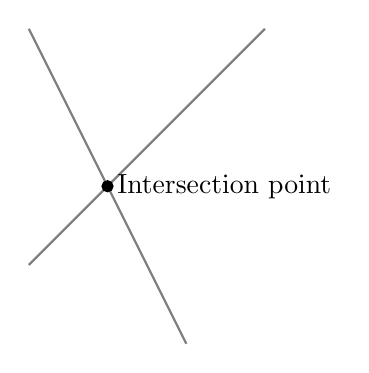
\begin{tikzpicture}
   \draw[gray, thick] (-1,2) -- (1,-2);
   \draw[gray, thick] (-1,-1) -- (2,2);
   \filldraw[black] (0,0) circle (2pt) node[anchor=west] {Intersection point};
  \end{tikzpicture}
  \begin{tikzpicture}
    \draw (-2,0) -- (2,0);
    \filldraw [gray] (0,0) circle (2pt);
    \draw (-2,-2) .. controls (0,0) .. (2,-2);
    \draw (-2,2) .. controls (-1,0) and (1,0) .. (2,2);
  \end{tikzpicture}
  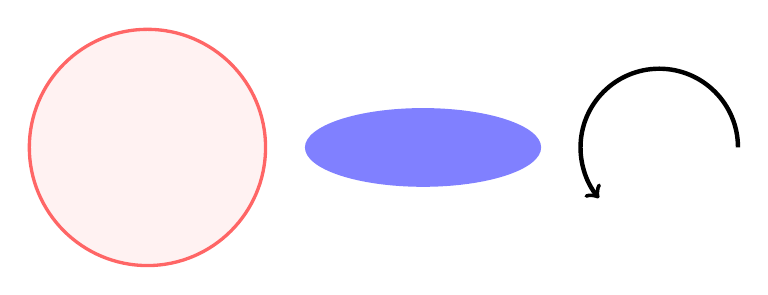
\begin{tikzpicture}
    \filldraw[color=red!60, fill=red!5, very thick](-1,0) circle (1.5);
    \fill[blue!50] (2.5,0) ellipse (1.5 and 0.5);
    \draw[ultra thick, ->] (6.5,0) arc (0:220:1);
  \end{tikzpicture}
\end{tcblisting}

\begin{tcblisting}{title=画图}
  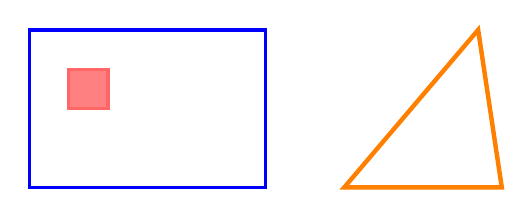
\begin{tikzpicture}
    \filldraw[color=red!60, fill=red!50, very thick](1,1) rectangle (0.5,1.5);
    \draw[blue, very thick] (0,0)rectangle (3,2);
    \draw[orange, ultra thick] (4,0) -- (6,0) -- (5.7,2) -- cycle;
  \end{tikzpicture}
\end{tcblisting}

%% 关联图
\tikz[remember picture] \node[fill=green!30] (n3) {$\sum_{n=1}^{\infty}\frac{1}{n^2}=\frac{\pi^2}{6}$};

\tikz[remember picture]
\node[
	color=red!20,
%	circle,
	draw,
%	label=angle:text,
	fill=red,
	] (nodename) {
	contents
};

%
here is some text\quad\qquad\tikz[remember picture]
\node[
color=yellow!10,
%	circle,
draw,
%	label=angle:text,
fill=blue!20,
] (n1) {
	$\sum_{n=1}^{\infty}$
};

\tikz[remember picture]
\draw[overlay,->,very thick,red,opacity=.5]
(nodename) to[bend left] (n1);

here is a circle I will type more words: \tikz[remember picture] \node[fill=red!50] (n1) {$f(x)=\sin x$};

here is a node: \tikz[remember picture] \node[fill=blue!50] (n2) {$f(x)=\sin x$};

\begin{tikzpicture}[remember picture,overlay]
	\draw[->,very thick] (n1) -- (n2);
\end{tikzpicture}

\begin{tikzpicture}[remember picture]
	\node (c) [fill=yellow!20] {Big circle};
	
	\draw[overlay,->,very thick,red,opacity=.5]
	(c) to[bend right] (n1) (n1) -| (n2) (n3) to[bend left] (n1);
\end{tikzpicture}

\begin{tcblisting}{title=270226}
  \definecolor{myred}{RGB}{183,18,52}
  \definecolor{myyellow}{RGB}{254,213,1}
  \definecolor{myblue}{RGB}{0,80,198}
  \definecolor{mygreen}{RGB}{0,155,72}
  \begin{tikzpicture}[
    line join=round,
    y={(-0.86cm,0.36cm)},x={(1cm,0.36cm)}, z={(0cm,1cm)},
    arr/.style={-latex,ultra thick,line cap=round,shorten <= 1.5pt}
  ]
  \def\Side{2}
  \coordinate (A1) at (0,0,0);
  \coordinate (A2) at (0,\Side,0);
  \coordinate (A3) at (\Side,\Side,0);
  \coordinate (A4) at (\Side,0,0);
  \coordinate (B1) at (0,0,\Side);
  \coordinate (B2) at (0,\Side,\Side);
  \coordinate (B3) at (\Side,\Side,\Side);
  \coordinate (B4) at (\Side,0,\Side);

  \fill[myyellow] (A2) -- (A3) -- (B3) -- (B2) -- cycle;
  \fill[mygreen]  (A2) -- (A3) -- (A4) -- (A1) -- cycle;
  \fill[myred](A3) -- (B3) -- (B4) -- (A4) -- cycle;
  \fill[myblue]   (A1) -- (A2) -- (B2) -- (B1) -- cycle;

  \draw (A2) -- (A1) -- (A4);
  \draw (B2) -- (B1) -- (B4) -- (B3) -- cycle;
  \draw (A1) -- (B1);
  \draw (A2) -- (B2);
  \draw (A4) -- (B4);

  \draw[thin] (A3) -- (B3);
  \draw[thin] (A3) -- (A4);

  \path[arr] 
    (A1) edge (A2)
    (B2) edge (A2)
    (B1) edge (B2)
    (B1) edge (A1)
    (B4) edge (A4)
    (B3) edge (A3)
    (B4) edge (B3)
    (A4) edge (A3);

  \node[below] at (A1) {$A$};
  \node[below] at (A2) {$B$};
  \node[below] at (A3) {$C$};
  \node[below] at (A4) {$D$};
  \node[above] at (B1) {$E$};
  \node[above] at (B2) {$F$};
  \node[above] at (B3) {$G$};
  \node[above] at (B4) {$H$};
  \end{tikzpicture}
\end{tcblisting}

\begin{tcblisting}{title=根据三点画弧}
  \begin{tikzpicture}
    \tkzDefPoint(1,2){A}
    \tkzDefPoint(3,4){B}
    \tkzDefPoint(2,4){C}
    \tkzCircumCenter(A,B,C)\tkzGetPoint{O}
    \tkzDrawArc(O,C)(A)
  \end{tikzpicture}
\end{tcblisting}


\begin{tcblisting}{title=字体}
  $\mathscr{ABCDEFGHIJKLMNOPQRSTUVWXYZ}$\\
  $\mathbb{ABCDEFGHIJKLMNOPQRSTUVWXYZ}$\\
  $\mathcal{ABCDEFGHIJKLMNOPQRSTUVWXYZ}$\\
  $\mathfrak{ABCDEFGHIJKLMNOPQRSTUVWXYZ}$
\end{tcblisting}

\section{pstricks}
{\black this is black.}
{\darkgray this is darkgray.}
{\gray this is gray.}
{\lightgray this is lightgray.}
{\white this is white.}

{\red this is red.}
{\green this is green.}
{\blue this is blue.}
{\cyan this is cyan.}
{\magenta this is magenta.}
{\yellow this is yellow.}

%{\psset{linecolor=green,linestyle=dotted}\psline(8,7)}

%\begin{tcblisting}
%	
%\end{tcblisting}
\newpage


% \chapter{math.stackexchange.com}
%%%%%%%%%%%%%%%%%%%%%%%%%%%%%%%%%%%%%%%%%%%%%%%
%%%%%%%%%%%%%%%%%%%%%%%%%%%%%%%%%%%%%%%%%%%%%%%
\bqq[breakable]{1. What Does it Really Mean to Have Different Kinds of Infinities?}{1}
What Does it Really Mean to Have Different Kinds of Infinities?

Can someone explain to me how there can be different kinds of infinities?

I was reading \href{http://en.wikipedia.org/wiki/The_Man_Who_Loved_Only_Numbers}{The man who loved only numbers}
by \href{http://en.wikipedia.org/wiki/Paul_Hoffman_(science_writer)}{Paul Hoffman}
and came across the concept of countable and uncountable infinities,
but they're only words to me.

Any help would be appreciated. 
\bs
Suppose no one ever taught you the names for ordinary numbers. Then
suppose that you and I agreed that we would trade one bushel of corn
for each of my sheep. But there's a problem, we don't know how to
count the bushels or the sheep! So what do we do?

We form a  bijection between the two
sets. That's just fancy language for saying you pair things up by
putting one bushel next to each of the sheep. When we're done we swap.
We've just proved that the number of sheep is the same as the number
of bushels without actually counting.

We can try doing the same thing with infinite sets. So suppose you
have the set of positive integers and I have the set of rational numbers
and you want to trade me one positive integer for each of my rationals.
Can you do so in a way that gets all of my rational numbers?

Perhaps surprisingly the answer is yes! You make the rational numbers
into a big square grid with the numerator and denominators as the
two coordinates. Then you start placing your  bushels
along diagonals of increasing size, \href{http://en.wikipedia.org/wiki/File:Pairing_natural.svg}{see wikipedia}.

This says that the rational numbers are  countable
that is you can find a clever way to count them off in the above fashion.

The remarkable fact is that for the real numbers there's no way at
all to count them off in this way. No matter how clever you are you
won't be able to scam me out of all of my real numbers by placing
a natural number next to each of them. The proof of that is Cantor's
clever \href{http://en.wikipedia.org/wiki/Cantor's_diagonal_argument}{diagonal argument}.
\bm
Fantastic answer! -- Allain Lalonde

I like this so far, but maybe add a bit on uncountable to distinguish
the difference. -- BBischof

That's a really good answer, thanks :D -- fbstj

Why can't lecturers at Uni explain things in this way? -- Sachin
Kainth

In the case of positives and rationals how you match them? How diagonals
become  bushels . Can u explain more on
that figure -- user5507

+1 for  fancy language -- Tyler Langan

Wow, great way to explain it. -- Abhimanyu Pallavi Sudhir

One bushel of corn for each sheep is a little too generous for me.
:P -- BlackAdder

OMG I love the bushels and the sheep. Very great way to explain it.
-- Brian Cheung

I assume with  positive numbers you mean
 positive integers . Because, after all,
$\pi$ is a positive number as well. -- celtschk
\em
\es
\bs
\textbf{How there can be different kinds of infinities?}

This is very simple to see. This is because of:

Claim: A given set $X$ and its power set $P(X)$ can never be in
bijection. 

Proof: By contradiction. Let $f$ be any function from $X$ to $P(X)$.
It suffices to prove $f$ cannot be surjective. That means that some
member of $P(X)$ i.e., some subset of $S$, is not in the image of
$f$. Consider the set:

$T=\{ x\in X: x\not\in f(x) \}.$

For every $x$ in $X$ , either $x$ is in $T$ or not. If $x$ is
in $T$, then by definition of $T$, $x$ is not in $f(x)$, so $T$
is not equal to $f(x)$. On the other hand, if $s$ is not in $T$,
then by definition of $T$, $x$ is in $f(x)$, so again $T$ is not
equal to $f(x)$. Q.E.D.

Thus take any infinite set you like. Then take its power set, its
power set, and so on. You get an infinite sequence of sets of increasing
cardinality(Here I am skipping a little; but a use of the Schroeder-Bernstein
theorem will fix things).

\href{http://en.wikipedia.org/wiki/Hilbert\%27s_paradox_of_the_Grand_Hotel}{Hilbert's Hotel}
is a classic demonstration.
\es
\bs
\href{http://en.wikipedia.org/wiki/Hilbert\%27s_paradox_of_the_Grand_Hotel}{Hilbert's Hotel} is a classic demonstration.
\bm
A really good book on the subject was written by David Wallace Foster, 
\href{http://www.amazon.co.uk/Everything-More-Compact-History-Infinity/dp/0753818825/ref=ntt_at_ep_dpt_10}{Everything and More: A Compact History of Infinity} – FordBuchanan

David Foster Wallace. (RIP :-( ) – Jason S
\em
\es
\bs
A \textbf{countably infinite} set is a set for which you can list
the elements $a_1,a_2,a_3,...$

For example, the set of all integers is countably infinite since I
can list its elements as follows: 

$0,1,-1,2,-2,3,-3,...$ 

So is the set of rational numbers, but this is more difficult to see.
Let's start with the positive rationals. Can you see the pattern in
this listing?

$\frac{1}{1},\frac{1}{2},\frac{2}{1},\frac{1}{3},\frac{2}{2},\frac{3}{1},\frac{1}{4},\frac{2}{3},\frac{3}{2},\frac{4}{1},\frac{1}{5},\frac{2}{4},...$

(Hint: Add the numerator and denominator to see a different pattern.) 

This listing has lots of repeats, e.g. $\frac{1}{1}, \frac{2}{2}$
and $\frac{1}{2}, \frac{2}{4}$. That's ok since I can condense the
listing by skipping over any repeats.

$\frac{1}{1},\frac{1}{2},\frac{2}{1},\frac{1}{3},\frac{3}{1},\frac{1}{4},\frac{2}{3},\frac{3}{2},\frac{4}{1},\frac{1}{5},...$

Let's write $q_n$ for the $n$-th element of this list. Then $0,q_1,-q_1,q_2,-q_2,q_3,-q_3,...$
is a listing of all rational numbers.

A \textbf{countable set} is a set which is either finite or countably
infinite; an \textbf{uncountable set} is a set which is not countable.

Thus, an uncountable set is an infinite set which has no listing of
all of its elements (as in the definition of countably infinite set).

An example of an uncountable set is the set of all real numbers. To
see this, you can use the \textbf{diagonal method}. Ask another question
to see how this works...
\es
\bs
You can see that there are infinitely many natural numbers $1, 2, 3, \ldots$, 
and infinitely many real numbers, such as $0, 1, \pi$, etc. 
But are these two infinities the same?

Well, suppose you have two sets of objects, e.g. people and horses, 
and you want to know if the number of objects in one set is the same as in the other. 
The simplest way is to find a way of corresponding the objects one-to-one. 
For instance, if you see a parade of people riding horses, 
you will know that there are as many people as there are horses, 
because there is such a one-to-one correspondence.

We say that a set with infinitely many things is ``countable", 
if we can find a one-to-one correspondence between the things in this set and the natural numbers.

E.g., the integers are countable: $1 \leftrightarrow 0$, $2 \leftrightarrow -1$, $3 \leftrightarrow 1$, 
$4 \leftrightarrow -2$, $5 \leftrightarrow 2$, etc, gives such a correspondence.

However, the set of real numbers is NOT countable! 
This was proven for the first time by Georg Cantor. 
Here is a proof using the so-called \href{http://en.wikipedia.org/wiki/Cantor's\_diagonal\_argument}{diagonal argument}.
\es
\bs
Infinity is an overloaded term that can mean many things.

One common non-mathematical use of infinity is to refer to 
everything in the universe. This is {\bf not} what mathematicians mean 
when they say infinity. That would be a kin to the set of all sets, 
which is a paradoxical concept that is not part of mathematical discourse.

Mathematicians will use infinity as a way to represent a process that 
continues indefinitely. This is a kin to saying ``take the limit as $n$ goes 
to infinity", which is close to saying ``continue this process indefinitely."

Infinity is also use infinity to talk about size. All sets are either infinite or finite.

The story doesn't stop there. There is something fundamentally different about 
sets like the points on a line, where there are no holes, and sets like the 
integers where there are holes. They are both infinite but one seems denser 
than the other. 

That's where whole countable uncountable thing comes in. Infinite sets 
have a size, but it is not a number in the traditional sense. Its more 
like ``relative size". Bijections are how we determine size for infinite sets, 
which are explained well on this page, so I won't repeat the explanation. 

A more in-depth, but still understandable explanation is given in 
Computability and Logic by George Boolos.
\es
\bs
The basic concept is thus:
\begin{itemize}
 \item A 'countable' infinity is one where you can give each item 
 in the set an integer and 'count' them (even though there are 
 an infinite number of them)
 \item An 'uncountable' infinity defies this. You cannot assign 
 an integer to each item in the set because you will miss items.
\end{itemize}

The key to seeing this is using the 'diagonal slash' argument as 
originally put forward by Cantor. With a countable infinity, you can 
create a list of all the items in the set and assign each one a different natural number. 
This can be done with the naturals (obviously) and the complete range of 
integers (including negative numbers) and even the rational numbers 
(so including fractions). It cannot be done with the reals due to the diagonal slash argument:

\begin{enumerate}[1.]
 \item Create your list of all real numbers and assign each one an integer
 \item Create a real number with the rule that the first digit after the 
 decimal point is different from the first digit of your first number, 
 the second digit is different from the second digit of your second number, 
 and so on for all digits
 \item Try and place this number in your list of all numbers. it can't be the 
 first number, or the second or the third and so on down the list. 
 \item Reductio Ad Absurdium, your number does not exist in your countable 
 list of all real numbers and must be added on to create a new list. 
 The same process can then be done again to show the list still isn't complete.
\end{enumerate}

This shows a difference between two obviously infinite sets and leads to the 
somewhat scary conclusion that there are (at least) 2 different forms of infinity.
\es
\eqq

% \chapter{语录}
\begin{verbatim}
在我年轻的时候, 我听从建议去读庞加莱, 希尔伯特, 克莱因以及胡尔维茨等的著作,
并从中获益. 而我自己对布拉须凯, 嘉当和霍普夫的著作更为熟悉, 其实这也是中国
的传统: 在中国我们被教导要读孔夫子, 韩愈的散文以及杜甫的诗歌, 我真诚地希望
这套全集不要成为书架上的摆设, 而是在年轻数学家的手里被翻烂掉.
\end{verbatim}
% \chapter{GTM 120. weakly differentiable functions}

\section{Riew}

\subparagraph{A Borel measure $\mu$ with the properties that each subset of $\RR^{n}$
is contained within a Borel set of equal $\mu$ measure and that $\mu\left(K\right)<\infty$
for each compact set $K\subset\RR^{n}$ is called a Radon measure.}

\section{Questions}

\subparagraph{1. recall the defination of Holder space $C^{k,\alpha}\left(\overline{\Omega}\right)$
for any open set $\Omega\subset\RR^{n}$.}

\subparagraph{2. prove that $C^{k,\alpha}\left(\overline{\Omega}\right)$ is a
Banach space.}

\subparagraph{3. define Lebesgure measurable set using outer Lebesgue measure.}

\subparagraph{4. the defination of Borel set in $\RR^{n}$.}

\subparagraph{5. if $\left|\cdot\right|$ is the outer Lebesgure measure, then
for any $A,B\subset\RR^{n}$, $d\left(A,B\right)>0$ implies $\left|A\cup B\right|=\left|A\right|+\left|B\right|$.}

\subparagraph{6. using the above conclusion, prove that for any closed set in $\RR^{n}$
is measurable, so any Borel set is measurable.}

% \begin{thebibliography}{}
 \bibitem[PH]{PH} The Man Who Loved Only Numbers, The Story of Paul Erdos and The Search for Mathematical Truth; Paul Hoffman; 1999.
 \bibitem[YN]{YN} 数域的上同调; 尤尔根$\cdot$诺伊基希, 亚历山大[德], 哈尔滨工业大学.
 \bibitem[TH]{TH} Holder不等式及其应用; 田景峰, 哈明虎, 清华大学.
 \bibitem[HKZ2013on]{HKZ} Hu, W., Kukavica, I., Ziane, M.: On the regularity for the Boussinesq equations in a bounded domain, J. Math. Phys. 54(8), 081507, 10 (2013)
 \bibitem[T1997Inf]{T} R. Temam, Infinite Dimensional Dynamical Systems in Mechanics and Physics, Applied Mathematical Sciences Vol. 68
 (Springer, 1997).
 \bibitem[MJQ]{MJ} 梅加强. 数学分析[M]. 高等教育出版社, 2011.
 \bibitem[ZYC]{ZYC} 张运筹. 三角不等式及应用[M]. 上海教育出版社.
\end{thebibliography}

\newpage
\printindex
\newpage

\end{CJK}
\end{document}
